\documentclass[11pt]{article}
\usepackage[utf8]{inputenc} % Required for inputting international characters
\usepackage[T1]{fontenc} % Output font encoding for international characters
\usepackage{caption} % for table captions
\usepackage{amsmath} % for multi-line equations and piecewises
\DeclareMathOperator{\sign}{sign}
\usepackage{graphicx}
\usepackage{relsize}
\usepackage{xspace}
\usepackage{verbatim} % for block comments
\usepackage{subcaption} % for subfigures
\usepackage{enumitem} % for a) b) c) lists
\newcommand{\Cyclus}{\textsc{Cyclus}\xspace}%
\newcommand{\Cycamore}{\textsc{Cycamore}\xspace}%
\newcommand{\deploy}{\texttt{d3ploy}\xspace}%
\newcommand{\Deploy}{\texttt{D3ploy}\xspace}%
\usepackage{tabularx}
\usepackage{color}
\usepackage{multirow}
\usepackage[acronym,toc]{glossaries}
\newacronym[longplural={metric tons of heavy metal}]{MTHM}{MTHM}{metric ton of heavy metal}
\newacronym{ABM}{ABM}{agent-based modeling}
\newacronym{ACDIS}{ACDIS}{Program in Arms Control \& Domestic and International Security}
\newacronym{AHTR}{AHTR}{Advanced High Temperature Reactor}
\newacronym{ANDRA}{ANDRA}{Agence Nationale pour la gestion des D\'echets RAdioactifs, the French National Agency for Radioactive Waste Management}
\newacronym{ANL}{ANL}{Argonne National Laboratory}
\newacronym{API}{API}{application programming interface}
\newacronym{ARCH}{ARCH}{autoregressive conditional heteroskedastic}
\newacronym{ARE}{ARE}{Aircraft Reactor Experiment}
\newacronym{ARFC}{ARFC}{Advanced Reactors and Fuel Cycles}
\newacronym{ARMA}{ARMA}{autoregressive moving average}
\newacronym{ASME}{ASME}{American Society of Mechanical Engineers}
\newacronym{ATWS}{ATWS}{Anticipated Transient Without Scram}
\newacronym{BDBE}{BDBE}{Beyond Design Basis Event}
\newacronym{BIDS}{BIDS}{Berkeley Institute for Data Science}
\newacronym{BOL}{BOL}{Beginning-of-Life}
\newacronym{BSD}{BSD}{Berkeley Software Distribution}
\newacronym{CAFCA}{CAFCA}{ Code for Advanced Fuel Cycles Assessment }
\newacronym{CASL}{CASL}{Consortium for Advanced Simulation of Light Water Reactors}
\newacronym{CDTN}{CDTN}{Centro de Desenvolvimento da Tecnologia Nuclear}
\newacronym{CEA}{CEA}{Commissariat \`a l'\'Energie Atomique et aux \'Energies Alternatives}
\newacronym{CI}{CI}{continuous integration}
\newacronym{CNEC}{CNEC}{Consortium for Nonproliferation Enabling Capabilities}
\newacronym{CNEN}{CNEN}{Comiss\~{a}o Nacional de Energia Nuclear}
\newacronym{CNERG}{CNERG}{Computational Nuclear Engineering Research Group}
\newacronym{COSI}{COSI}{Commelini-Sicard}
\newacronym{COTS}{COTS}{commercial, off-the-shelf}
\newacronym{CSNF}{CSNF}{commercial spent nuclear fuel}
\newacronym{CTAH}{CTAHs}{Coiled Tube Air Heaters}
\newacronym{CUBIT}{CUBIT}{CUBIT Geometry and Mesh Generation Toolkit}
\newacronym{CURIE}{CURIE}{Centralized Used Fuel Resource for Information Exchange}
\newacronym{DAG}{DAG}{directed acyclic graph}
\newacronym{DANESS}{DANESS}{Dynamic Analysis of Nuclear Energy System Strategies}
\newacronym{DBE}{DBE}{Design Basis Event}
\newacronym{DESAE}{DESAE}{Dynamic Analysis of Nuclear Energy Systems Strategies}
\newacronym{DHS}{DHS}{Department of Homeland Security}
\newacronym{DOE}{DOE}{Department of Energy}
\newacronym{DRACS}{DRACS}{Direct Reactor Auxiliary Cooling System}
\newacronym{DRE}{DRE}{dynamic resource exchange}
\newacronym{DSNF}{DSNF}{DOE spent nuclear fuel}
\newacronym{DYMOND}{DYMOND}{Dynamic Model of Nuclear Development }
\newacronym{EBS}{EBS}{Engineered Barrier System}
\newacronym{EDZ}{EDZ}{Excavation Disturbed Zone}
\newacronym{EIA}{EIA}{U.S. Energy Information Administration}
\newacronym{EPA}{EPA}{Environmental Protection Agency}
\newacronym{EP}{EP}{Engineering Physics}
\newacronym{FCO}{FCO}{Fuel Cycle Options}
\newacronym{FCT}{FCT}{Fuel Cycle Technology}
\newacronym{FCWMD}{FCWMD}{Fuel Cycle and Waste Management Division}
\newacronym{FEHM}{FEHM}{Finite Element Heat and Mass Transfer}
\newacronym{FEPs}{FEPs}{Features, Events, and Processes}
\newacronym{FHR}{FHR}{Fluoride-Salt-Cooled High-Temperature Reactor}
\newacronym{FLiBe}{FLiBe}{Fluoride-Lithium-Beryllium}
\newacronym{GCAM}{GCAM}{Global Change Assessment Model}
\newacronym{GDSE}{GDSE}{Generic Disposal System Environment}
\newacronym{GDSM}{GDSM}{Generic Disposal System Model}
\newacronym{GENIUSv1}{GENIUSv1}{Global Evaluation of Nuclear Infrastructure Utilization Scenarios, Version 1}
\newacronym{GENIUSv2}{GENIUSv2}{Global Evaluation of Nuclear Infrastructure Utilization Scenarios, Version 2}
\newacronym{GENIUS}{GENIUS}{Global Evaluation of Nuclear Infrastructure Utilization Scenarios}
\newacronym{GPAM}{GPAM}{Generic Performance Assessment Model}
\newacronym{GRSAC}{GRSAC}{Graphite Reactor Severe Accident Code}
\newacronym{GUI}{GUI}{graphical user interface}
\newacronym{HLW}{HLW}{high level waste}
\newacronym{HPC}{HPC}{high-performance computing}
\newacronym{HTC}{HTC}{high-throughput computing}
\newacronym{HTGR}{HTGR}{High Temperature Gas-Cooled Reactor}
\newacronym{IAEA}{IAEA}{International Atomic Energy Agency}
\newacronym{IEMA}{IEMA}{Illinois Emergency Mangament Agency}
\newacronym{INL}{INL}{Idaho National Laboratory}
\newacronym{IPRR1}{IRP-R1}{Instituto de Pesquisas Radioativas Reator 1}
\newacronym{IRP}{IRP}{Integrated Research Project}
\newacronym{ISFSI}{ISFSI}{Independent Spent Fuel Storage Installation}
\newacronym{ISRG}{ISRG}{Independent Student Research Group}
\newacronym{JFNK}{JFNK}{Jacobian-Free Newton Krylov}
\newacronym{LANL}{LANL}{Los Alamos National Laboratory}
\newacronym{LBNL}{LBNL}{Lawrence Berkeley National Laboratory}
\newacronym{LCOE}{LCOE}{levelized cost of electricity}
\newacronym{LDRD}{LDRD}{laboratory directed research and development}
\newacronym{LFR}{LFR}{Lead-Cooled Fast Reactor}
\newacronym{LGPL}{LGPL}{Lesser GNU Public License}
\newacronym{LLNL}{LLNL}{Lawrence Livermore National Laboratory}
\newacronym{LMFBR}{LMFBR}{Liquid-Metal-cooled Fast Breeder Reactor}
\newacronym{LOFC}{LOFC}{Loss of Forced Cooling}
\newacronym{LOHS}{LOHS}{Loss of Heat Sink}
\newacronym{LOLA}{LOLA}{Loss of Large Area}
\newacronym{LP}{LP}{linear program}
\newacronym{LWR}{LWR}{Light Water Reactor}
\newacronym{MARKAL}{MARKAL}{MARKet and ALlocation}
\newacronym{MA}{MA}{minor actinide}
\newacronym{MCNP}{MCNP}{Monte Carlo N-Particle code}
\newacronym{MILP}{MILP}{mixed-integer linear program}
\newacronym{MIT}{MIT}{the Massachusetts Institute of Technology}
\newacronym{MOAB}{MOAB}{Mesh-Oriented datABase}
\newacronym{MOOSE}{MOOSE}{Multiphysics Object-Oriented Simulation Environment}
\newacronym{MOX}{MOX}{mixed oxide}
\newacronym{MSBR}{MSBR}{Molten Salt Breeder Reactor}
\newacronym{MSRE}{MSRE}{Molten Salt Reactor Experiment}
\newacronym{MSR}{MSR}{Molten Salt Reactor}
\newacronym{NAGRA}{NAGRA}{National Cooperative for the Disposal of Radioactive Waste}
\newacronym{NCSA}{NCSA}{National Center for Supercomputing Applications}
\newacronym{NEAMS}{NEAMS}{Nuclear Engineering Advanced Modeling and Simulation}
\newacronym{NEUP}{NEUP}{Nuclear Energy University Programs}
\newacronym{NFCSim}{NFCSim}{Nuclear Fuel Cycle Simulator}
\newacronym{NFC}{NFC}{Nuclear Fuel Cycle}
\newacronym{NGNP}{NGNP}{Next Generation Nuclear Plant}
\newacronym{NMWPC}{NMWPC}{Nuclear MW Per Capita}
\newacronym{NNSA}{NNSA}{National Nuclear Security Administration}
\newacronym{NPRE}{NPRE}{Department of Nuclear, Plasma, and Radiological Engineering}
\newacronym{NQA1}{NQA-1}{Nuclear Quality Assurance - 1}
\newacronym{NRC}{NRC}{Nuclear Regulatory Commission}
\newacronym{NSF}{NSF}{National Science Foundation}
\newacronym{NSSC}{NSSC}{Nuclear Science and Security Consortium}
\newacronym{NUWASTE}{NUWASTE}{Nuclear Waste Assessment System for Technical Evaluation}
\newacronym{NWF}{NWF}{Nuclear Waste Fund}
\newacronym{NWTRB}{NWTRB}{Nuclear Waste Technical Review Board}
\newacronym{OCRWM}{OCRWM}{Office of Civilian Radioactive Waste Management}
\newacronym{ORION}{ORION}{ORION}
\newacronym{ORNL}{ORNL}{Oak Ridge National Laboratory}
\newacronym{PARCS}{PARCS}{Purdue Advanced Reactor Core Simulator}
\newacronym{PBAHTR}{PB-AHTR}{Pebble Bed Advanced High Temperature Reactor}
\newacronym{PBFHR}{PB-FHR}{Pebble-Bed Fluoride-Salt-Cooled High-Temperature Reactor}
\newacronym{PEI}{PEI}{Peak Environmental Impact}
\newacronym{PH}{PRONGHORN}{PRONGHORN}
\newacronym{PI}{PI}{Principal Investigator}
\newacronym{PNNL}{PNNL}{Pacific Northwest National Laboratory}
\newacronym{PRIS}{PRIS}{Power Reactor Information System}
\newacronym{PRKE}{PRKE}{Point Reactor Kinetics Equations}
\newacronym{PSPG}{PSPG}{Pressure-Stabilizing/Petrov-Galerkin}
\newacronym{PWAR}{PWAR}{Pratt and Whitney Aircraft Reactor}
\newacronym{PWR}{PWR}{Pressurized Water Reactor}
\newacronym{PyNE}{PyNE}{Python toolkit for Nuclear Engineering}
\newacronym{PyRK}{PyRK}{Python for Reactor Kinetics}
\newacronym{QA}{QA}{quality assurance}
\newacronym{RDD}{RD\&D}{Research Development and Demonstration}
\newacronym{RD}{R\&D}{Research and Development}
\newacronym{RELAP}{RELAP}{Reactor Excursion and Leak Analysis Program}
\newacronym{RIA}{RIA}{Reactivity Insertion Accident}
\newacronym{RIF}{RIF}{Region-Institution-Facility}
\newacronym{SAM}{SAM}{Simulation and Modeling}
\newacronym{SCF}{SCF}{Software Carpentry Foundation}
\newacronym{SFR}{SFR}{Sodium-Cooled Fast Reactor}
\newacronym{SINDAG}{SINDA{\textbackslash}G}{Systems Improved Numerical Differencing Analyzer $\backslash$ Gaski}
\newacronym{SKB}{SKB}{Svensk K\"{a}rnbr\"{a}nslehantering AB}
\newacronym{SNF}{SNF}{spent nuclear fuel}
\newacronym{SNL}{SNL}{Sandia National Laboratory}
\newacronym{SNM}{SNM}{Special Nuclear Material}
\newacronym{STC}{STC}{specific temperature change}
\newacronym{SUPG}{SUPG}{Streamline-Upwind/Petrov-Galerkin}
\newacronym{SWF}{SWF}{Separations and Waste Forms}
\newacronym{SWU}{SWU}{Separative Work Unit}
\newacronym{SandO}{S\&O}{Signatures and Observables}
\newacronym{THW}{THW}{The Hacker Within}
\newacronym{TRIGA}{TRIGA}{Training Research Isotope General Atomic}
\newacronym{TRISO}{TRISO}{Tristructural Isotropic}
\newacronym{TSM}{TSM}{Total System Model}
\newacronym{TSPA}{TSPA}{Total System Performance Assessment for the Yucca Mountain License Application}
\newacronym{UDB}{UDB}{Unified Database}
\newacronym{UFD}{UFD}{Used Fuel Disposition}
\newacronym{UML}{UML}{Unified Modeling Language}
\newacronym{UNFSTANDARDS}{UNFST\&DARDS}{Used Nuclear Fuel Storage, Transportation \& Disposal Analysis Resource and Data System}
\newacronym{UOX}{UOX}{uranium oxide}
\newacronym{UQ}{UQ}{uncertainty quantification}
\newacronym{US}{US}{United States}
\newacronym{UW}{UW}{University of Wisconsin}
\newacronym{VISION}{VISION}{the Verifiable Fuel Cycle Simulation Model}
\newacronym{VV}{V\&V}{verification and validation}
\newacronym{WIPP}{WIPP}{Waste Isolation Pilot Plant}
\newacronym{YMG}{YMG}{Young Members Group}
\newacronym{YMR}{YMR}{Yucca Mountain Repository Site}
\newacronym{NEI}{NEI}{Nuclear Energy Institute}
%\newacronym{<++>}{<++>}{<++>}
%\newacronym{<++>}{<++>}{<++>}

\definecolor{bg}{rgb}{0.95,0.95,0.95}
\newcolumntype{b}{X}
\newcolumntype{f}{>{\hsize=.15\hsize}X}
\newcolumntype{s}{>{\hsize=.5\hsize}X}
\newcolumntype{m}{>{\hsize=.75\hsize}X}
\newcolumntype{r}{>{\hsize=1.1\hsize}X}
\usepackage{titling}
\usepackage[hang,flushmargin]{footmisc}
\renewcommand*\footnoterule{}
\usepackage{tikz}
\definecolor{illiniblue}{HTML}{437db6}
\definecolor{illiniorange}{HTML}{E38749}
\usetikzlibrary{shapes.geometric, arrows}
\tikzstyle{oblock} = [rectangle, draw, fill=illiniorange, 
text width=12em, text centered, rounded corners, minimum height=4em]
\tikzstyle{bblock} = [rectangle, draw, fill=illiniblue, 
text width=12em, text centered, rounded corners, minimum height=4em]
\tikzstyle{arrow} = [thick,->,>=stealth]

\usetikzlibrary{shapes.geometric,arrows}
\tikzstyle{process} = [rectangle, rounded corners, 
minimum width=1cm, minimum height=1cm,text centered, draw=black, 
fill=blue!30]
\tikzstyle{arrow} = [thick,->,>=stealth]

\graphicspath{}
\usepackage{mathpazo} % Palatino font
\usepackage{graphicx} % For the logo
\usepackage{float} 

\usepackage[hidelinks]{hyperref}
\urlstyle{tt}

\newcolumntype{L}{>{\raggedright\arraybackslash}X}
\newcolumntype{R}{>{\raggedleft\arraybackslash}X}

\begin{document}
\title{DDCA Project Final Report}
\maketitle
\tableofcontents

\pagebreak

\section{Objective}
The objective of this report is to showcase results from the  
Demand-Driven Cycamore Archetypes project (NEUP-FY16-10512). 

\section{Eg01-Eg23}

Figure \ref{fig:23flow} shows the flow of Eg01-Eg23.

\begin{figure}[H]
	\centering
	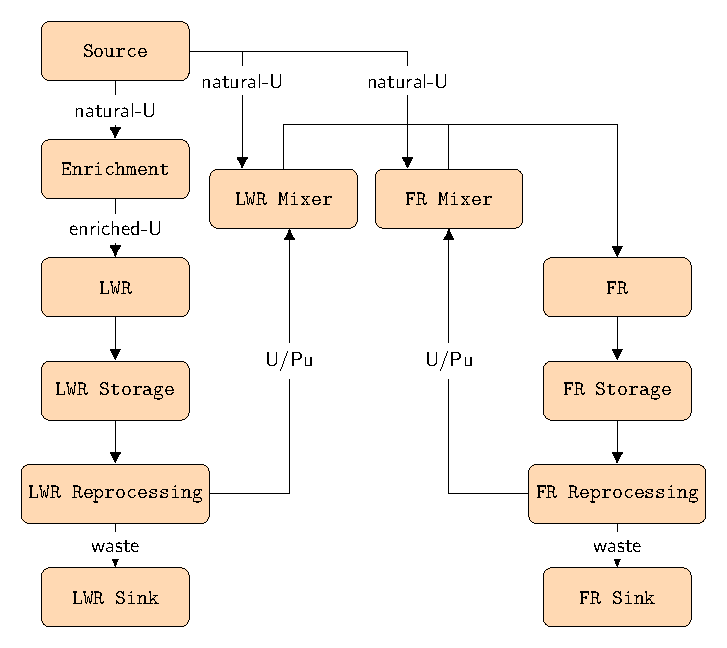
\includegraphics[width=\textwidth]{23-figures/23flow.pdf} 
	\hfill
	\caption{EG01-EG23.}
	\label{fig:23flow}
\end{figure}

\subsection{Power}

This section presents plots of power for all the prediction methods. The power demand is 60000 MW throughout the whole simulation. The input files use the installed capacity feature. Buffer is set to zero, back steps is set to two, and steps takes the default value of one.
Figures \ref{fig:23-NO}, \ref{fig:23-DO}, and \ref{fig:23-SO} display the power supply and demand.
Table \ref{tab:23-power} records the number of steps whit under supply, the cumulative under supply, and the cumulative oversupply.

\begin{figure}[H]
	\centering
	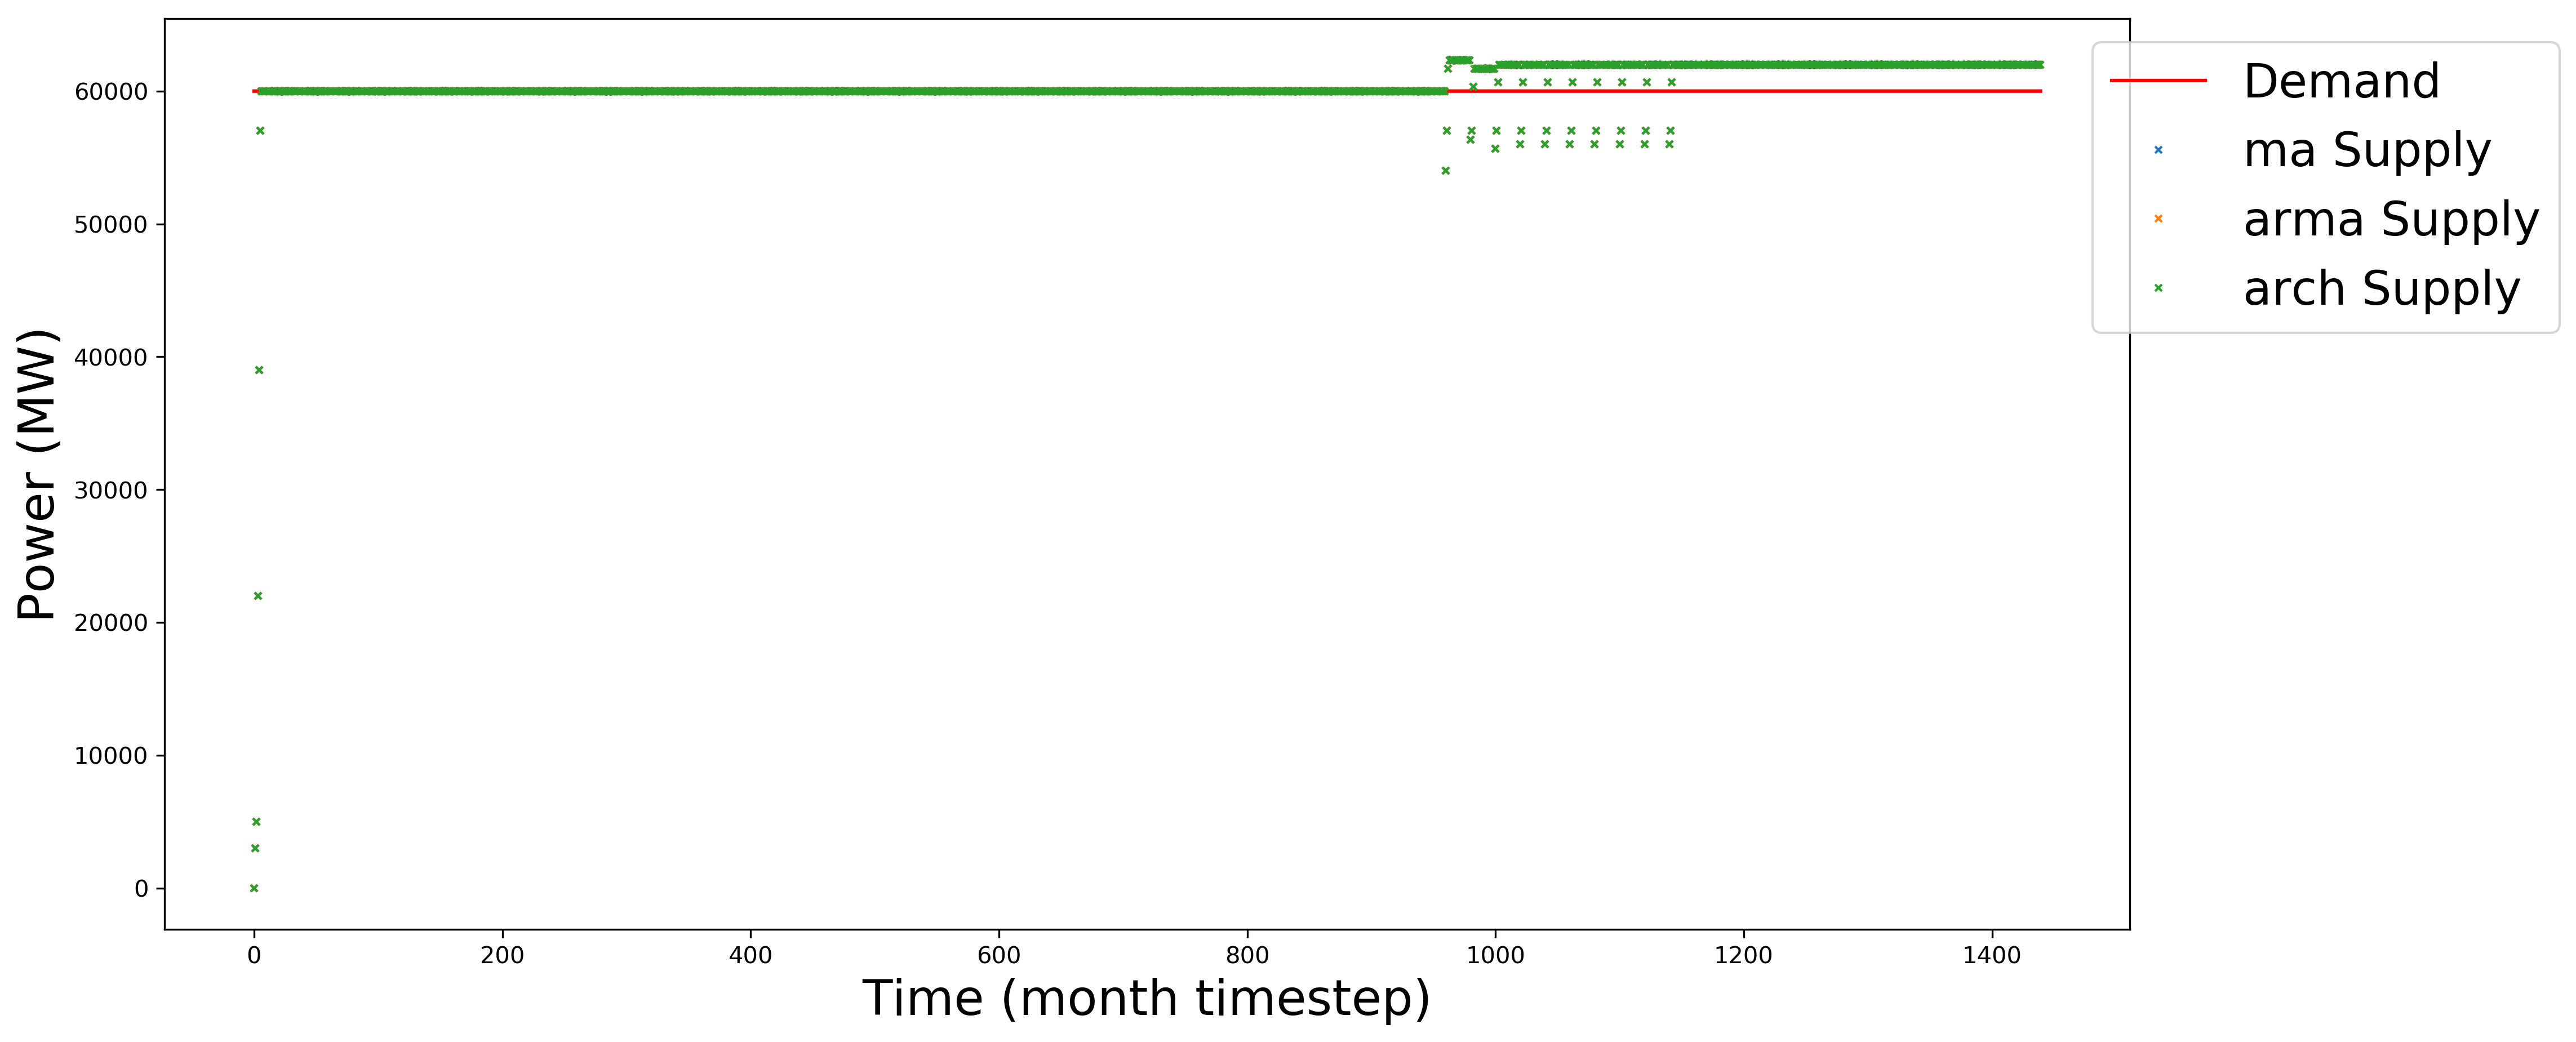
\includegraphics[width=\textwidth]{23-figures/23-power-buffer01.png} 
	\hfill
	\caption{NO algorithms.}
	\label{fig:23-NO}
\end{figure}

\begin{figure}[H]
	\centering
	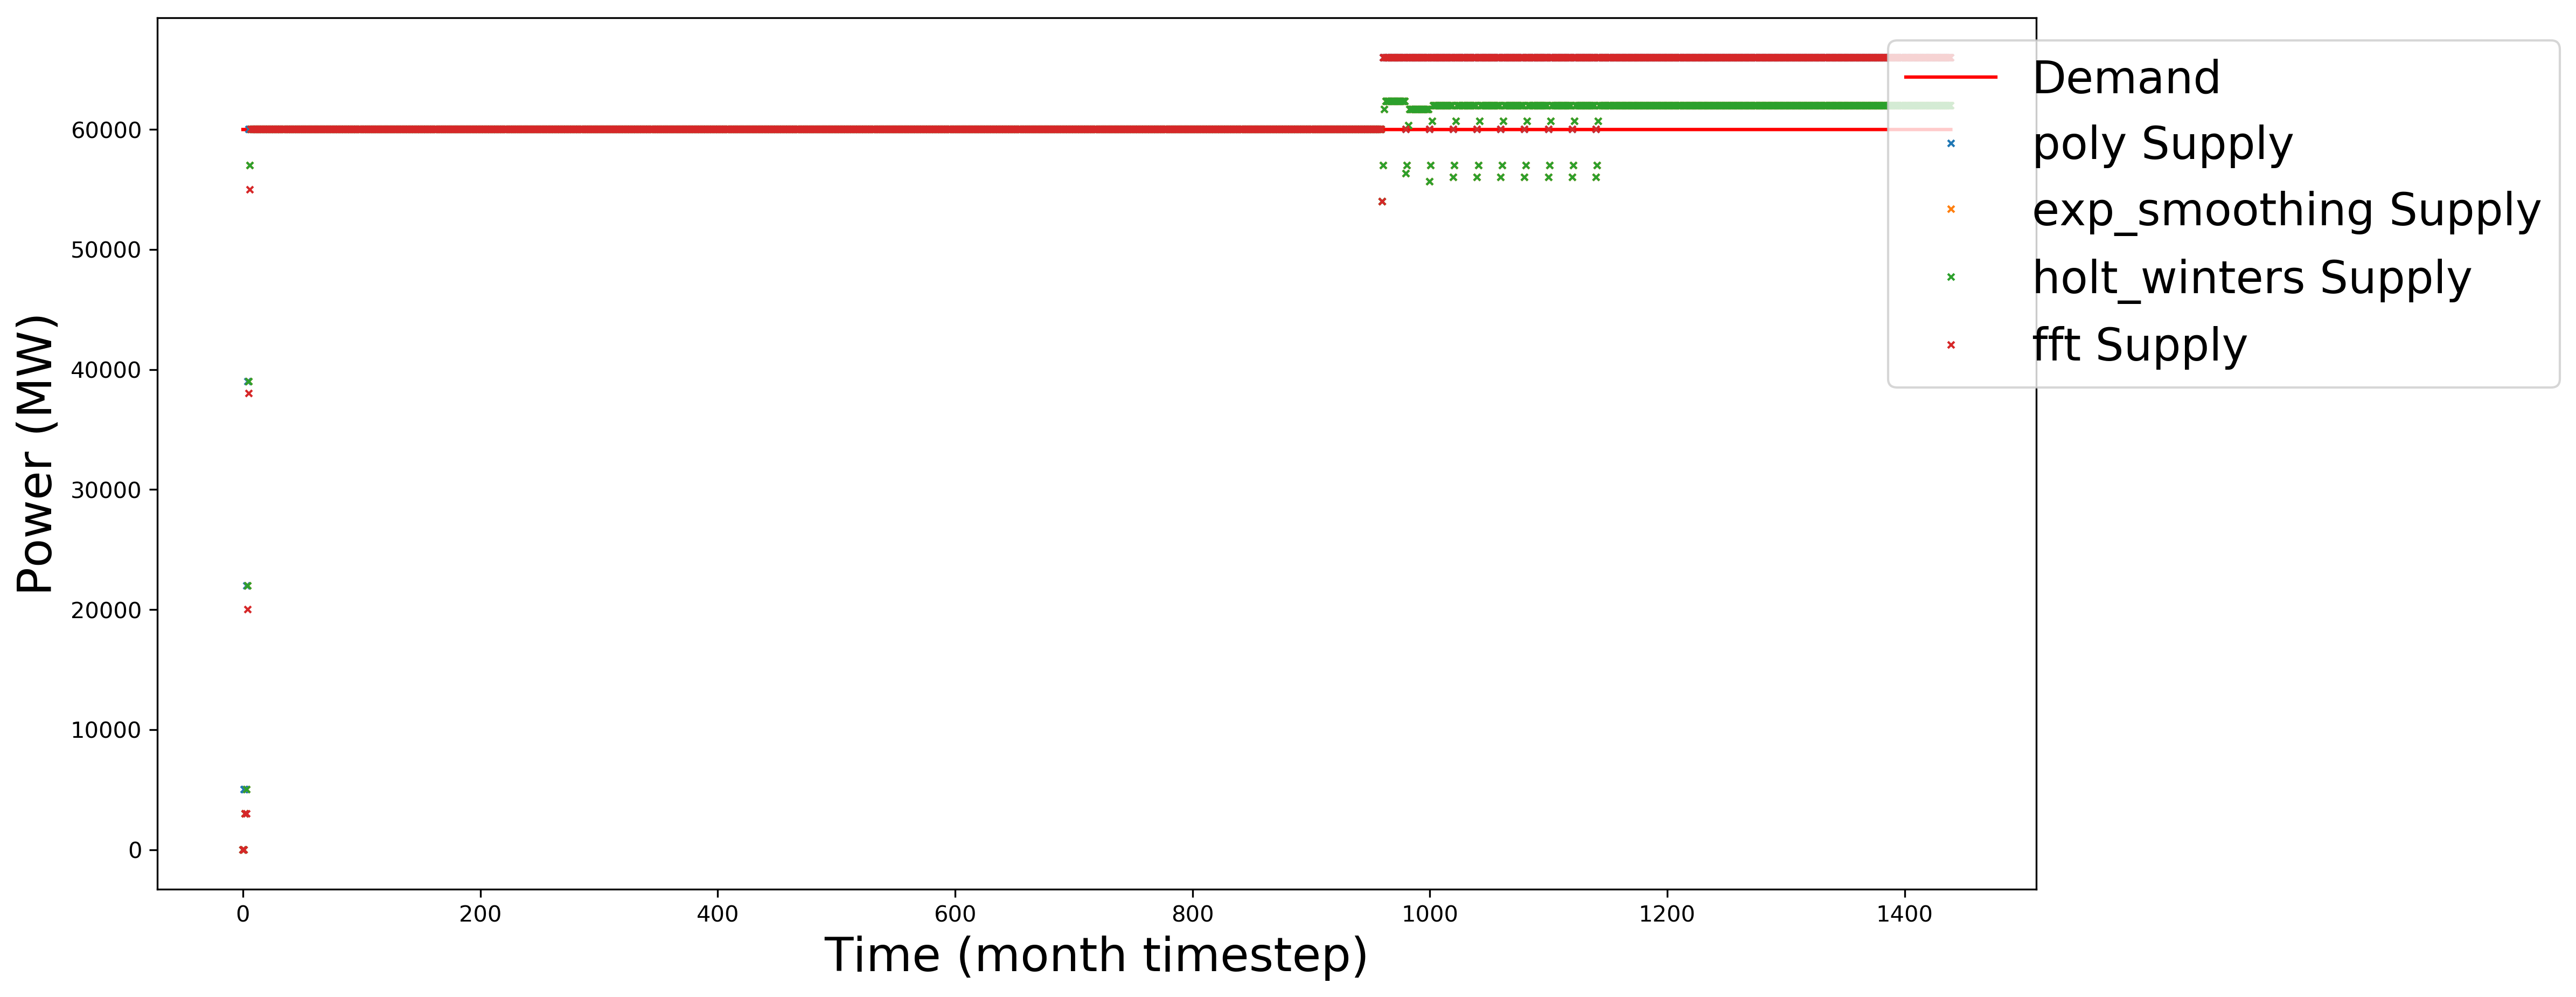
\includegraphics[width=\textwidth]{23-figures/23-power-buffer02.png} 
	\hfill
	\caption{DO algorithms.}
	\label{fig:23-DO}
\end{figure}

\begin{figure}[H]
	\centering
	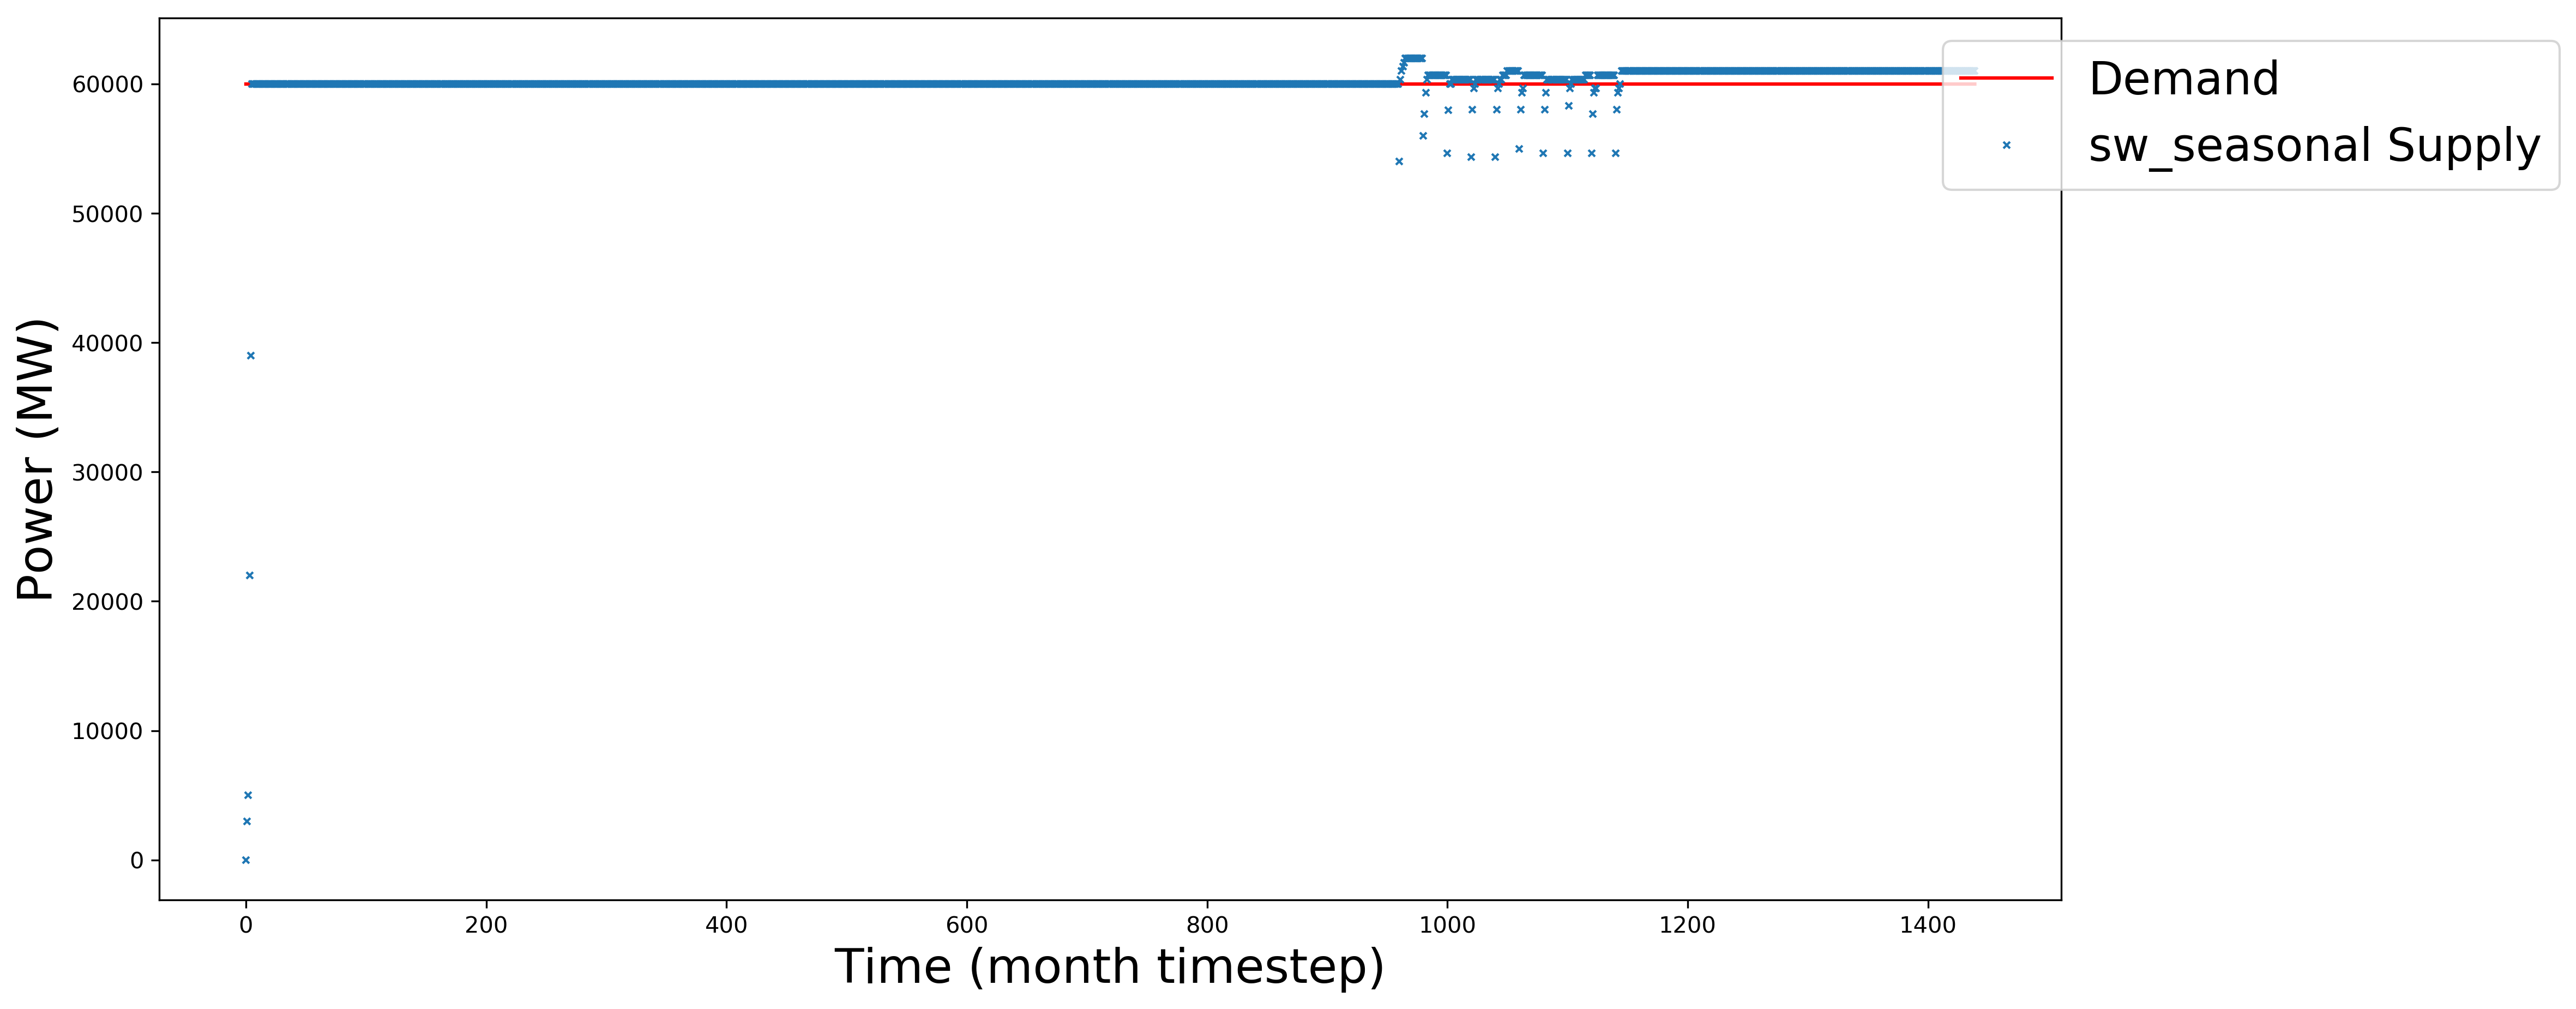
\includegraphics[width=\textwidth]{23-figures/23-power-buffer03.png} 
	\hfill
	\caption{SO algorithms.}
	\label{fig:23-SO}
\end{figure}

\begin{table}[H]
	\centering
	\caption{Undersupply and oversupply of Power for the different algorithms used to calculate EG01-EG23.}
	\label{tab:23-power}
	\begin{tabularx}{\textwidth}{lRRR}
		\hline
		Algorithm & Undersupplied & Cumulative  & Cumulative \\
		& Timesteps     & Undersupply [GW.mo]  & Oversupply [GW.mo] \\ \hline
		MA        & 26 	& 306.0 &  907.8   \\ 
		ARMA      & 26 	& 306.0 &  907.8   \\ 
		ARCH      & 26 	& 306.0 &  907.8   \\ 
		POLY      &  6 	& 235.0 &  2820.5  \\ 
		EXP\_SMOOTHING 	& 27 & 366.0 & 907.8 \\ 
		HOLT-WINTERS  	& 27 & 366.0 & 907.8 \\ 
		FFT       & 8	& 307.0	& 2820.5 \\ 
		SW\_SEASONAL    & 36 & 308.0 & 398.1	\\ \hline
	\end{tabularx}
\end{table}

\subsection{Buffer}

This section presents a sensitivity analysis for different values of the buffer. Figure \ref{fig:23-buff} shows a comparison of the cumulative under supply for different buffer sizes.

Figures \ref{fig:23-buf-ma} to \ref{fig:23-buf-fft} display a comparison for some of the methods of the power supply for different buffer sizes.

The input files use the installed capacity feature. Buffer takes the values 0, 2000, 4000, 6000, and 8000. Back steps is set to two, and steps takes the default value of one.

\begin{figure}[H]
	\centering
	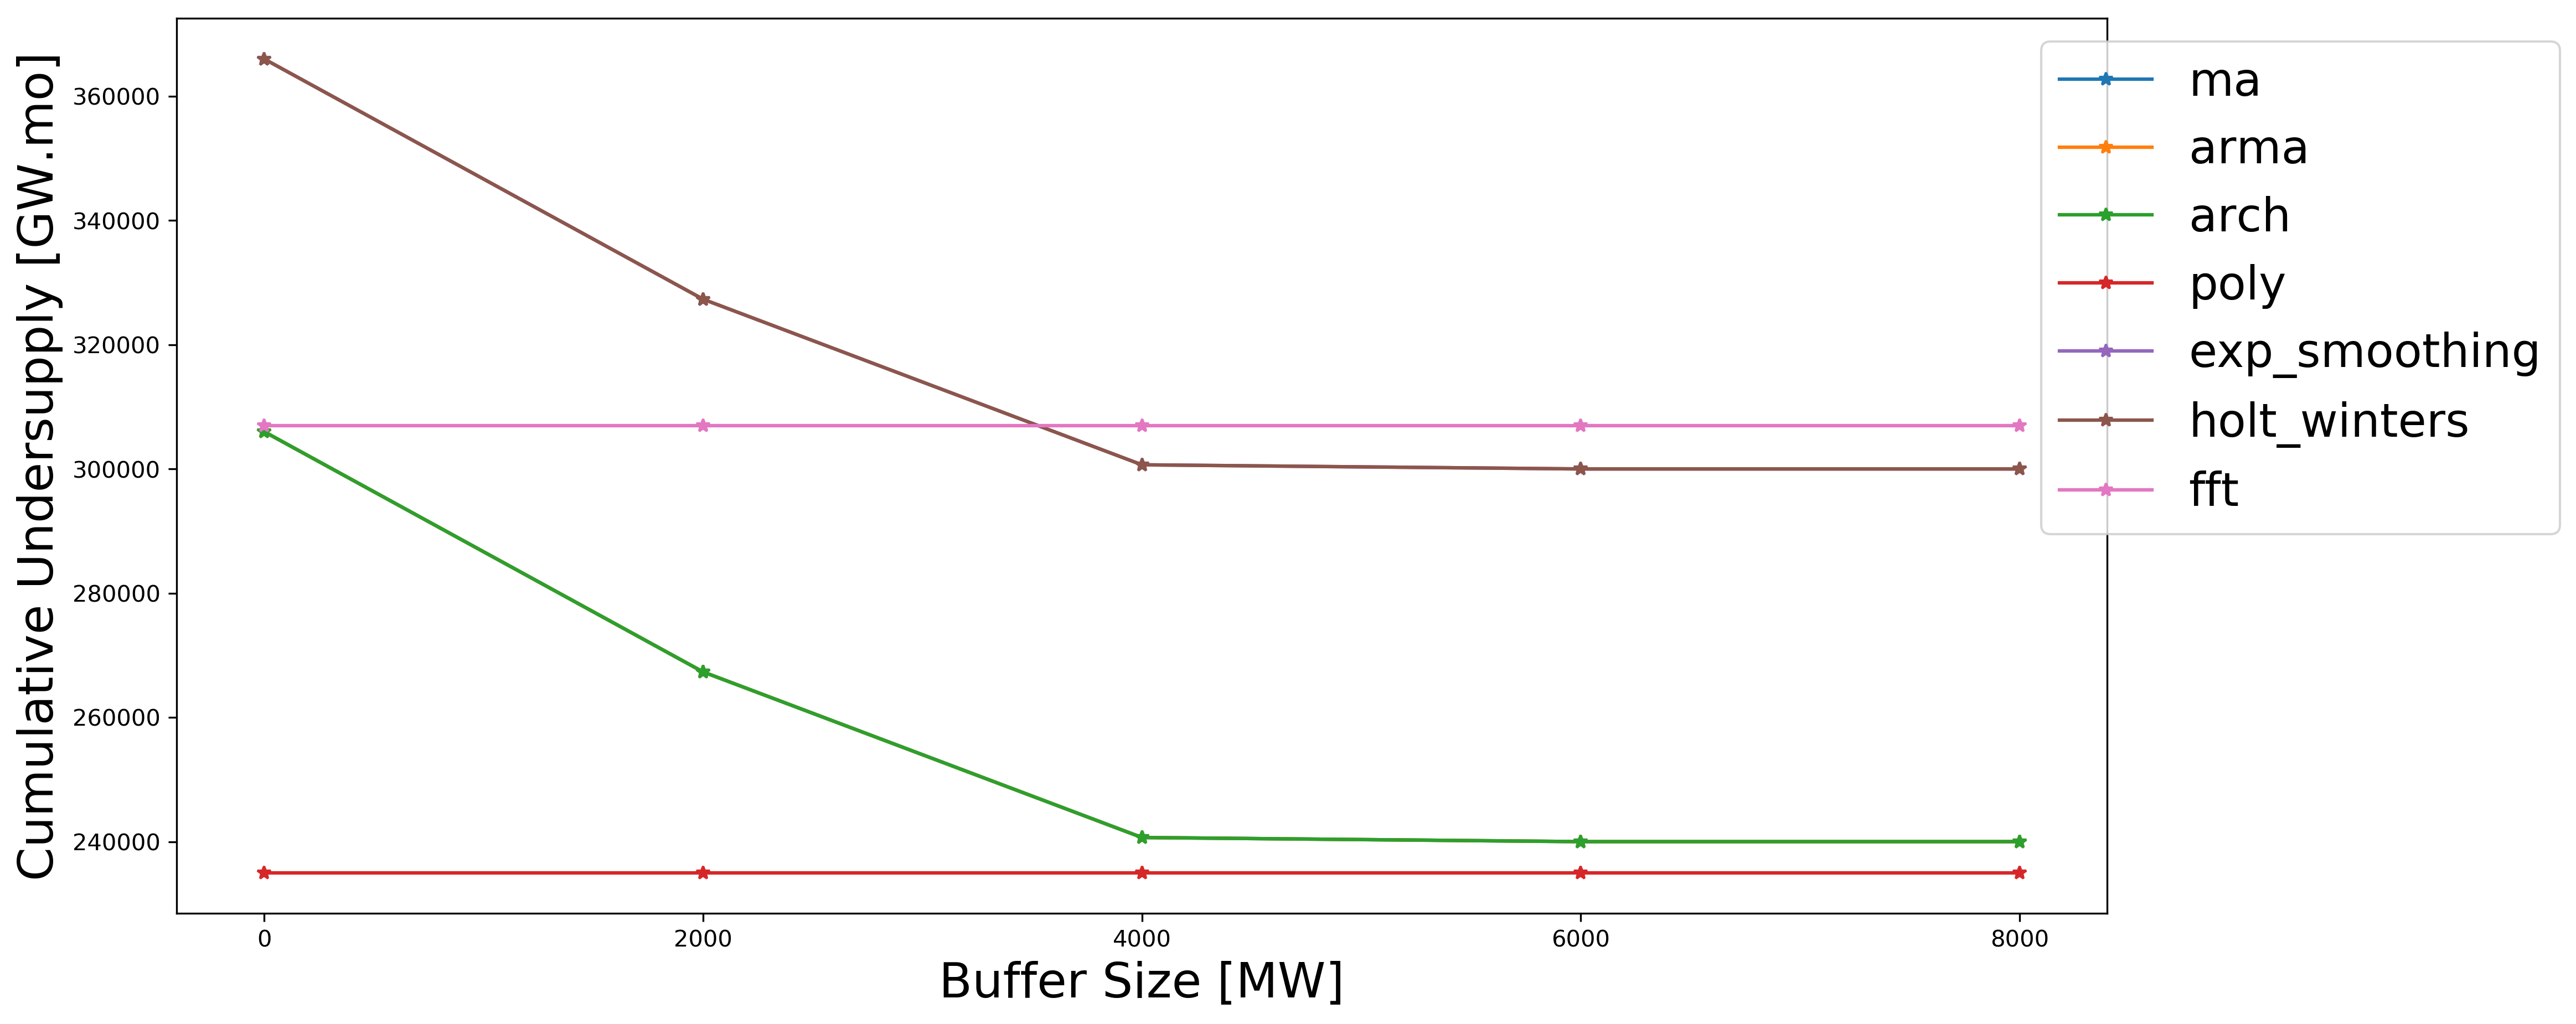
\includegraphics[width=\textwidth]{23-figures/23-sens-buffer.png} 
	\hfill
	\caption{Sensitivity analysis for different buffer sizes for some prediction algorithms.}
	\label{fig:23-buff}
\end{figure}

\begin{figure}[H]
	\centering
	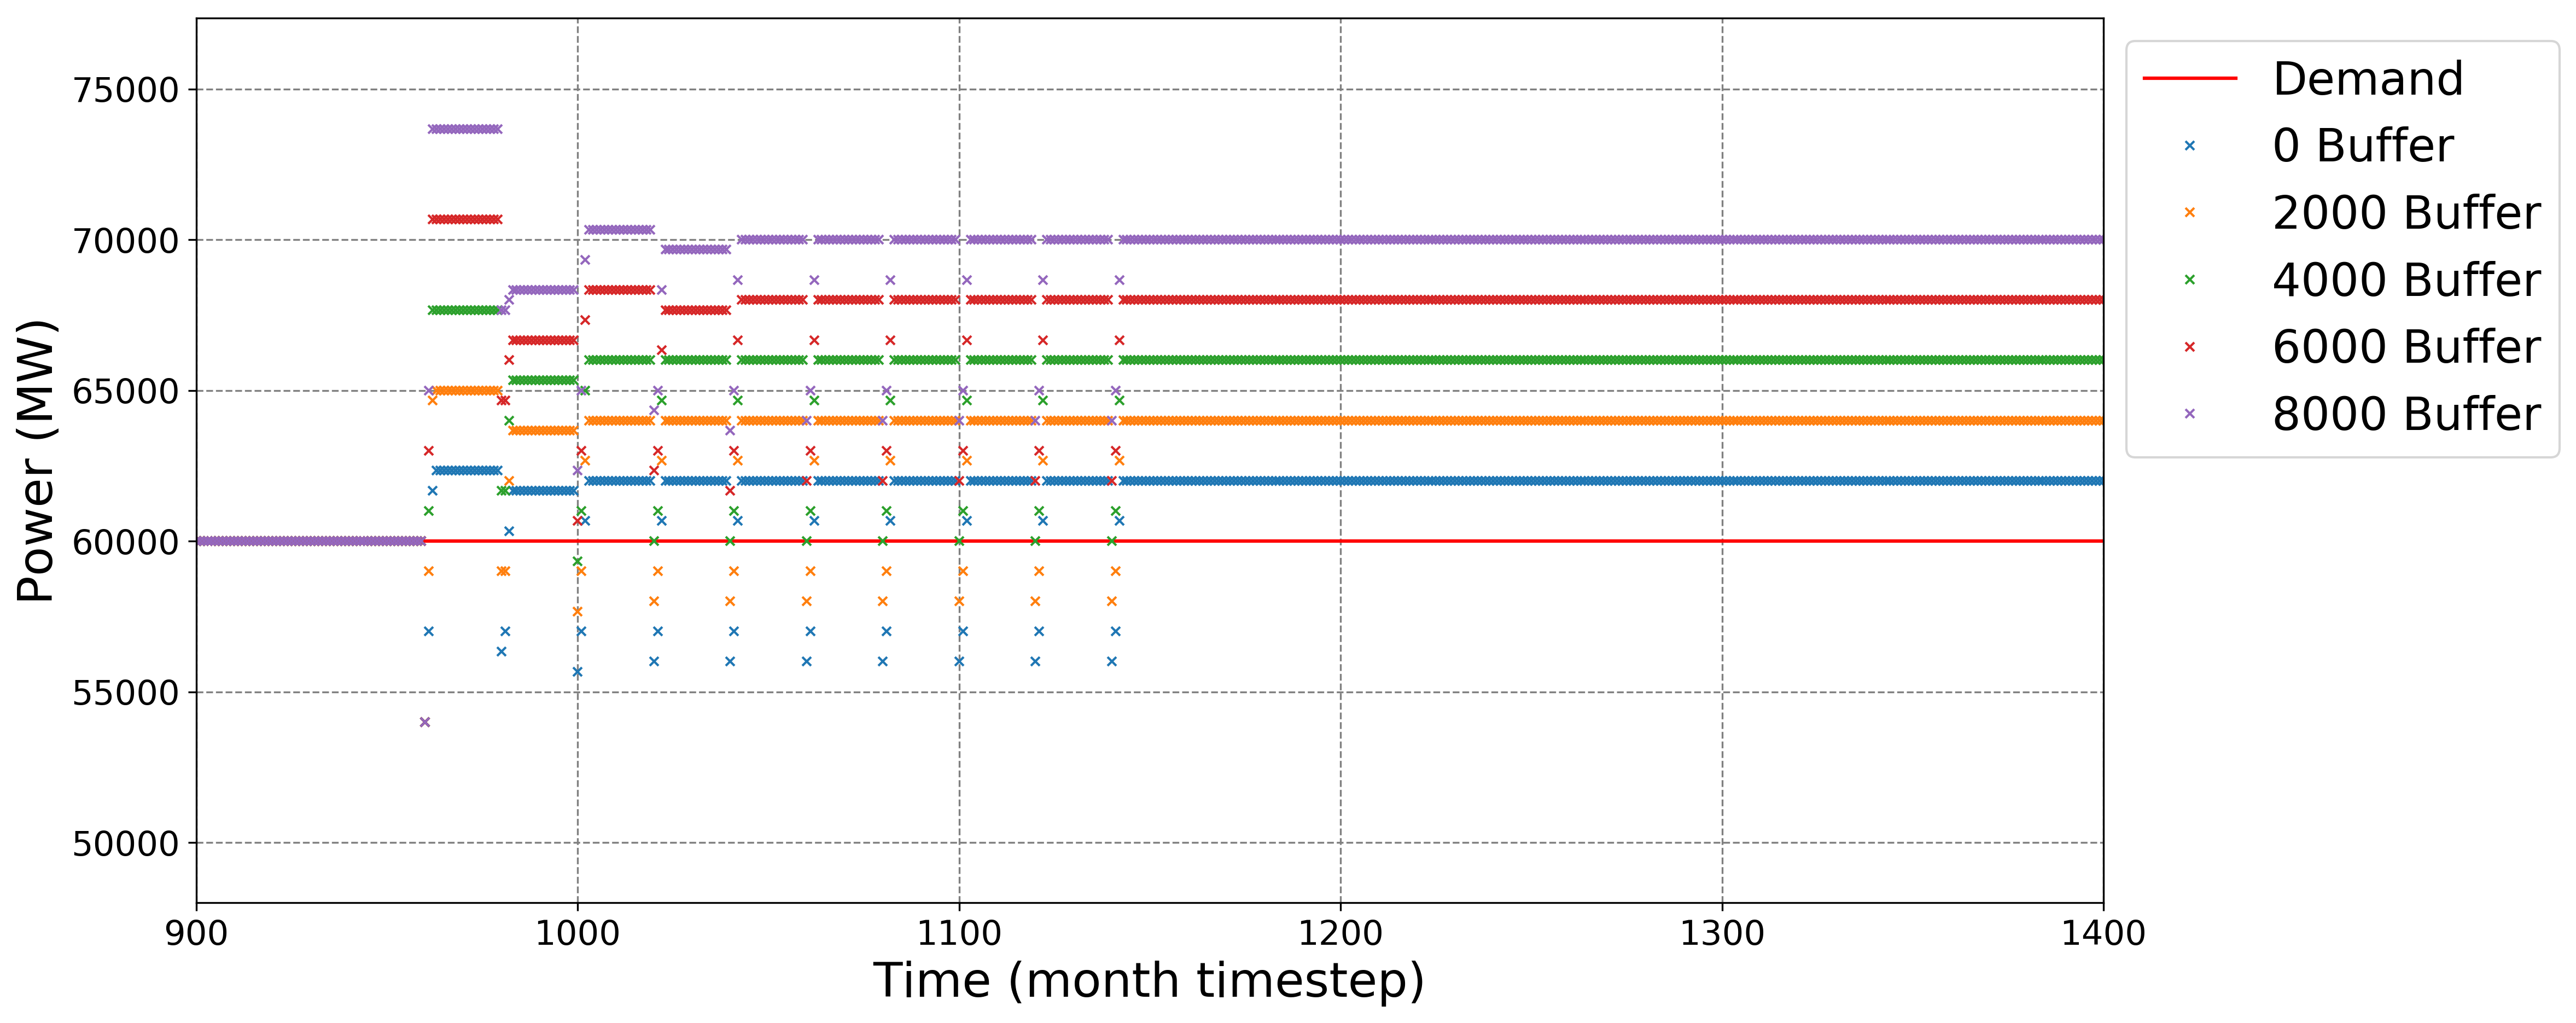
\includegraphics[width=\textwidth]{23-figures/23-power-buffer-ma.png} 
	\hfill
	\caption{Power supply for different buffer sizes using ma.}
	\label{fig:23-buf-ma}
\end{figure}

\begin{figure}[H]
	\centering
	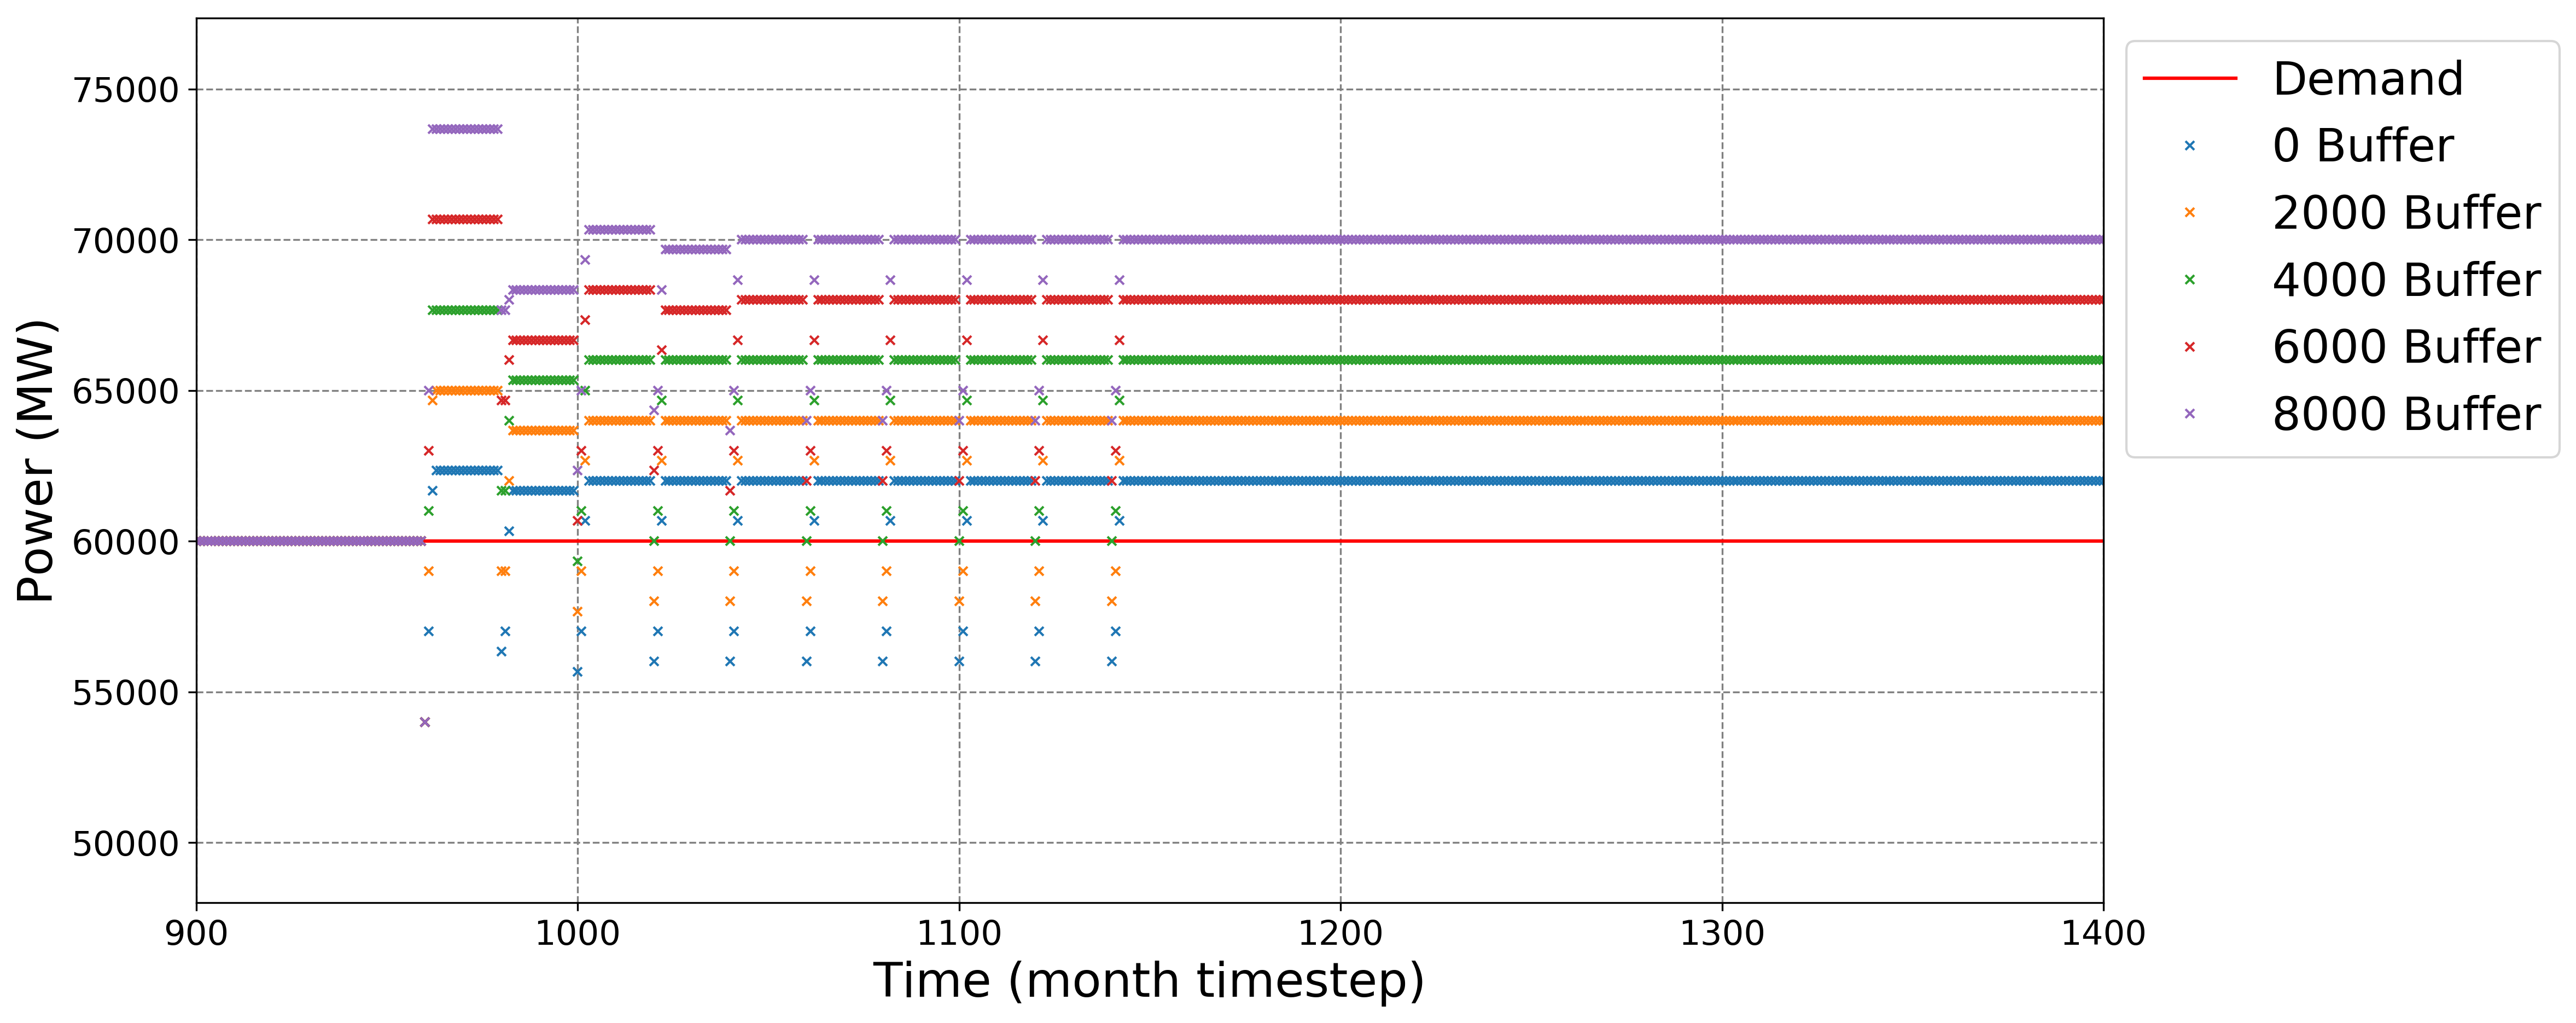
\includegraphics[width=\textwidth]{23-figures/23-power-buffer-arma.png} 
	\hfill
    \caption{Power supply for different buffer sizes using arma.}
	\label{fig:23-buf-arma}
\end{figure}

\begin{figure}[H]
	\centering
	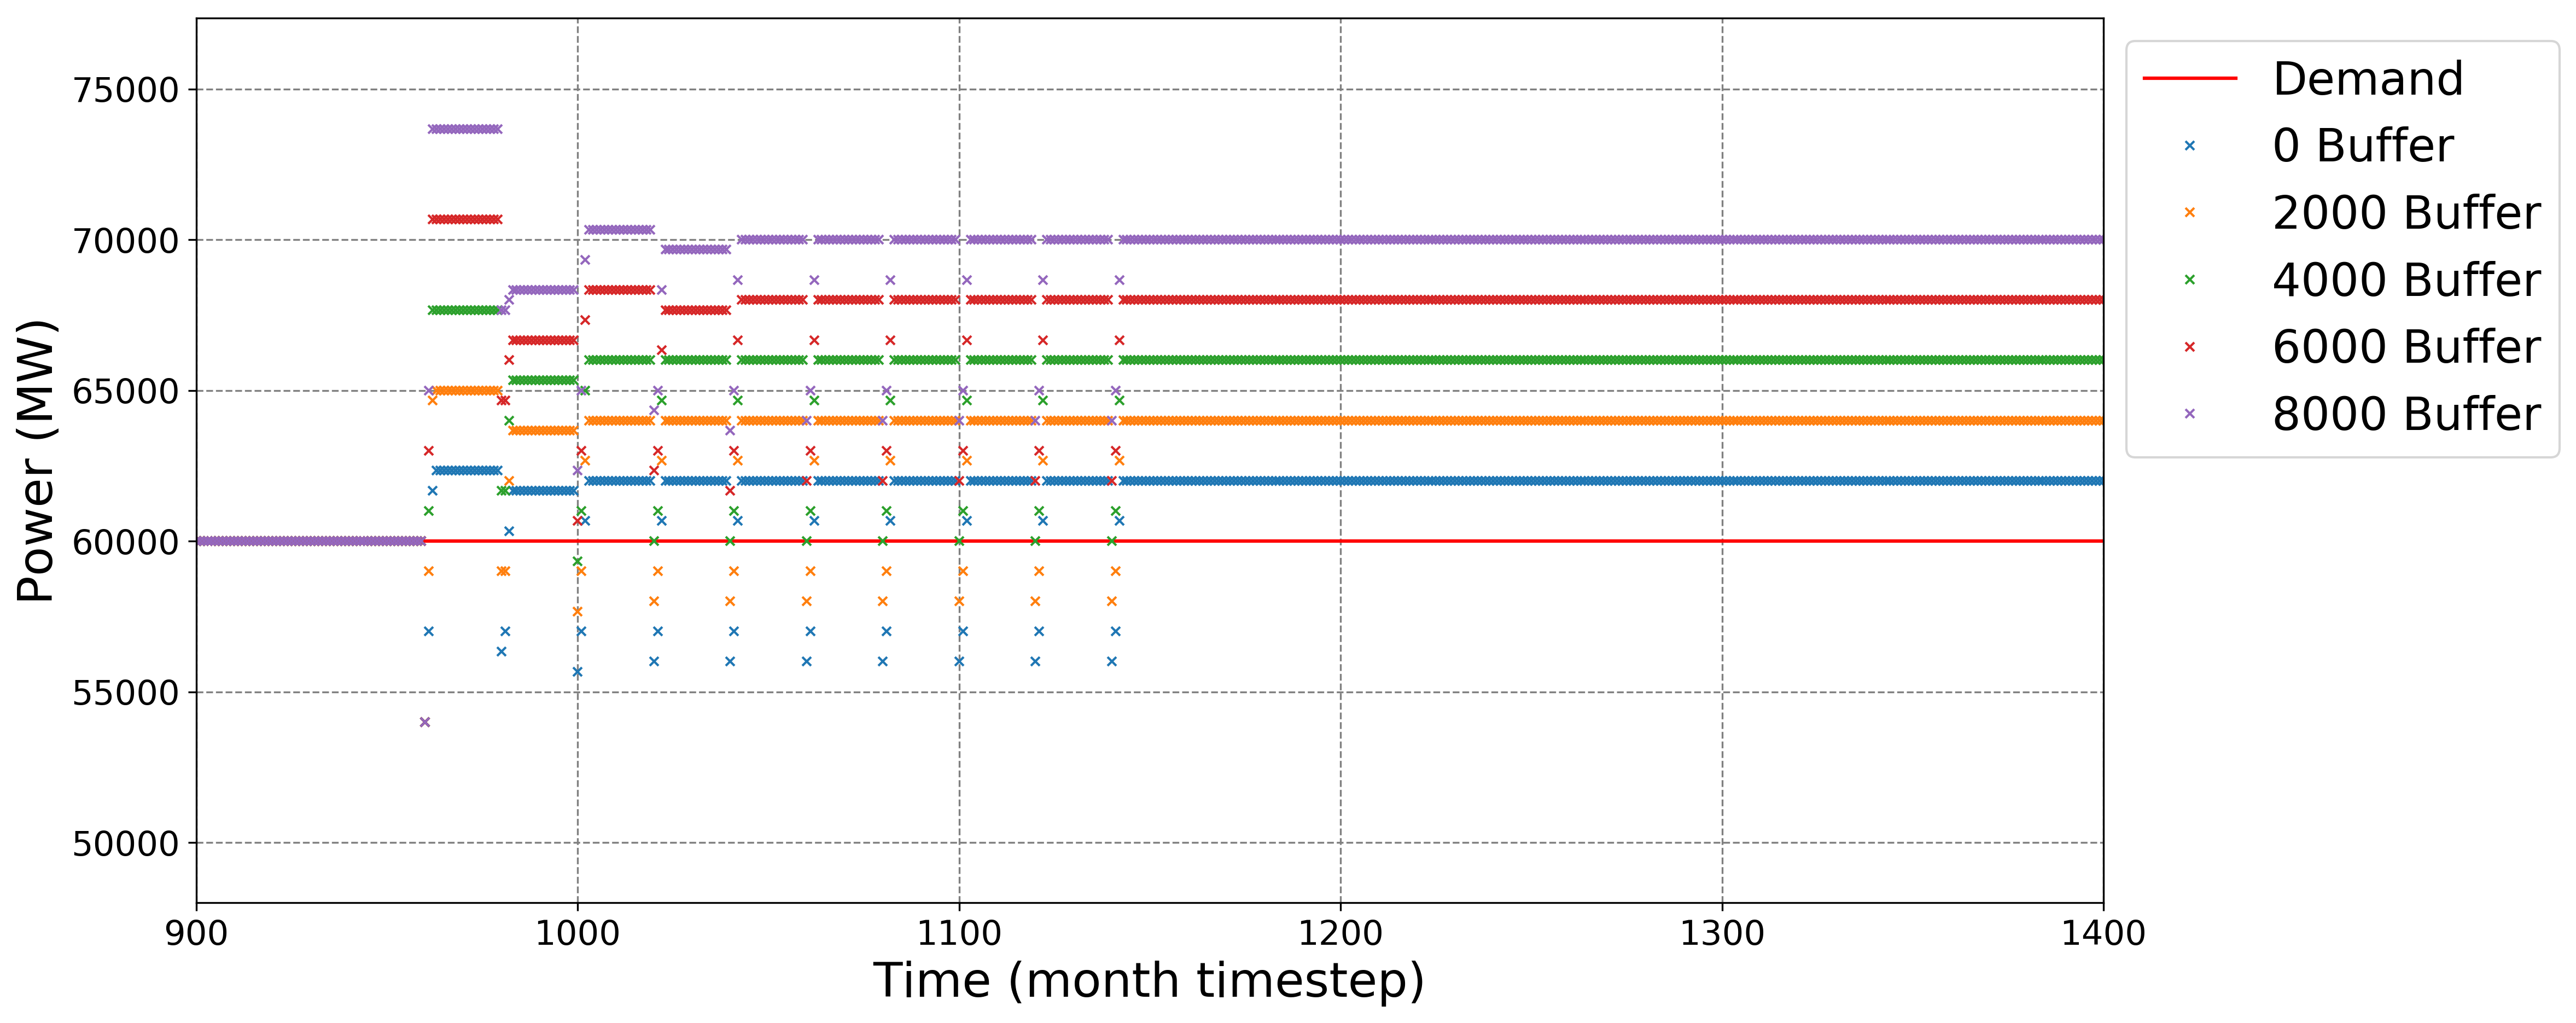
\includegraphics[width=\textwidth]{23-figures/23-power-buffer-arch.png} 
	\hfill
    \caption{Power supply for different buffer sizes using arch.}
	\label{fig:23-buf-arch}
\end{figure}

\begin{figure}[H]
	\centering
	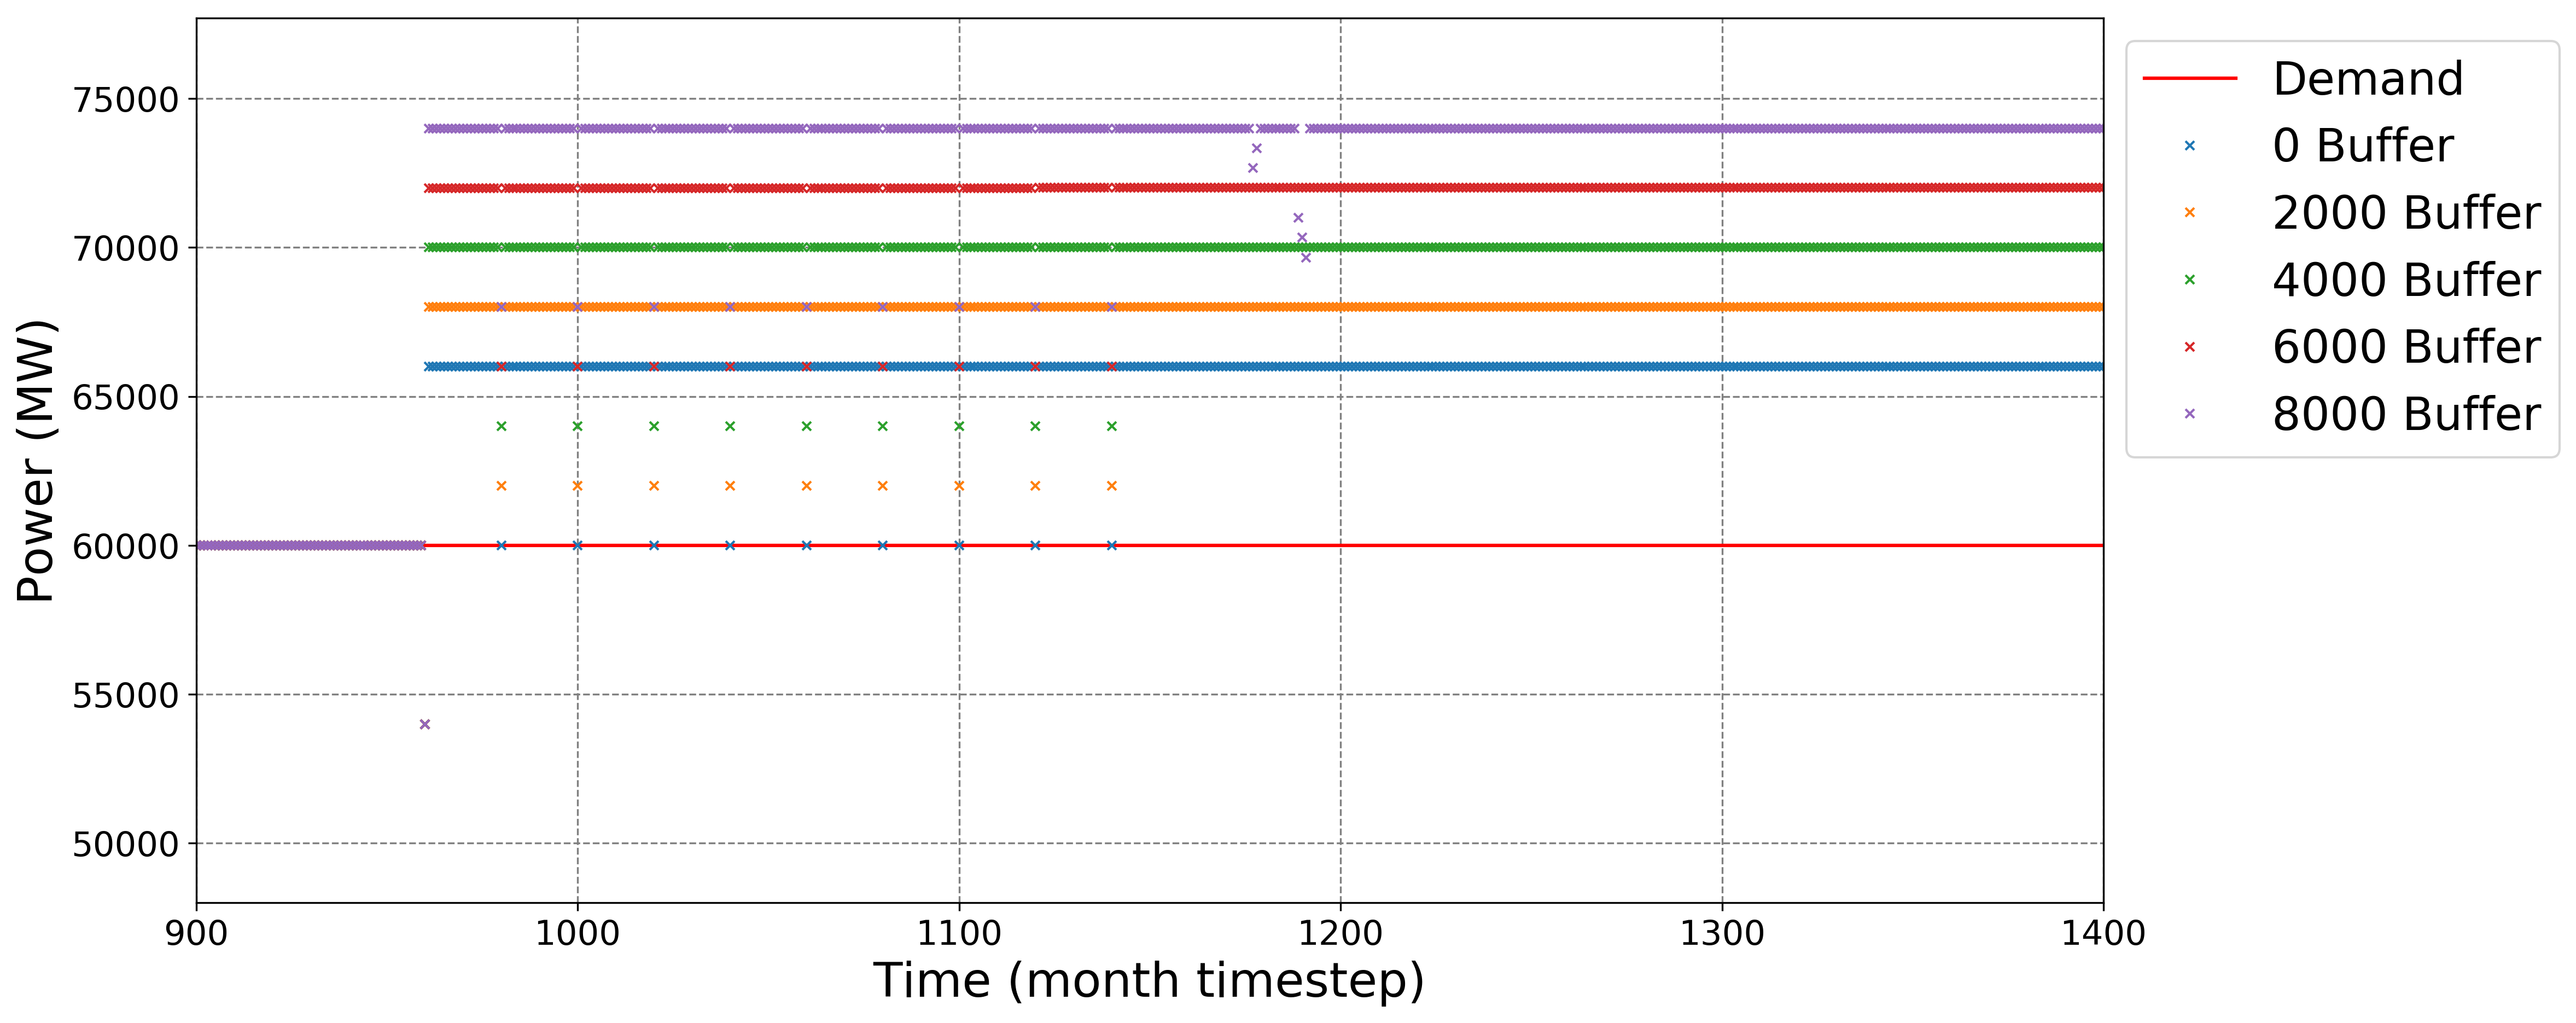
\includegraphics[width=\textwidth]{23-figures/23-power-buffer-poly.png} 
	\hfill
    \caption{Power supply for different buffer sizes using poly.}
	\label{fig:23-buf-poly}
\end{figure}

\begin{figure}[H]
	\centering
	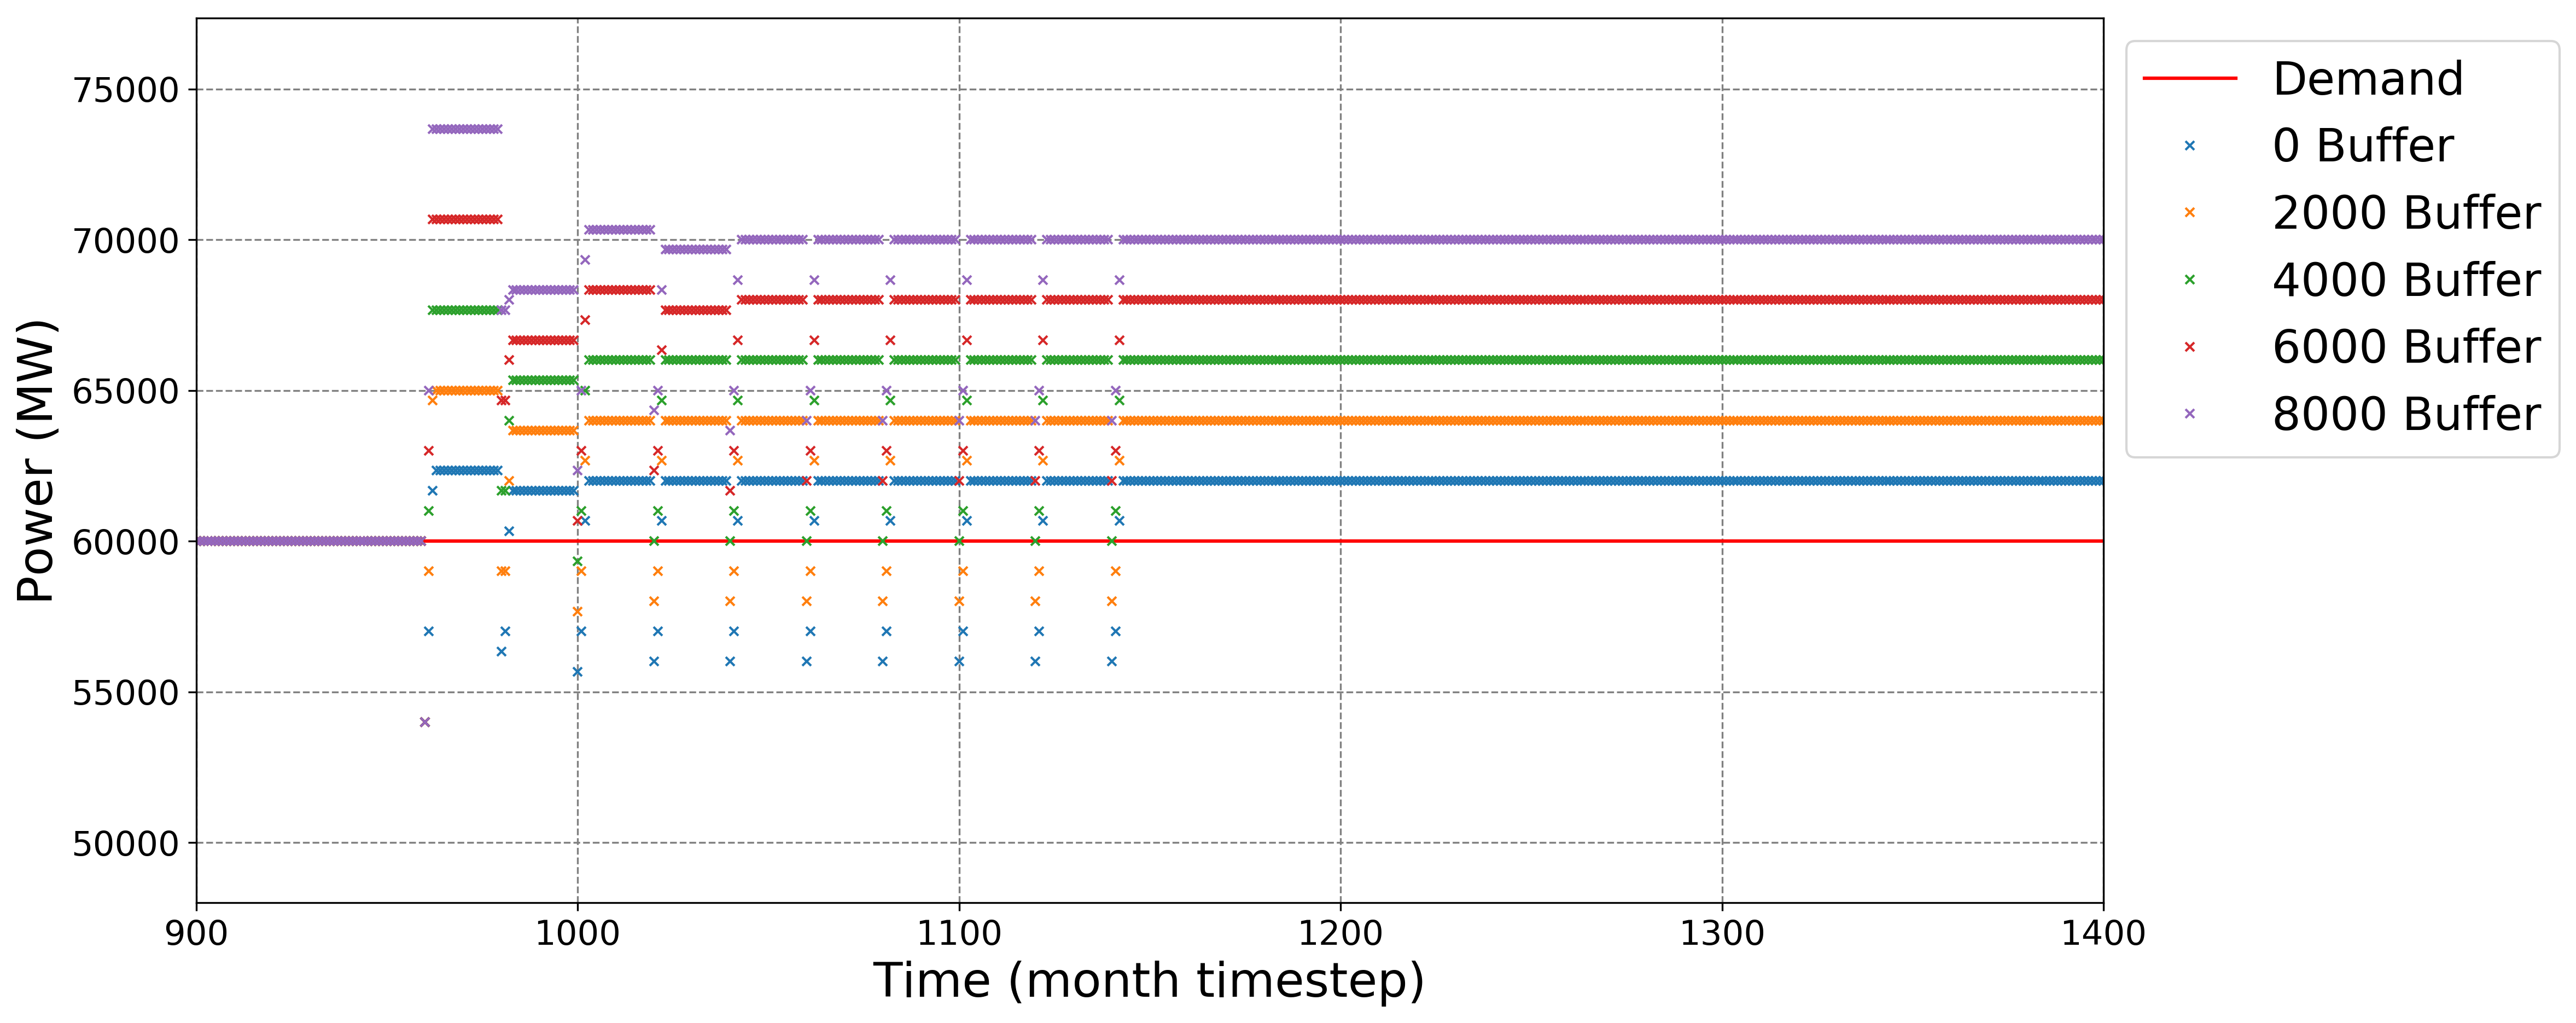
\includegraphics[width=\textwidth]{23-figures/23-power-buffer-exp_smoothing.png} 
	\hfill
    \caption{Power supply for different buffer sizes using exp\_smoothing.}
	\label{fig:23-buf-exp_smoothing}
\end{figure}

\begin{figure}[H]
	\centering
	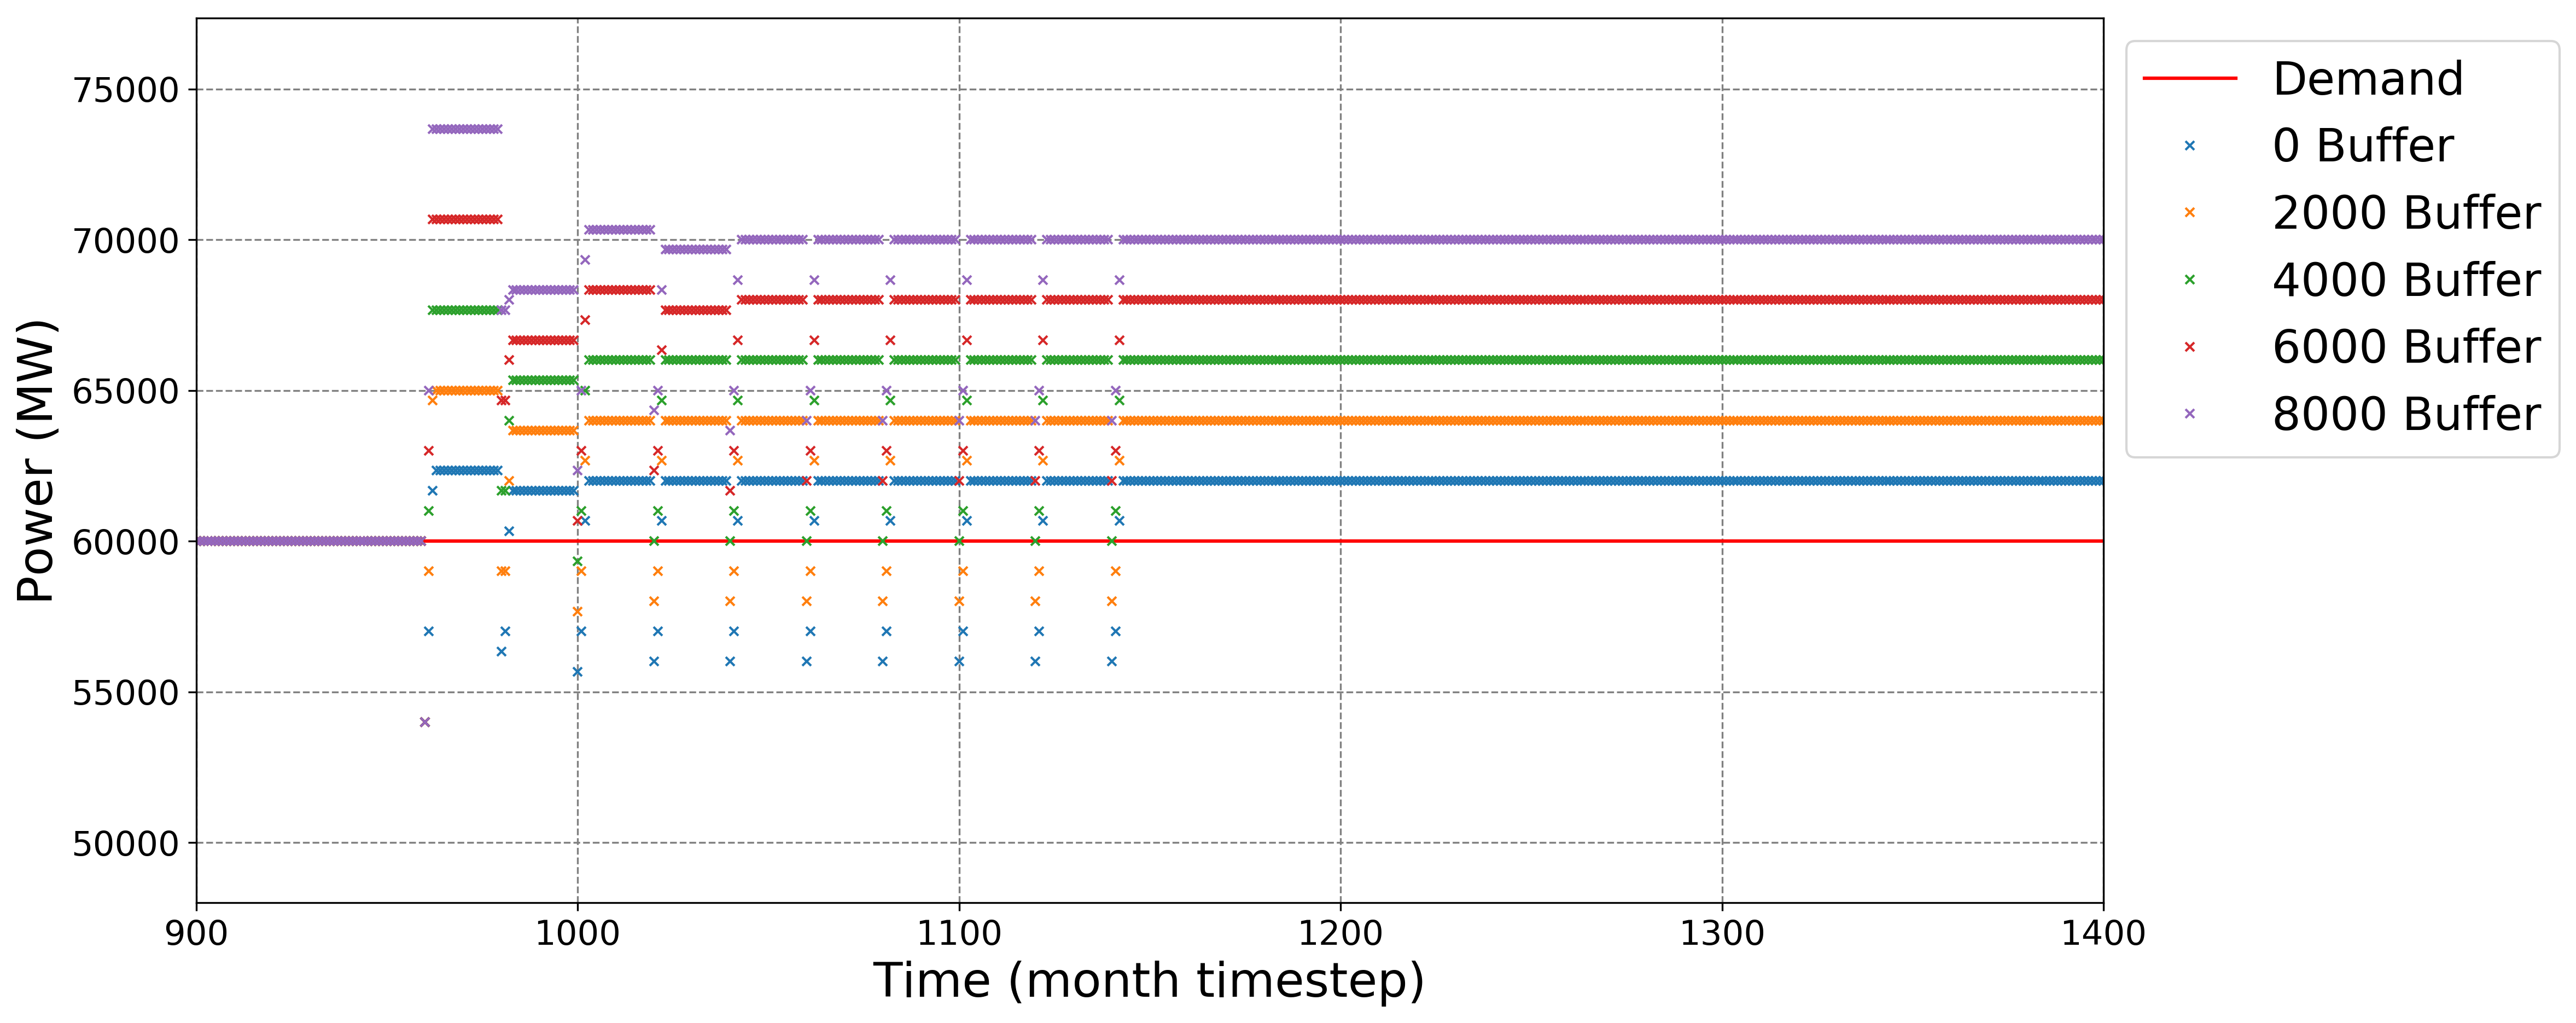
\includegraphics[width=\textwidth]{23-figures/23-power-buffer-holt_winters.png} 
	\hfill
	\caption{Power supply for different buffer sizes using holt\_winters.}
	\label{fig:23-buf-hots_winters}
\end{figure}

\begin{figure}[H]
	\centering
	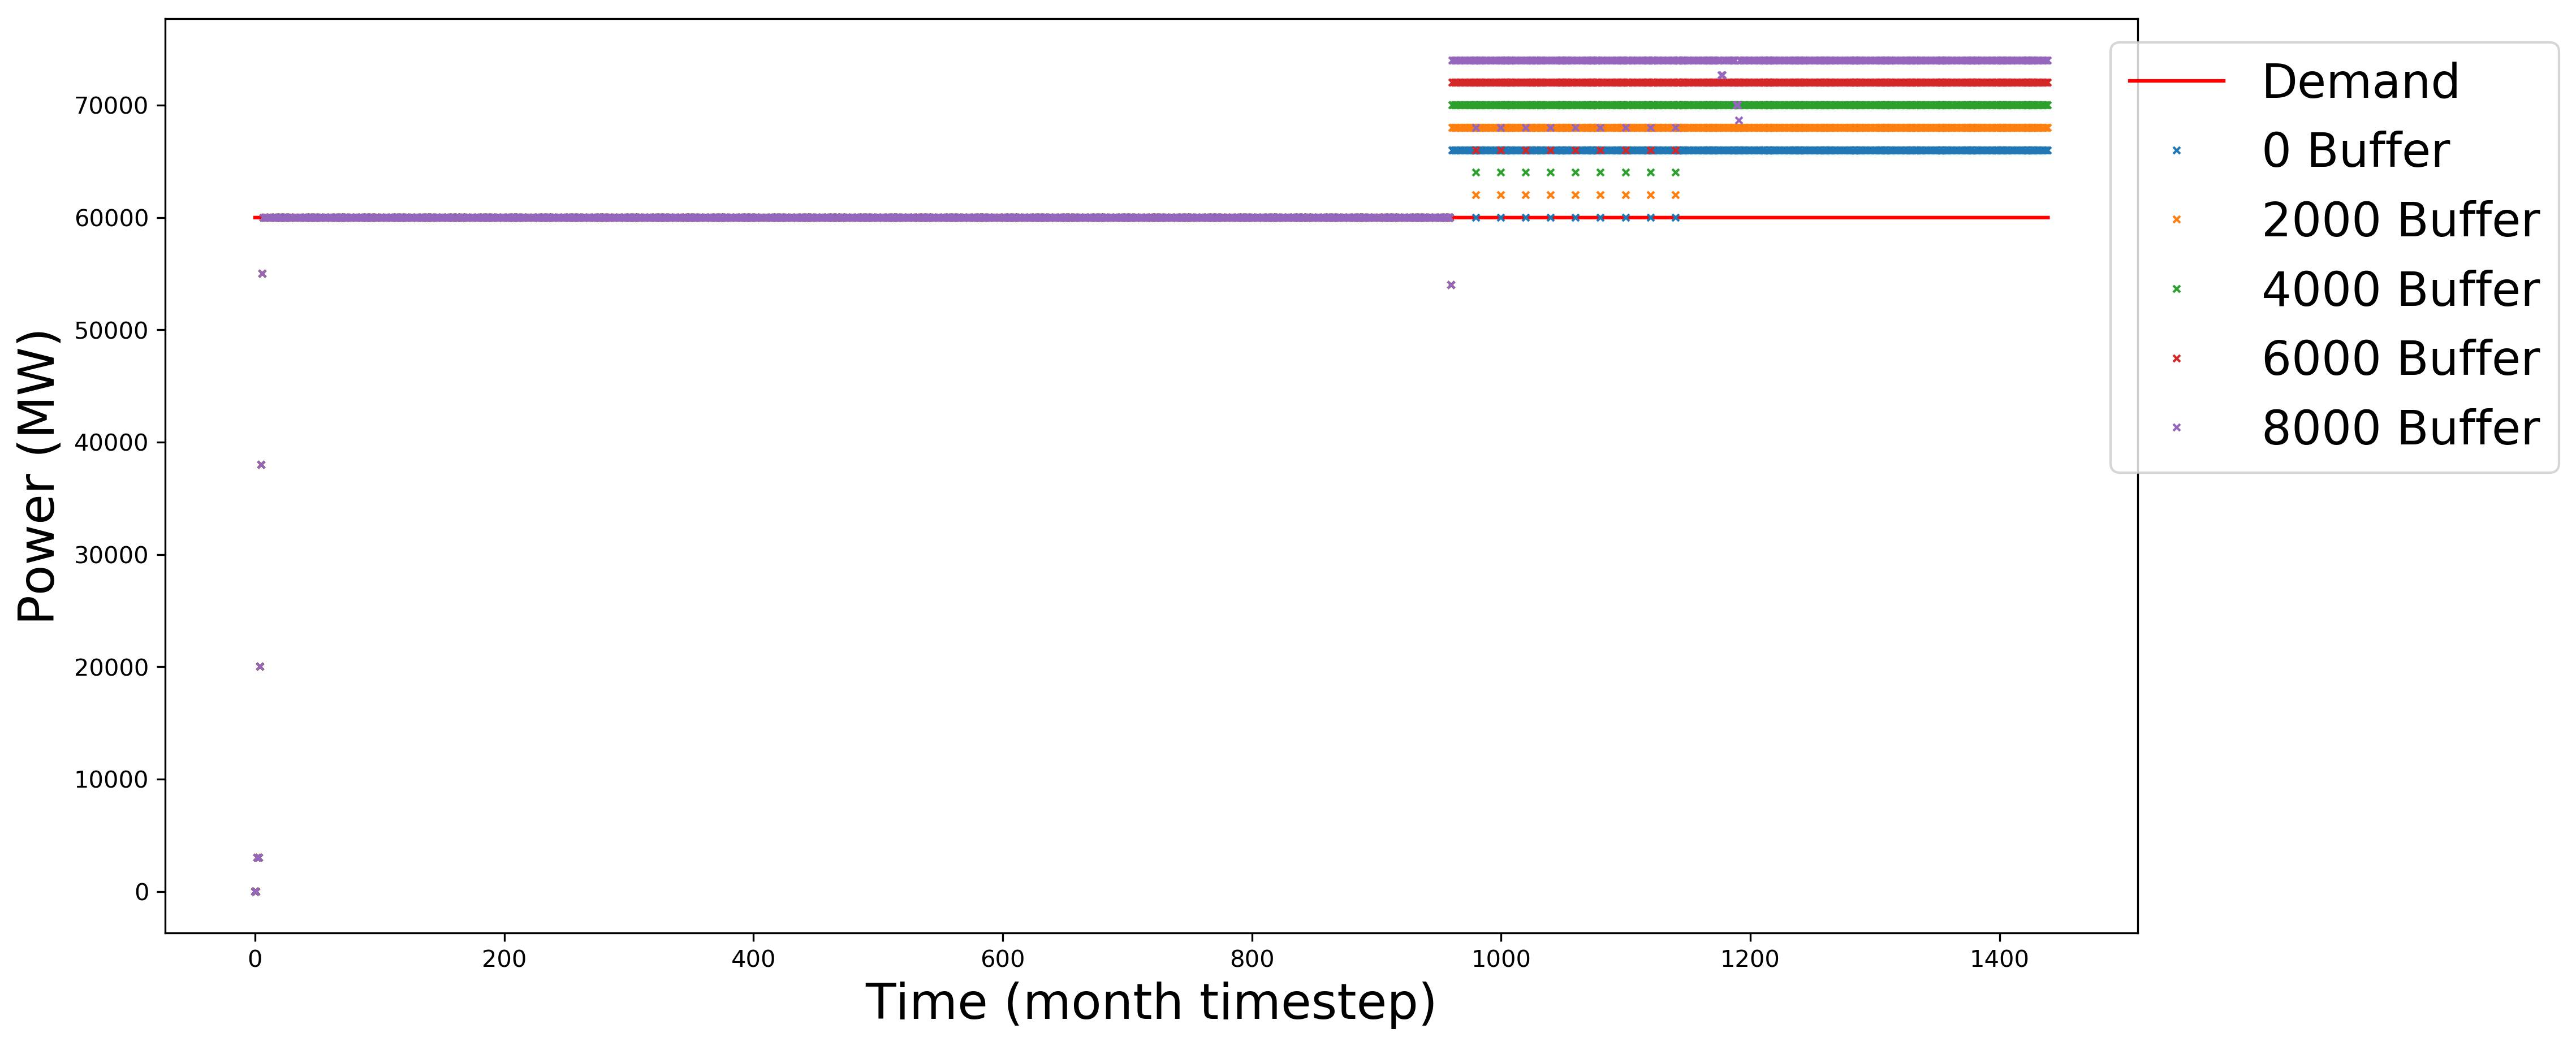
\includegraphics[width=\textwidth]{23-figures/23-power-buffer-fft.png} 
	\hfill
    \caption{Power supply for different buffer sizes using fft.}
	\label{fig:23-buf-fft}
\end{figure}

\subsection{Steps forward}

This section presents a sensitivity analysis for different values of steps.
Figure \ref{fig:23-steps} shows a comparison of the cumulative under supply for different values of steps forward.

Figures \ref{fig:23-ste-ma} to \ref{fig:23-ste-fft} display a comparison for some of the methods of the power supply for different steps.

The input files use the installed capacity feature. Buffer is set to zero, back steps is set to two, and steps takes the values 1, 2, 3, 4, and 5.

Seeing figure \ref{fig:23-steps} we note that the more steps used, the worse the simulation performs. Figure \ref{fig:23-ste-fft-mixerout} helps to understand such behavior. 'Mixerout' is the commodity that represents the fuel that FR use. This figure shows that the LWRs produce enough fuel to almost start all the FRs. However, this expense of fuel is too big to keep the ones already deployed running until they produce their own fuel, so their power supply oscillates. The steps capability should be used cautiously to avoid this from happening.

\begin{figure}[H]
	\centering
	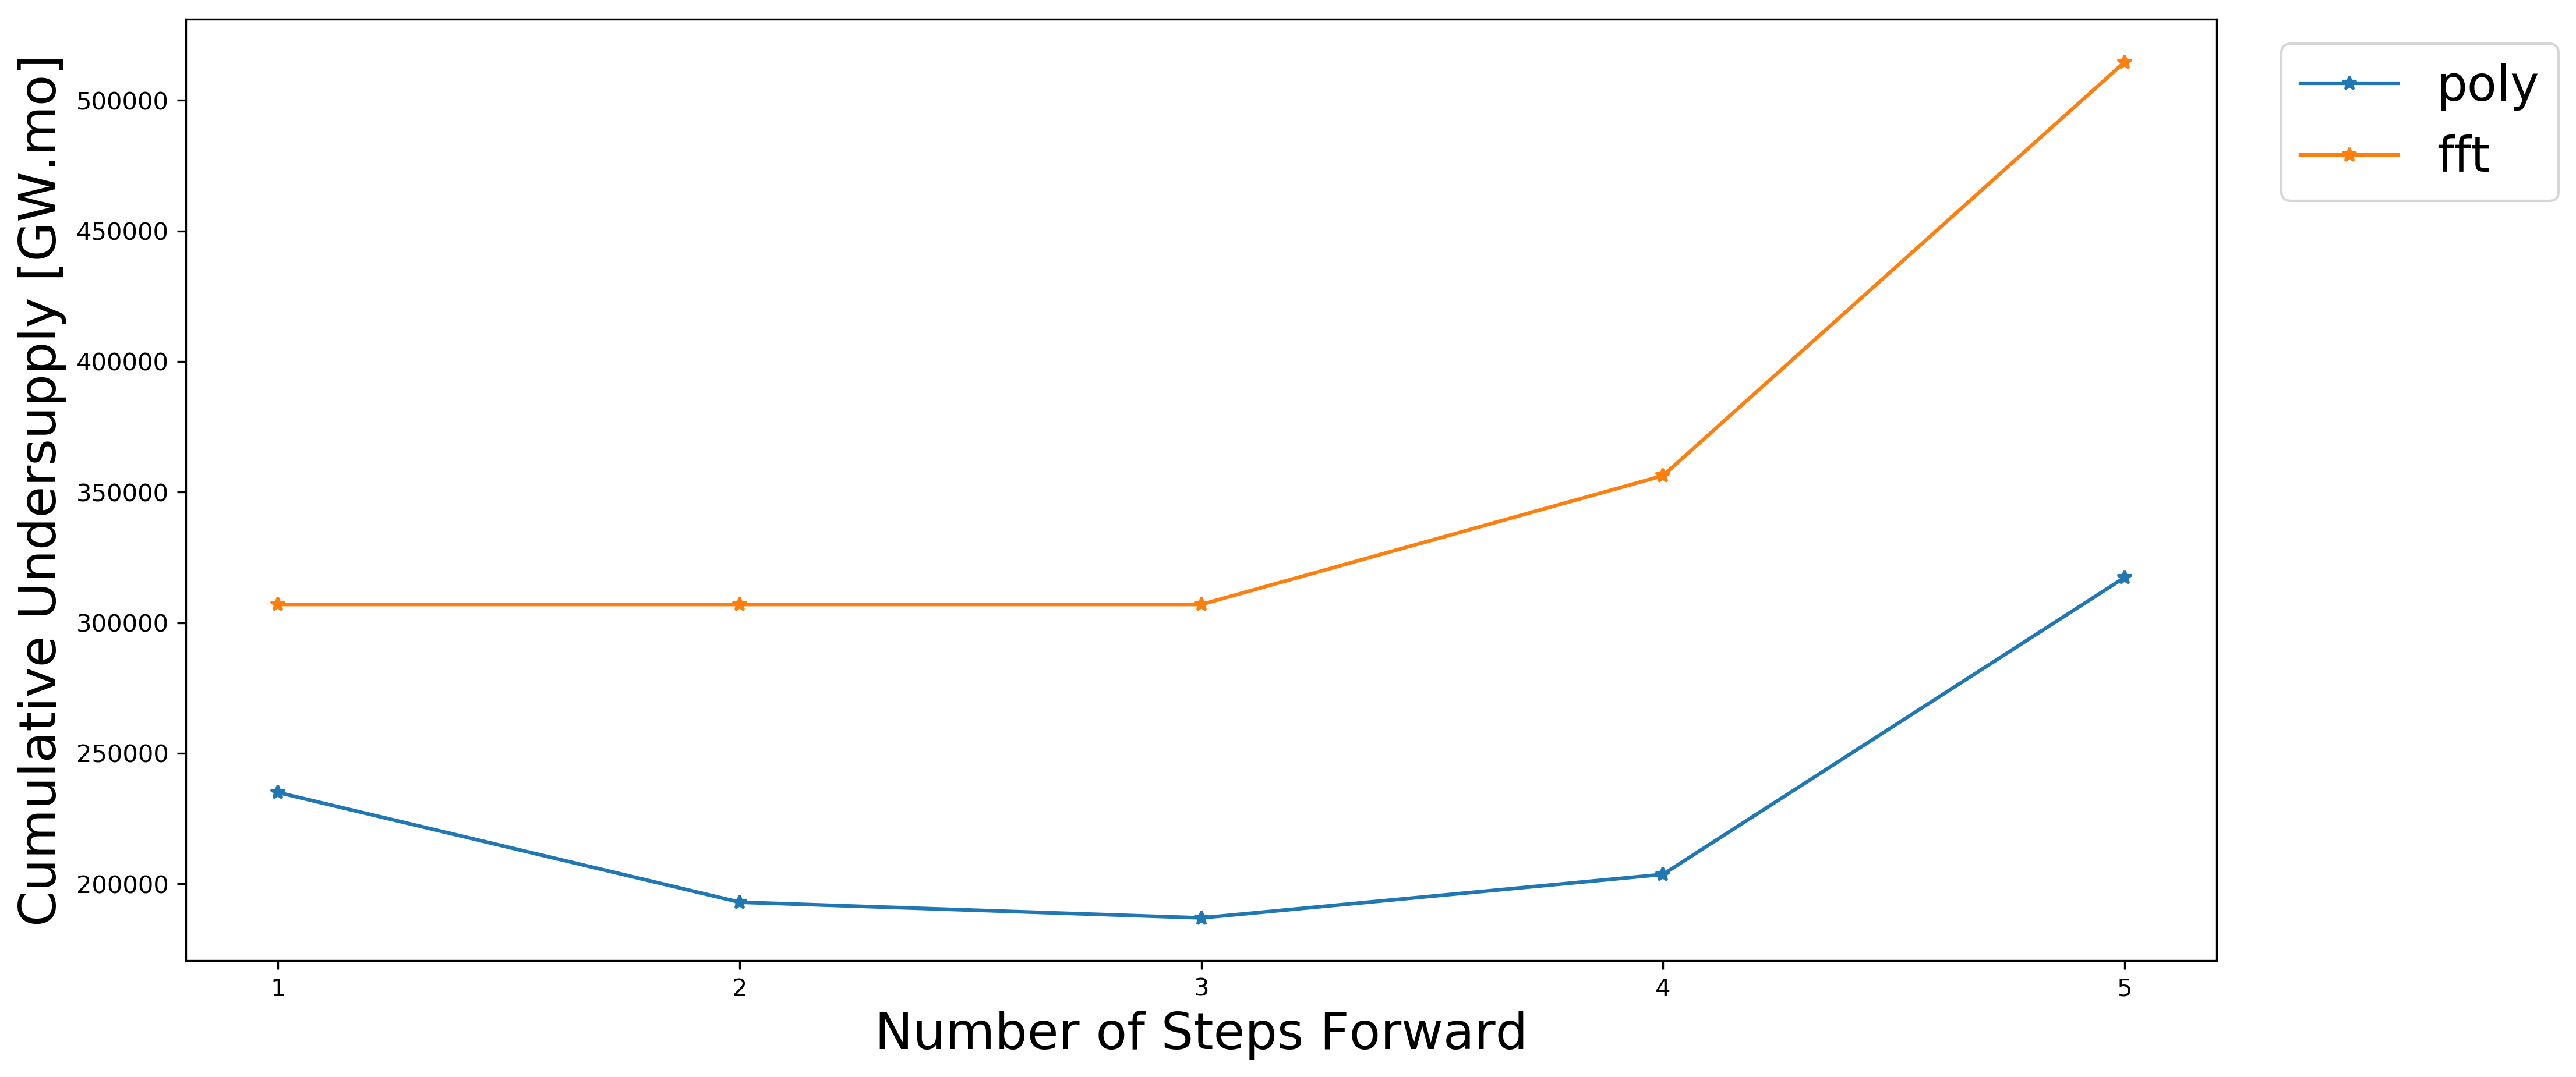
\includegraphics[width=\textwidth]{23-figures/23-sens-steps.png} 
	\hfill
	\caption{Sensitivity analysis for different number of steps forward for some prediction algorithms.}
	\label{fig:23-steps}
\end{figure}

\begin{figure}[H]
	\centering
	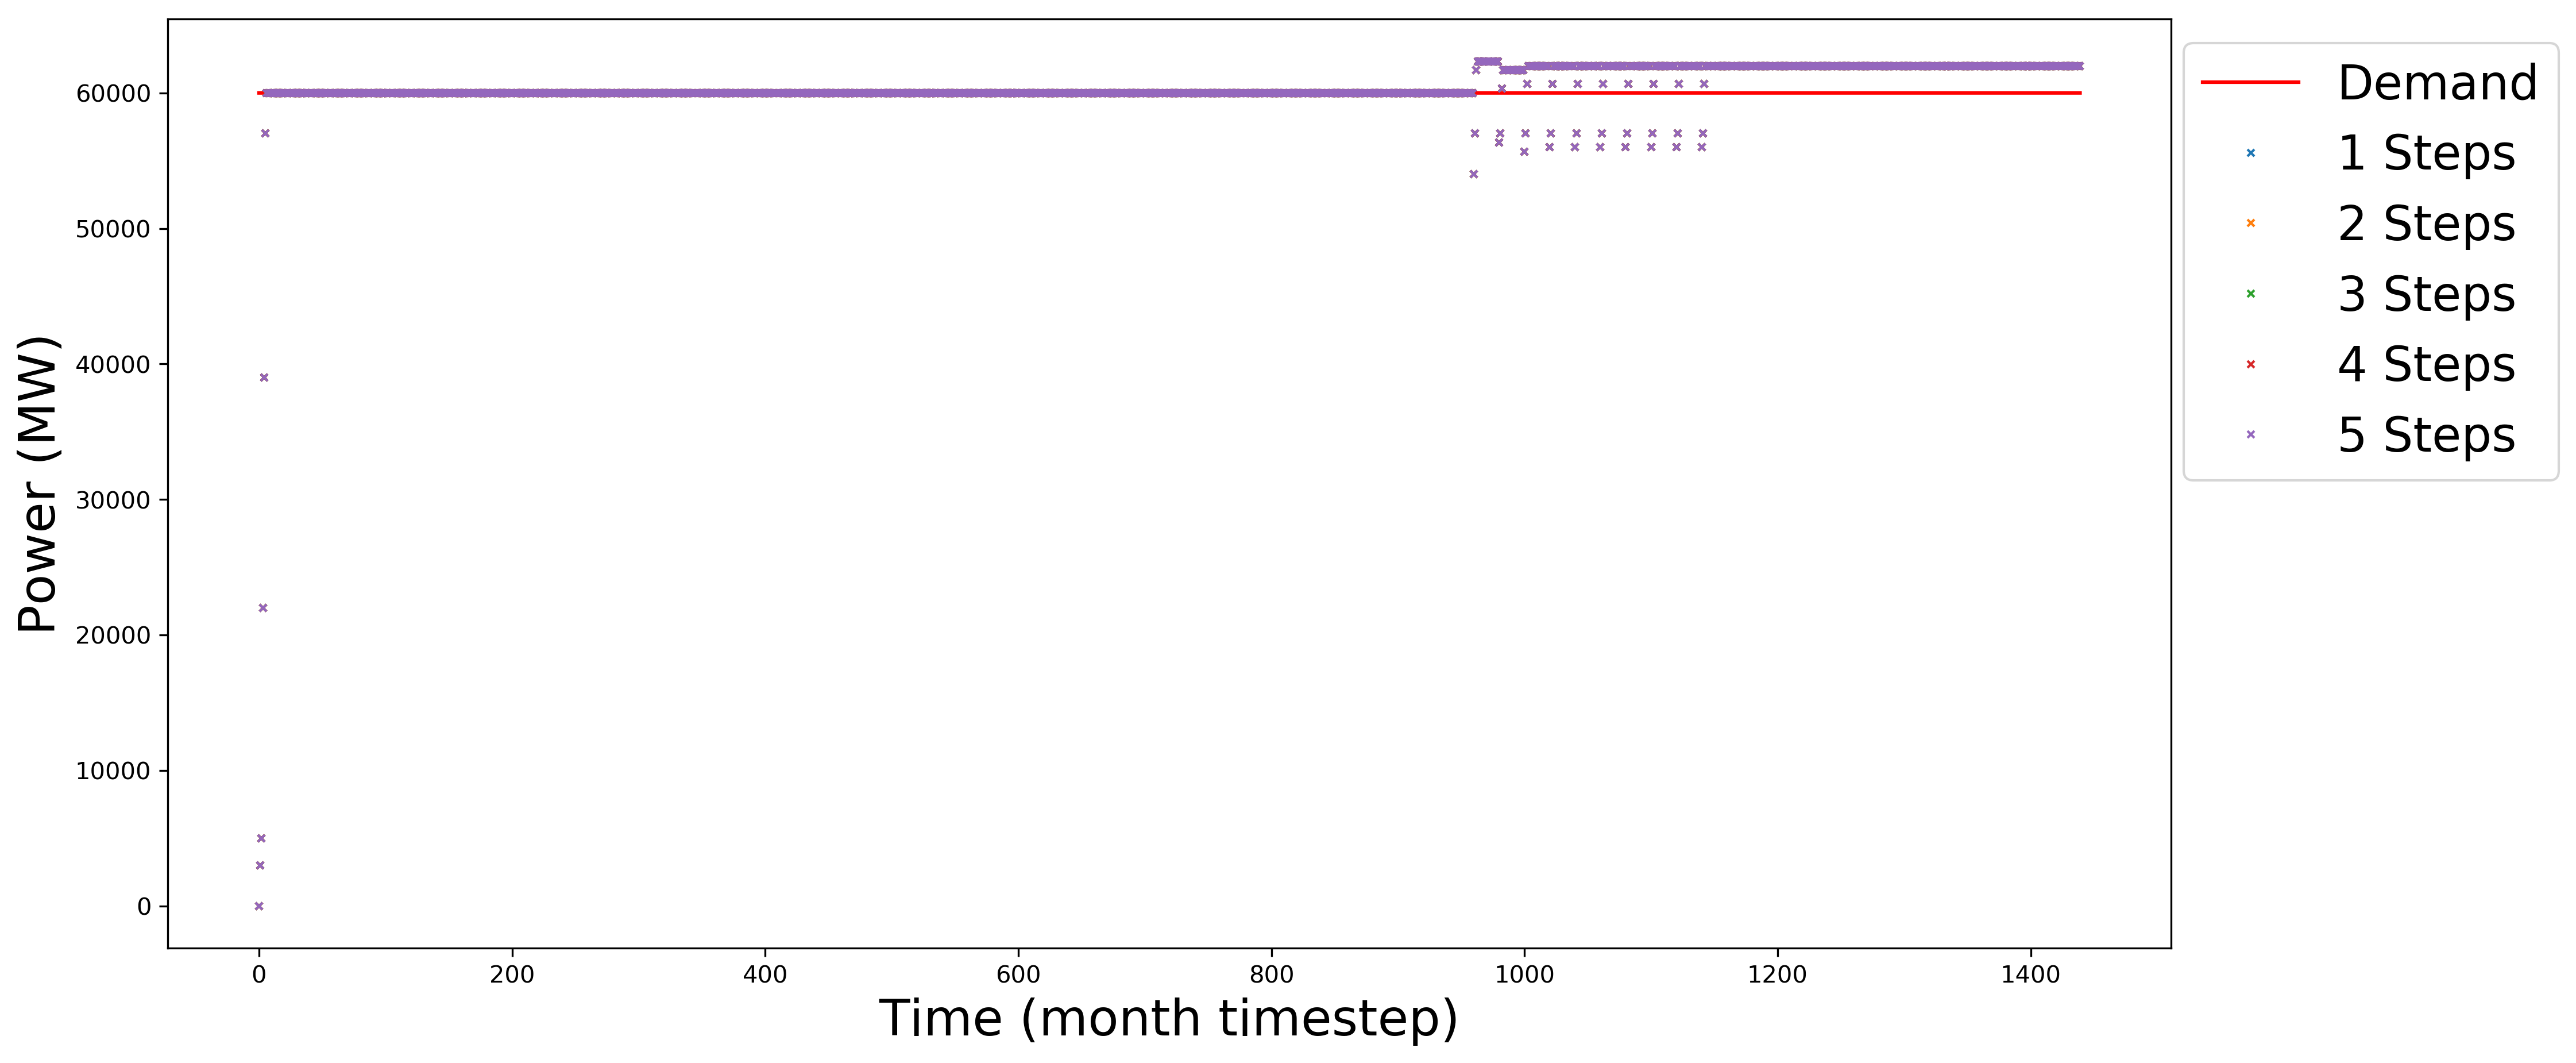
\includegraphics[width=\textwidth]{23-figures/23-power-buffer0-ma-steps.png} 
	\hfill
	\caption{Power supply for different values of steps forward using ma.}
	\label{fig:23-ste-ma}
\end{figure}

\begin{figure}[H]
	\centering
	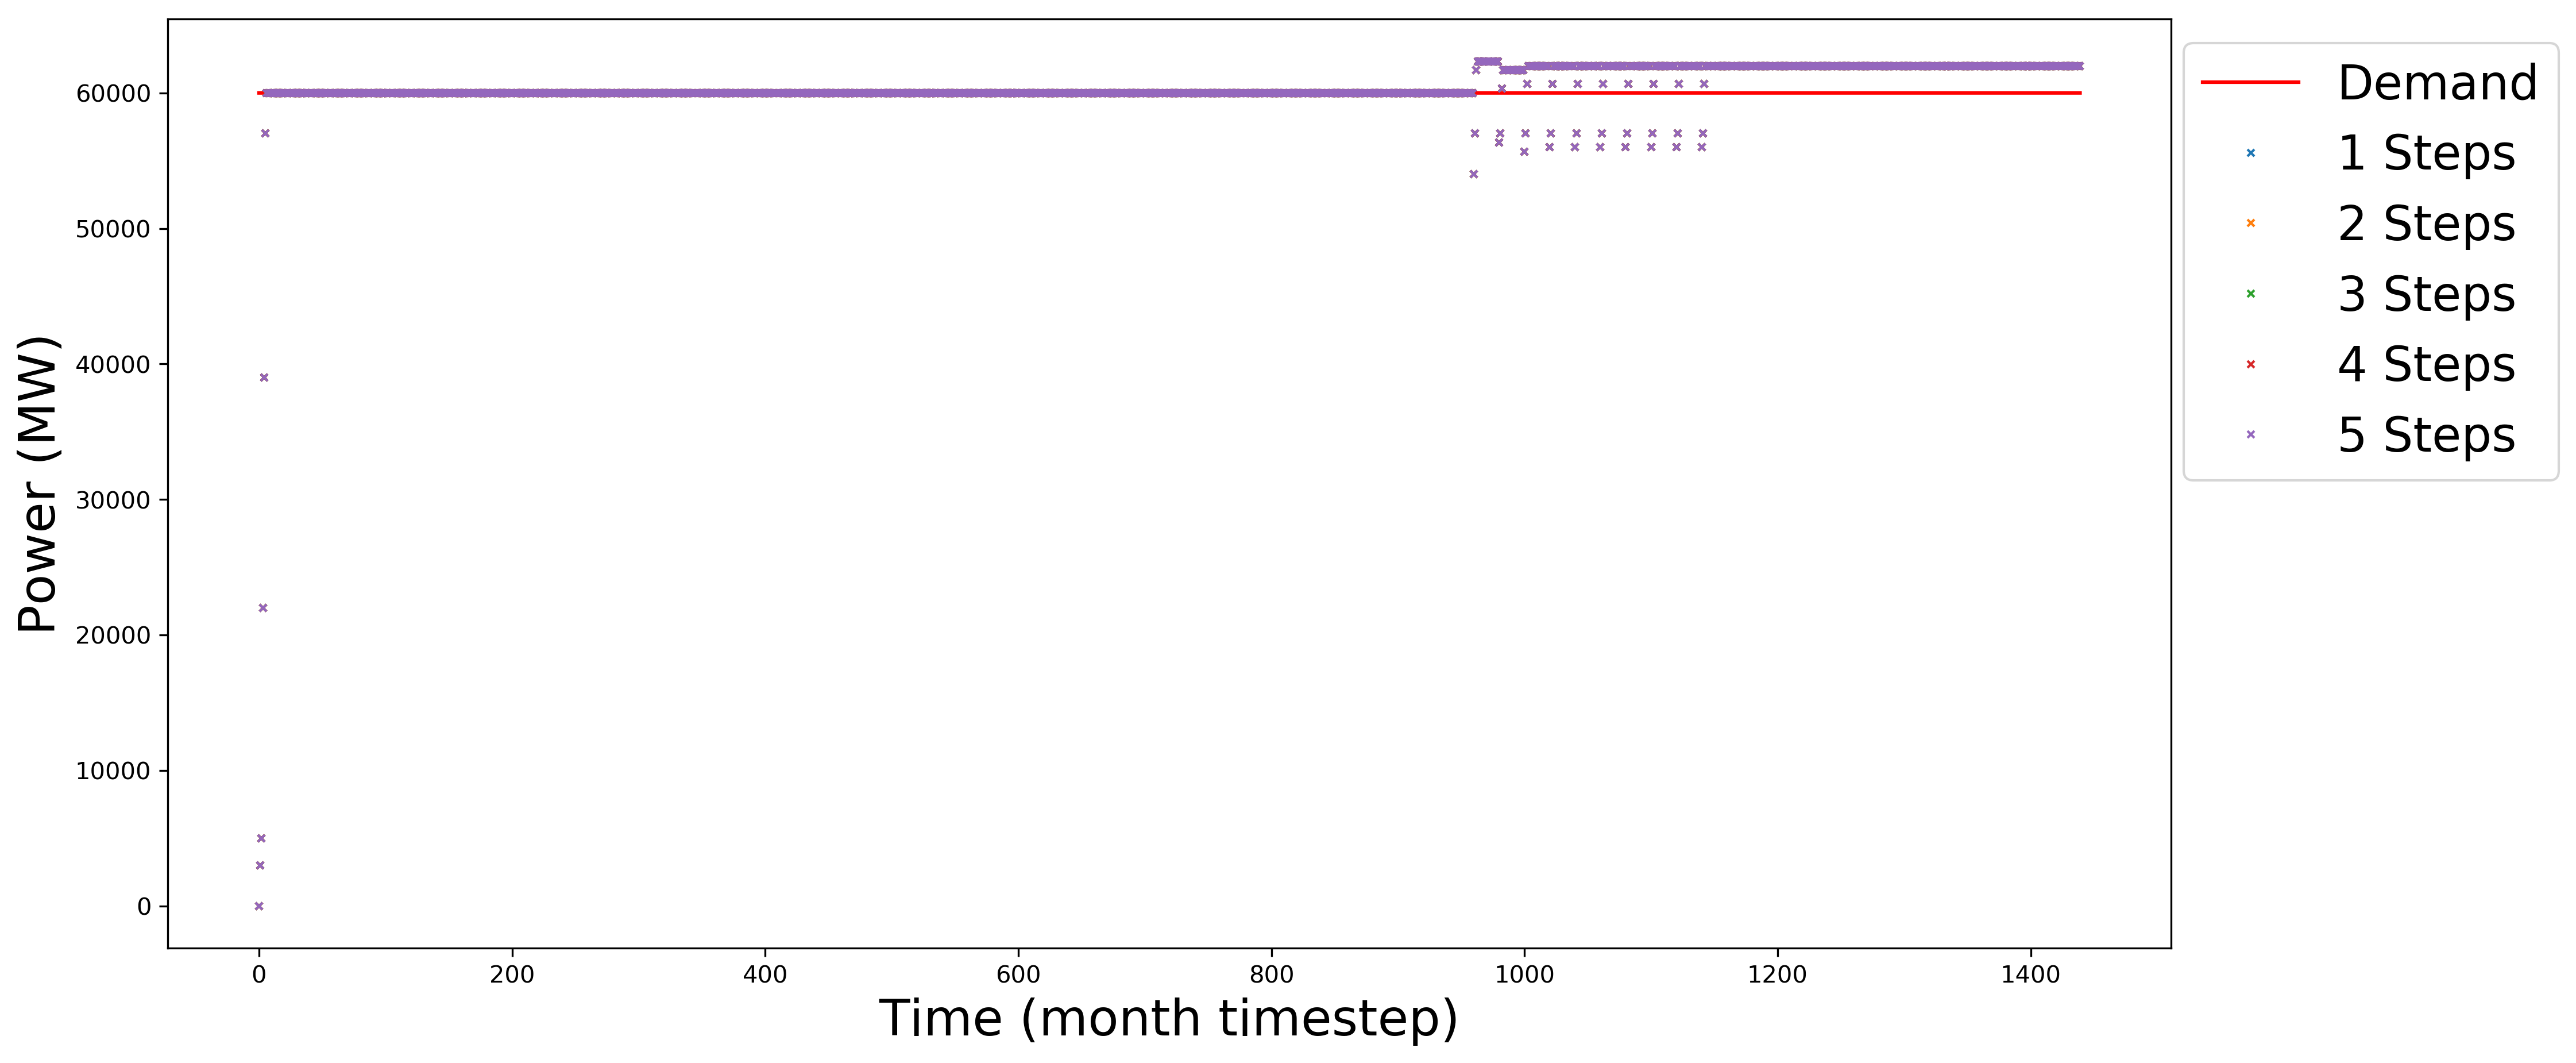
\includegraphics[width=\textwidth]{23-figures/23-power-buffer0-arma-steps.png} 
	\hfill
	\caption{Power supply for different values of steps forward using arma.}
	\label{fig:23-ste-arma}
\end{figure}

\begin{figure}[H]
	\centering
	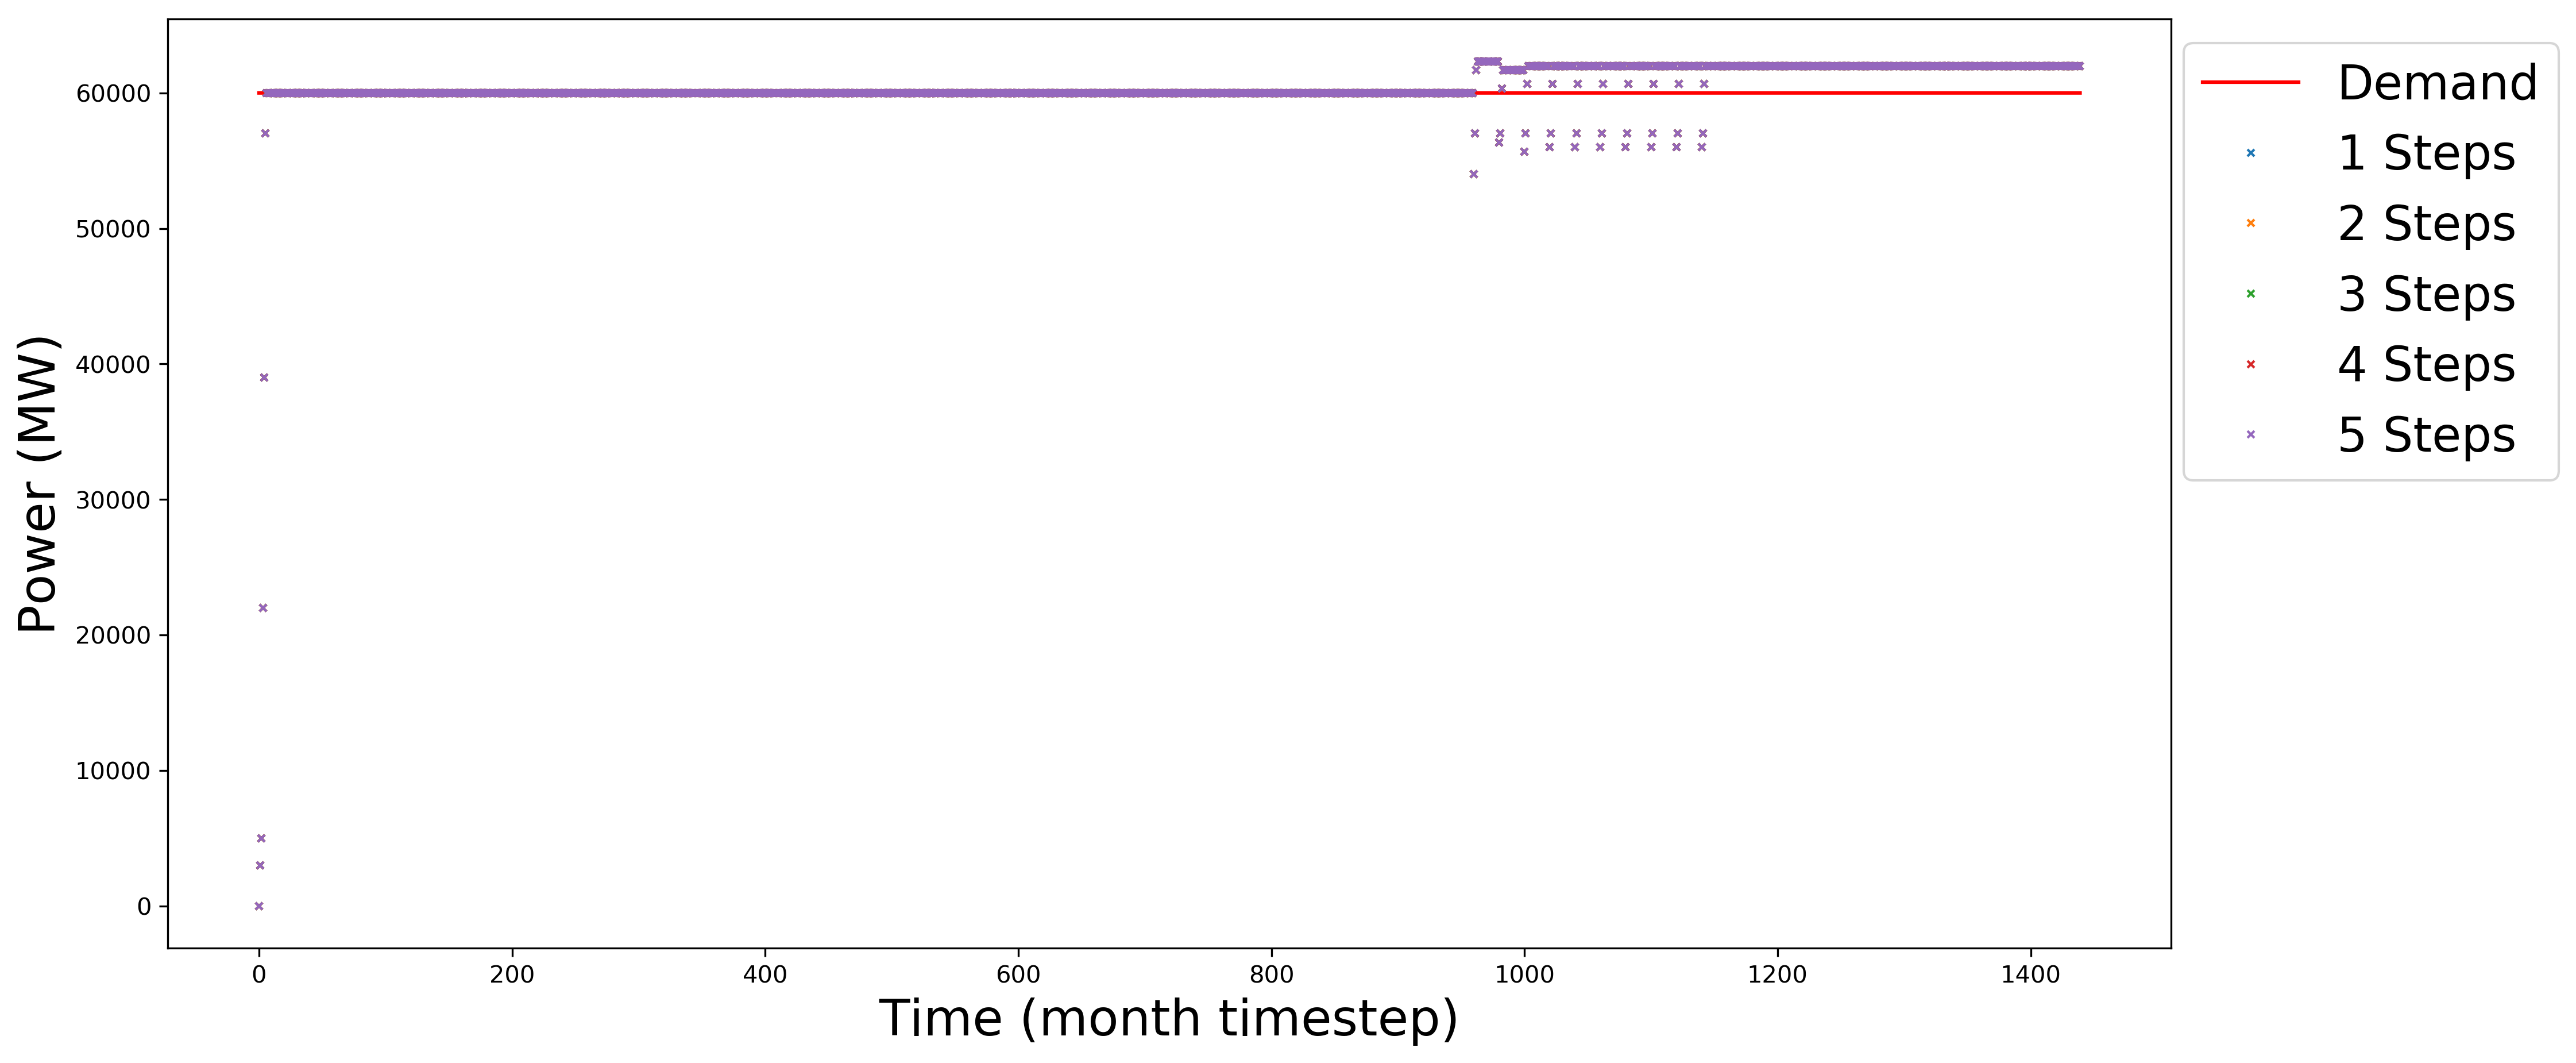
\includegraphics[width=\textwidth]{23-figures/23-power-buffer0-arch-steps.png} 
	\hfill
	\caption{Power supply for different values of steps forward using arch.}
	\label{fig:23-ste-arch}
\end{figure}

\begin{figure}[H]
	\centering
	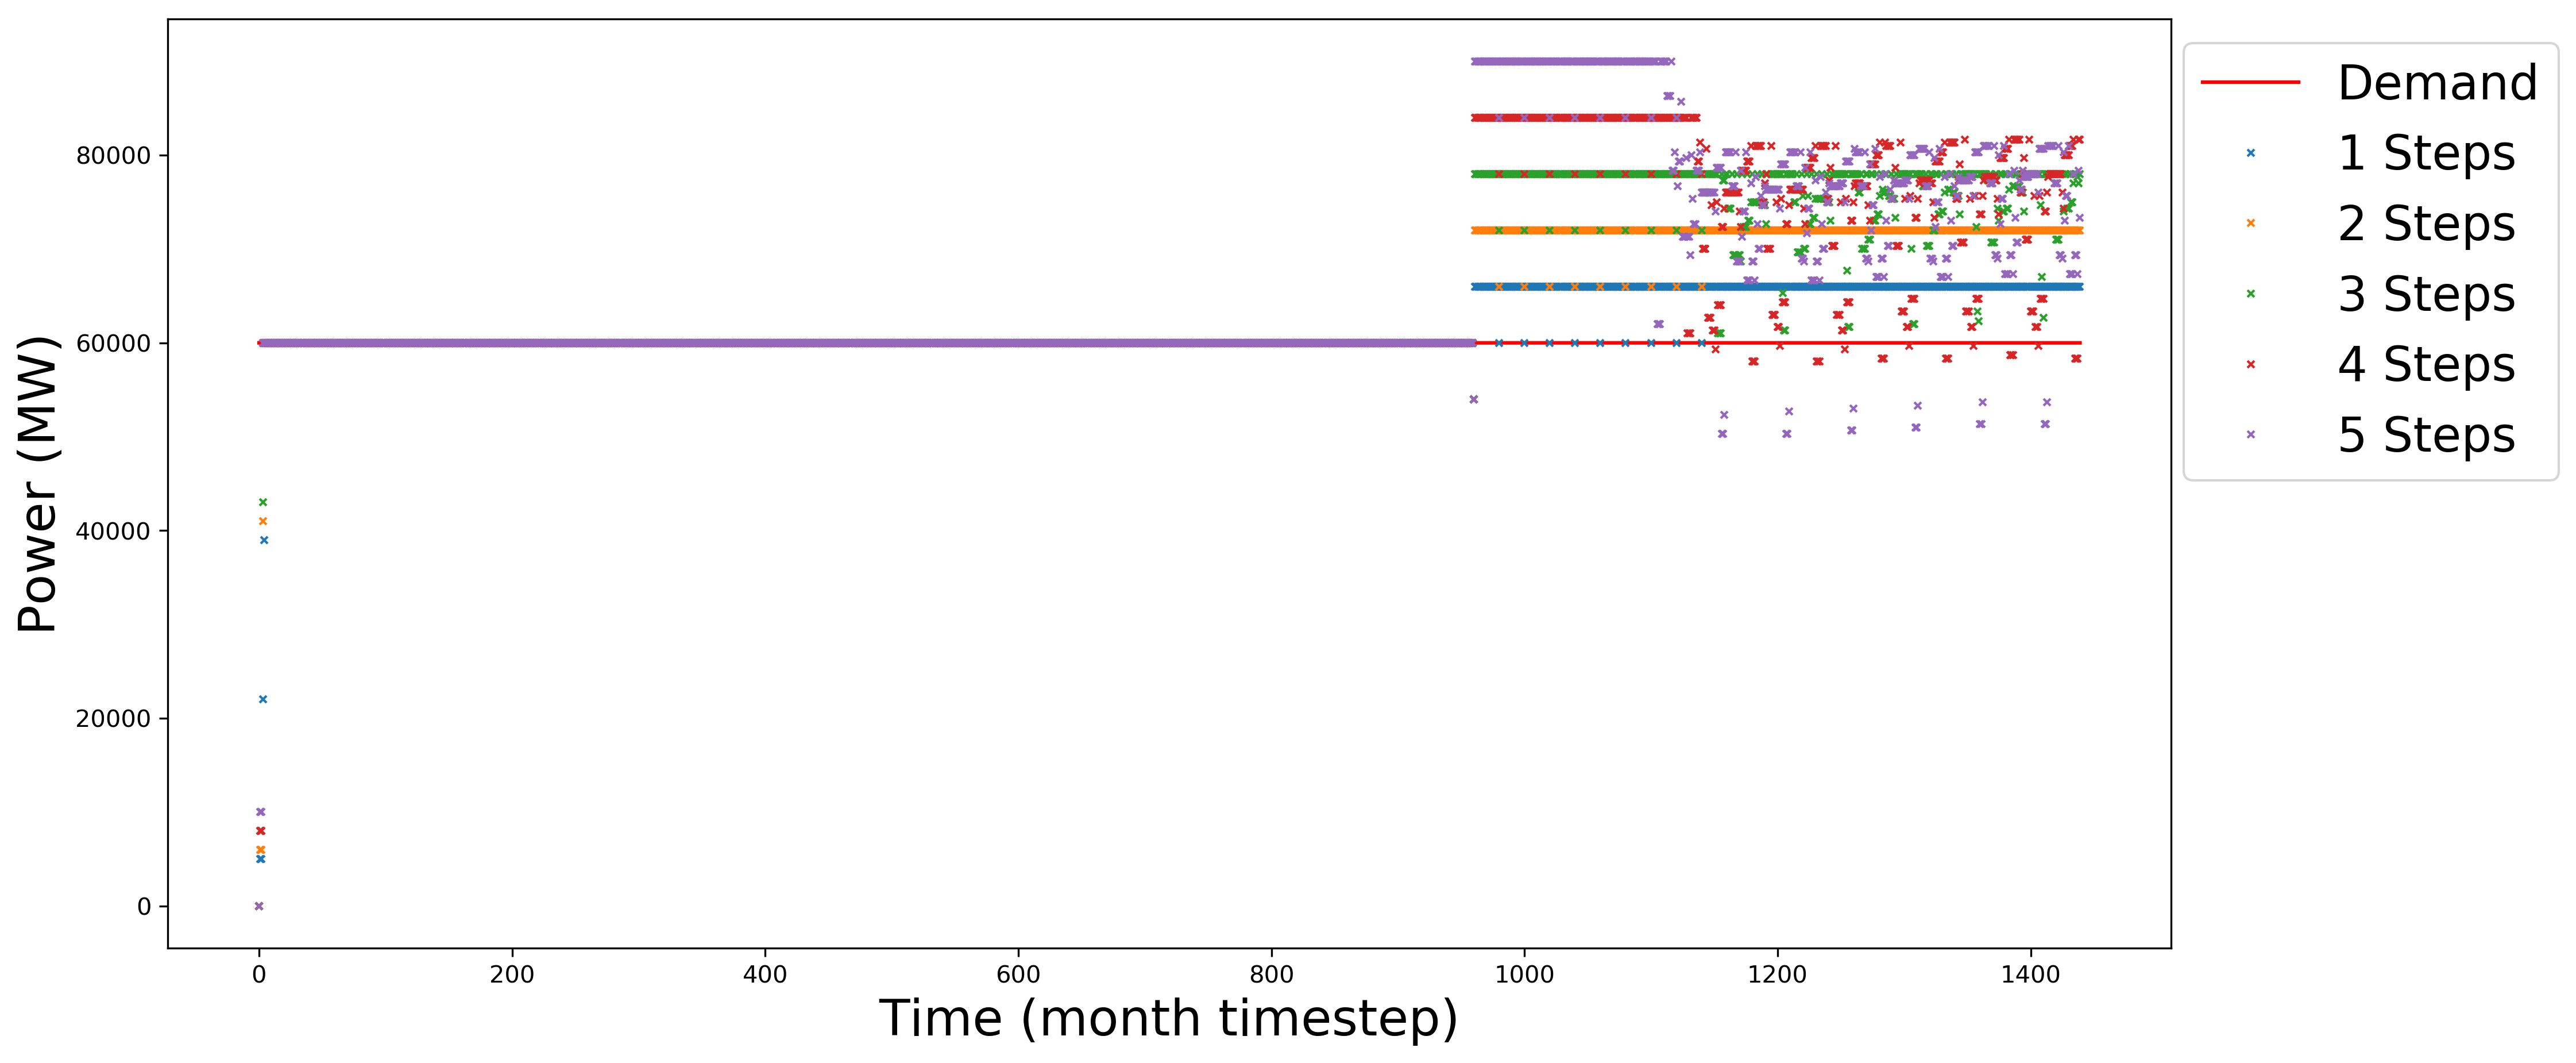
\includegraphics[width=\textwidth]{23-figures/23-power-buffer0-poly-steps.png} 
	\hfill
	\caption{Power supply for different values of steps forward using poly.}
	\label{fig:23-ste-poly}
\end{figure}

\begin{figure}[H]
	\centering
	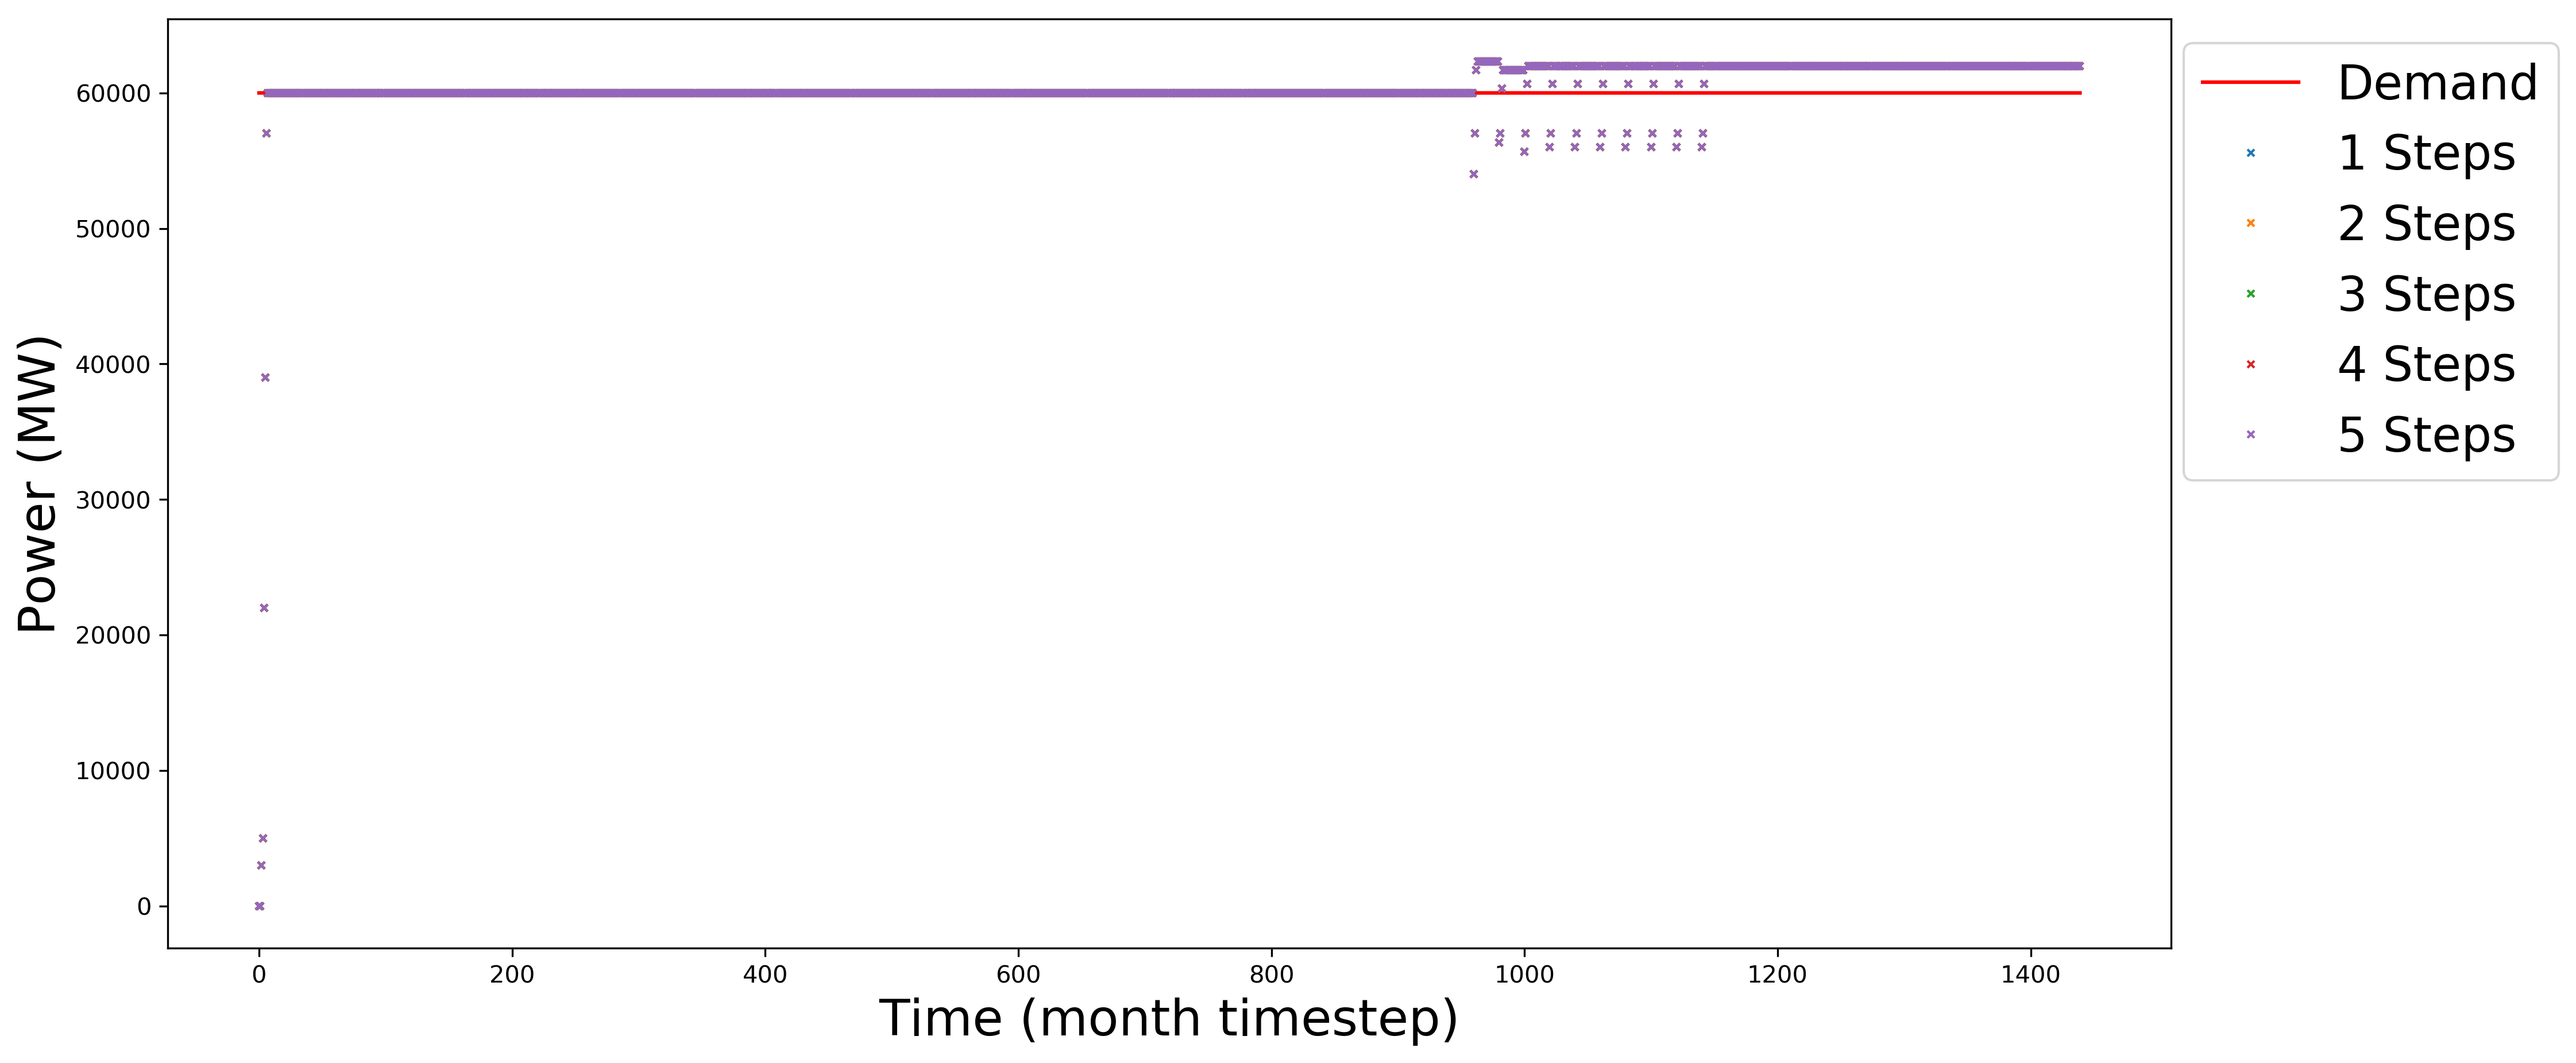
\includegraphics[width=\textwidth]{23-figures/23-power-buffer0-exp_smoothing-steps.png} 
	\hfill
	\caption{Power supply for different values of steps forward using exp\_smoothing.}
	\label{fig:23-ste-exp_smoothing}
\end{figure}

\begin{figure}[H]
	\centering
	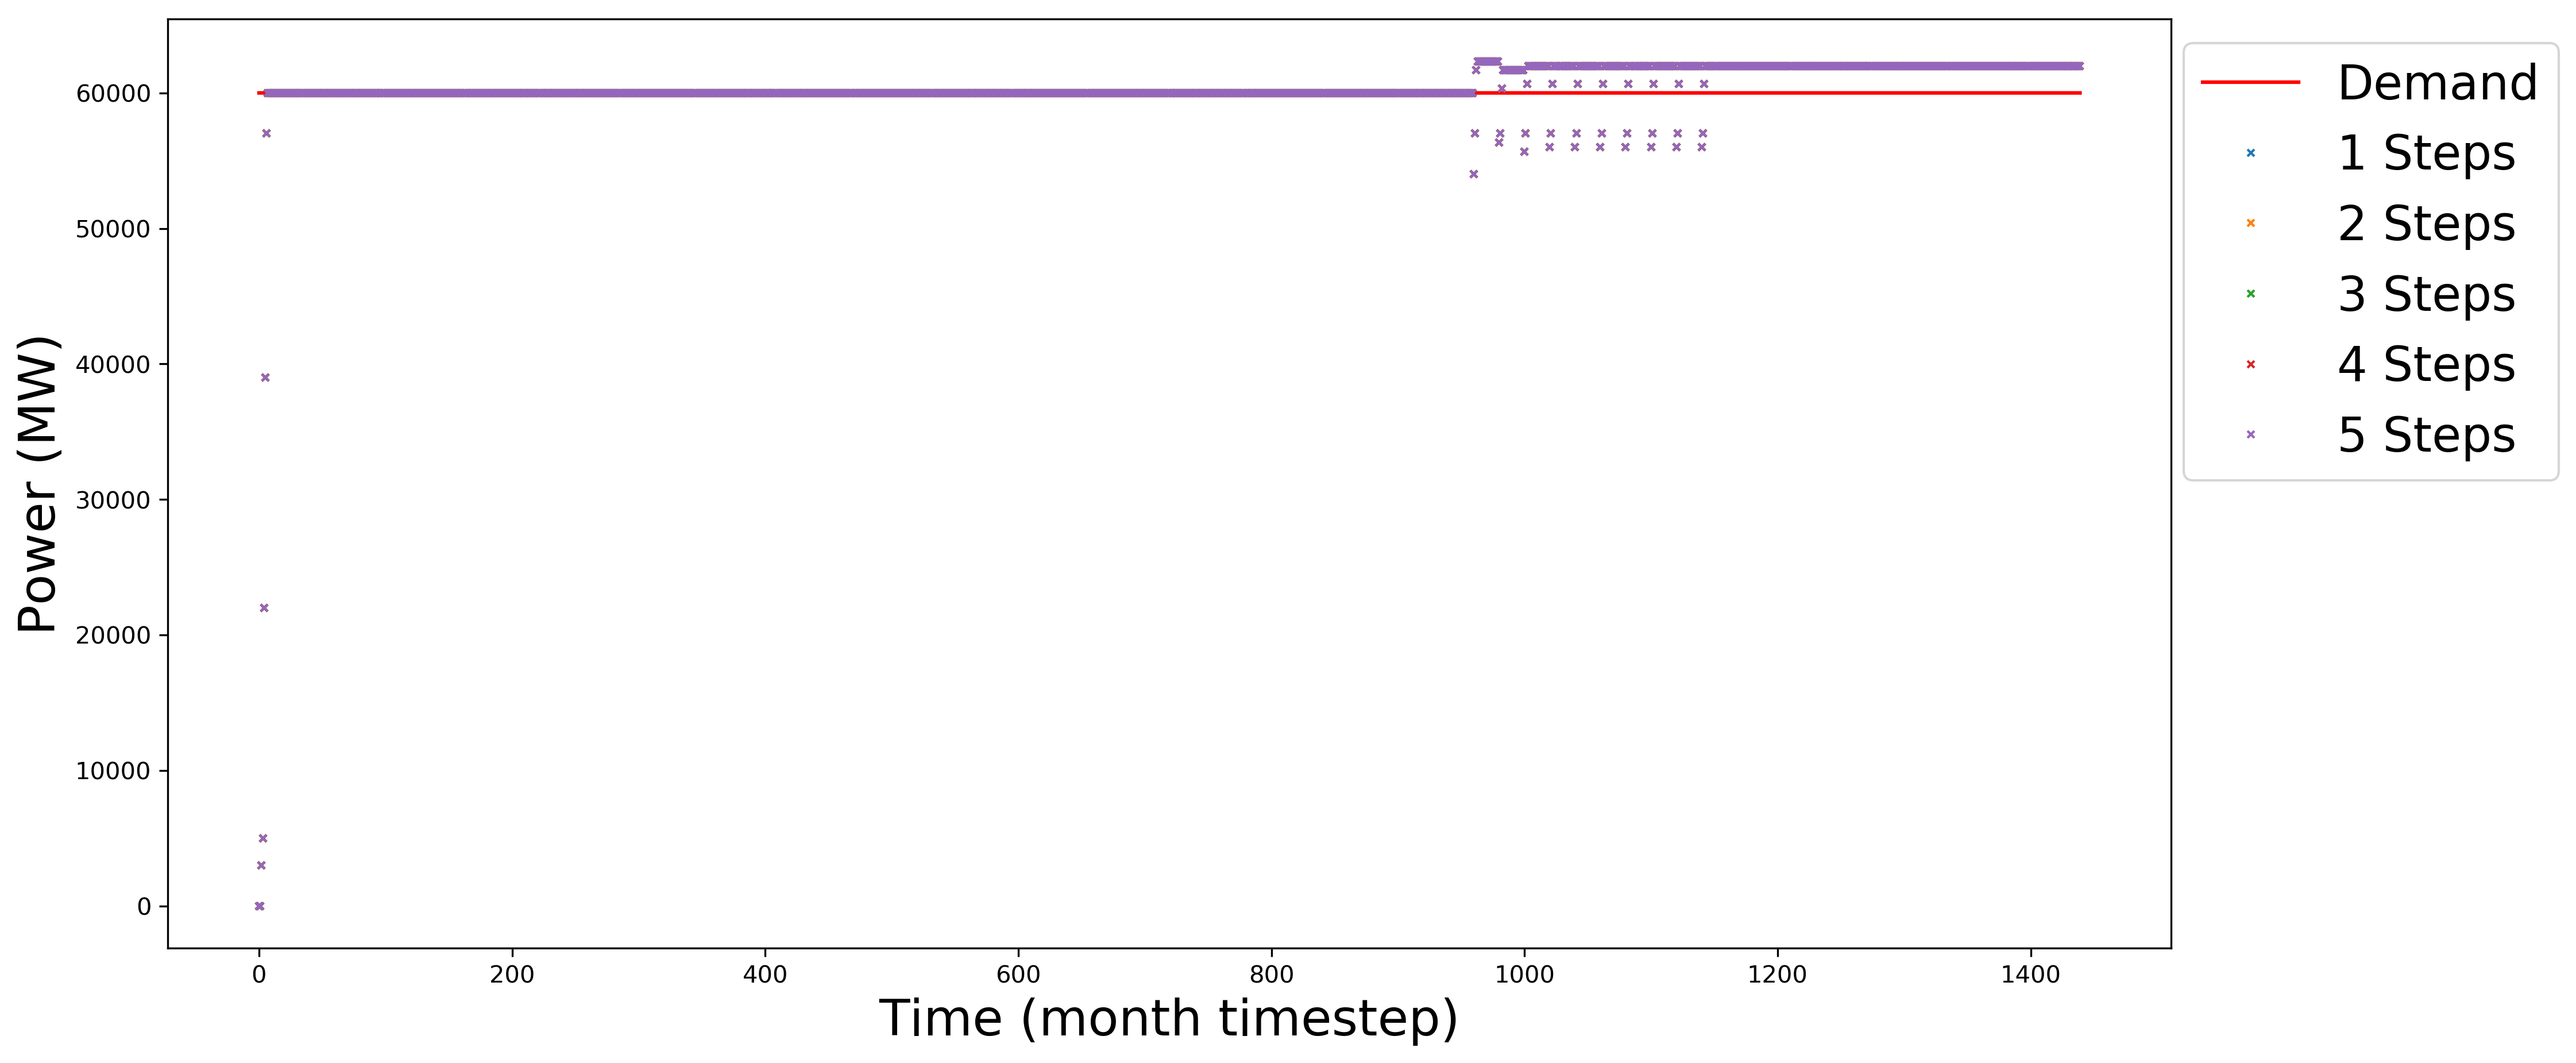
\includegraphics[width=\textwidth]{23-figures/23-power-buffer0-holt_winters-steps.png} 
	\hfill
	\caption{Power supply for different values of steps forward using holt\_winters.}
	\label{fig:23-ste-hots_winters}
\end{figure}

\begin{figure}[H]
	\centering
	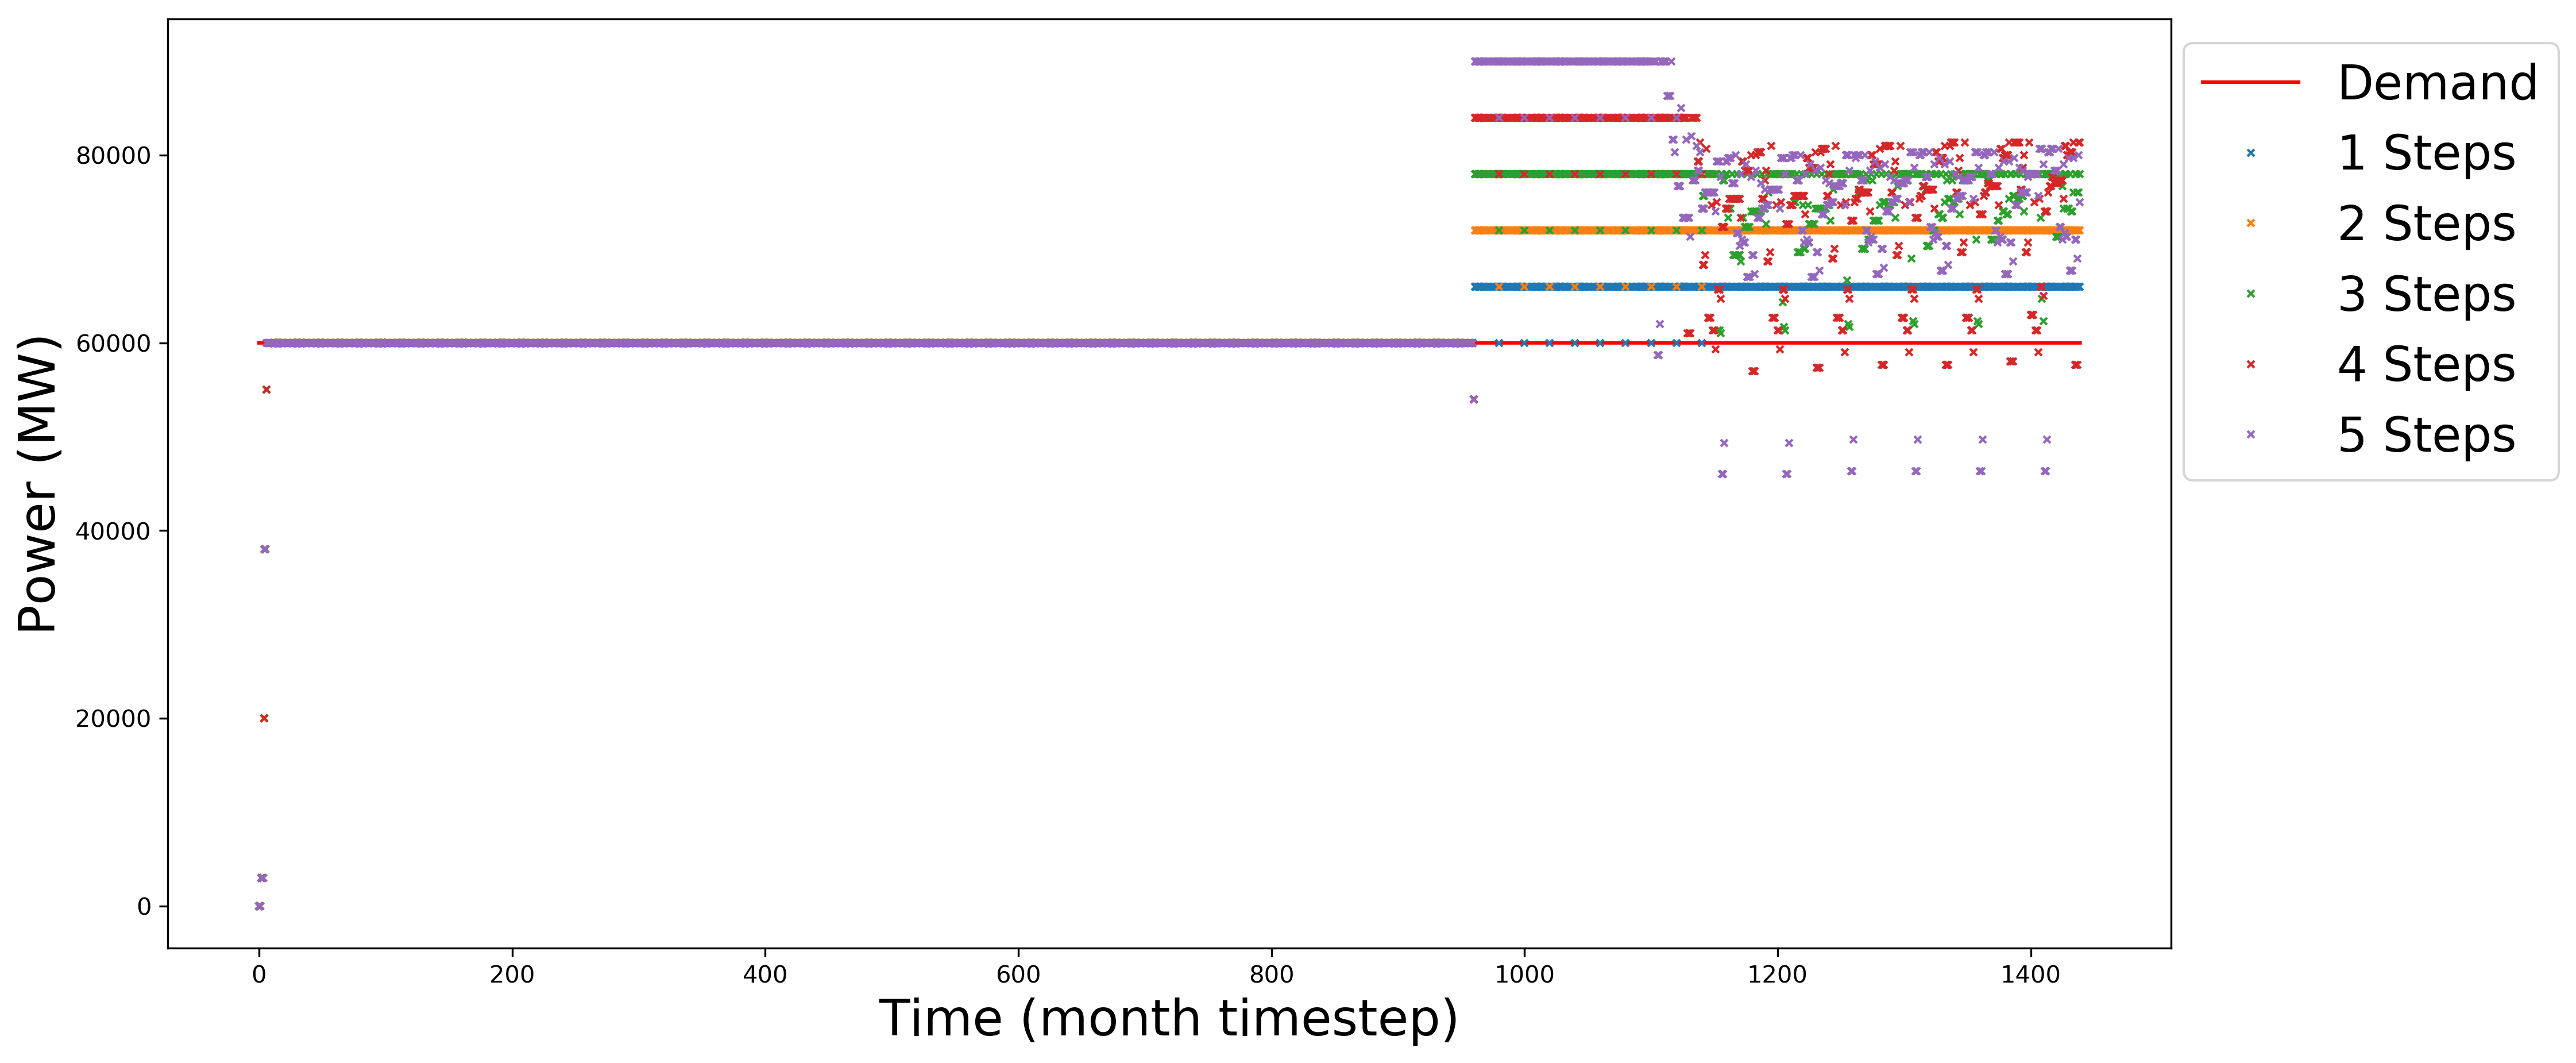
\includegraphics[width=\textwidth]{23-figures/23-power-buffer0-fft-steps.png} 
	\hfill
	\caption{Power supply for different values of steps forward using fft.}
	\label{fig:23-ste-fft}
\end{figure}

\begin{figure}[H]
	\centering
	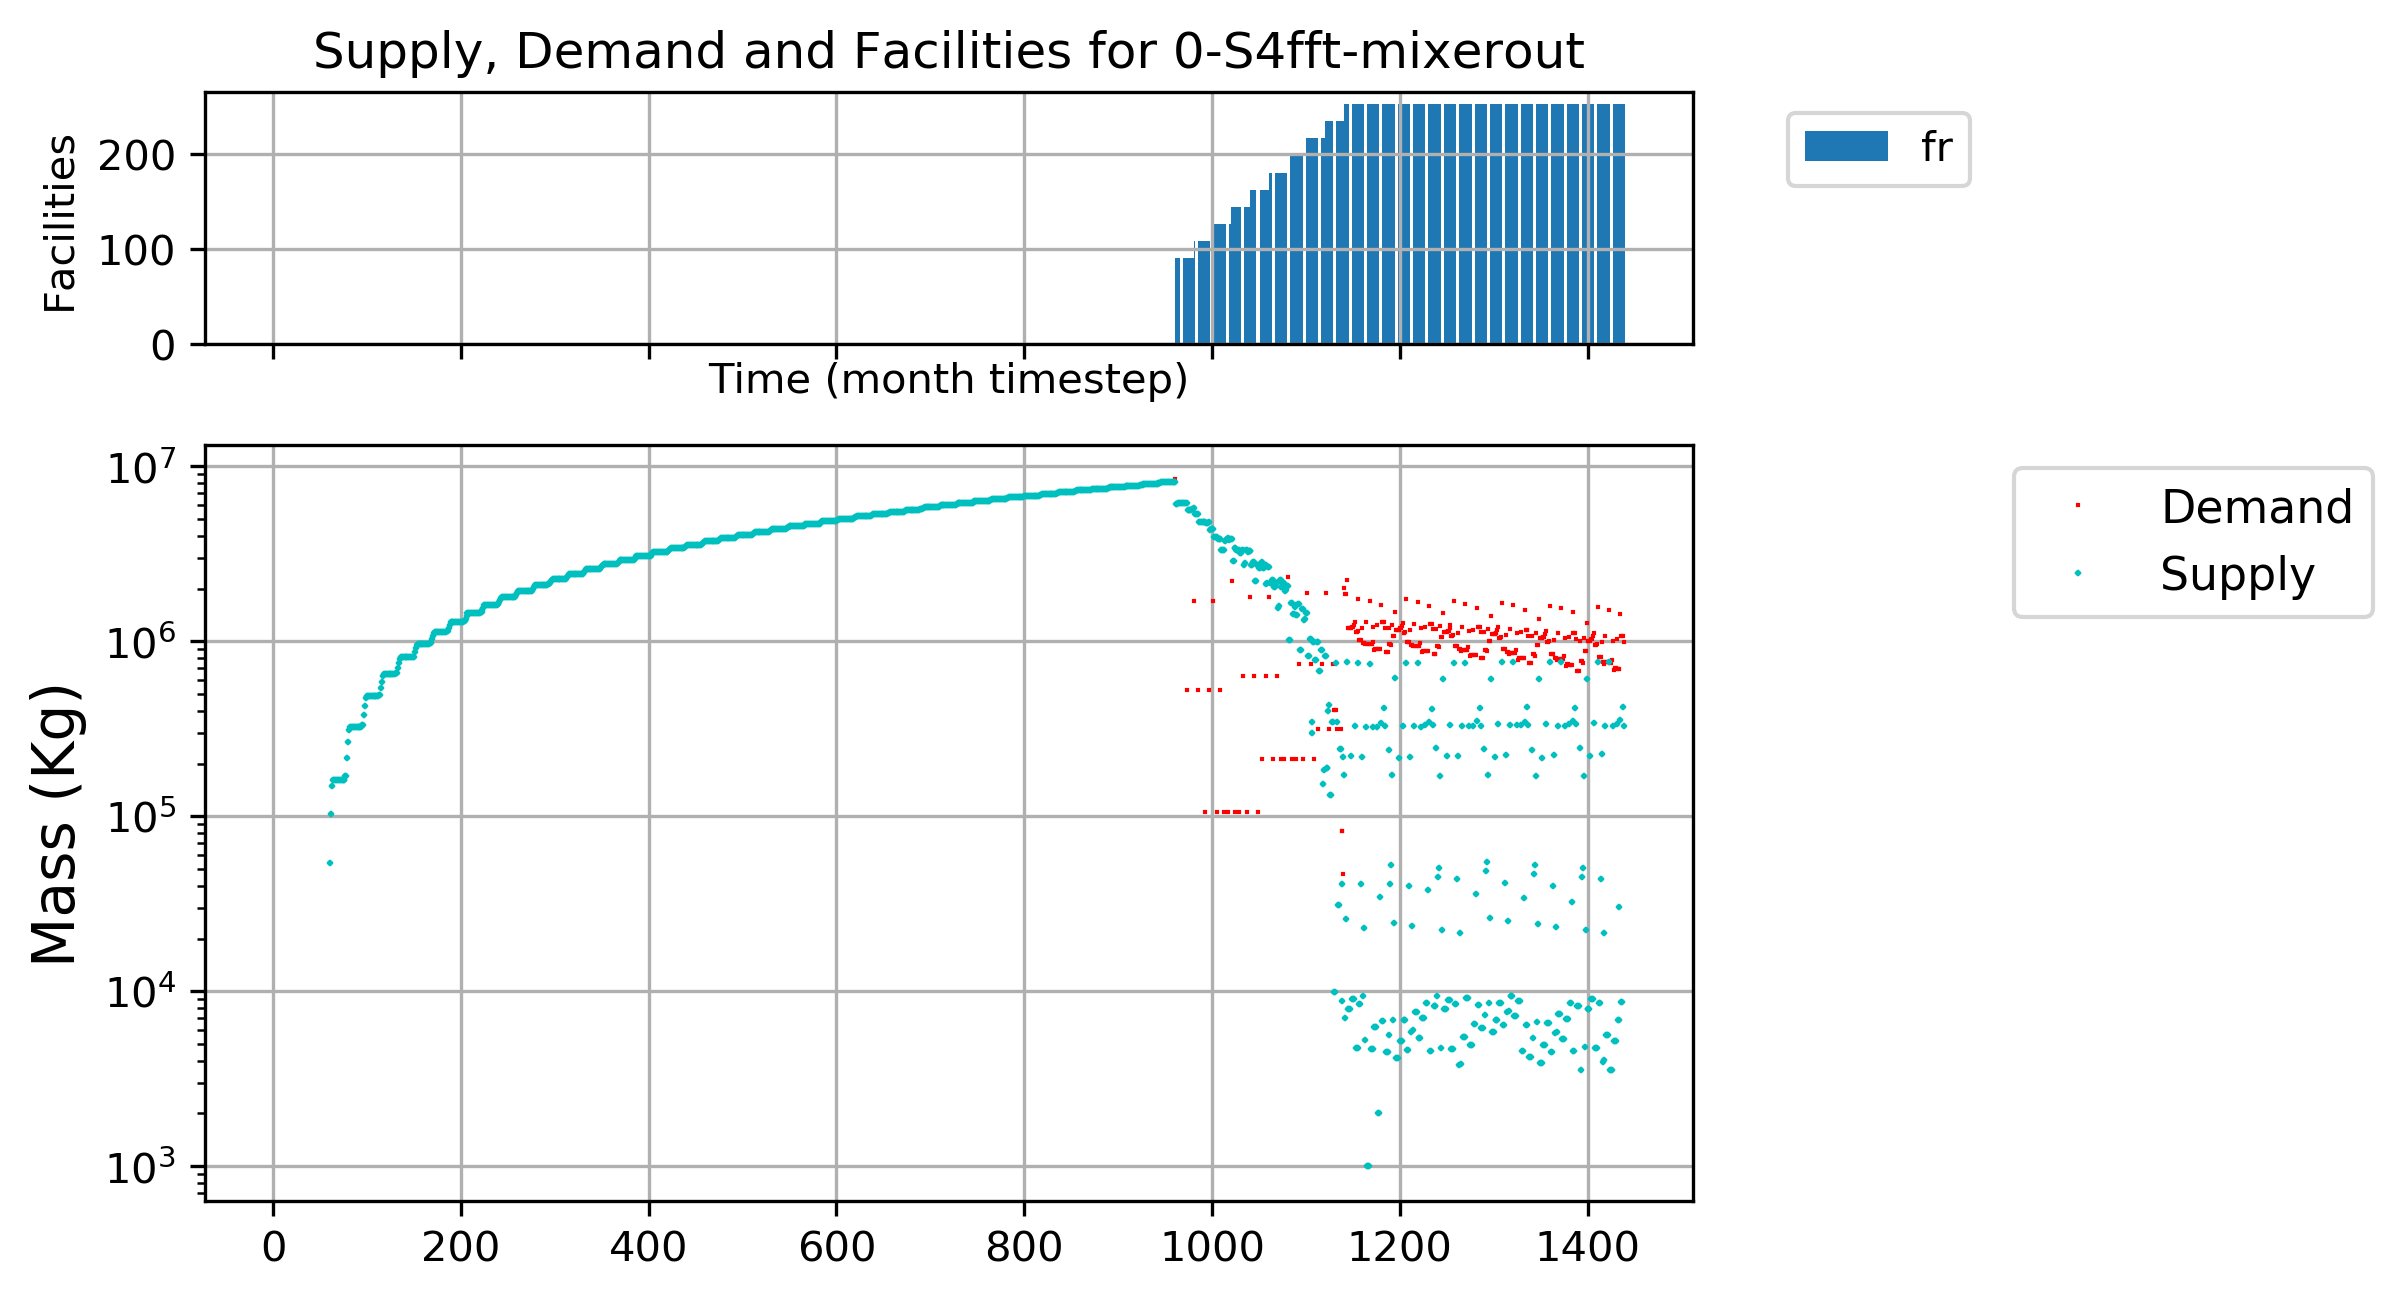
\includegraphics[width=\textwidth]{23-figures/0-S4-fft-mixerout.png} 
	\hfill
	\caption{Power supply for 4 steps forward using fft.}
	\label{fig:23-ste-fft-mixerout}
\end{figure}

\subsection{Back steps}

This section presents a sensitivity analysis for different values of  back steps. Figure \ref{fig:23-backs} shows a comparison of the cumulative under supply for different values of back steps.

Figures \ref{fig:23-back-ma} to \ref{fig:23-back-fft} display a comparison for some of the methods of the power supply for different values of back steps.

The input files use the installed capacity feature. The buffer is set to zero, steps is set to two, and back steps takes the values 1, 2, 3, 4, and 5.

\begin{figure}[H]
	\centering
	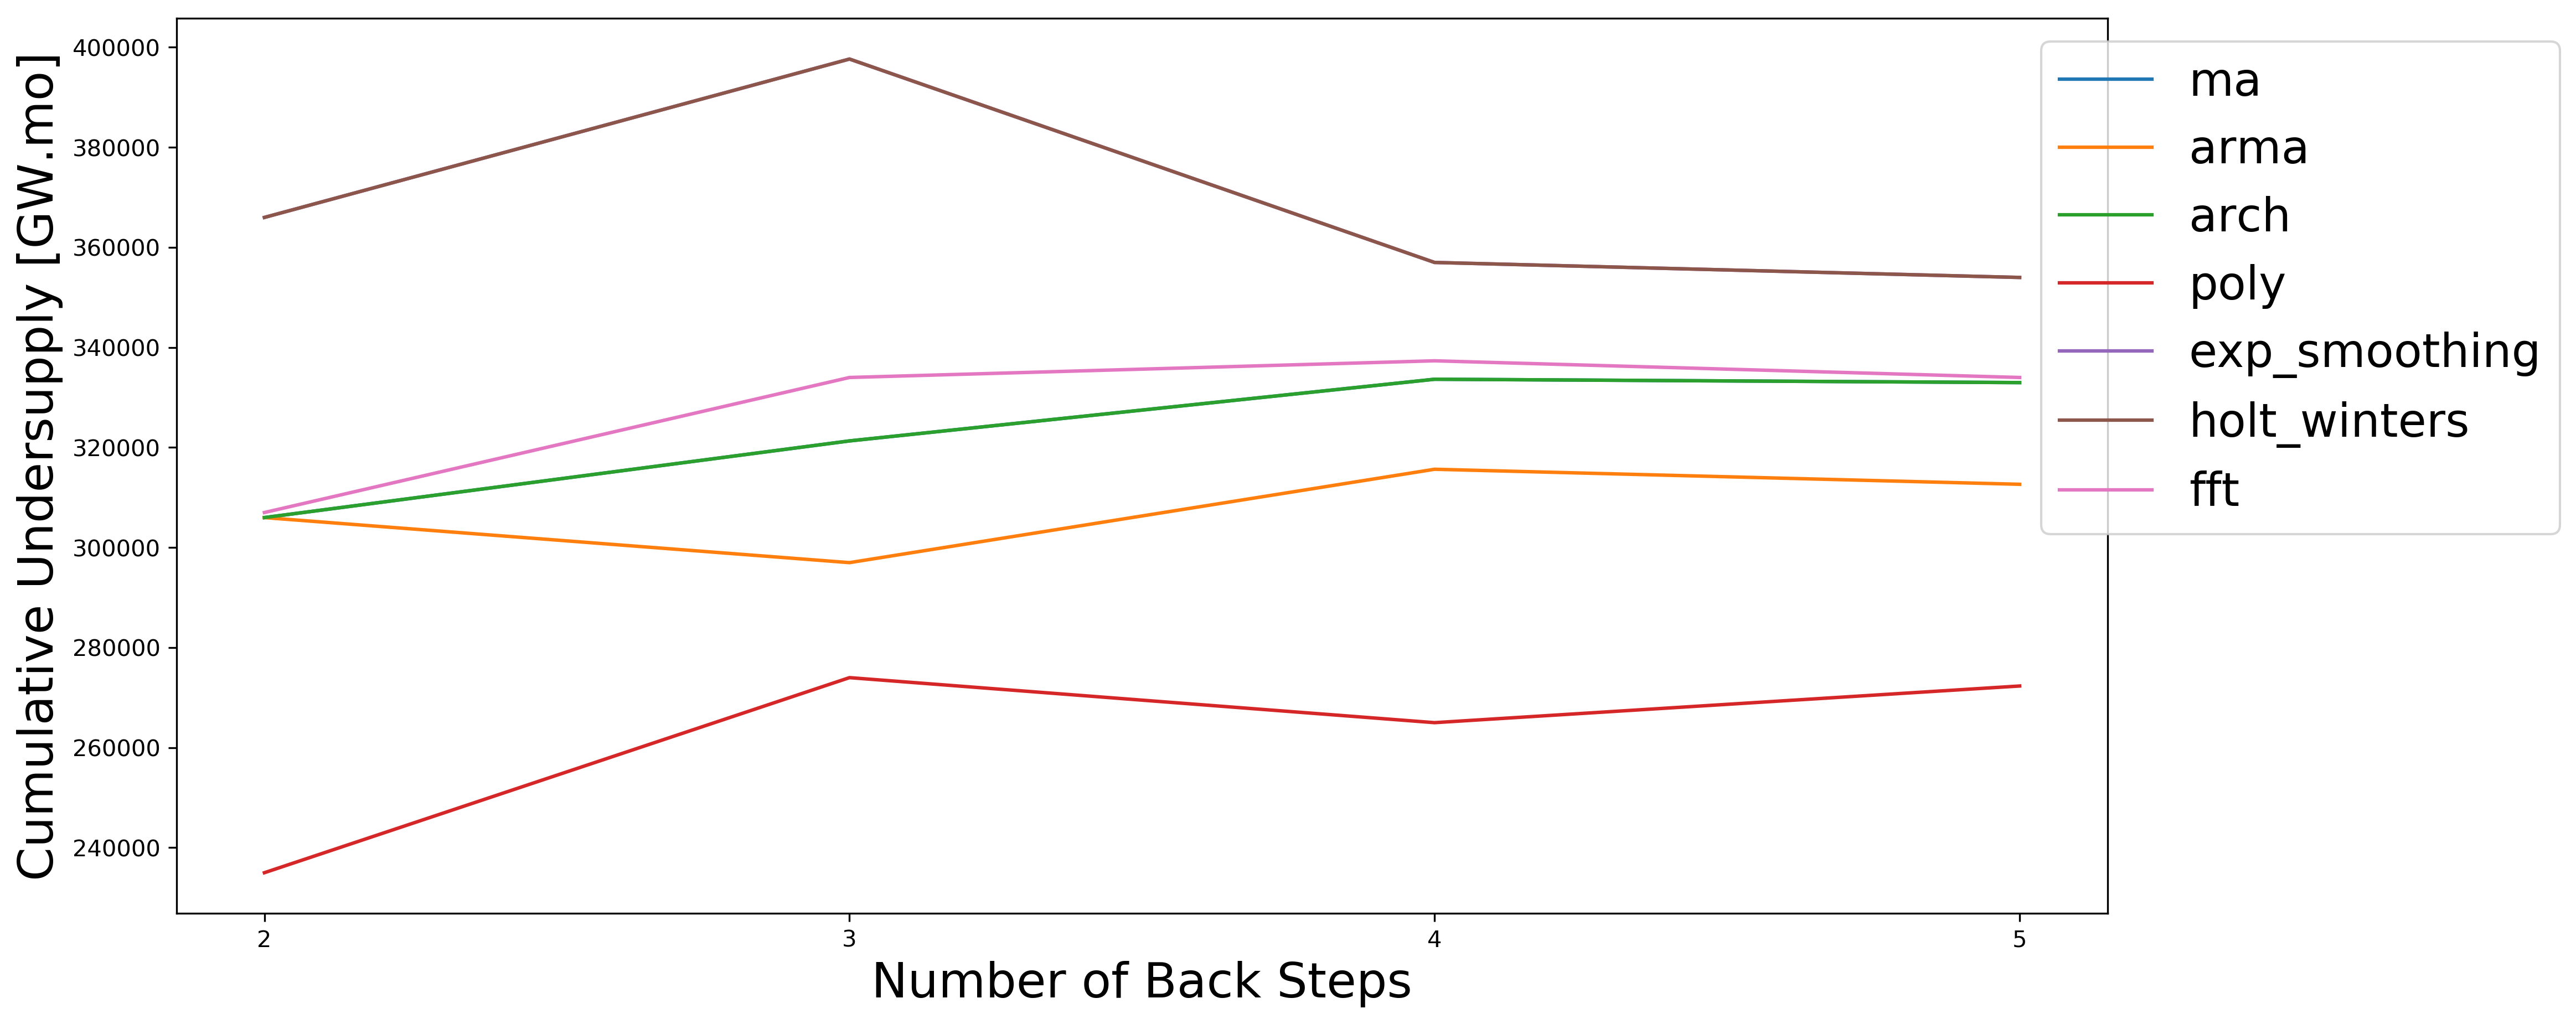
\includegraphics[width=\textwidth]{23-figures/23-sens-backs.png} 
	\hfill
	\caption{Sensitivity analysis for different number of back steps for some prediction algorithms.}
	\label{fig:23-backs}
\end{figure}

\begin{figure}[H]
	\centering
	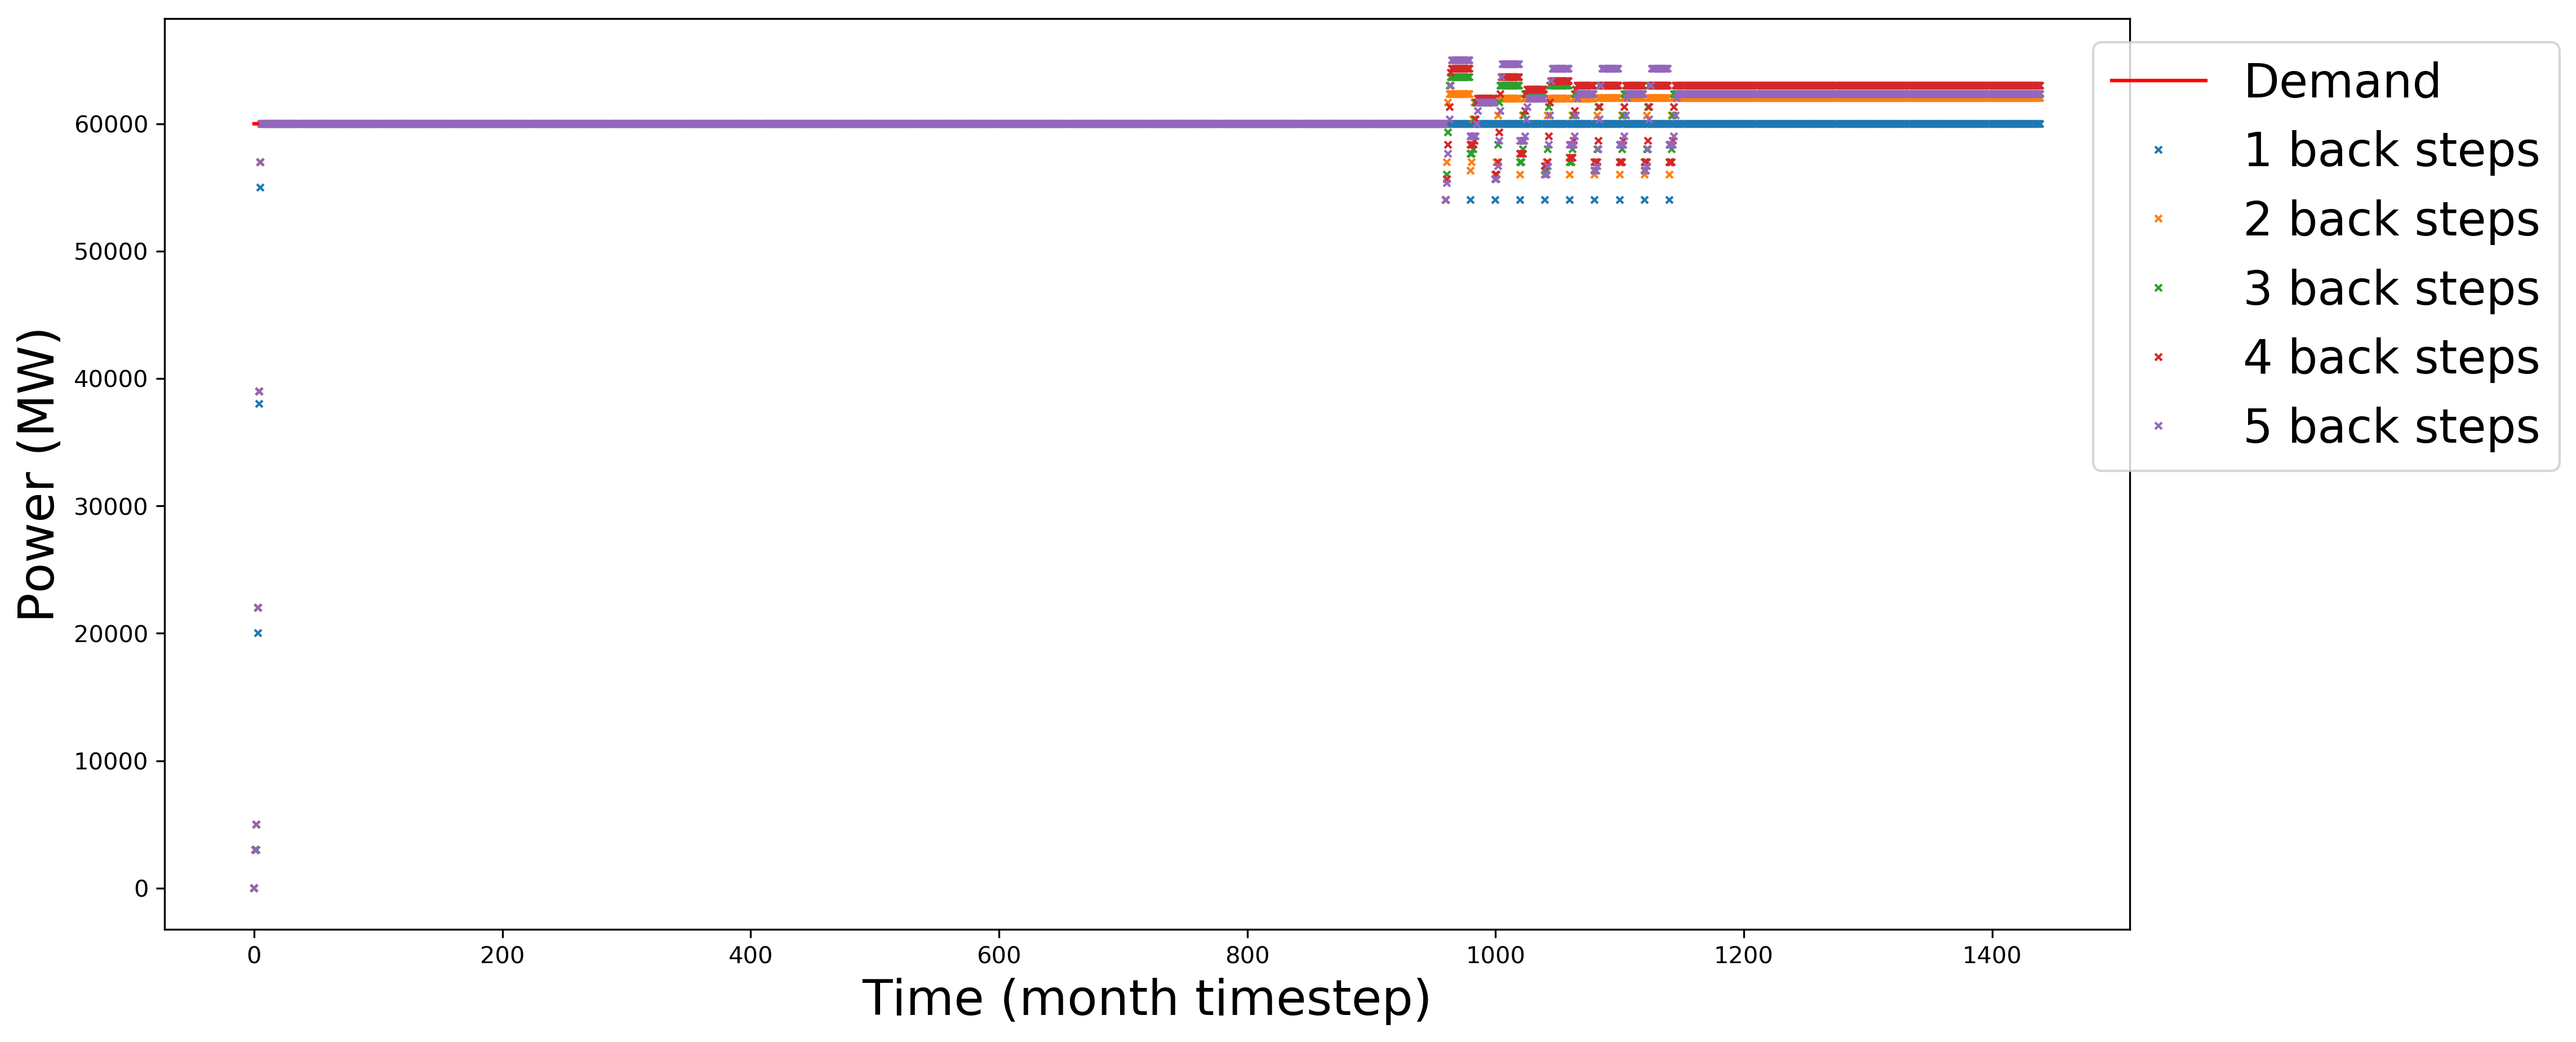
\includegraphics[width=\textwidth]{23-figures/23-power-buffer0-ma-back.png} 
	\hfill
	\caption{Power supply for different values of back steps using ma.}
	\label{fig:23-back-ma}
\end{figure}

\begin{figure}[H]
	\centering
	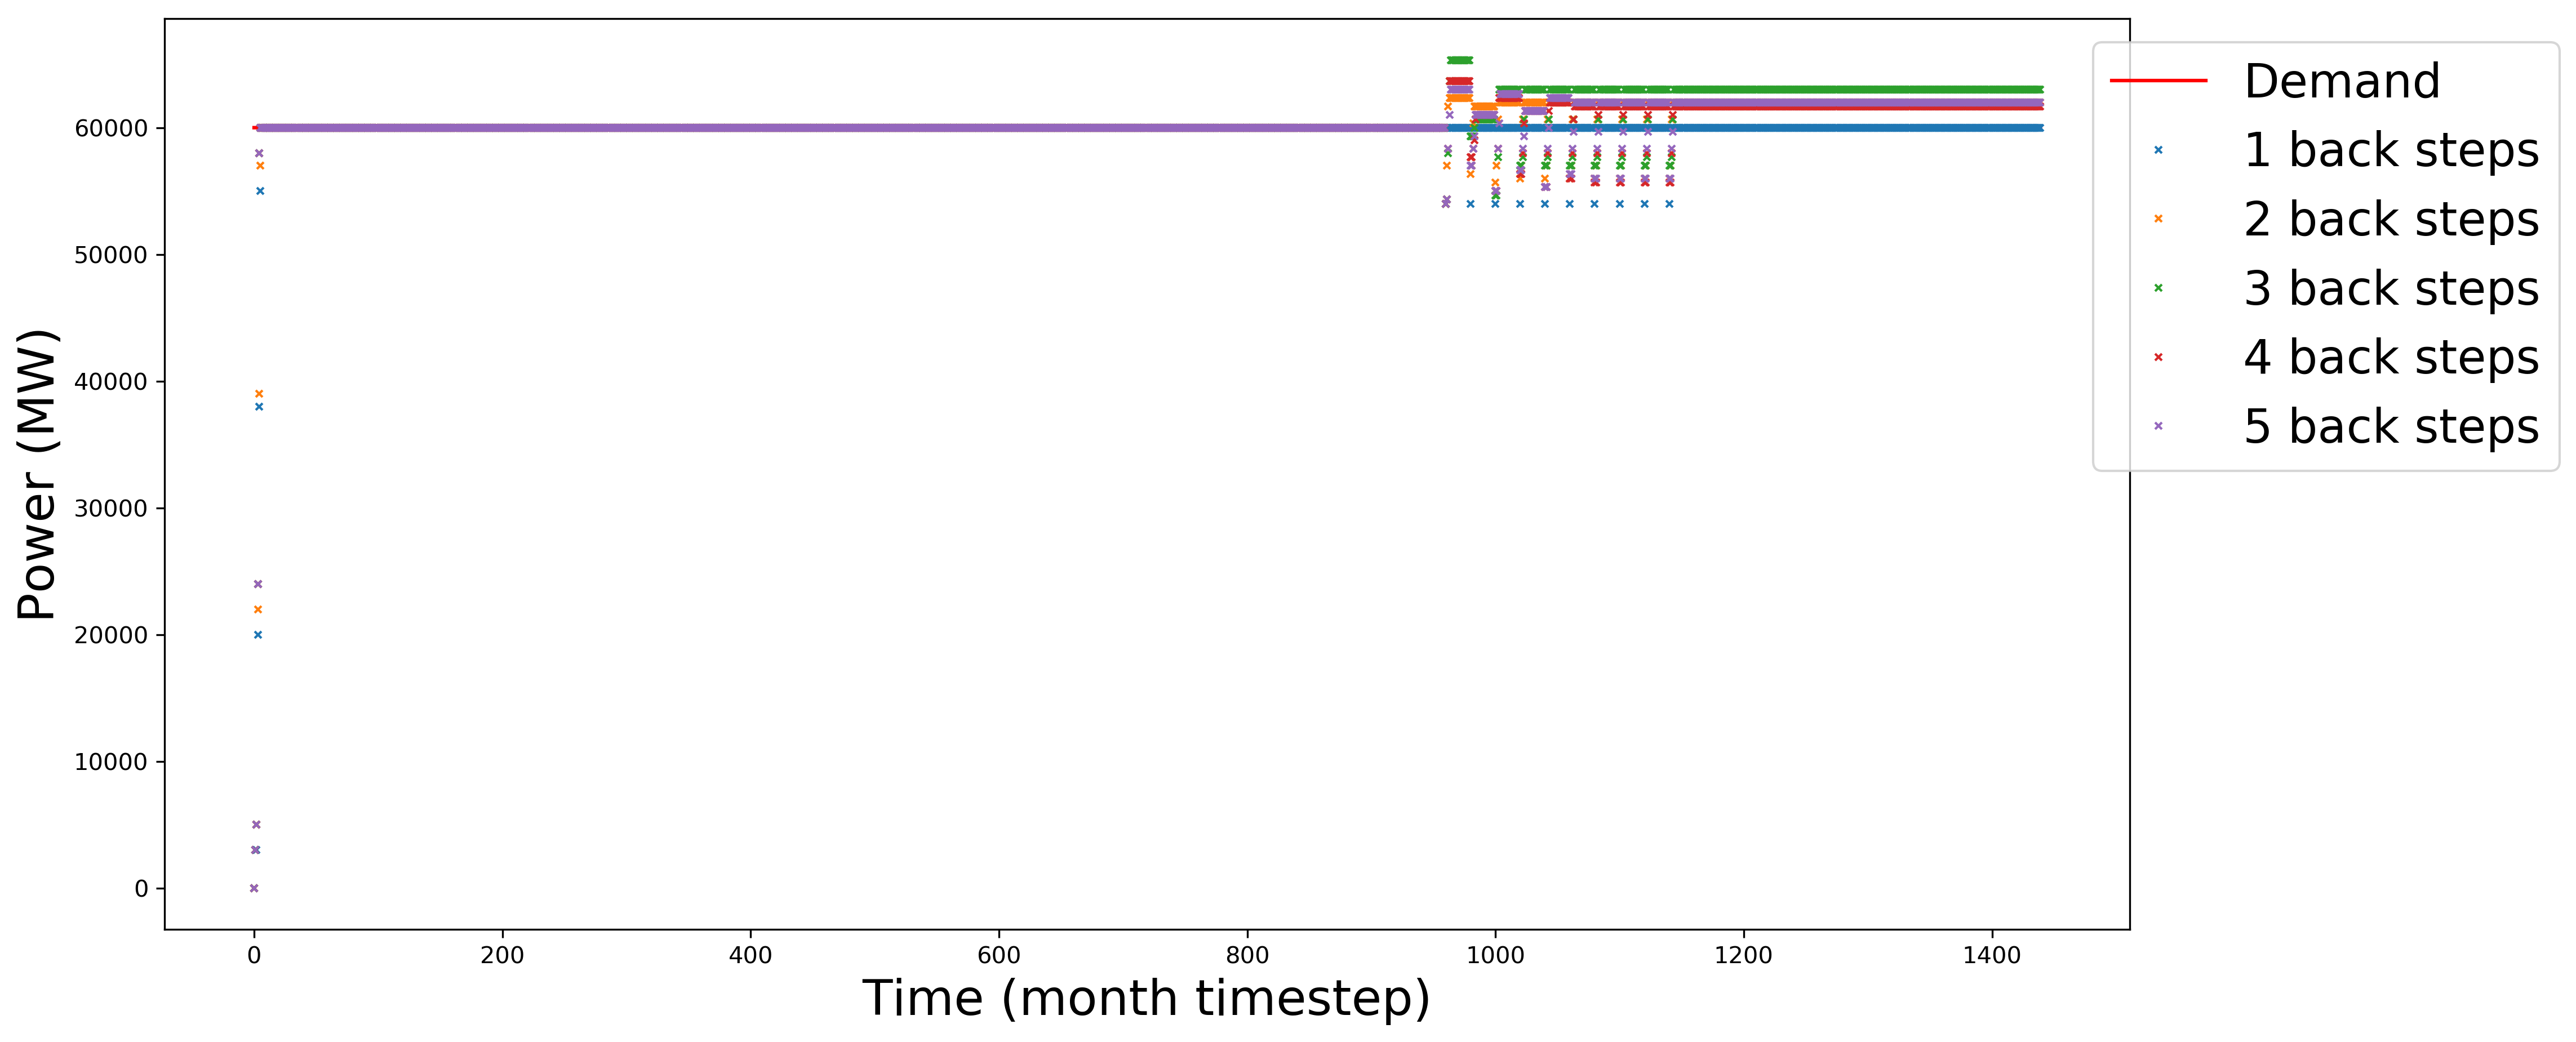
\includegraphics[width=\textwidth]{23-figures/23-power-buffer0-arma-back.png} 
	\hfill
	\caption{Power supply for different values of back steps using arma.}
	\label{fig:23-back-arma}
\end{figure}

\begin{figure}[H]
	\centering
	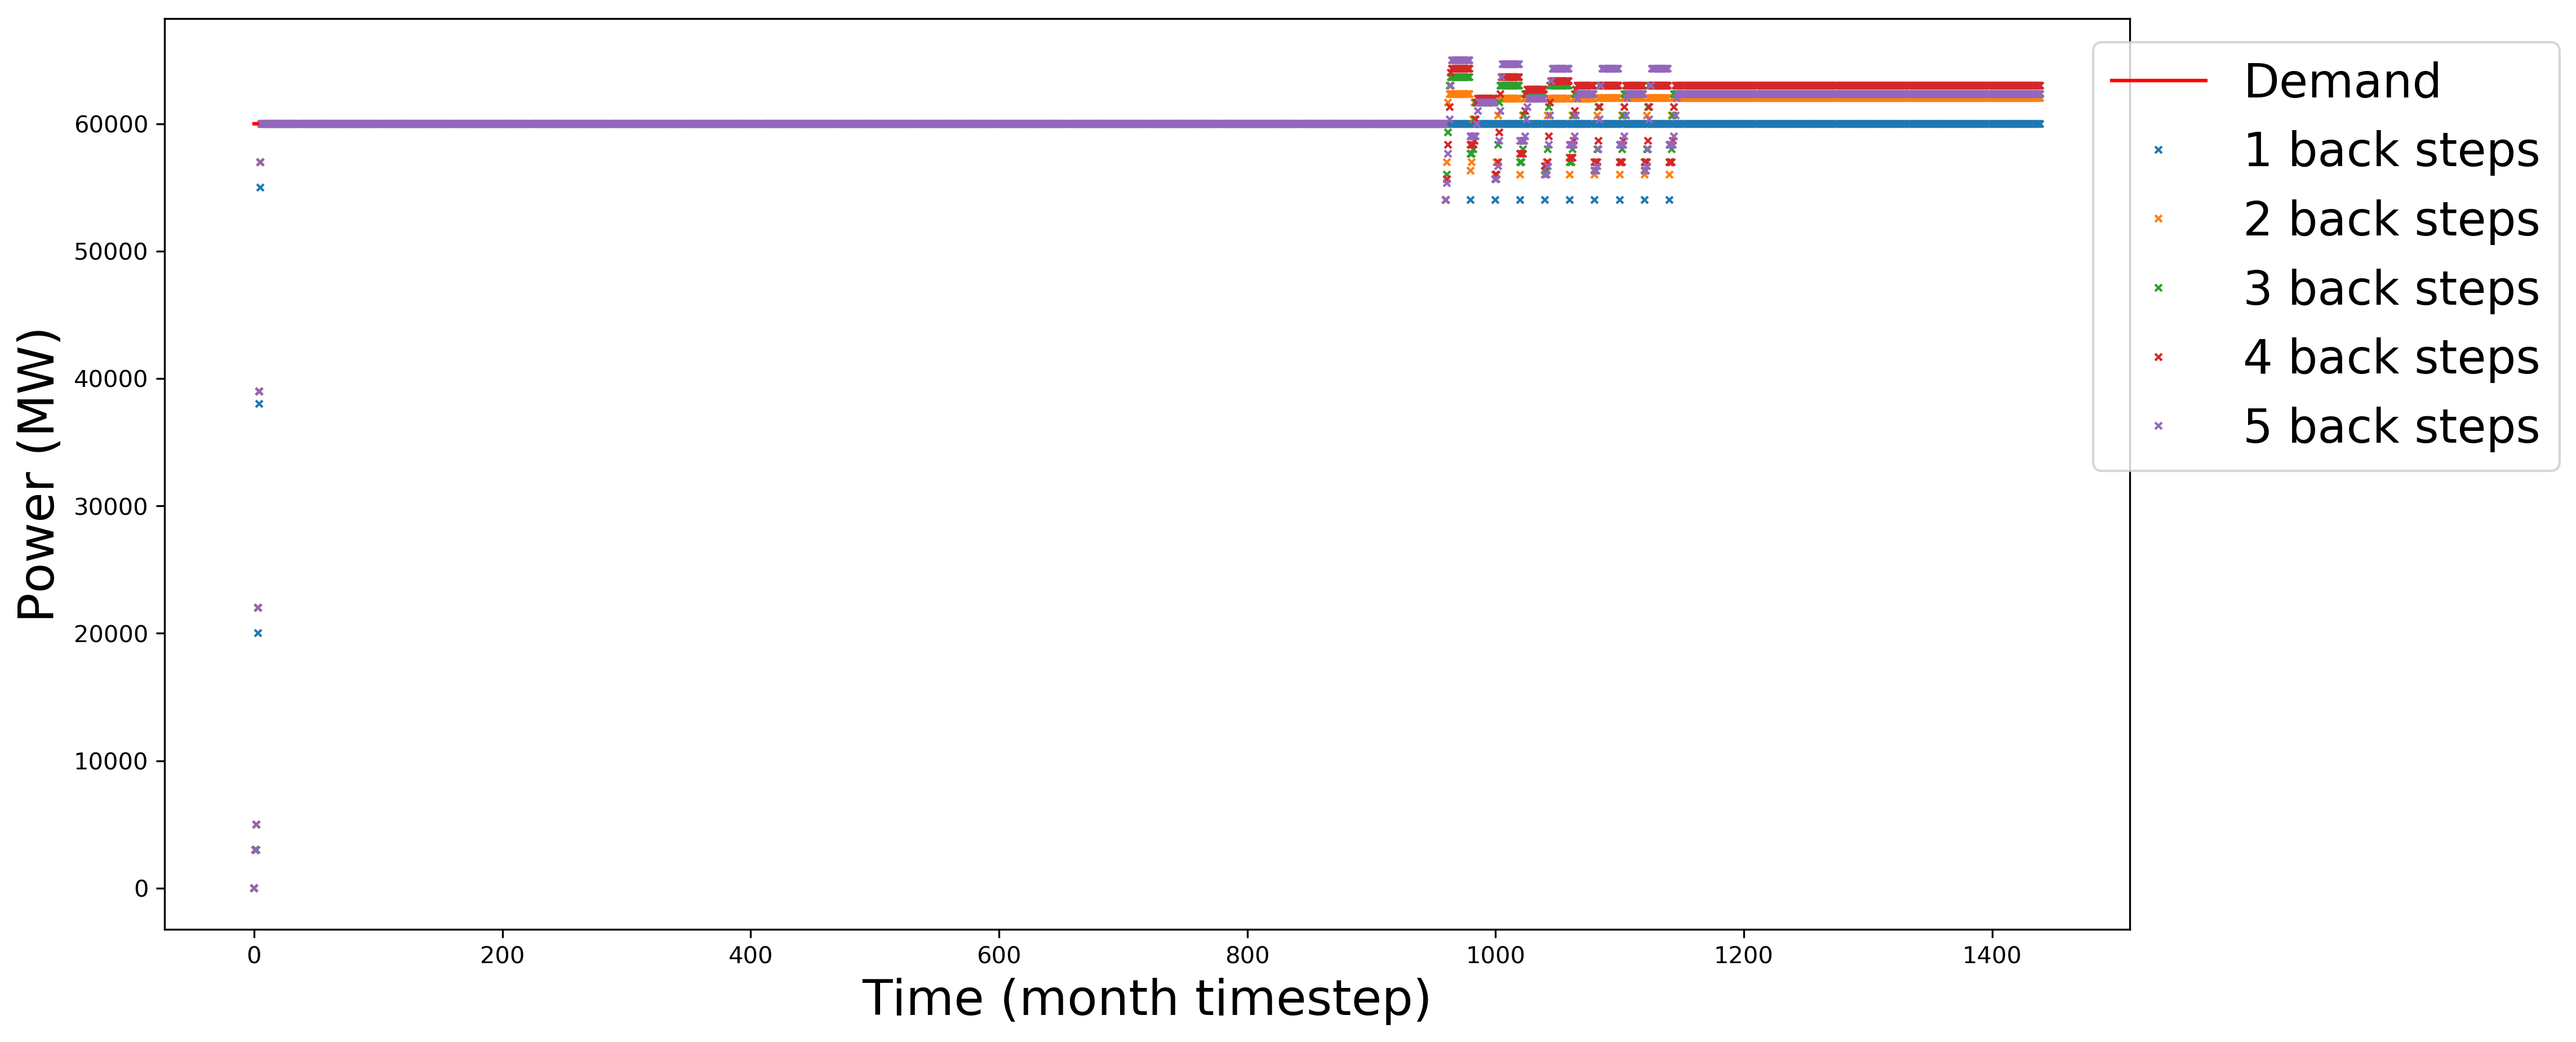
\includegraphics[width=\textwidth]{23-figures/23-power-buffer0-arch-back.png} 
	\hfill
	\caption{Power supply for different values of back steps using arch.}
	\label{fig:23-back-arch}
\end{figure}

\begin{figure}[H]
	\centering
	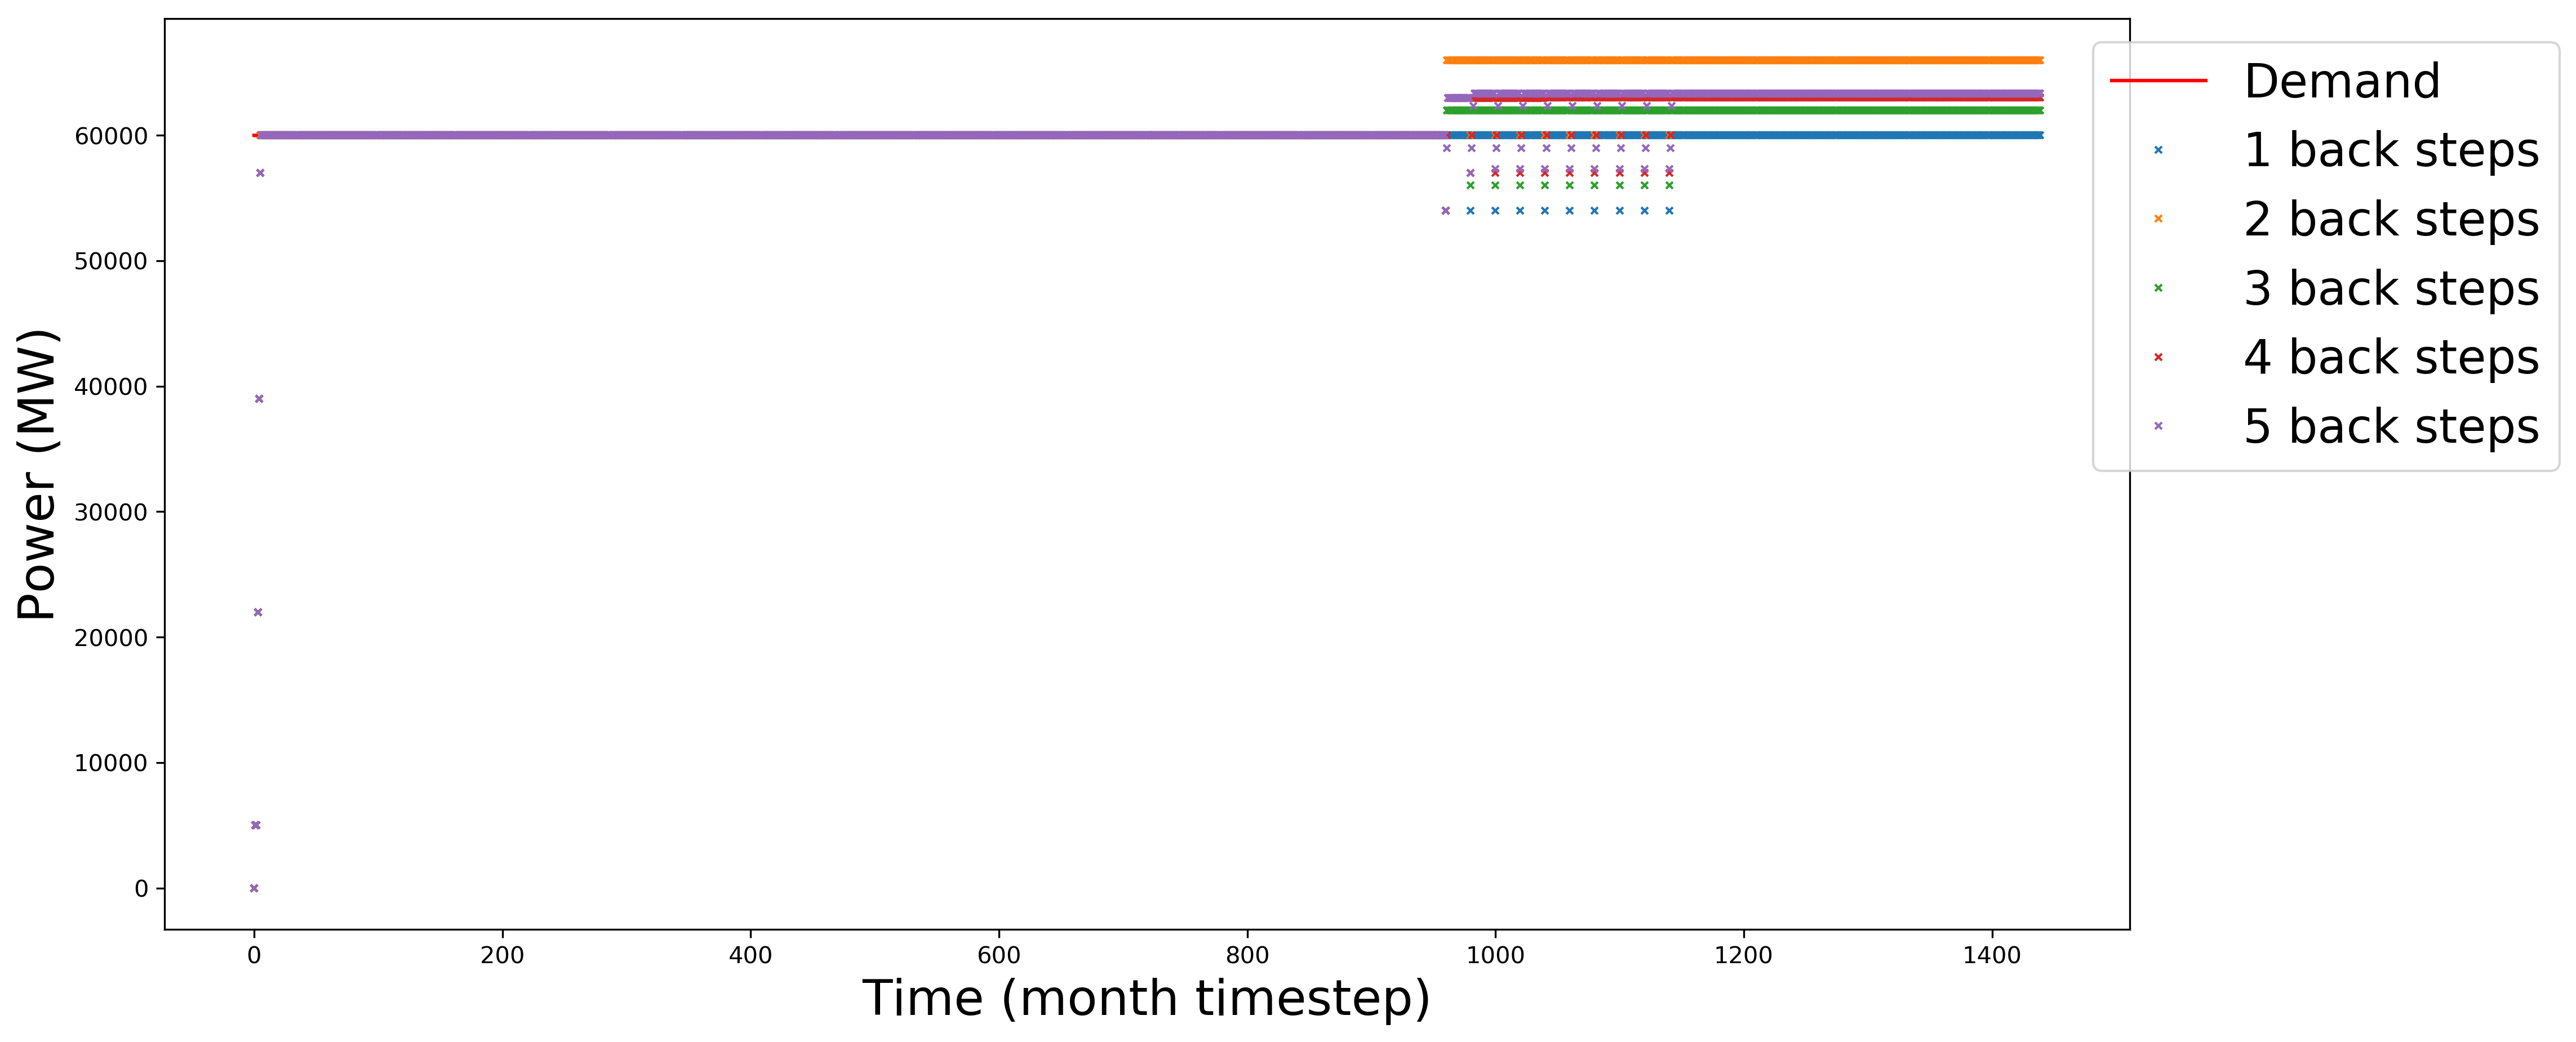
\includegraphics[width=\textwidth]{23-figures/23-power-buffer0-poly-back.png} 
	\hfill
	\caption{Power supply for different values of back steps using poly.}
	\label{fig:23-back-poly}
\end{figure}

\begin{figure}[H]
	\centering
	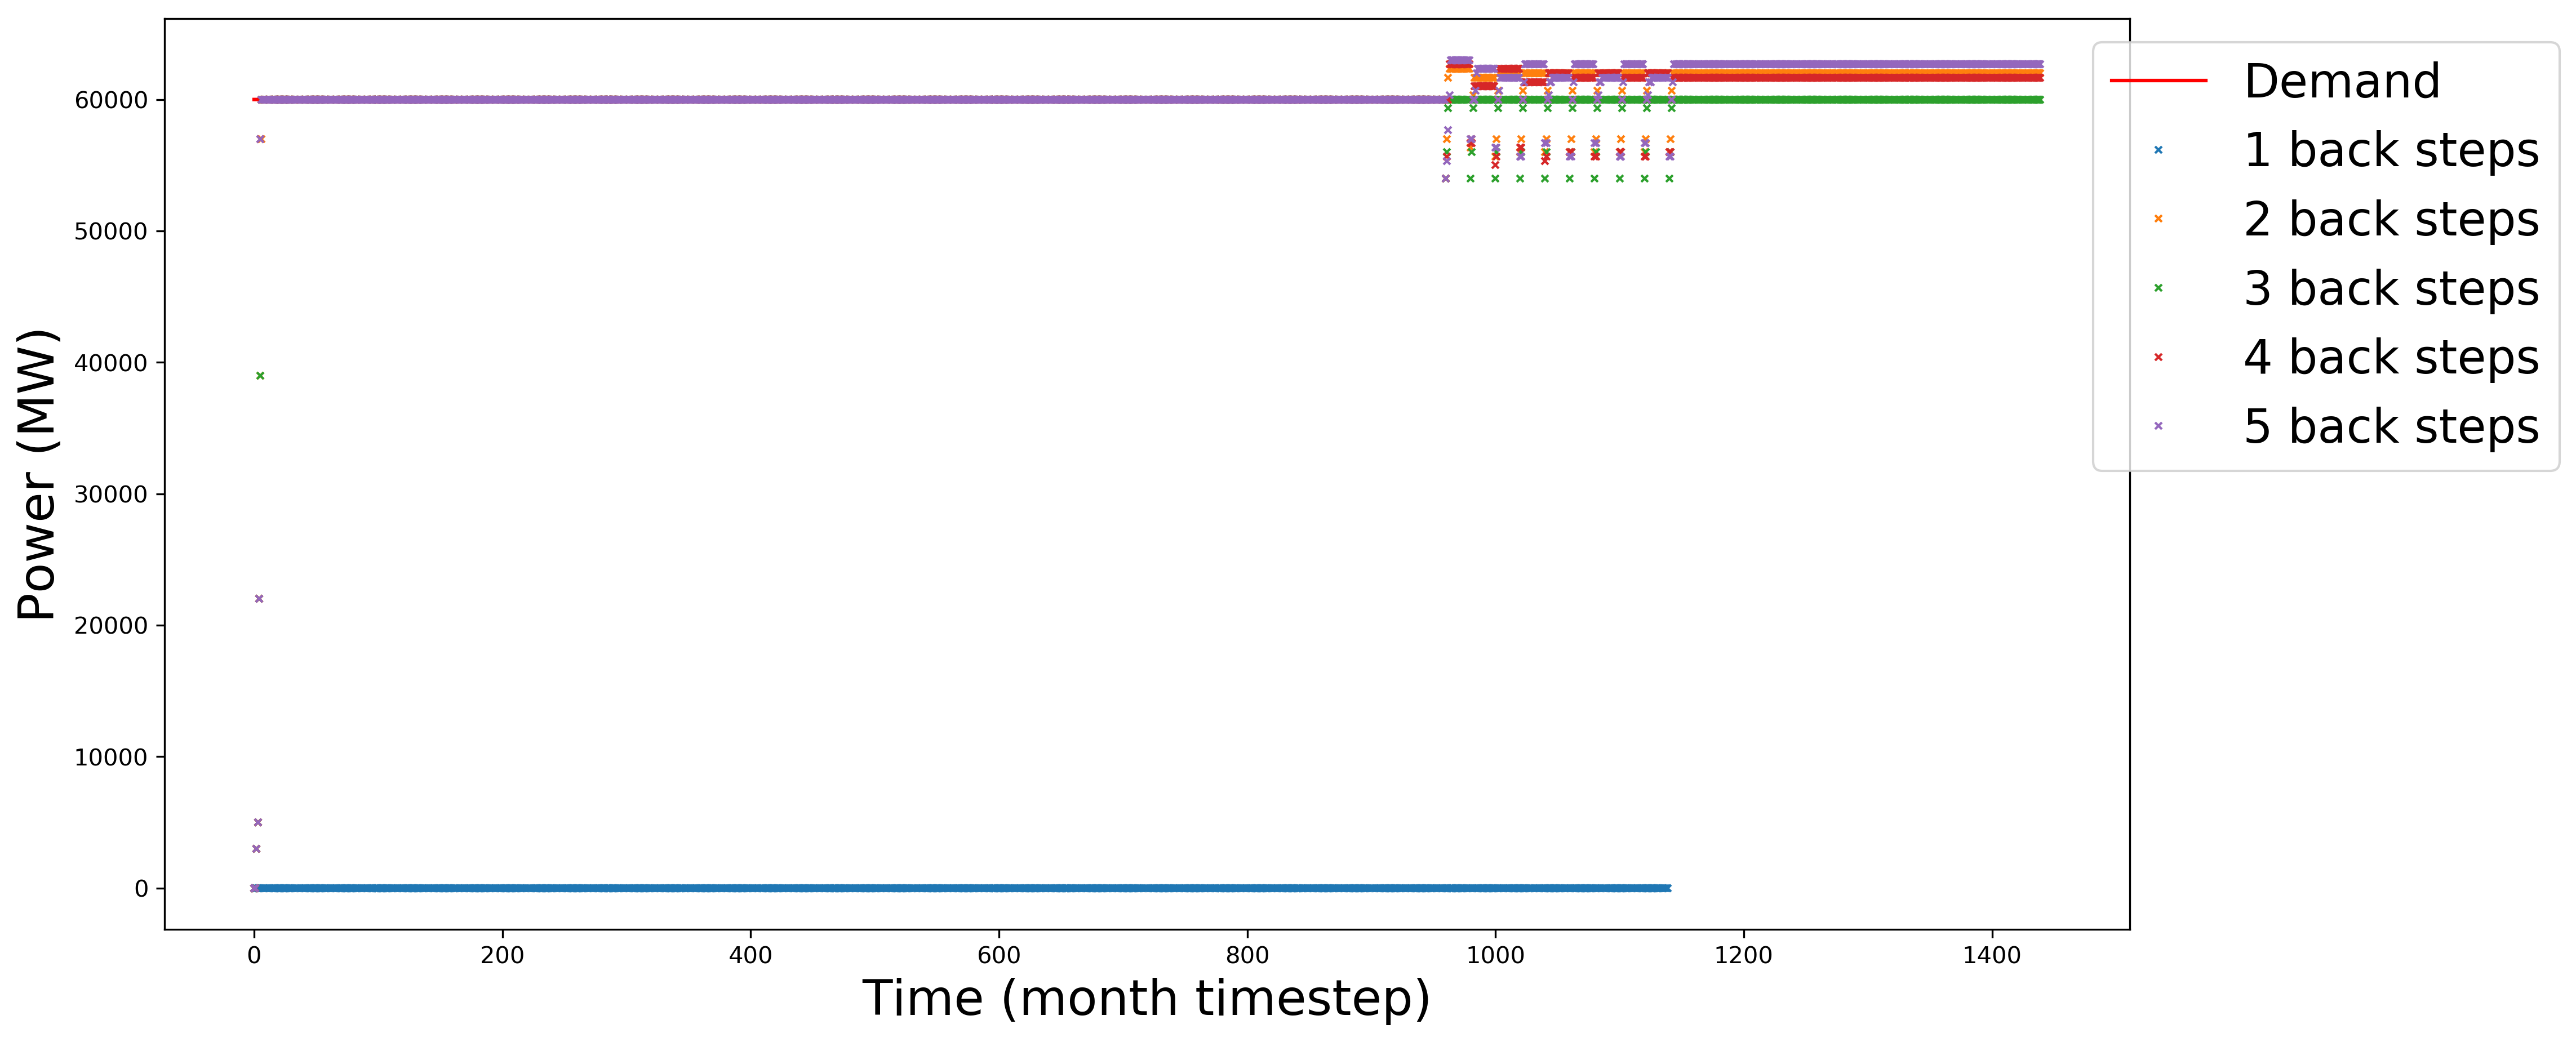
\includegraphics[width=\textwidth]{23-figures/23-power-buffer0-exp_smoothing-back.png} 
	\hfill
	\caption{Power supply for different values of back steps using exp\_smoothing.}
	\label{fig:23-back-exp_smoothing}
\end{figure}

\begin{figure}[H]
	\centering
	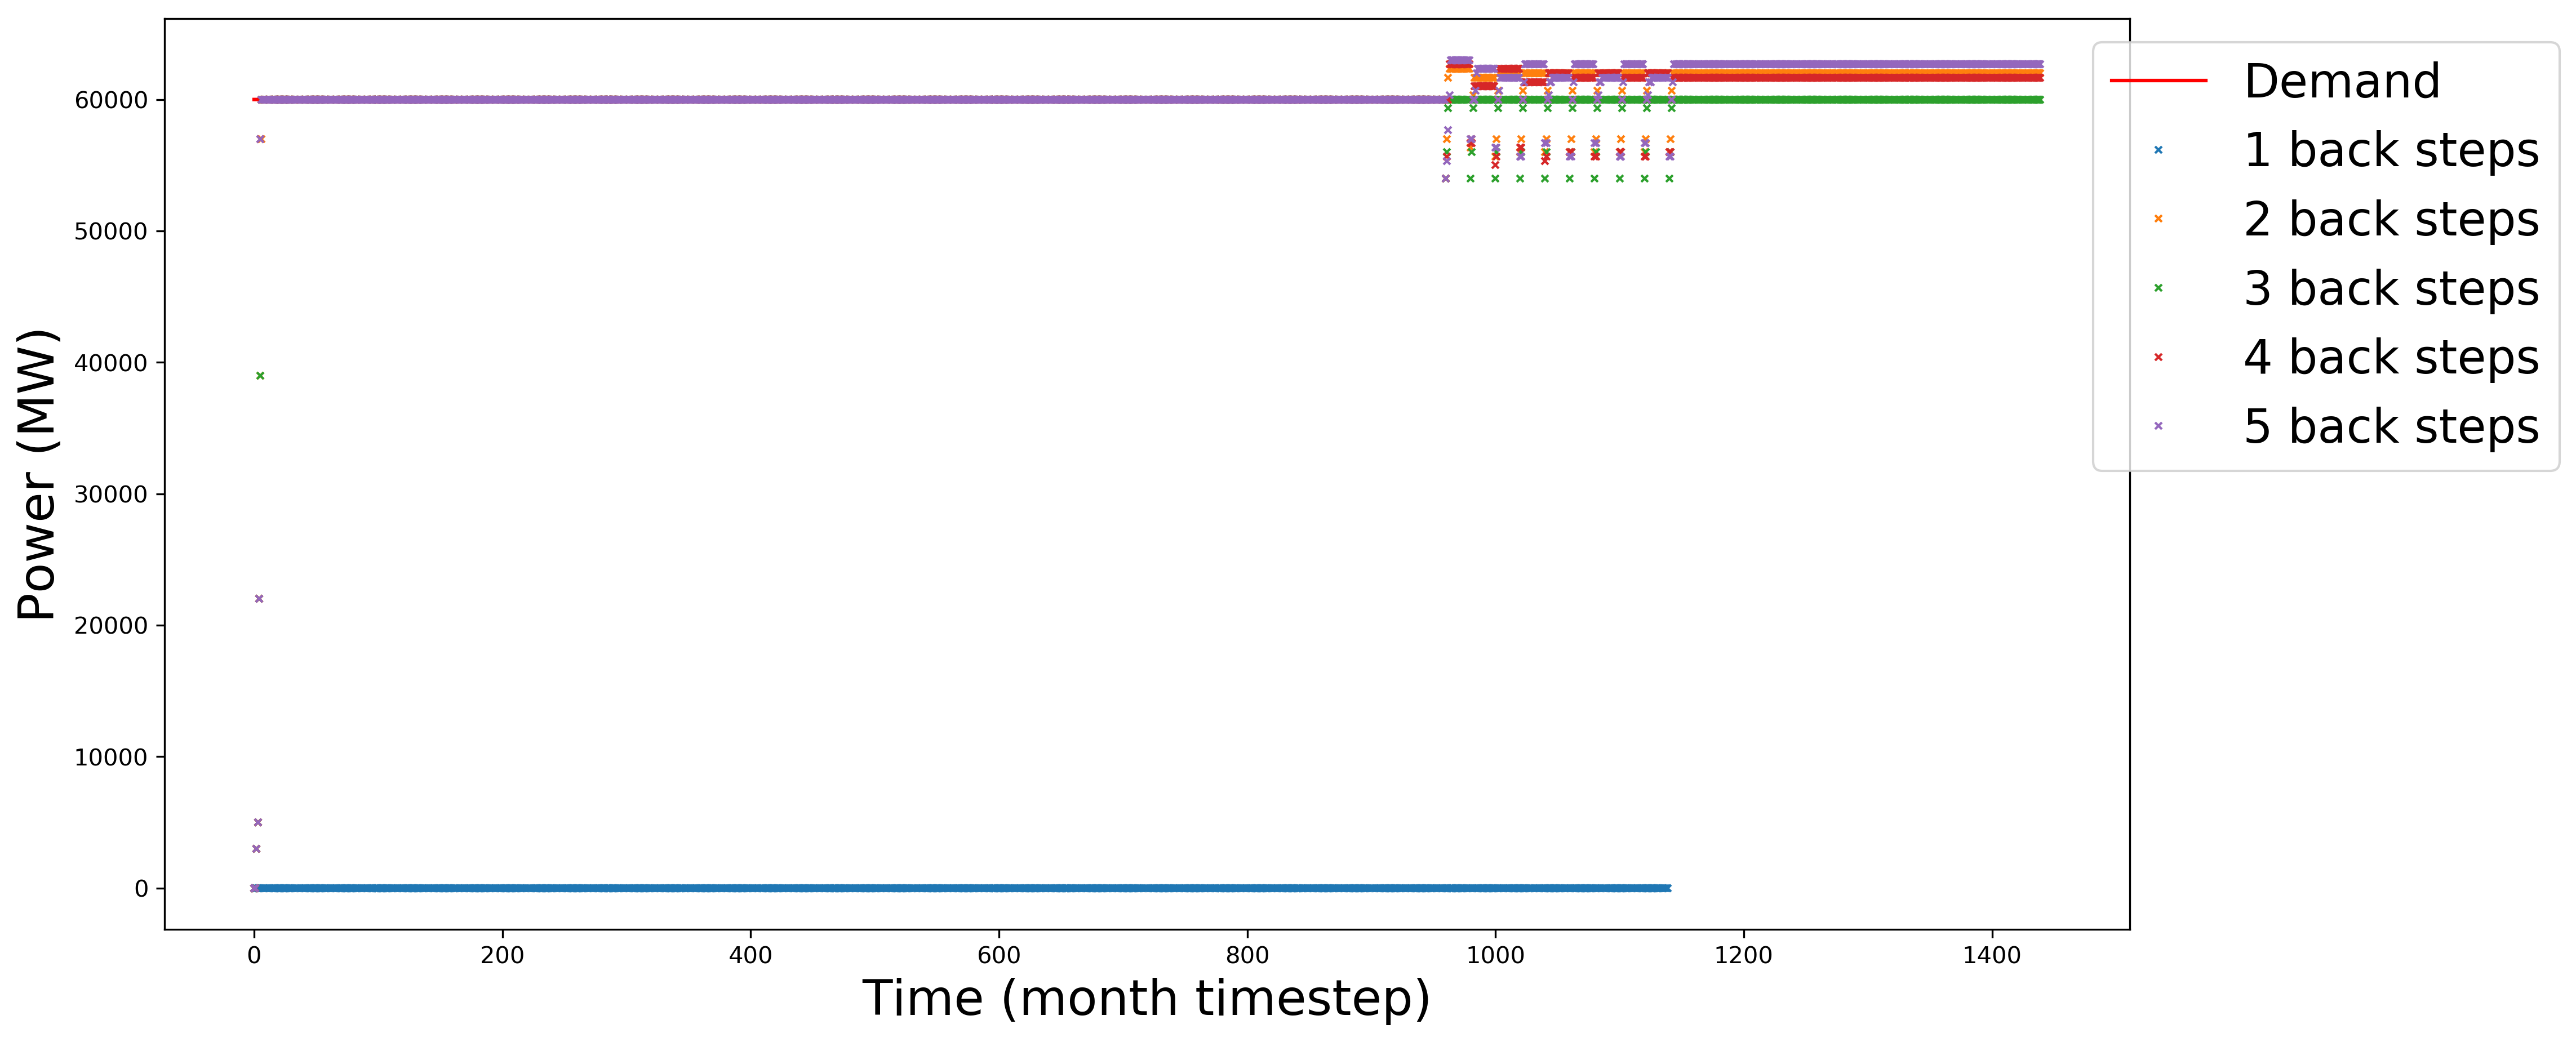
\includegraphics[width=\textwidth]{23-figures/23-power-buffer0-holt_winters-back.png} 
	\hfill
	\caption{Power supply for different values of back steps using holt\_winters.}
	\label{fig:23-back-hots_winters}
\end{figure}

\begin{figure}[H]
	\centering
	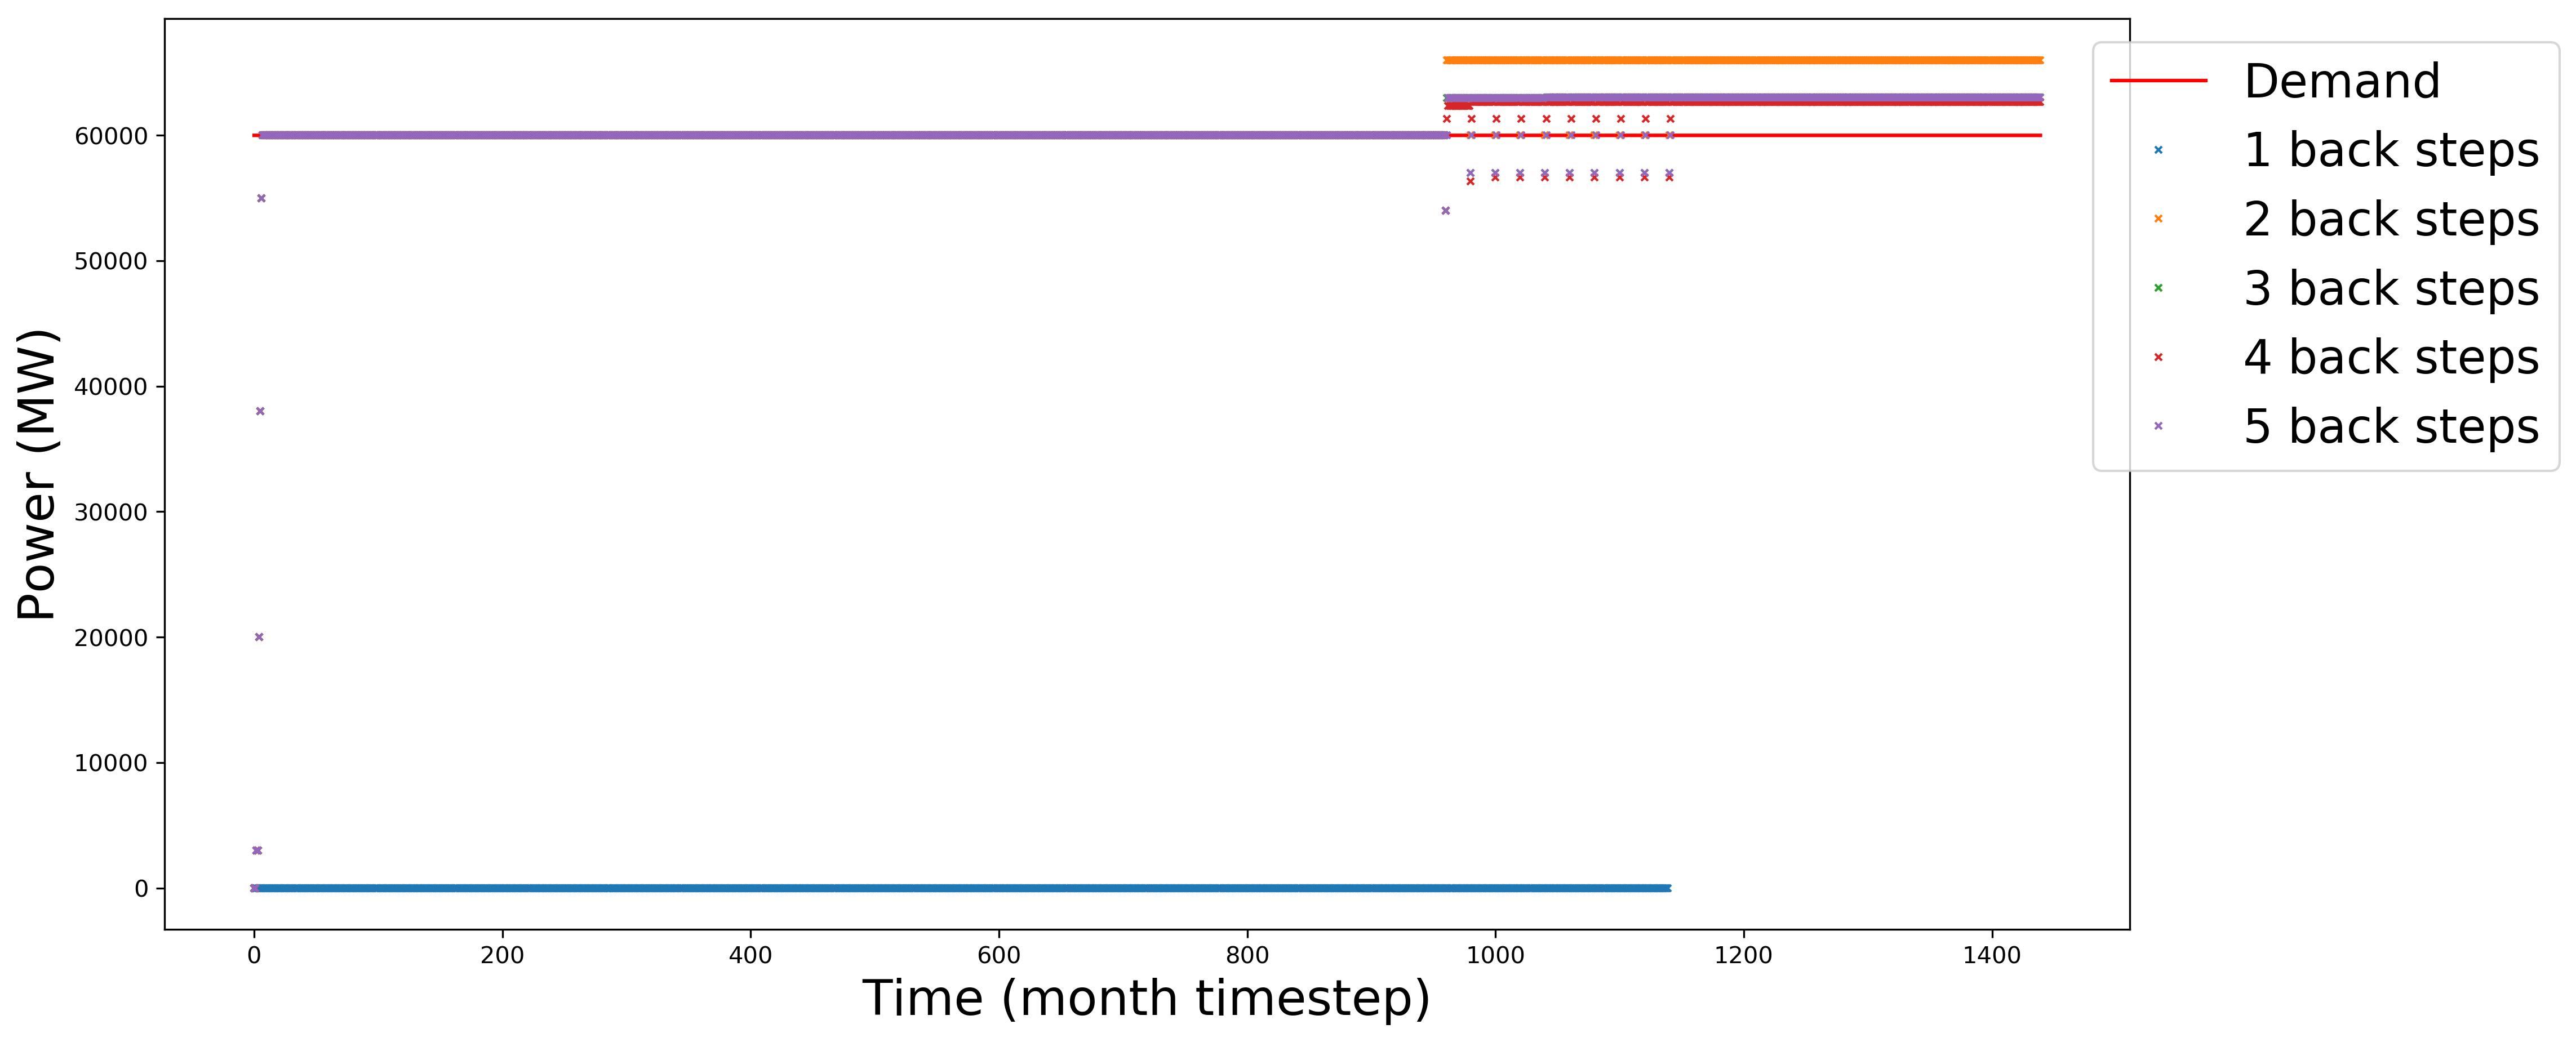
\includegraphics[width=\textwidth]{23-figures/23-power-buffer0-fft-back.png} 
	\hfill
	\caption{Power supply for different values of back steps using fft.}
	\label{fig:23-back-fft}
\end{figure}

\subsection{Different commodities}

Table \ref{tab:23-commodities} shows the name of the variables used in the simulations and what they represent in the cycle. Table \ref{tab:23-commod} presents the number of steps of under supply, cumulative under supply, and cumulative oversupply for some of the commodities.

Table \ref{tab:23-commod} needs some further explanation. The simulation differentiates between front-end and back-end commodities. In this simulation, front-end commodities are power, sourceout, and enrichmentout. All the rest of the commodities are back-end. 

For the first ones, under supply means that a facility requires that commodity and the supply is not enough. Over supply, means the opposite. A facility requires that commodity but there is too much of it. In other words, the facilities that provide such commodity are over sized. D3ploy can avoid this situation by deploying more facilities with smaller sizes.

For the back-end commodities, the notion of under supply and over supply are different. This facilities are meant to have an accumulation of material, so they have to over sized. For example, a sink has to be large enough so we do not have to deploy new continuously. It could still happen that the sink gets full and there is a need to build a new one. This is measure by the under supply. When there is too much material that needs to be disposed and the current sinks cannot take that quantity, there is a time step with under supply. Consequently, d3ploy will deploy a new facility on the next time step.

\begin{table}[H]
	\centering
	\caption{Commodity names used in the simulation of EG01-EG23.}
	\label{tab:23-commodities}
	\begin{tabularx}{\textwidth}{lLL}
		\hline
		Commodity name  & Figure & Represents \\ \hline
  		power           & \ref{fig:23-power} & Power \\
		sourceout       & \ref{fig:23-sourceout} & Natural-U \\
        enrichmentout   & \ref{fig:23-enrichmentout} & Enriched-U \\
        mixerout        & \ref{fig:23-mixerout} & FR fuel \\
  		lwrout          & \ref{fig:23-lwrout} & Spent fuel of LWRs \\
  		frout           & \ref{fig:23-frout} & Spent fuel of FRs \\
  		lwrstorageout   & \ref{fig:23-lwrstorageout} & Cooled down spent fuel of LWRs \\
  		frstorageout    & \ref{fig:23-frstorageout} & Cooled down spent fuel of FRs \\	
  		lwrpu   & \ref{fig:23-lwrpu} & Pu from spent fuel of LWRs \\
  		frpu    & \ref{fig:23-frpu} & Pu from spent fuel of FRs \\
  		lwrreprocessingwaste & \ref{fig:23-lwrreprocessingwaste} & Waste from the reprocessing of spent fuel of LWRs \\
 		frreprocessingwaste & \ref{fig:23-frreprocessingwaste} & Waste from the reprocessing of spent fuel of FRs \\ \hline

	\end{tabularx}
\end{table}

\begin{figure}[H]
	\centering
	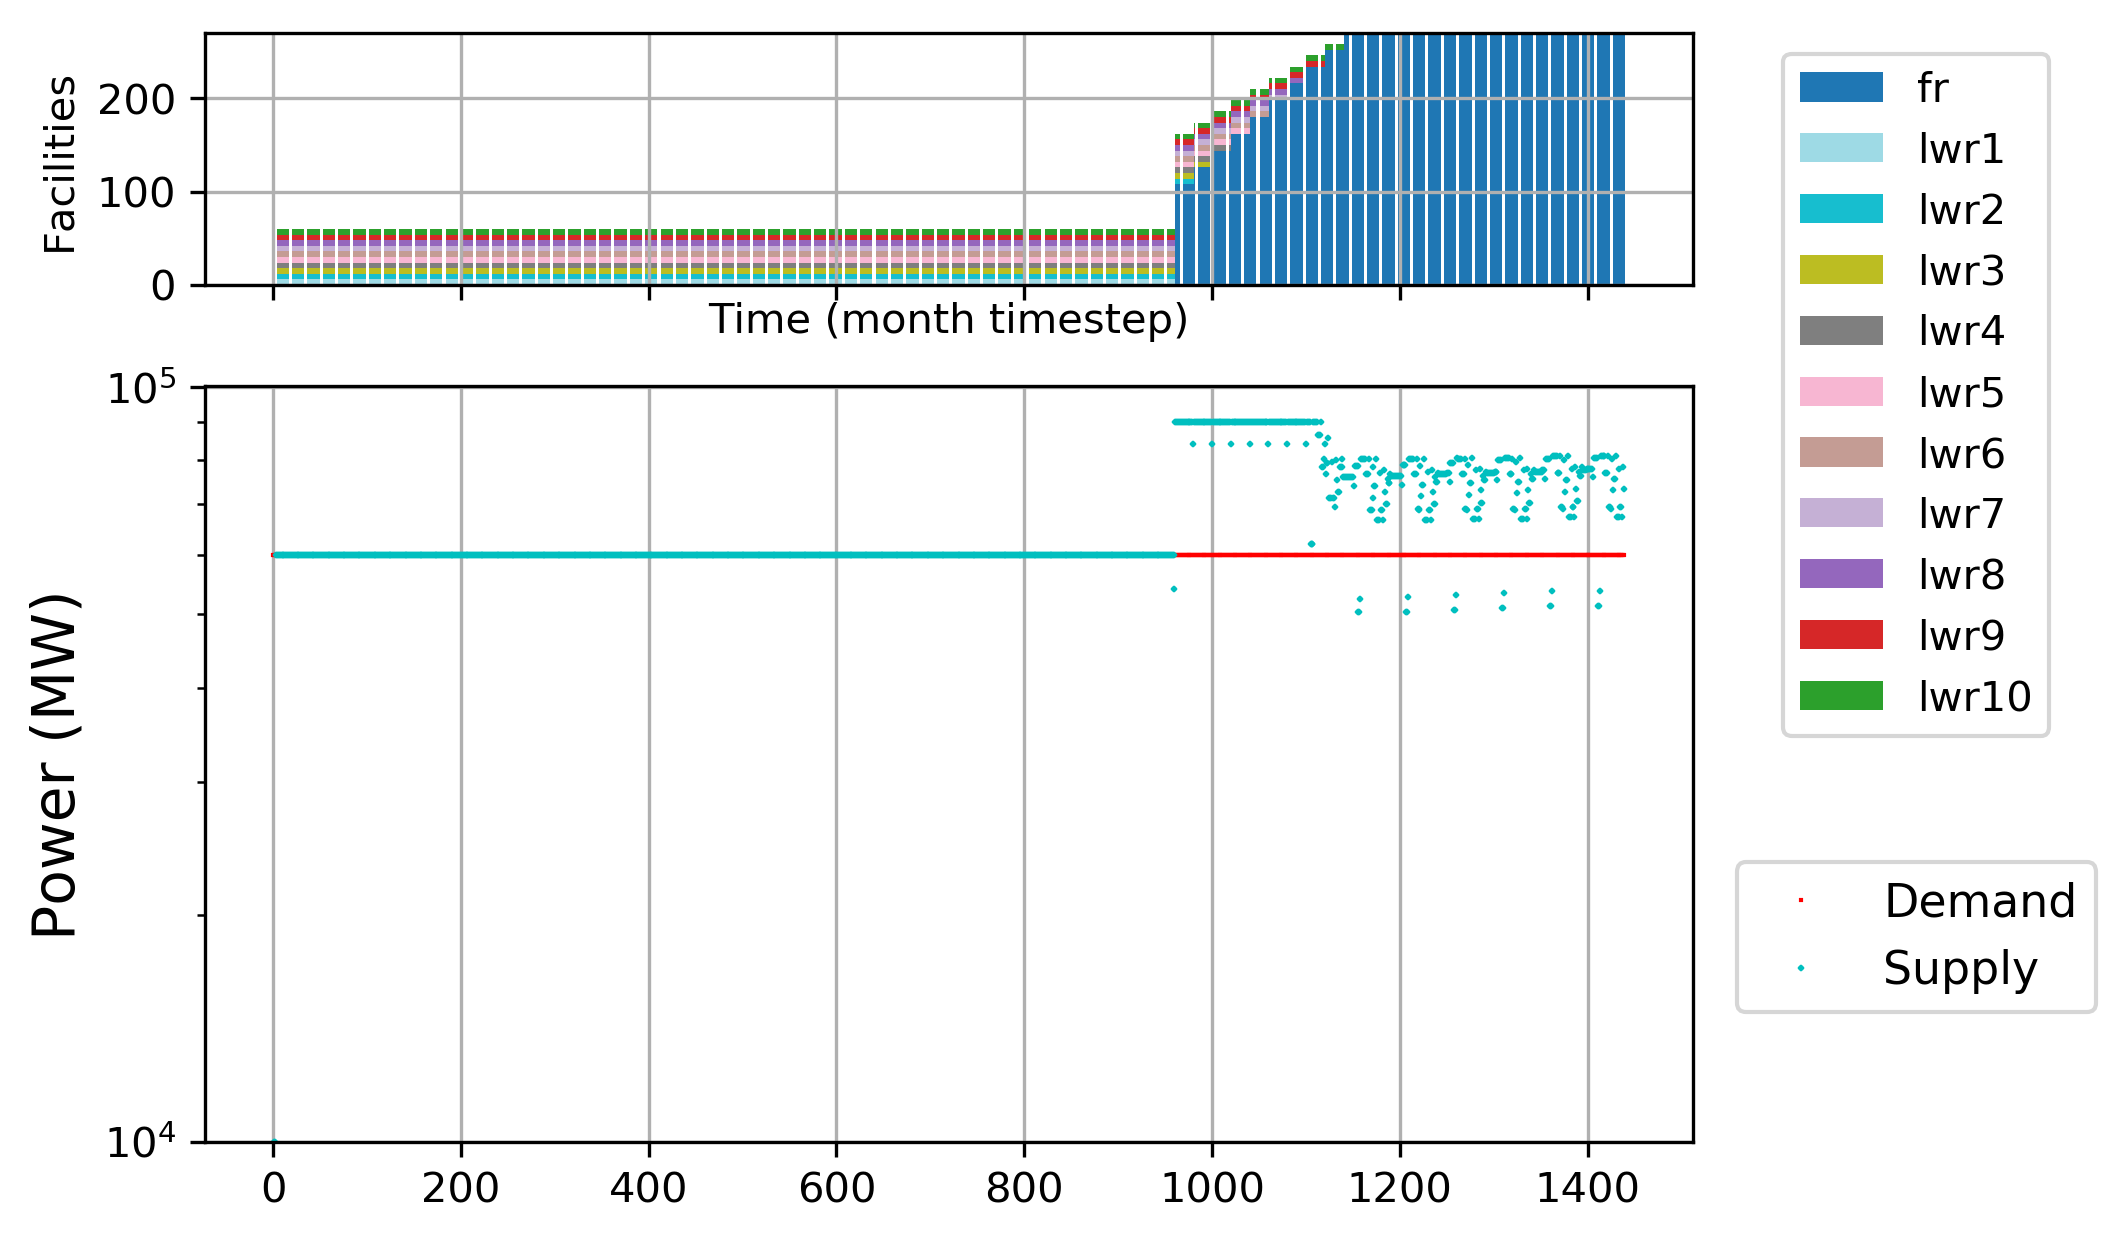
\includegraphics[width=\textwidth]{23-figures/0-poly-power.png} 
	\hfill
	\caption{Supply and demand of the commodity power.}
	\label{fig:23-power}
\end{figure}

\begin{figure}[H]
	\centering
	\begin{subfigure}[]{0.45\textwidth}
		\centering
		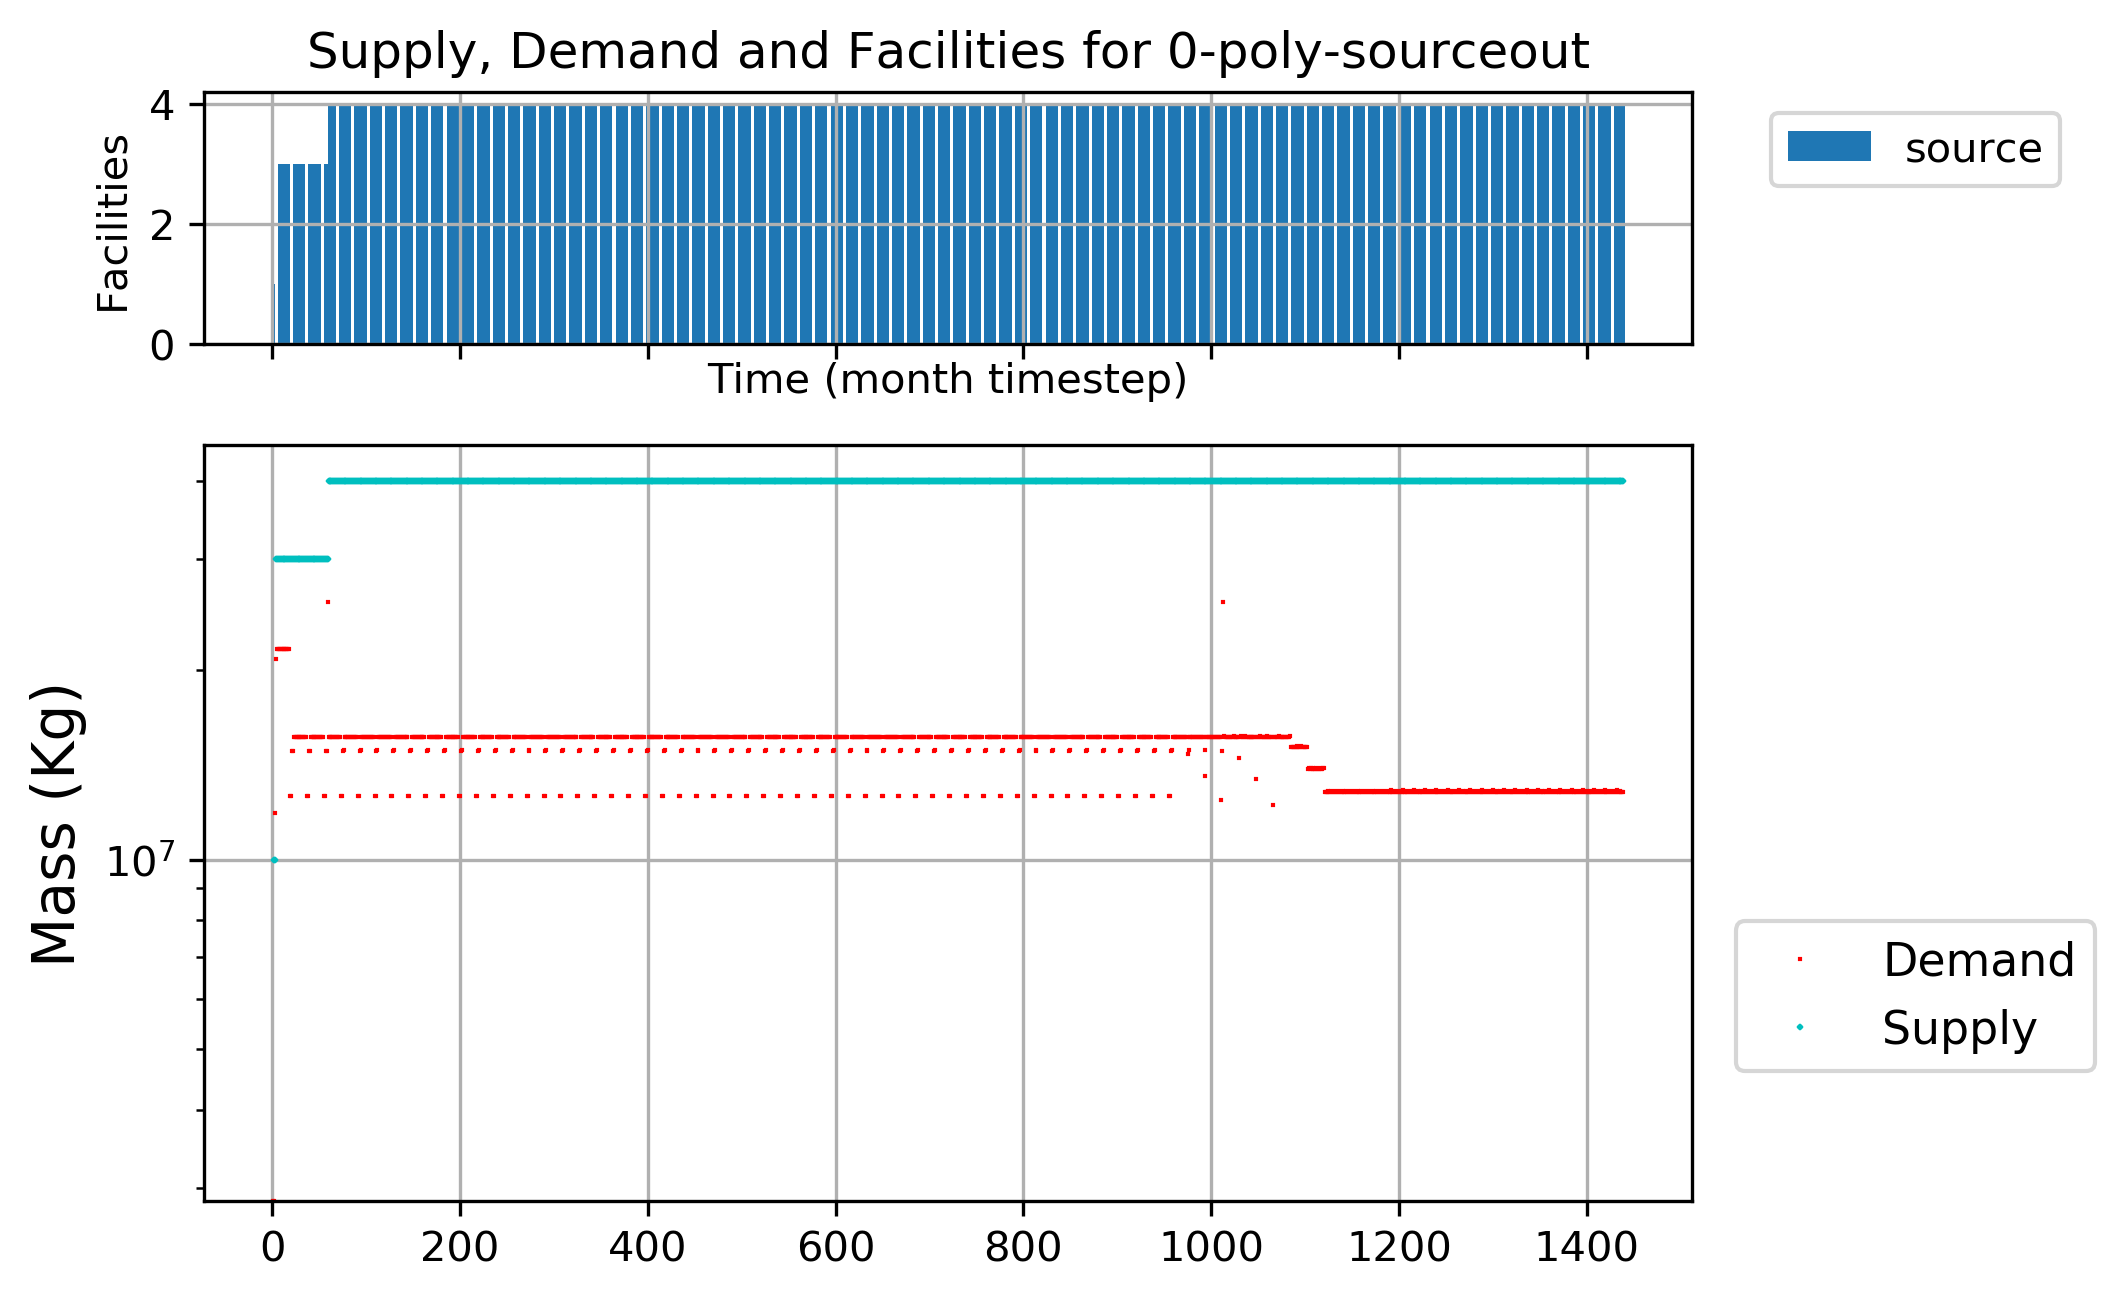
\includegraphics[width=\linewidth]{23-figures/0-poly-sourceout.png} 
		\caption{Commodity sourceout.}
		\label{fig:23-sourceout}
	\end{subfigure}
	\vspace{1cm}
	\begin{subfigure}[]{0.45\textwidth}
		\centering
		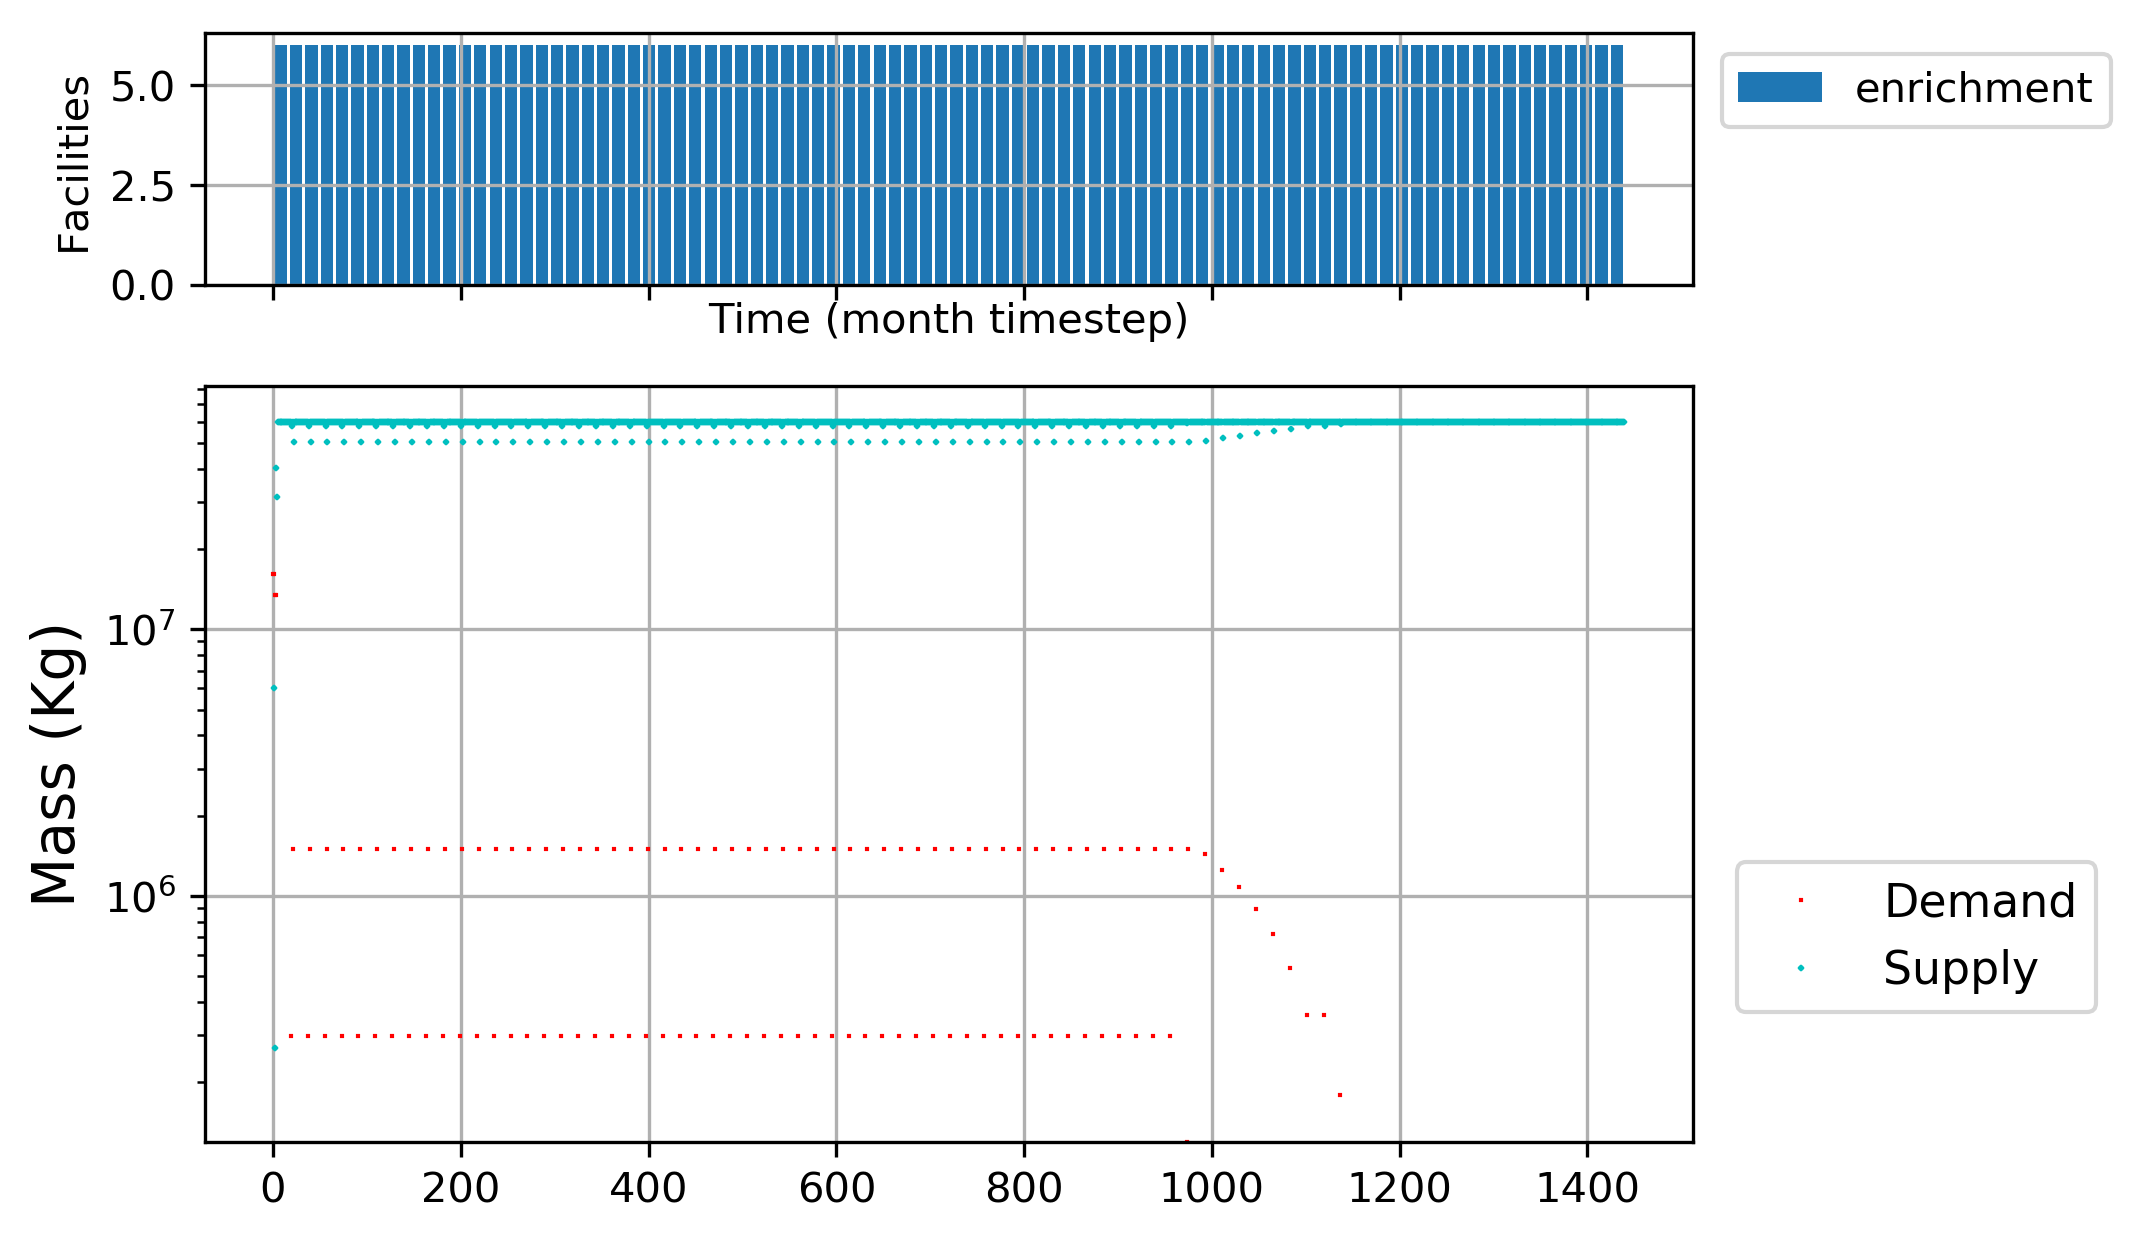
\includegraphics[width=\linewidth]{23-figures/0-poly-enrichmentout.png} 
		\caption{Commodity enrichmentout.}
		\label{fig:23-enrichmentout}
	\end{subfigure}
	\hfill
	\caption{Supply and demand of different commodities for the prediction method poly.}
	\label{fig:23-front}
\end{figure}

\begin{figure}[H]
	\centering
	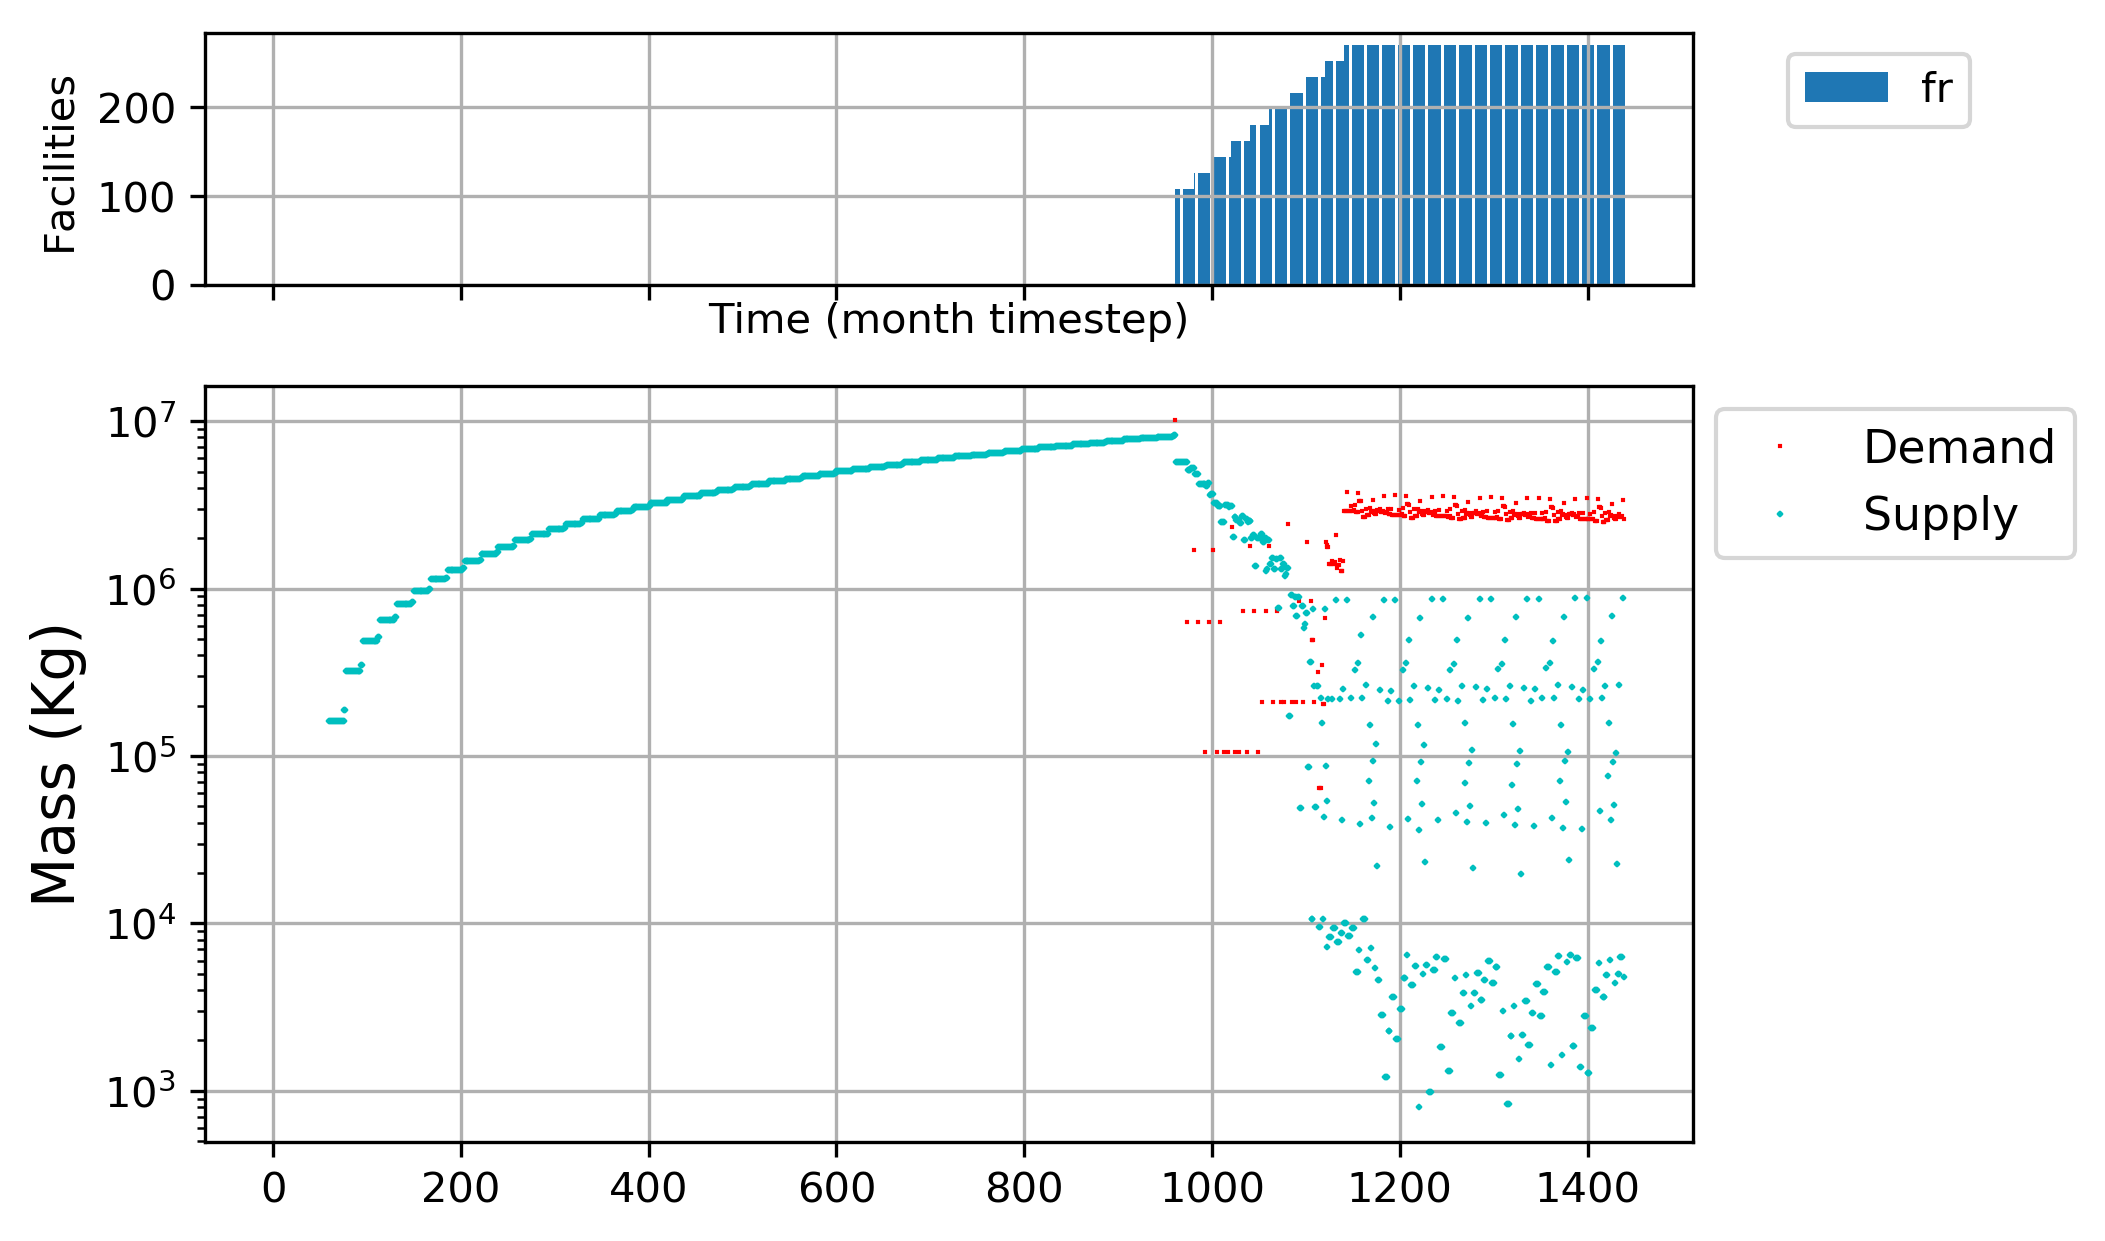
\includegraphics[width=\textwidth]{23-figures/0-poly-mixerout.png} 
	\hfill
	\caption{Supply and demand of the commodity mixerout.}
	\label{fig:23-mixerout}
\end{figure}

\begin{figure}[H]
	\centering
	\begin{subfigure}[]{0.45\textwidth}
		\centering
		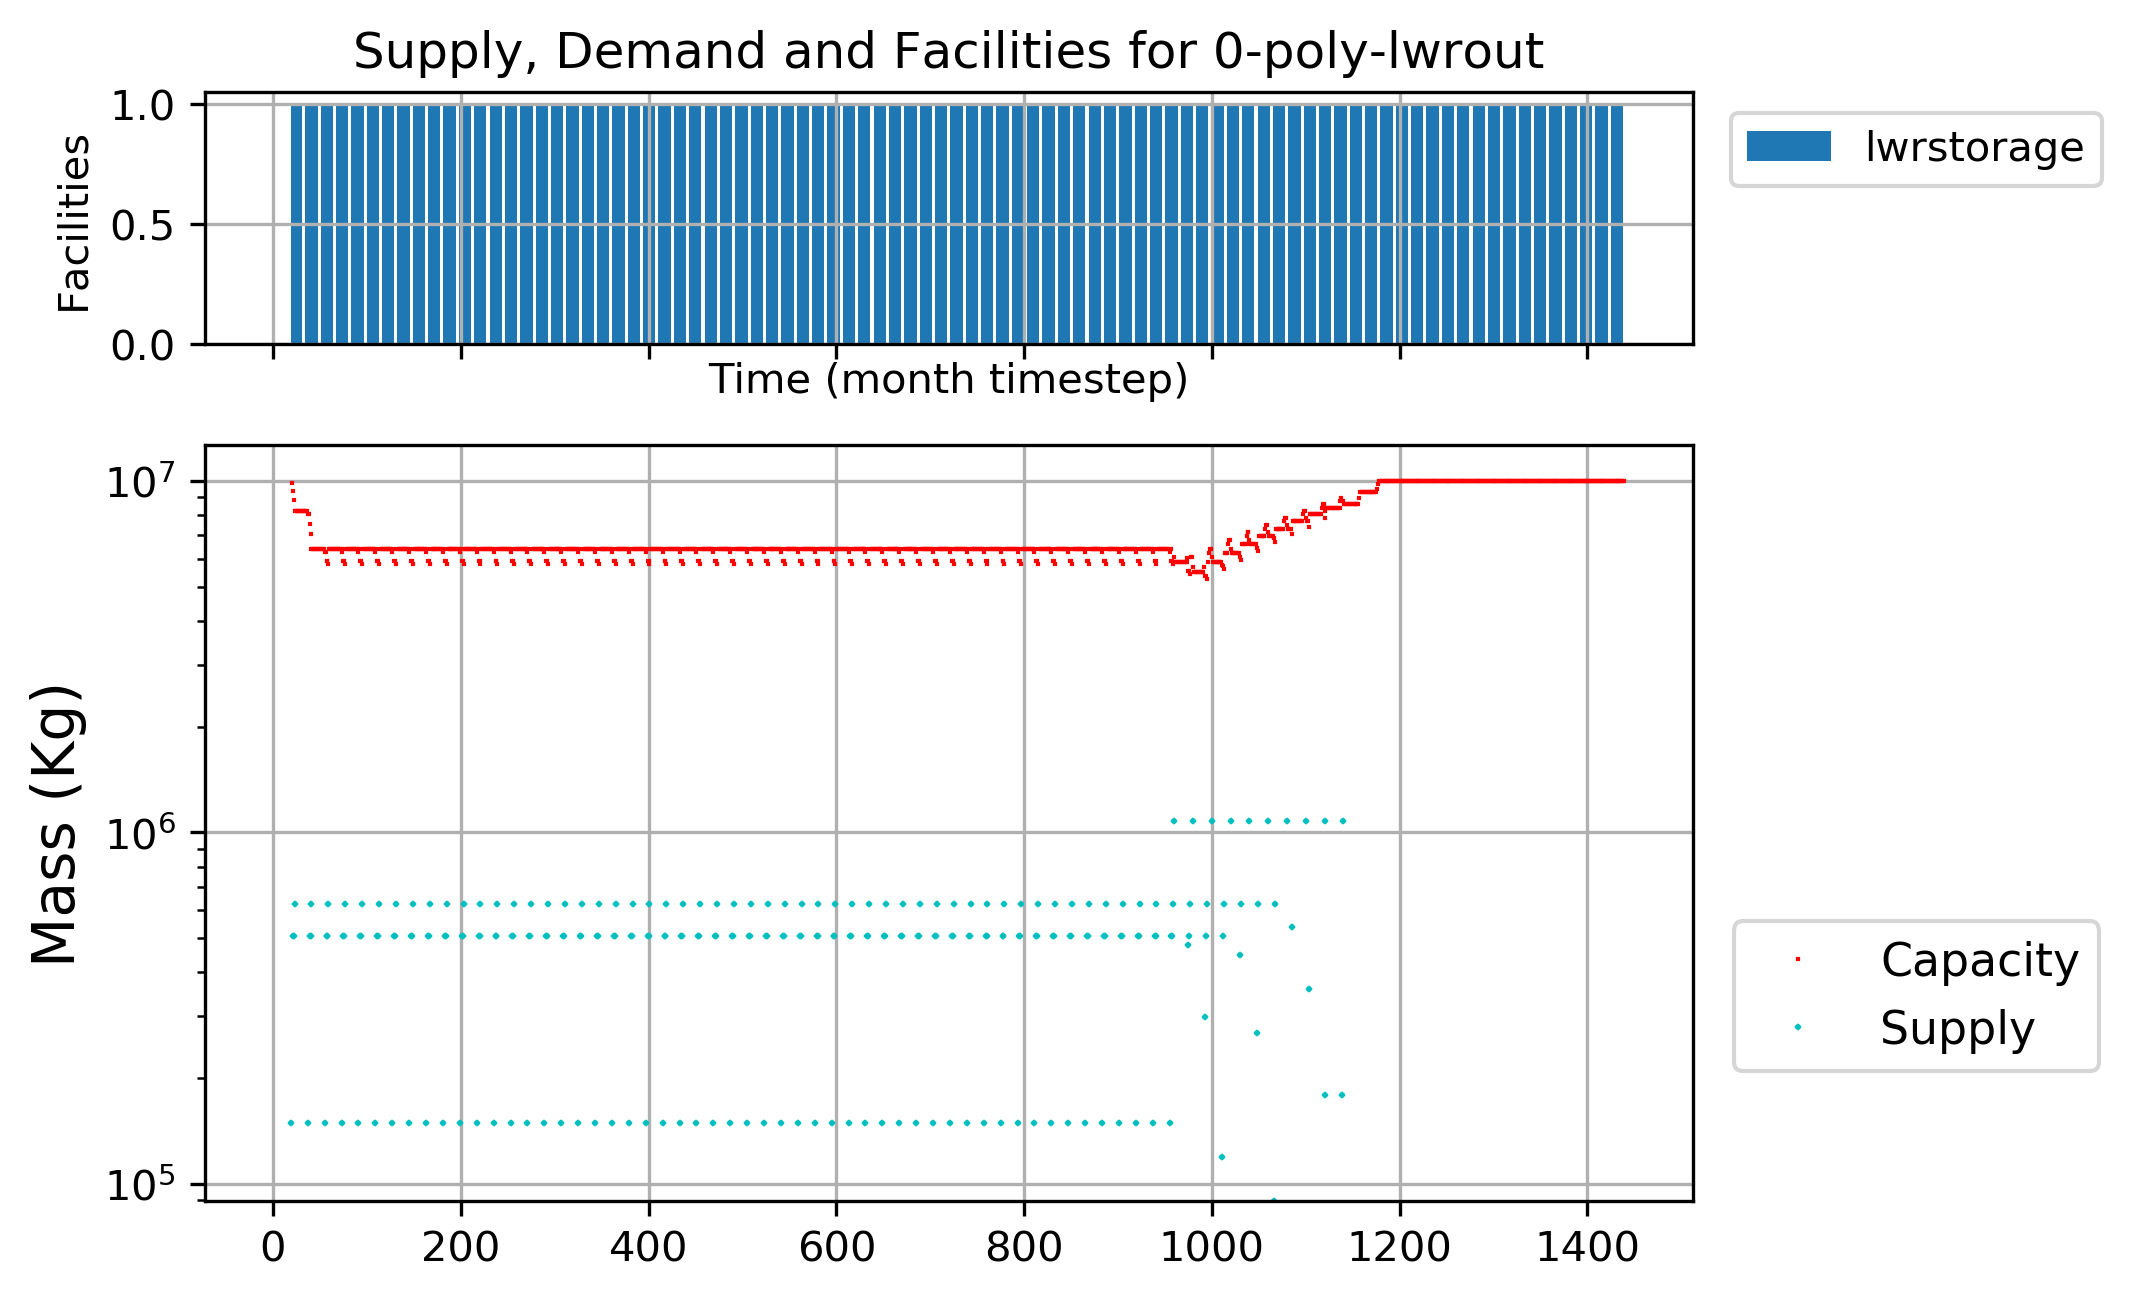
\includegraphics[width=\linewidth]{23-figures/0-poly-lwrout.png} 
		\caption{Commodity lwrout.}
		\label{fig:23-lwrout}
	\end{subfigure}
	\vspace{1cm}
	\begin{subfigure}[]{0.45\textwidth}
		\centering
		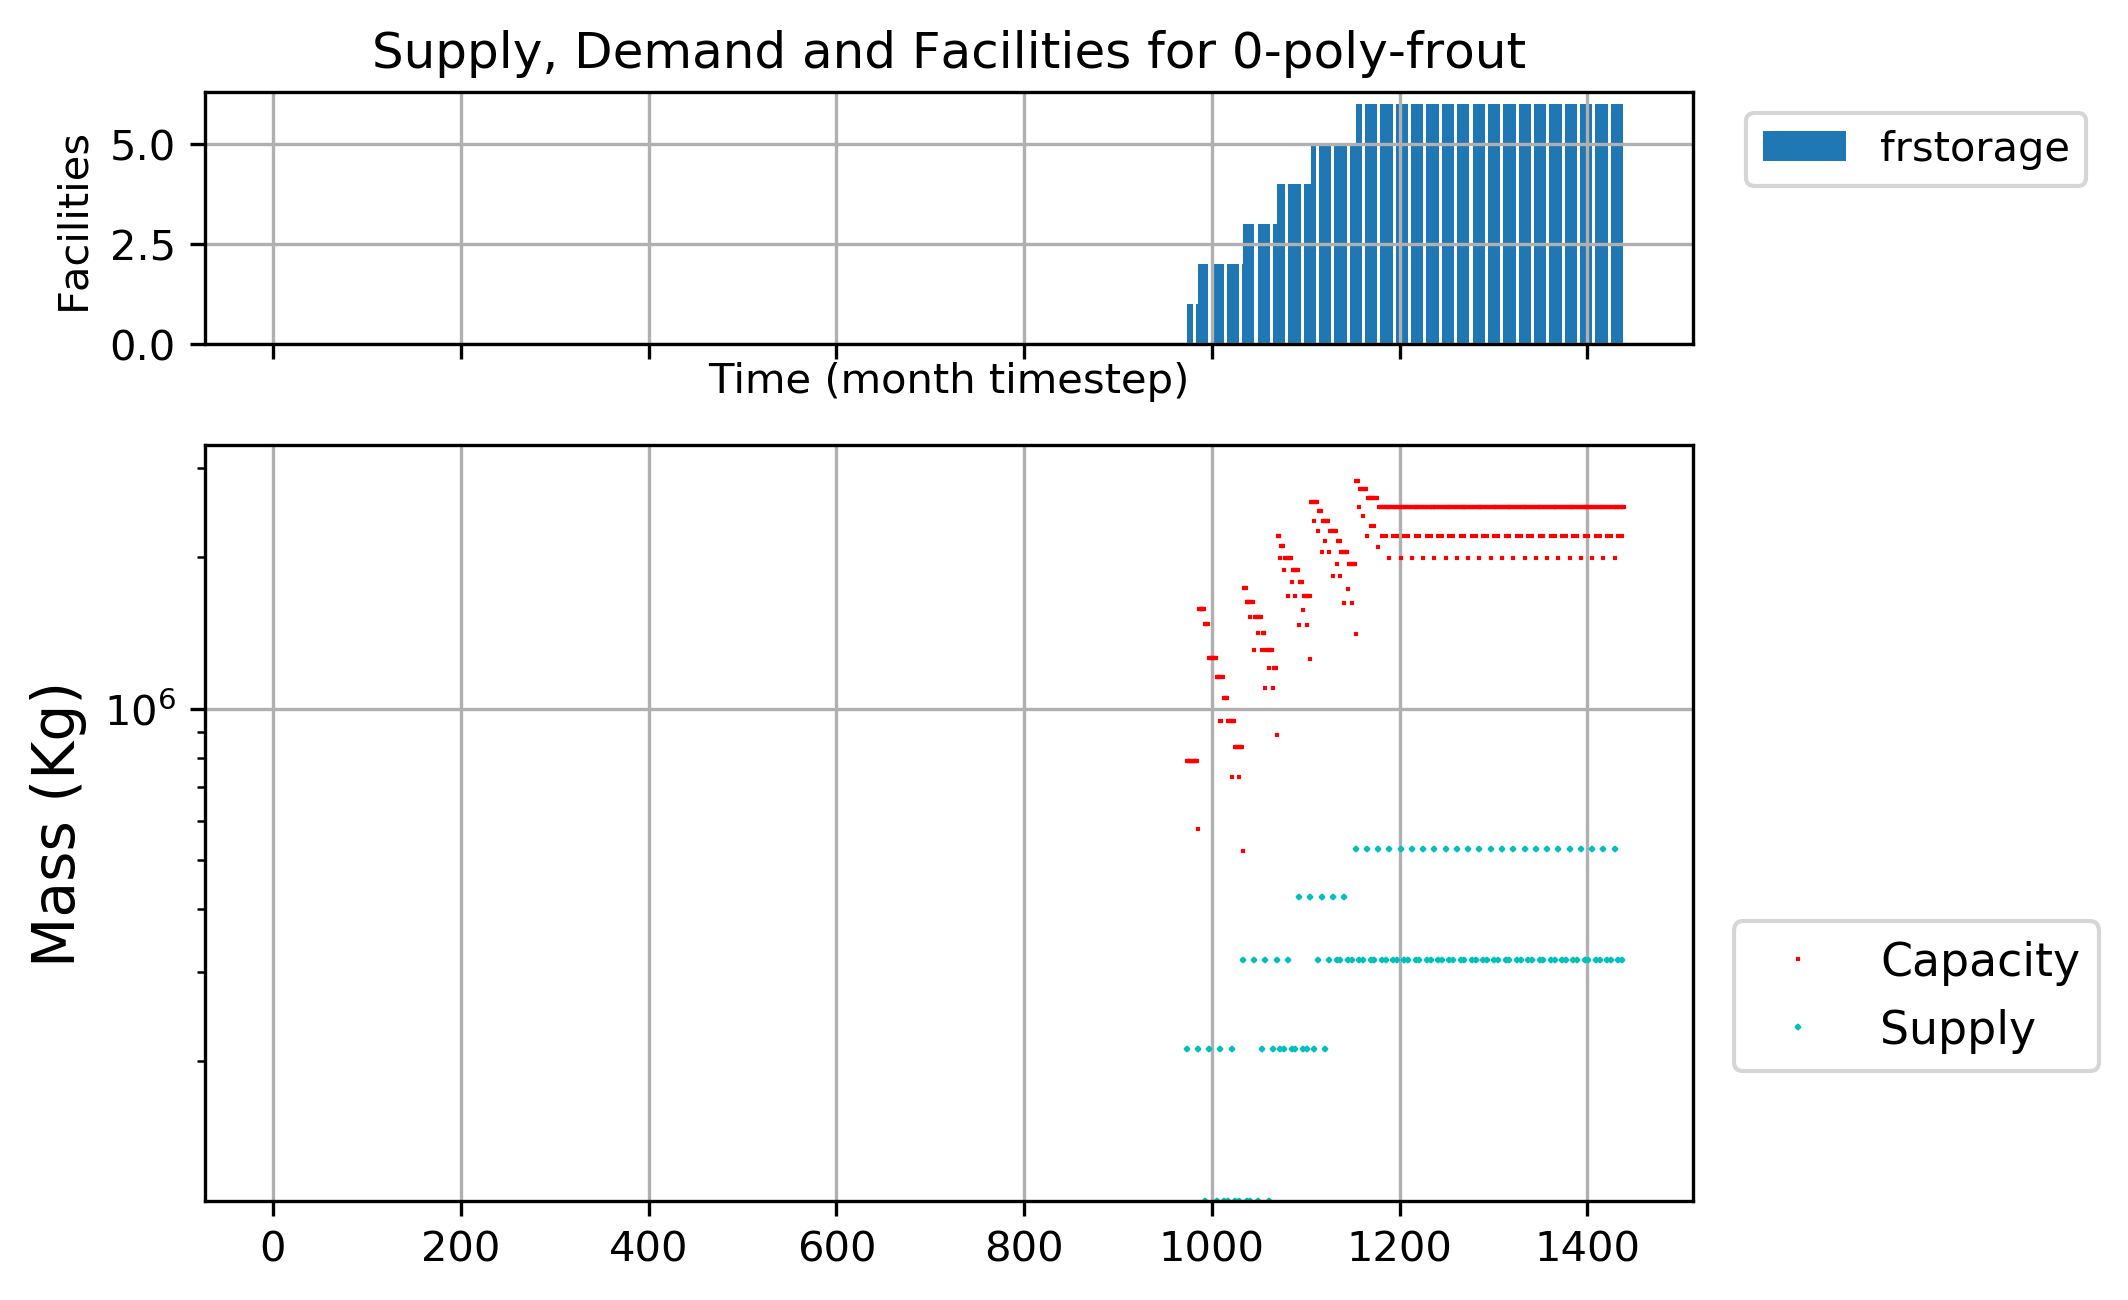
\includegraphics[width=\linewidth]{23-figures/0-poly-frout.png} 
		\caption{Commodity frout.}
		\label{fig:23-frout}
	\end{subfigure}
	\hfill
	\caption{Supply and demand of different commodities for the prediction method poly.}
	\label{fig:23-out}
\end{figure}

\begin{figure}[H]
	\centering
	\begin{subfigure}[t]{0.45\textwidth}
		\centering
		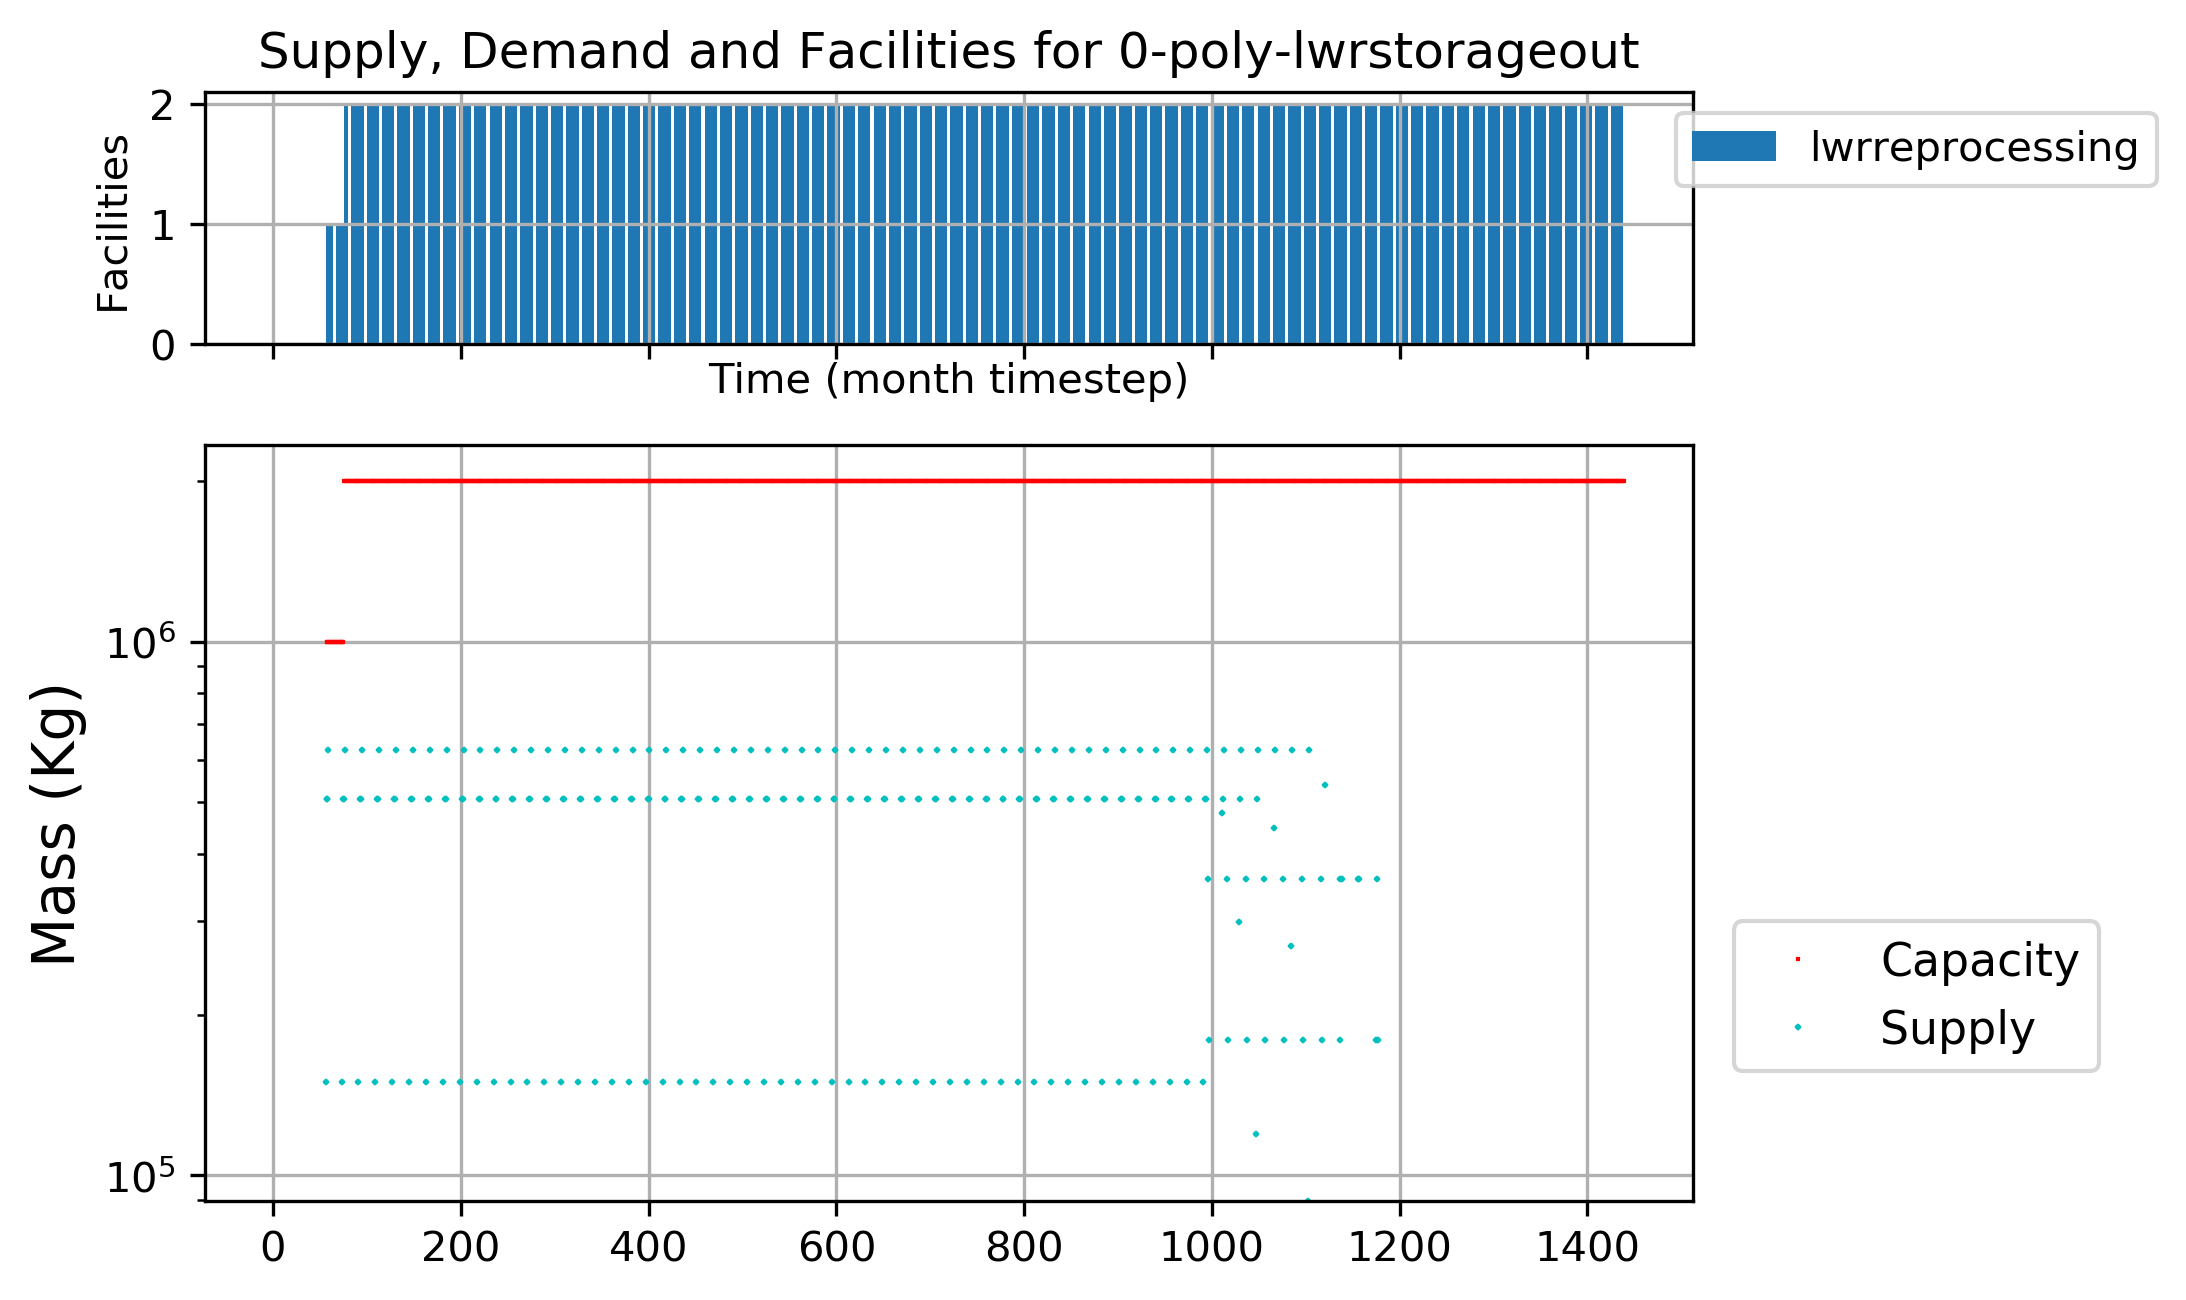
\includegraphics[width=\linewidth]{23-figures/0-poly-lwrstorageout.png} 
		\caption{Commodity lwrstorageout.}
		\label{fig:23-lwrstorageout}
	\end{subfigure}
	\vspace{1cm}
	\begin{subfigure}[t]{0.45\textwidth}
		\centering
		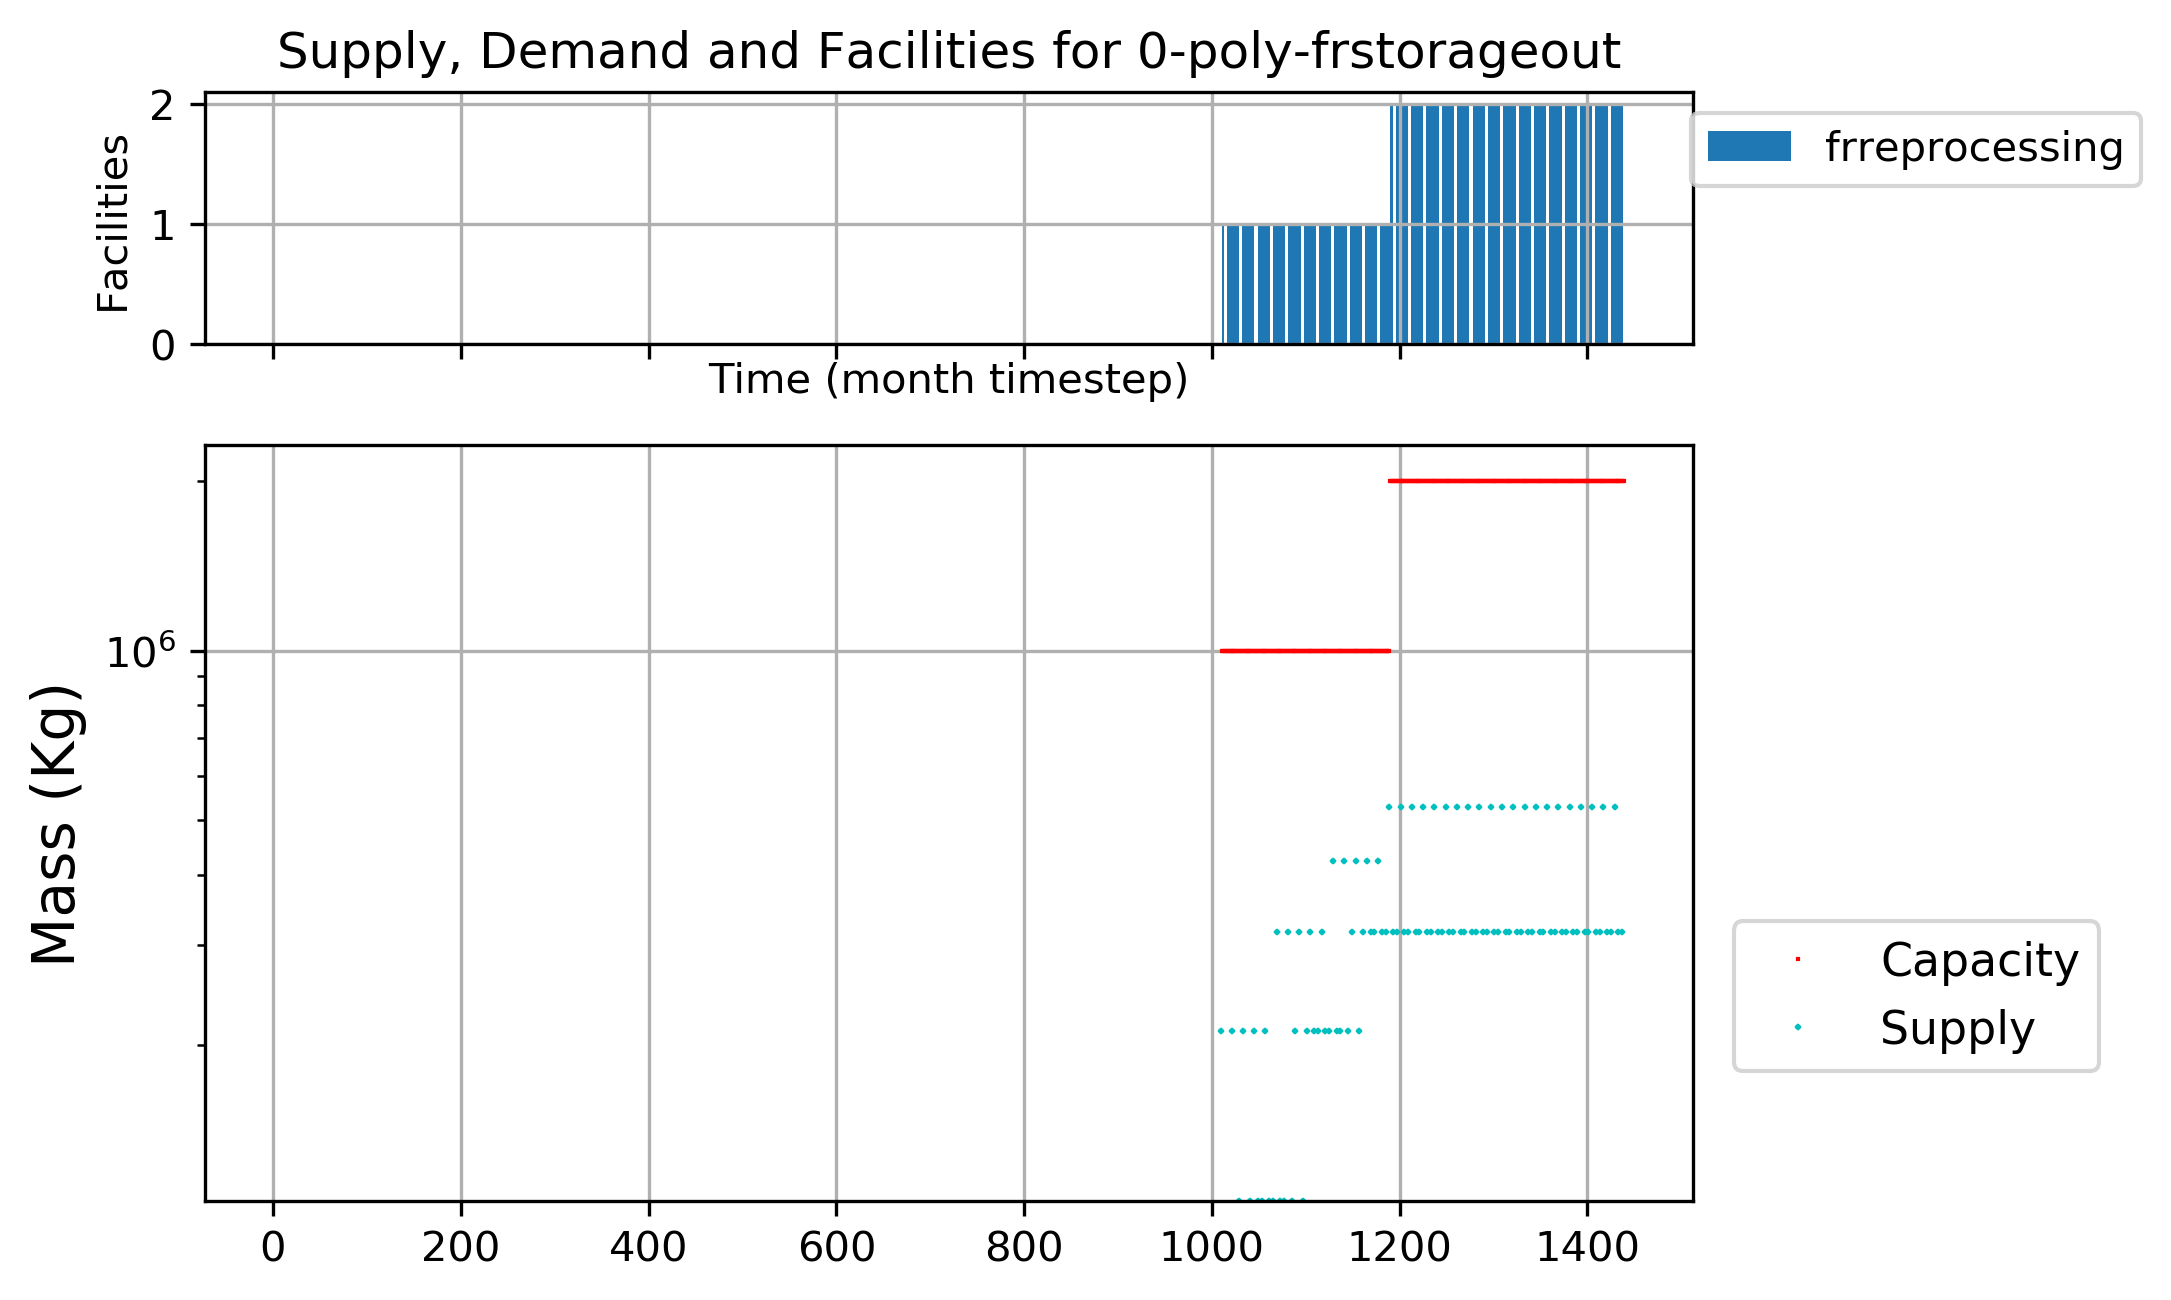
\includegraphics[width=\linewidth]{23-figures/0-poly-frstorageout.png} 
		\caption{Commodity frstorageout.}
		\label{fig:23-frstorageout}
	\end{subfigure}
	\hfill
	\caption{Supply and demand of different commodities for the prediction method poly.}
	\label{fig:23-storageout}
\end{figure}

\begin{figure}[H]
	\centering
	\begin{subfigure}[t]{0.45\textwidth}
		\centering
		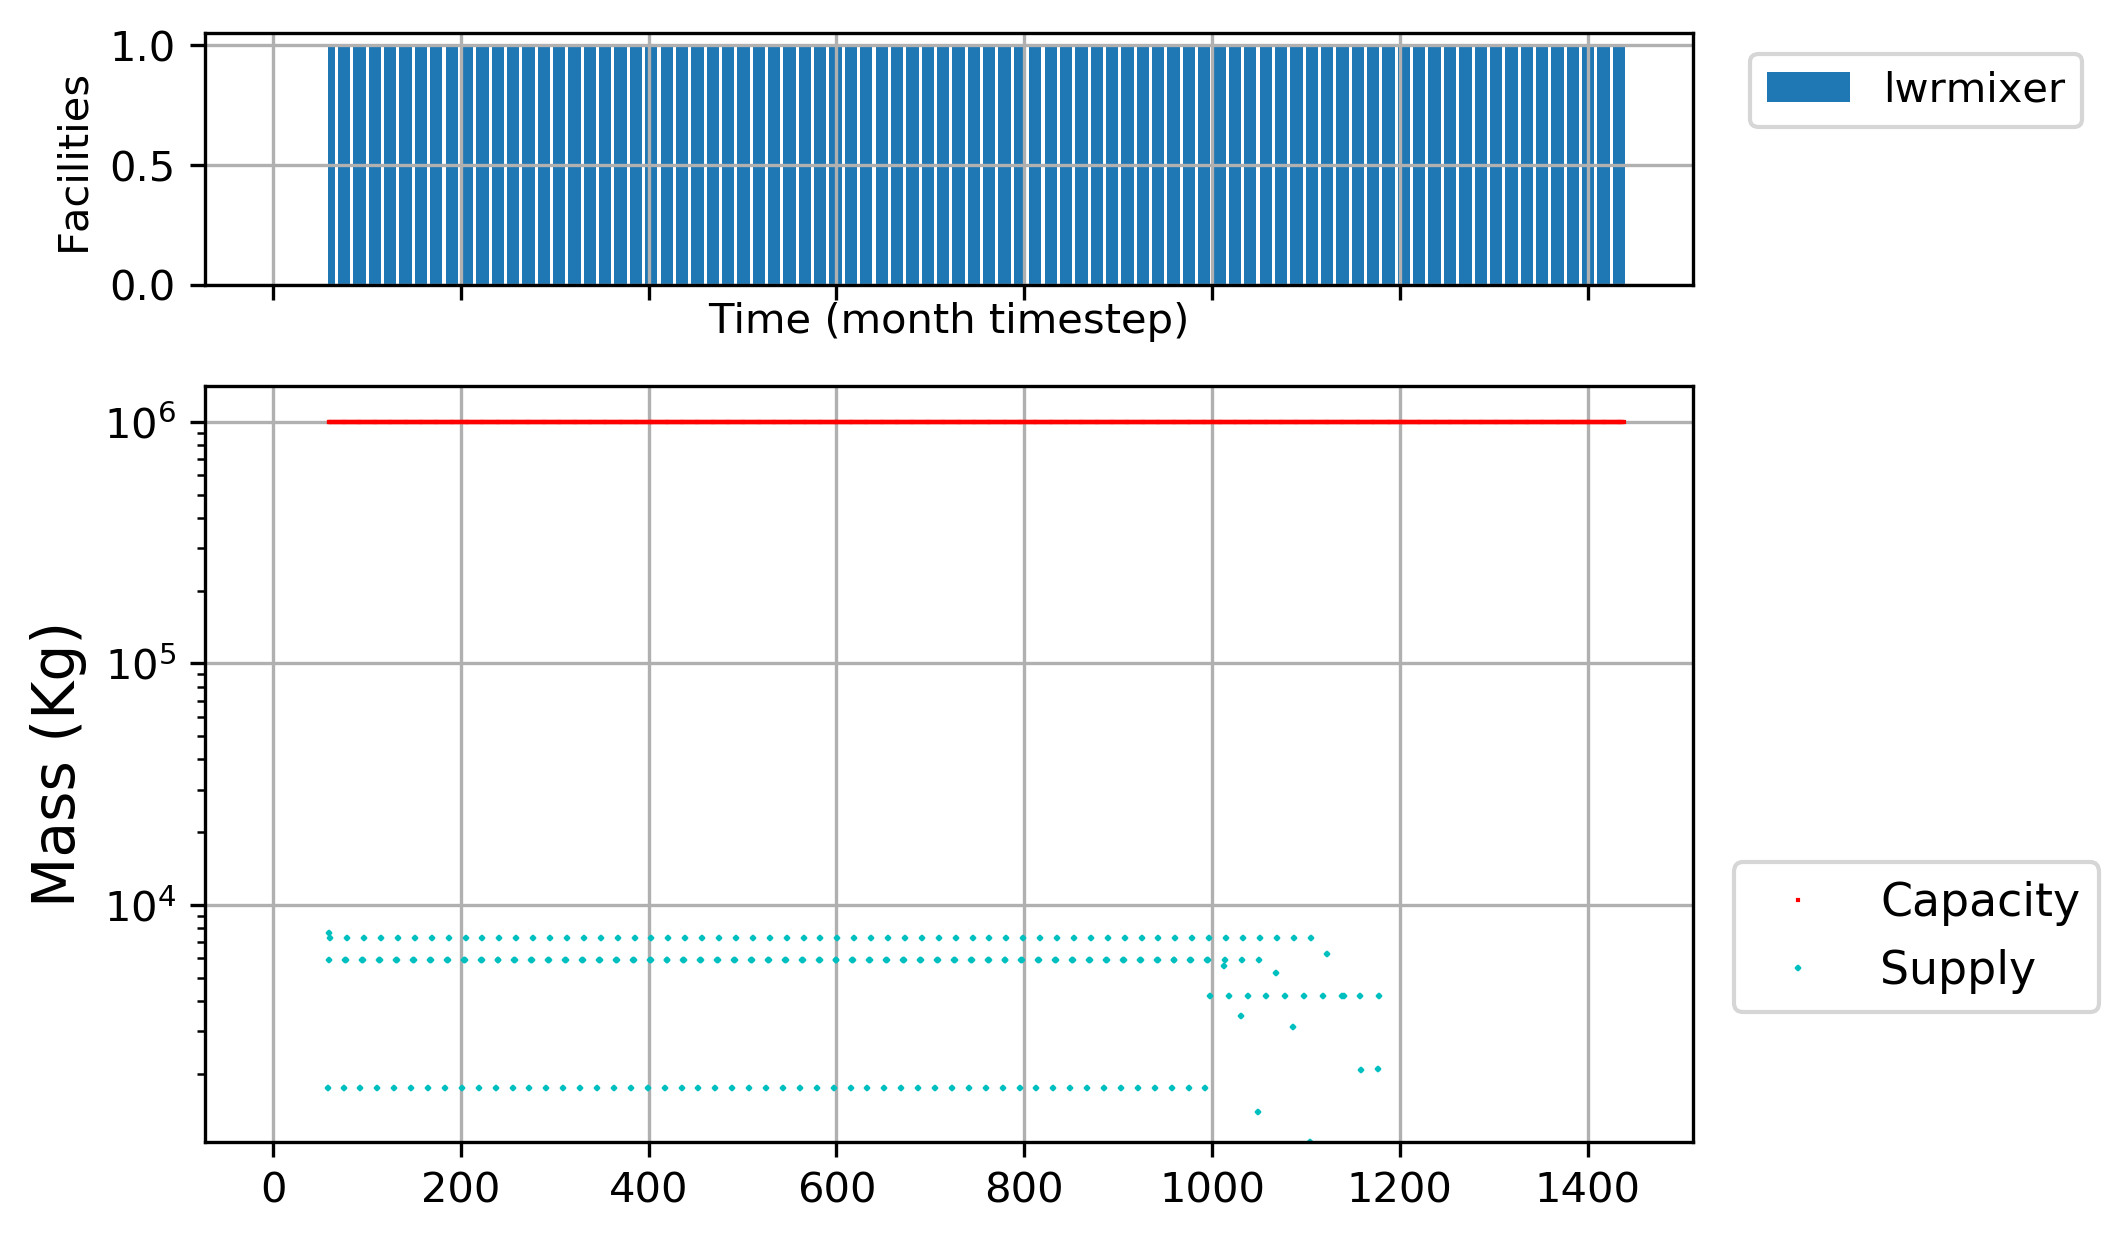
\includegraphics[width=\linewidth]{23-figures/0-poly-lwrpu.png} 
		\caption{Commodity lwrpu.}
		\label{fig:23-lwrpu}
	\end{subfigure}
	\vspace{1cm}
	\begin{subfigure}[t]{0.45\textwidth}
		\centering
		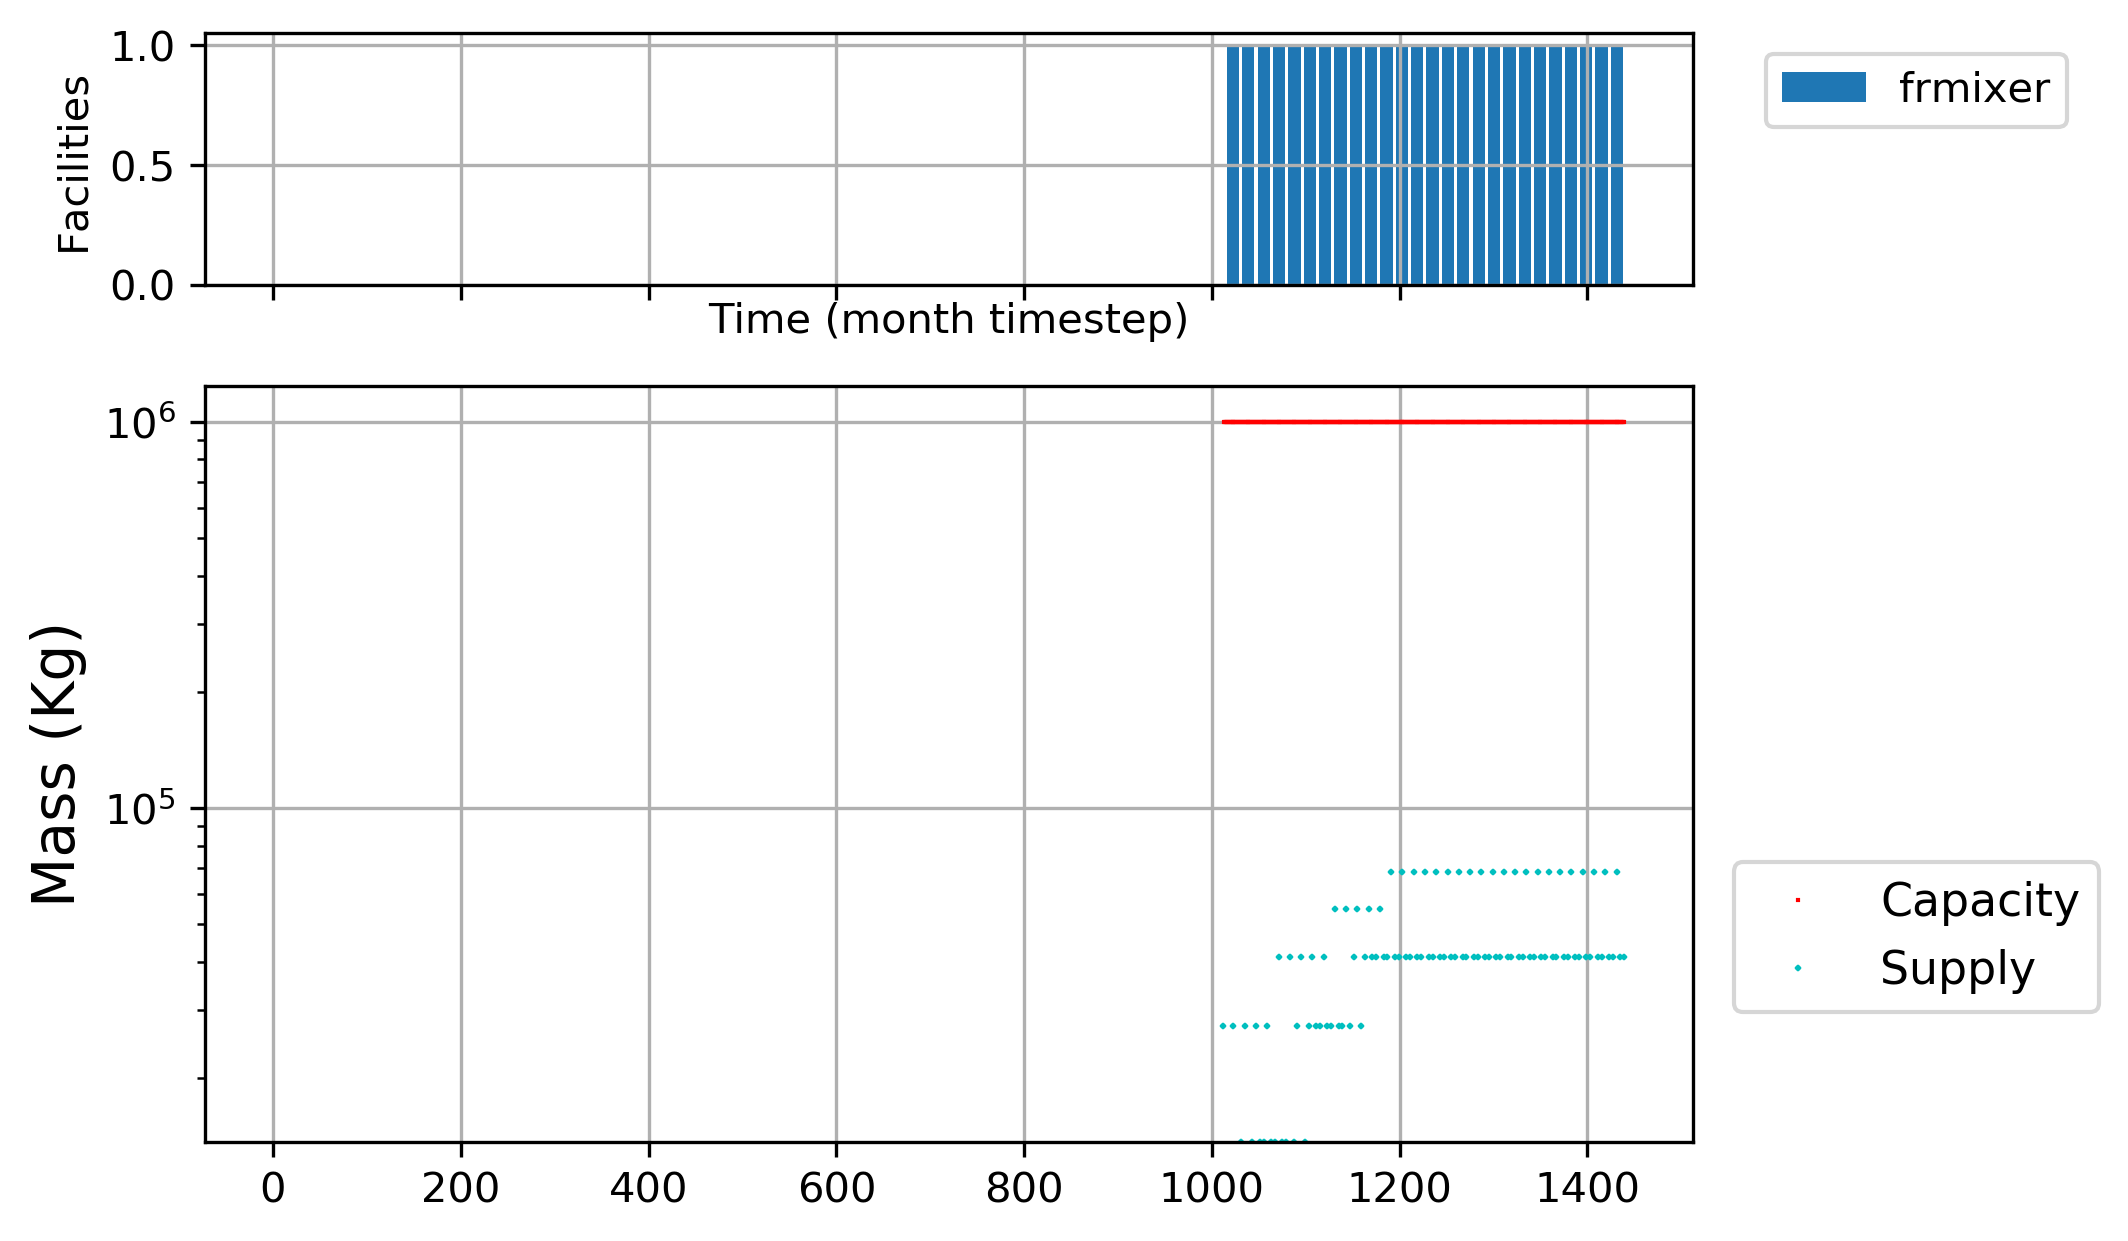
\includegraphics[width=\linewidth]{23-figures/0-poly-frpu.png} 
		\caption{Commodity frpu.}
		\label{fig:23-frpu}
	\end{subfigure}
	\hfill
	\caption{Supply and demand of different commodities for the prediction method poly.}
	\label{fig:23-pu}
\end{figure}

\begin{figure}[H]
	\centering
	\begin{subfigure}[t]{0.45\textwidth}
		\centering
		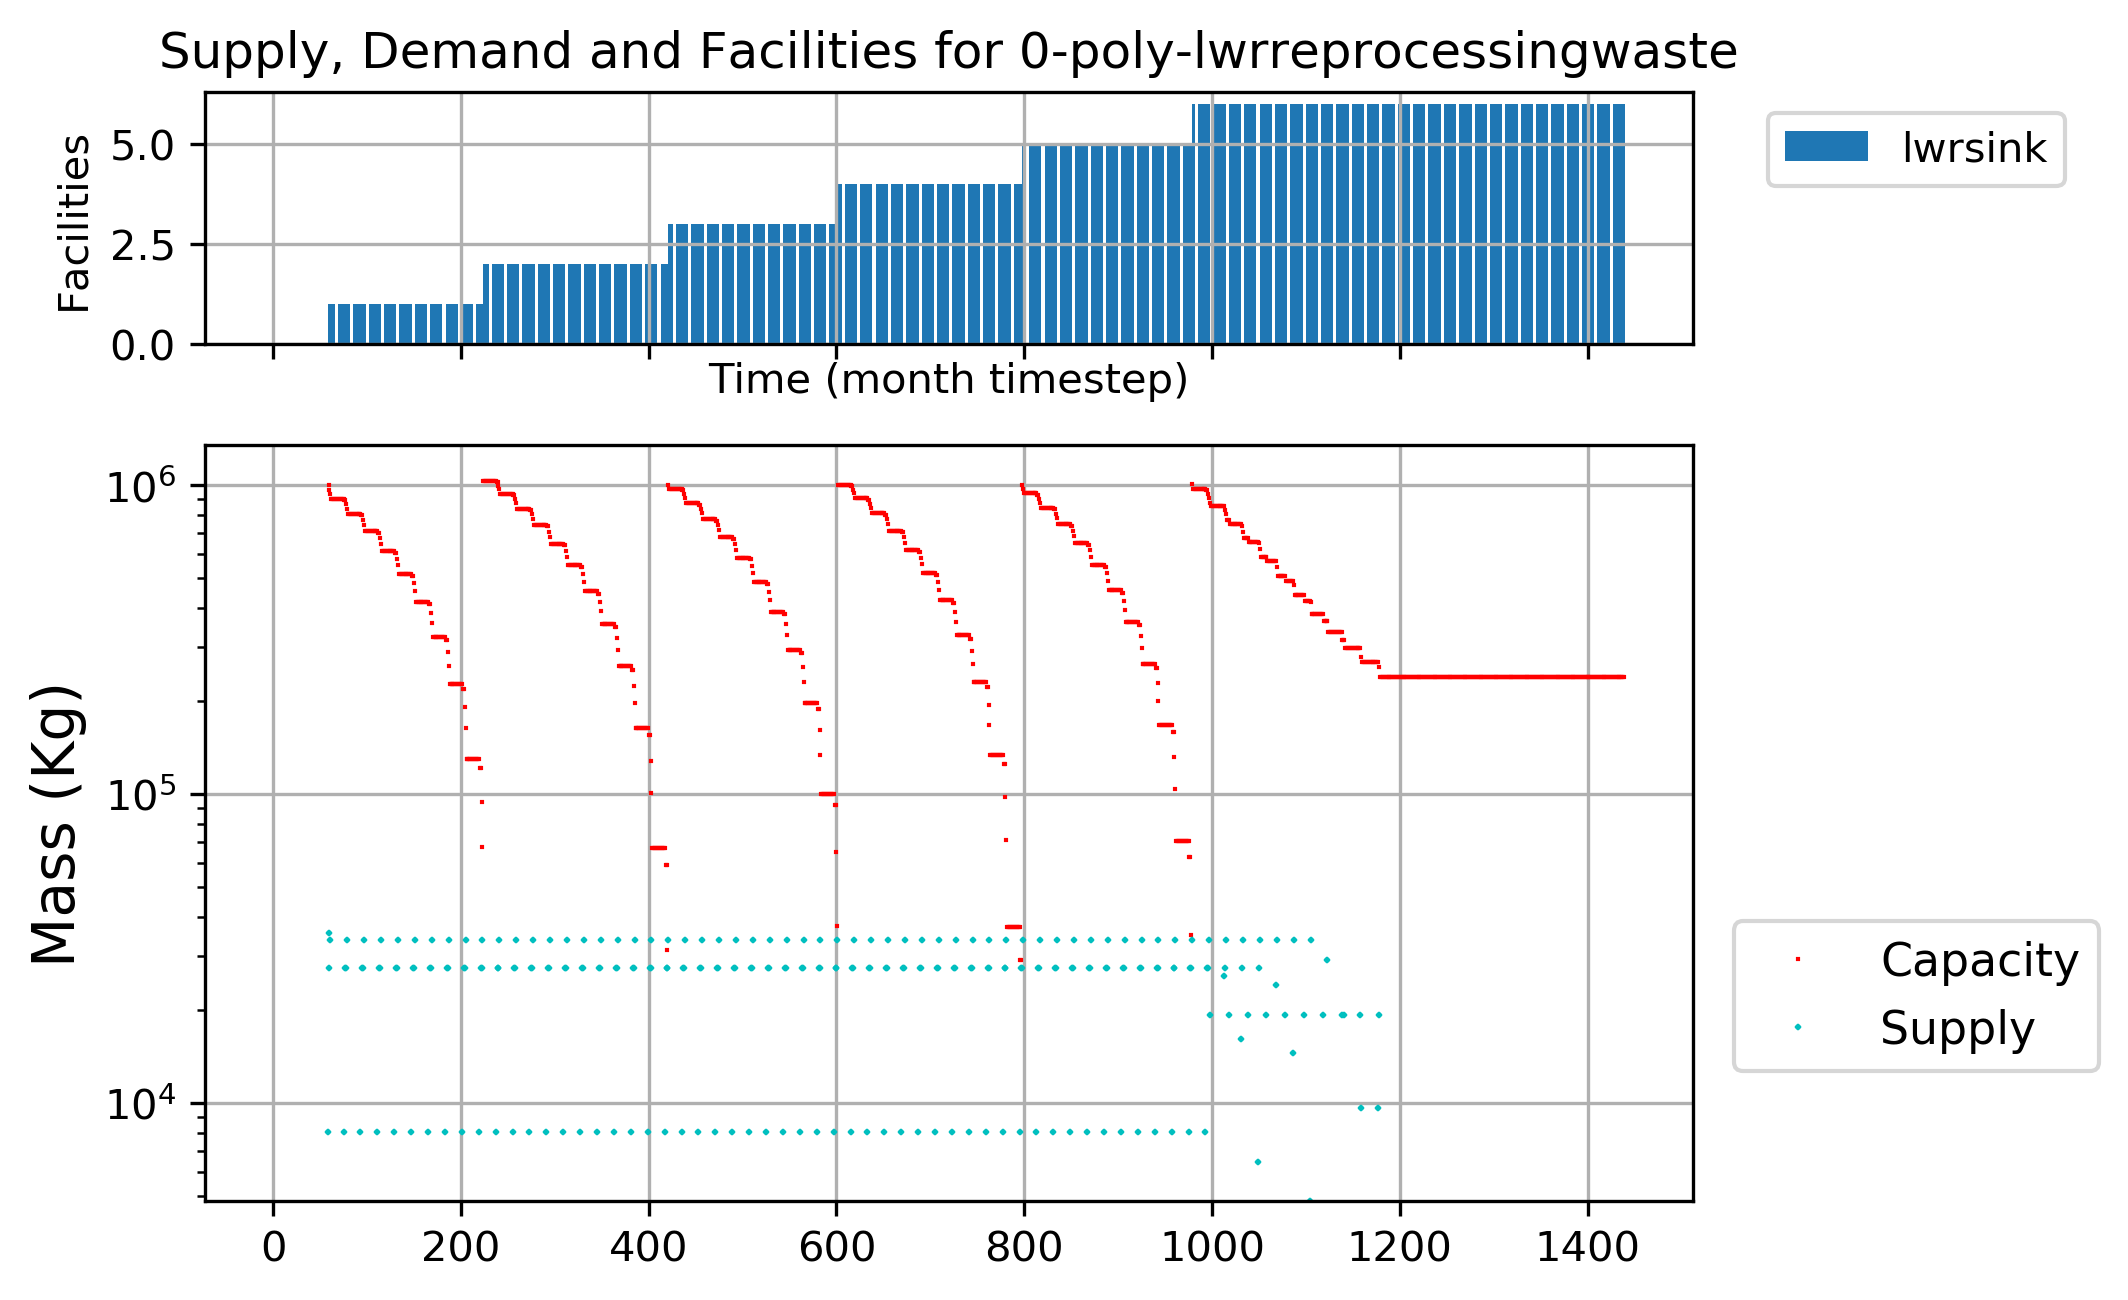
\includegraphics[width=\linewidth]{23-figures/0-poly-lwrreprocessingwaste.png} 
		\caption{Commodity lwrreprocessingwaste.}
		\label{fig:23-lwrreprocessingwaste}
	\end{subfigure}
	\vspace{1cm}
	\begin{subfigure}[t]{0.45\textwidth}
		\centering
		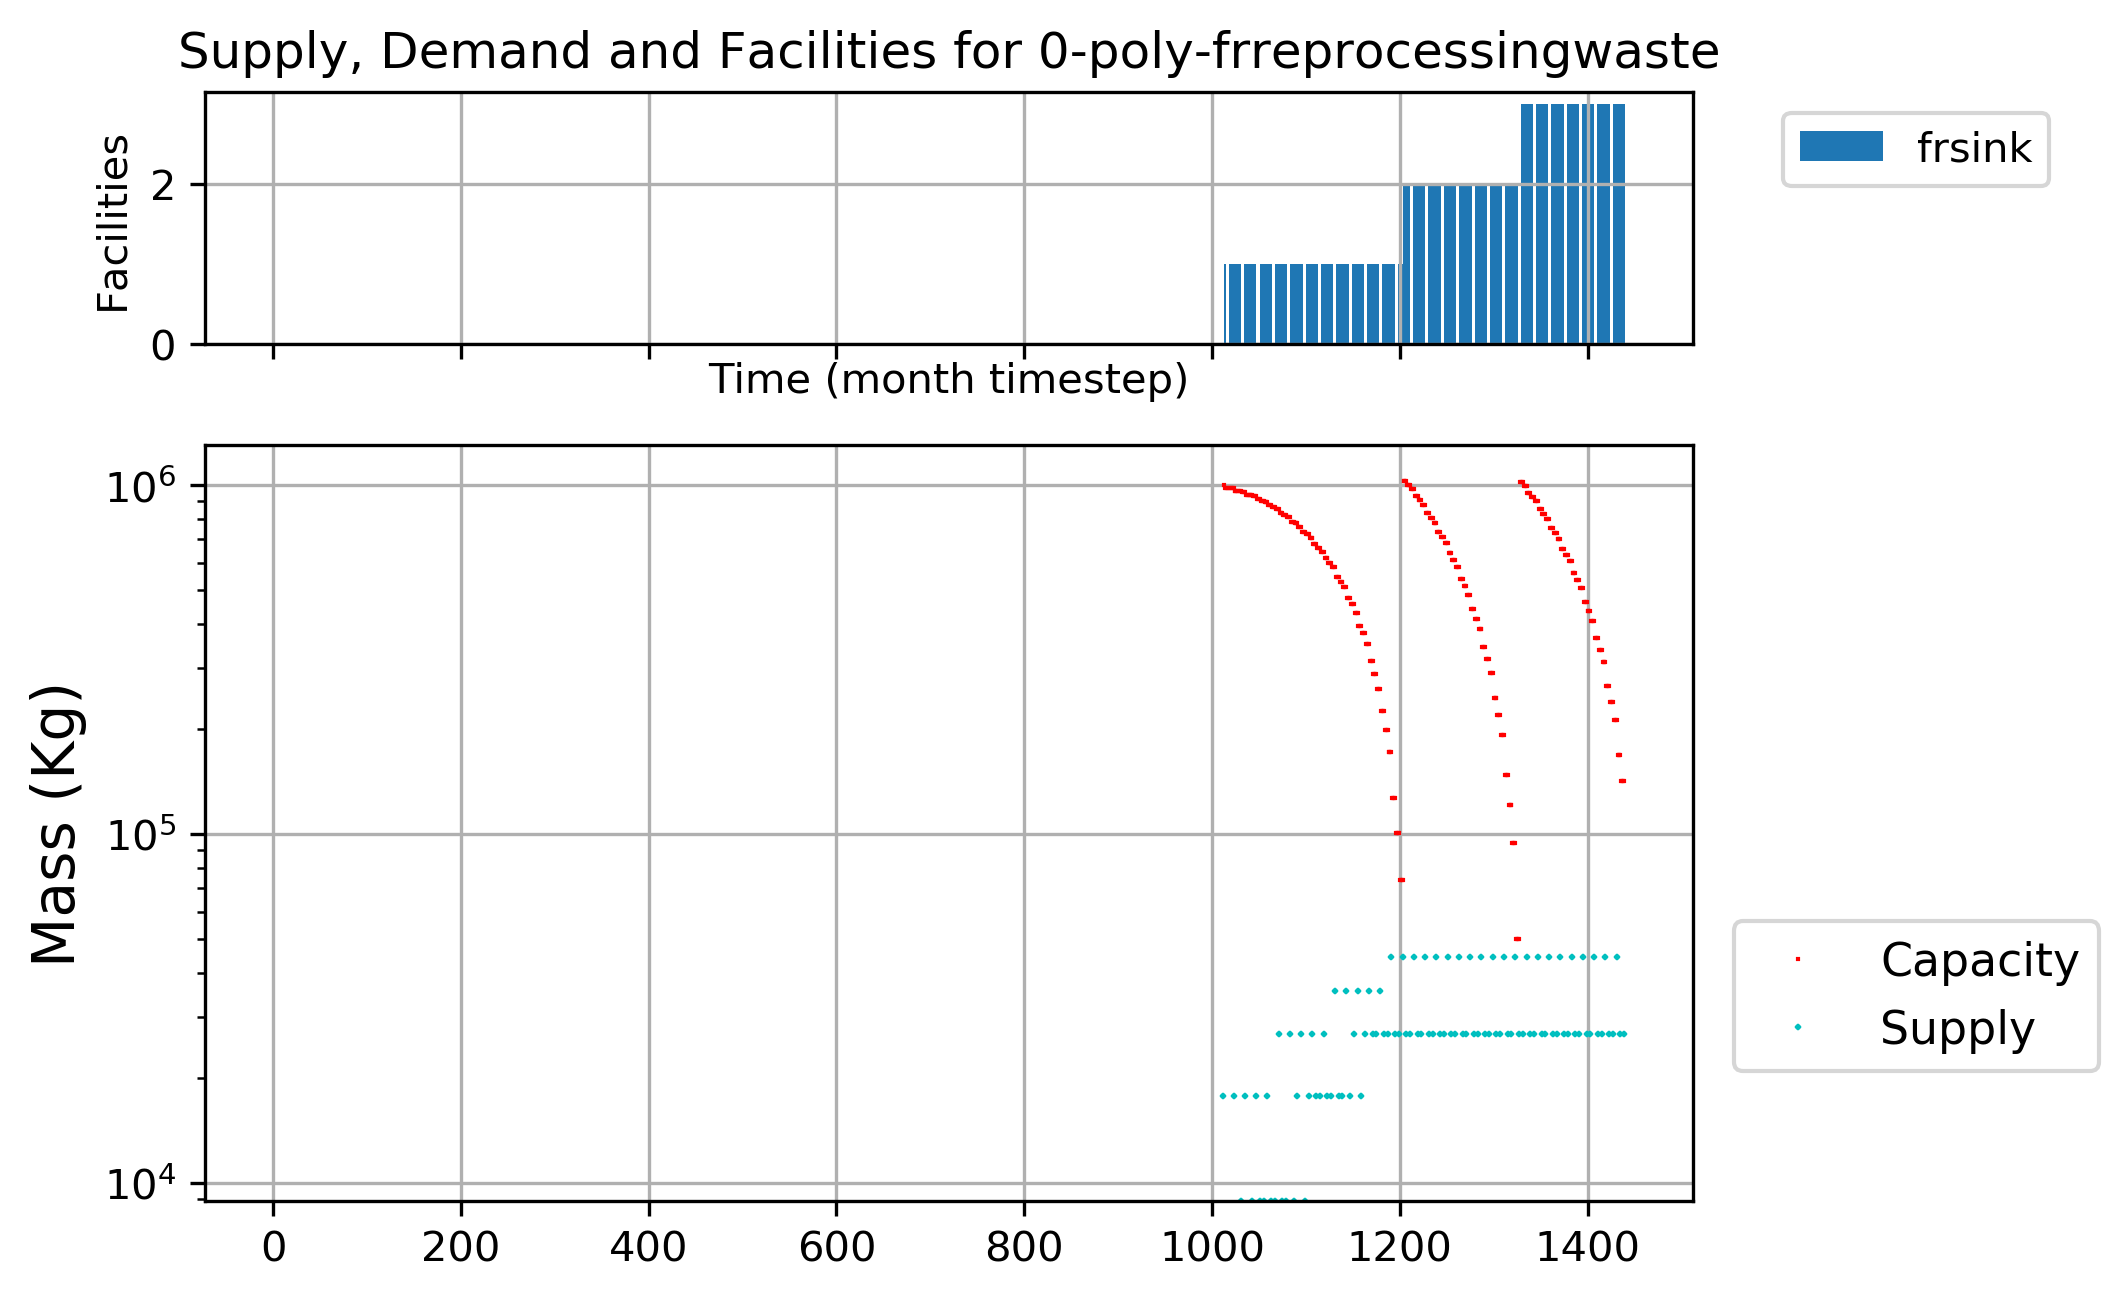
\includegraphics[width=\linewidth]{23-figures/0-poly-frreprocessingwaste.png} 
		\caption{Commodity frreprocessingwaste.}
		\label{fig:23-frreprocessingwaste}
	\end{subfigure}
	\hfill
	\caption{Supply and demand of different commodities for the prediction method poly.}
	\label{fig:23-waste}
\end{figure}

\begin{table}[H]
	\centering
	\caption{Undersupply and oversupply of different commodities using poly to calculate EG01-EG23.}
	\label{tab:23-commod}
	\begin{tabularx}{\textwidth}{lRRR}
		\hline
		Commodity & Undersupplied & Cumulative  & Cumulative \\
		& Timesteps     & Undersupply [$10^3$Kg]  & Oversupply [$10^6$Kg] \\ \hline
		sourceout & 2 & 4713.  &  35648   \\ 
		enrichmentout & 4 & 48.5$x 10^3$  &  42259   \\ 
		lwrout & 1 & 149 & - \\
		frout & 1 & 211 & - \\
		lwrstorageout & 1 & 149 & - \\
		frstorageout & 1 & 211 & - \\
        lwrpu & 1 & 1.7 & - \\
        frpu & 1 & 27.4 & - \\ \hline
	\end{tabularx}
\end{table}

\section{Eg01-Eg24}

Figure \ref{fig:24flow} shows the flow of Eg01-Eg24.

\begin{figure}[H]
	\centering
	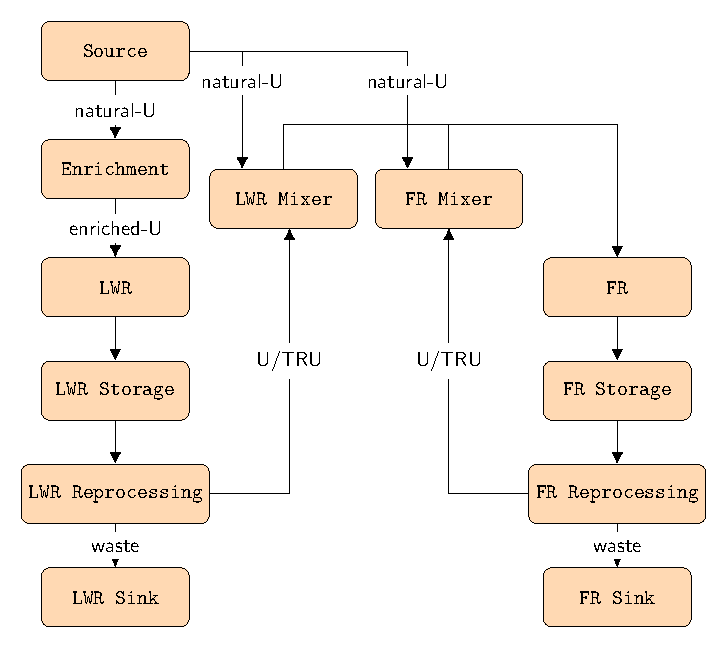
\includegraphics[width=\textwidth]{24-figures/24flow.pdf} 
	\hfill
	\caption{EG01-EG24.}
	\label{fig:24flow}
\end{figure}

\subsection{Flat Power Demand}

This section presents plots of power for all the prediction methods. The power demand is 60000 MW throughout the whole simulation. The input files use the installed capacity feature. Buffer is set to zero, back steps is set to two, and steps takes the default value of one.
Figures \ref{fig:24-NO}, \ref{fig:24-DO}, and \ref{fig:24-SO} display the power supply and demand.
Table \ref{tab:24-power} records the number of steps whit under supply, the cumulative under supply, and the cumulative oversupply.

\begin{figure}[H]
	\centering
	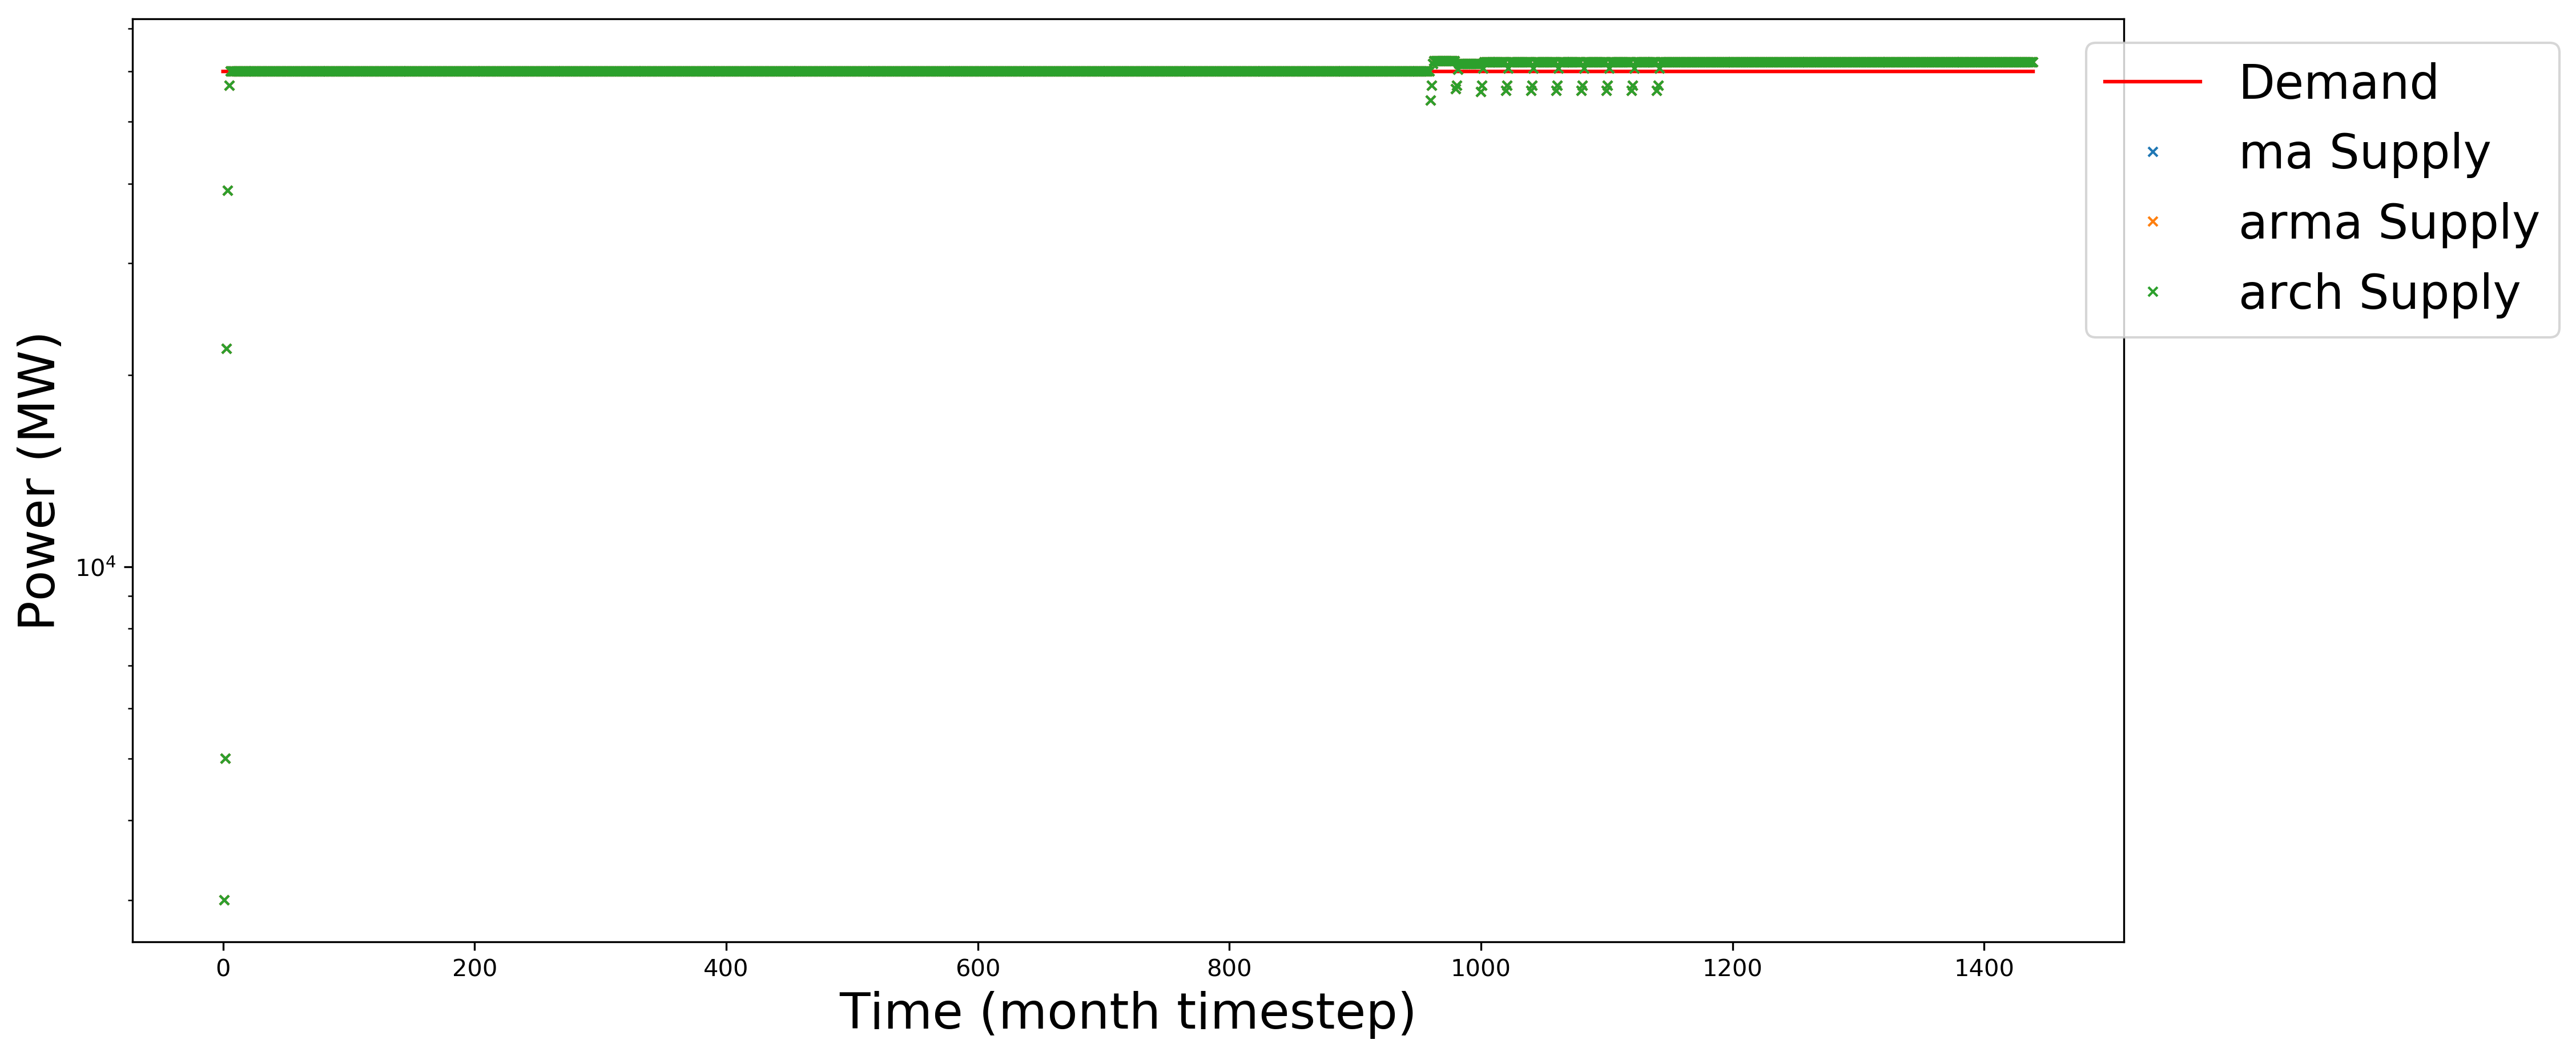
\includegraphics[width=\textwidth]{24-figures/24-power-buffer01.png} 
	\hfill
	\caption{NO algorithms.}
	\label{fig:24-NO}
\end{figure}

\begin{figure}[H]
	\centering
	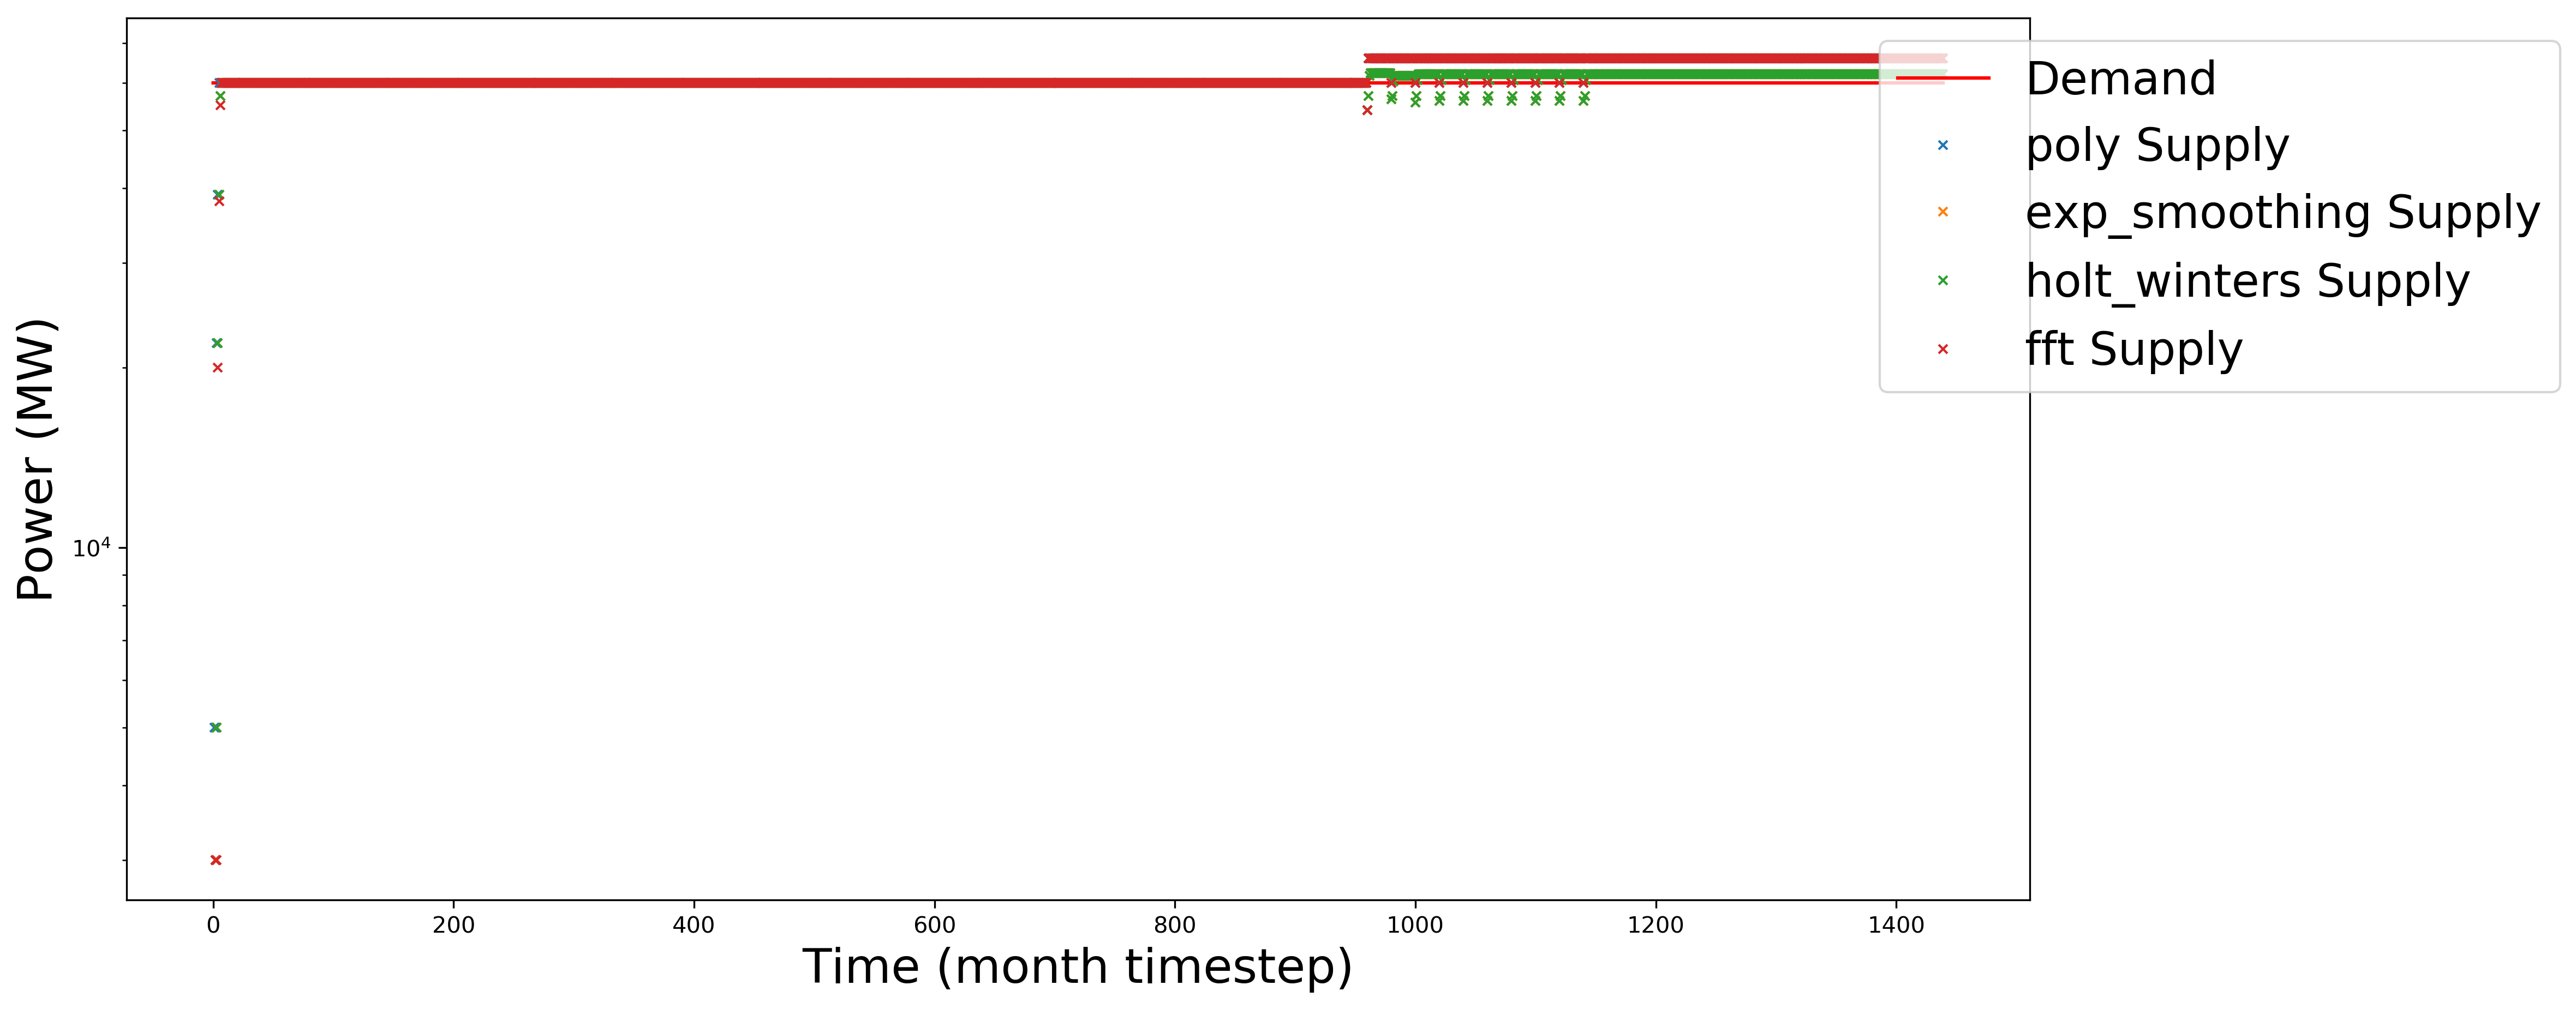
\includegraphics[width=\textwidth]{24-figures/24-power-buffer02.png} 
	\hfill
	\caption{DO algorithms.}
	\label{fig:24-DO}
\end{figure}

\begin{figure}[H]
	\centering
	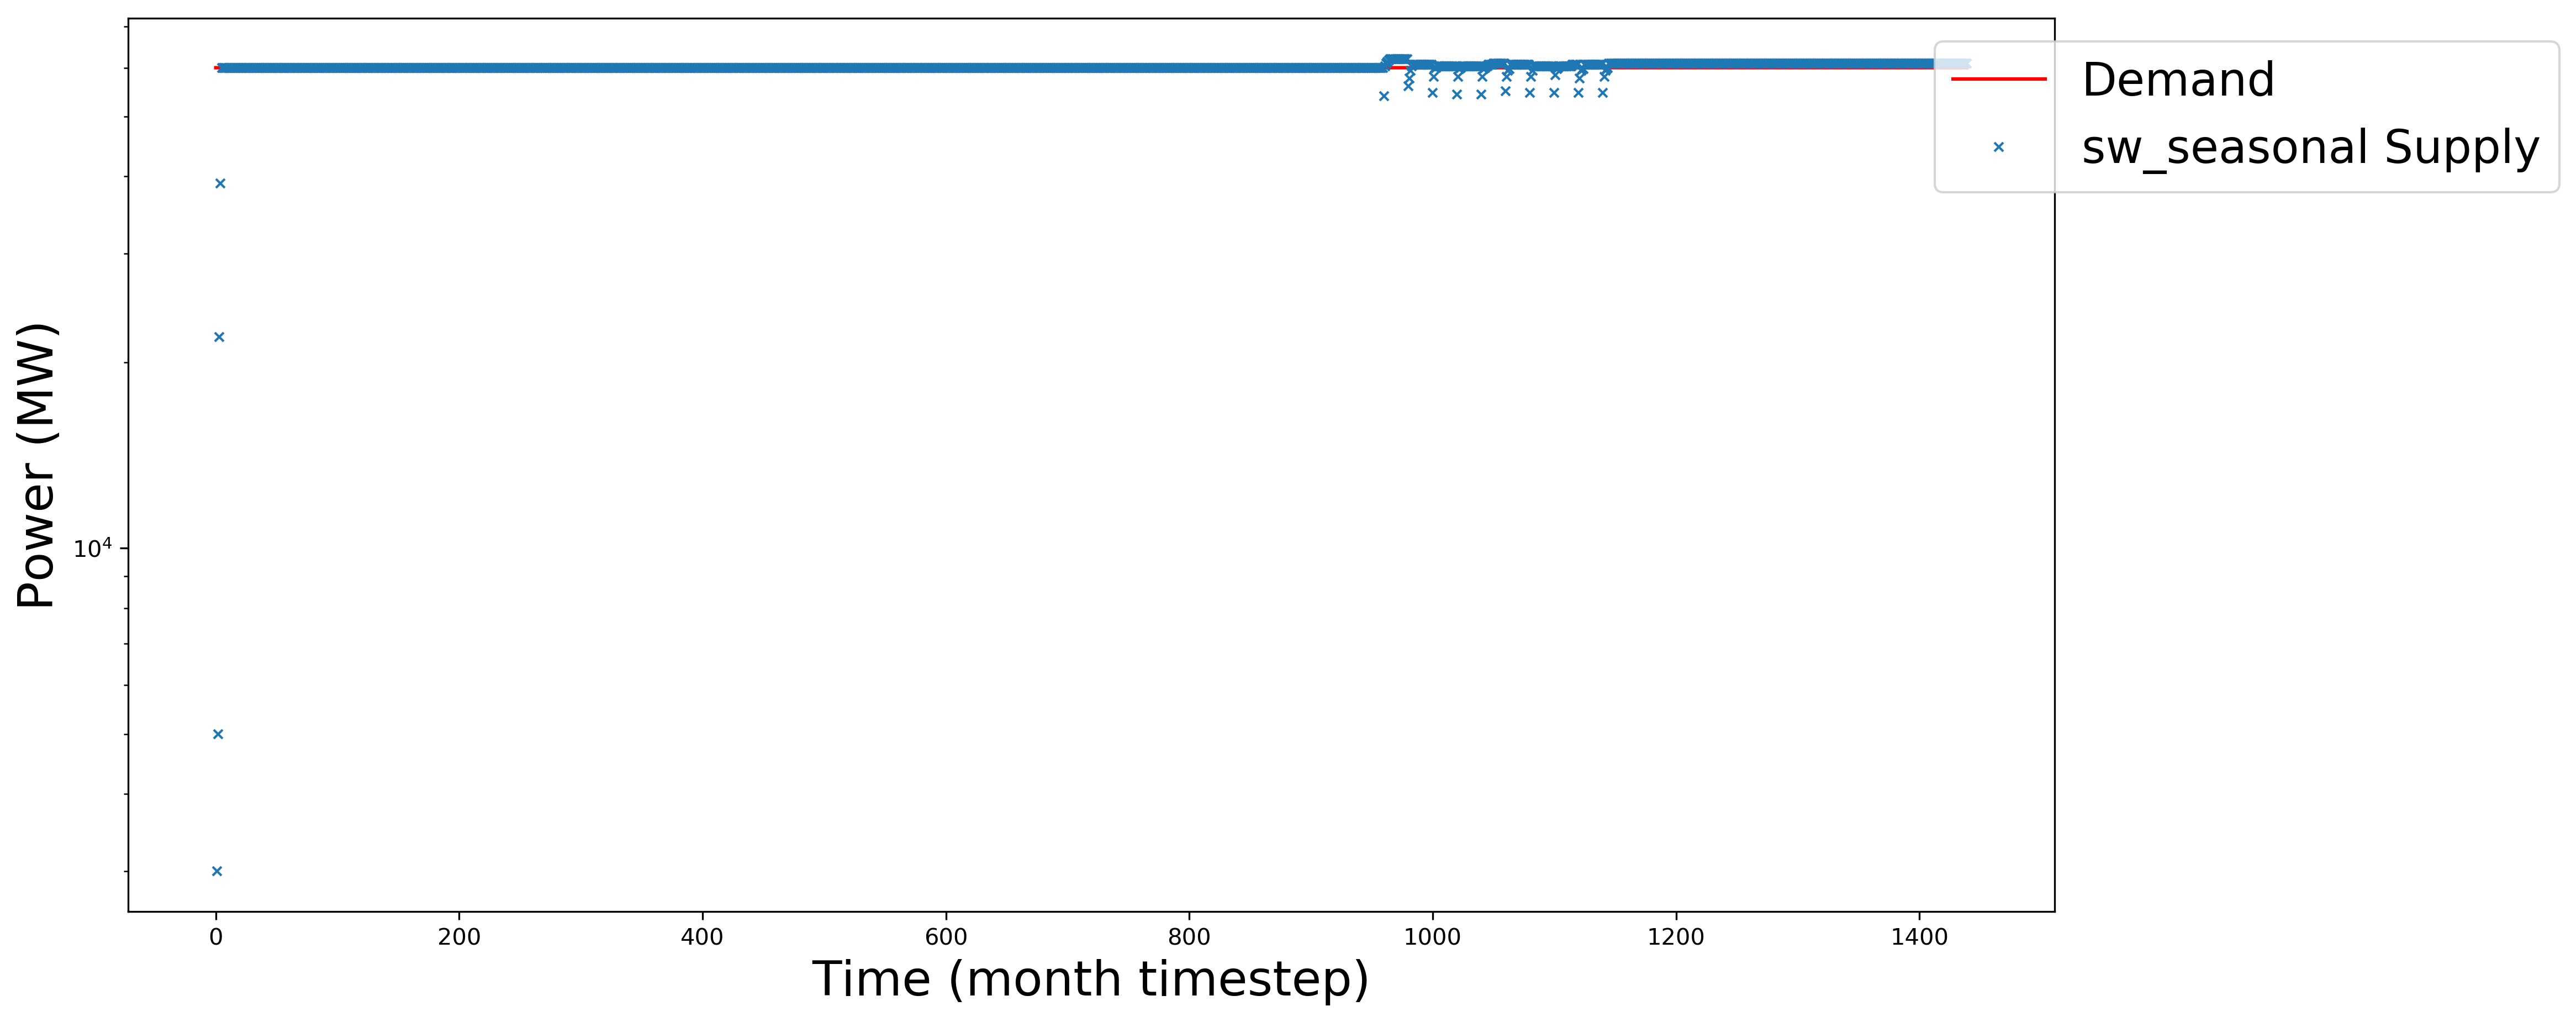
\includegraphics[width=\textwidth]{24-figures/24-power-buffer03.png} 
	\hfill
	\caption{SO algorithms.}
	\label{fig:24-SO}
\end{figure}

\begin{table}[H]
	\centering
	\caption{Undersupply and oversupply of Power for the different algorithms used to calculate EG01-EG24.}
	\label{tab:24-power}
	\begin{tabularx}{\textwidth}{lRRR}
		\hline
		Algorithm & Undersupplied & Cumulative  & Cumulative \\
		& Timesteps     & Undersupply [GW.mo]  & Oversupply [GW.mo] \\ \hline
		MA        & 26 	& 306.0 &  907.8   \\ 
		ARMA      & 26 	& 306.0 &  907.8   \\ 
		ARCH      & 26 	& 306.0 &  907.8   \\ 
		POLY      &  6 	& 235.0 &  2820.5  \\ 
		EXP\_SMOOTHING 	& 27 & 366.0 & 907.8 \\ 
		HOLT-WINTERS  	& 27 & 366.0 & 907.8 \\ 
		FFT       & 8	& 307.0	& 2820.5 \\ 
		SW\_SEASONAL    & 36 & 308.0 & 398.1	\\ \hline
	\end{tabularx}
\end{table}

\subsection{Linearly increasing Power Demand}

This section presents plots of power for all the prediction methods. The power demand increases linearly with the expression $60000 MW + 250*t MW/year$. The input files use the installed capacity feature. Buffer is set to zero, back steps is set to two, and steps takes the default value of one.
Figures \ref{fig:24-lin-NO}, \ref{fig:24-lin-DO}, and \ref{fig:24-lin-SO} display the power supply and demand.
Table \ref{tab:24-lin-power} records the number of steps whit under supply, the cumulative under supply, and the cumulative oversupply.

\begin{figure}[H]
	\centering
	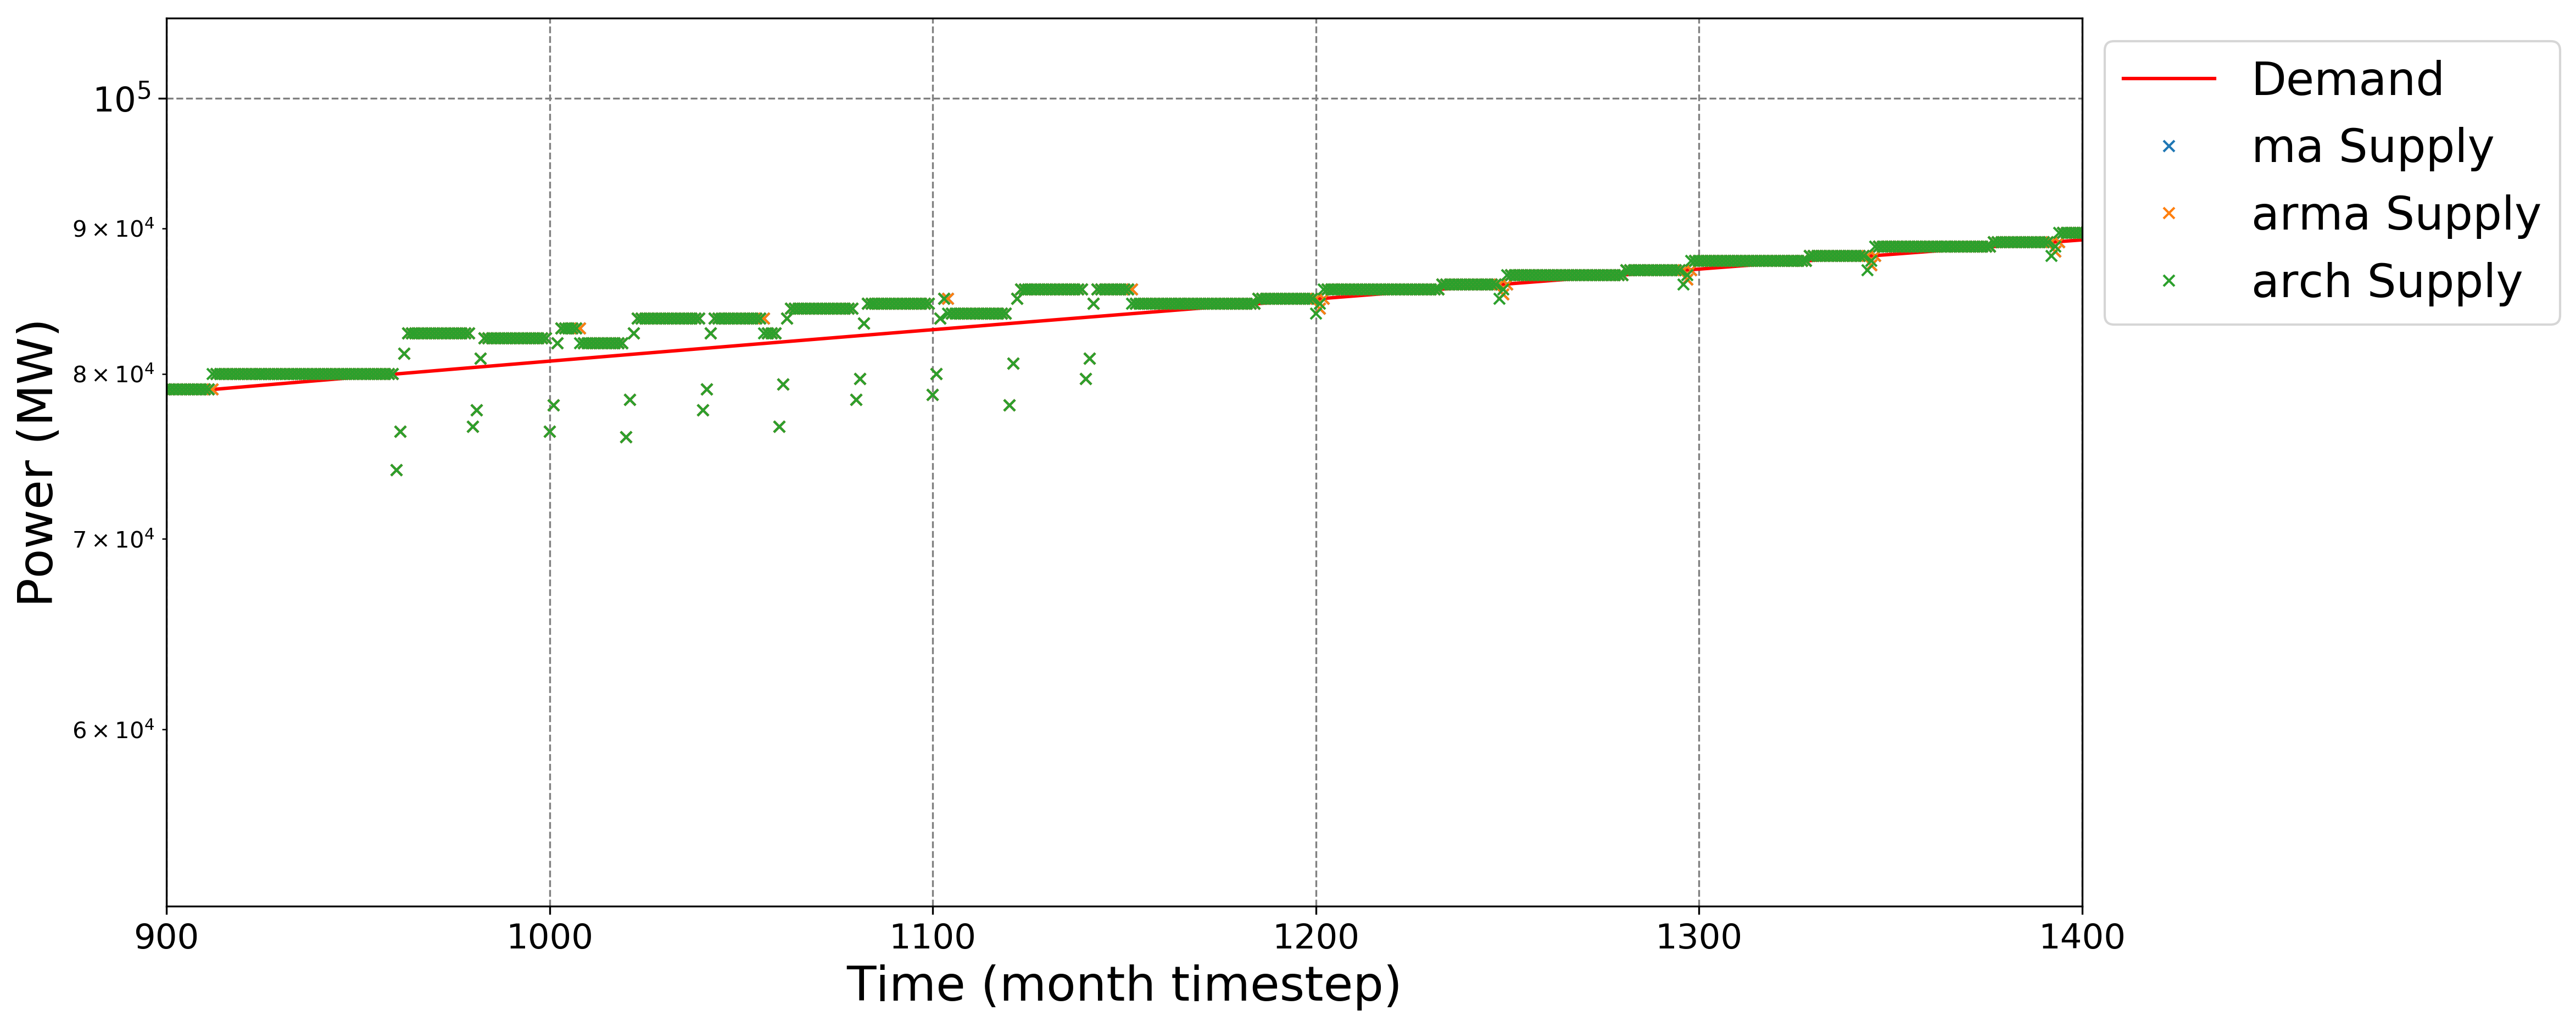
\includegraphics[width=\textwidth]{24-figures/lin-24-power-buffer01.png} 
	\hfill
	\caption{NO algorithms.}
	\label{fig:24-lin-NO}
\end{figure}

\begin{figure}[H]
	\centering
	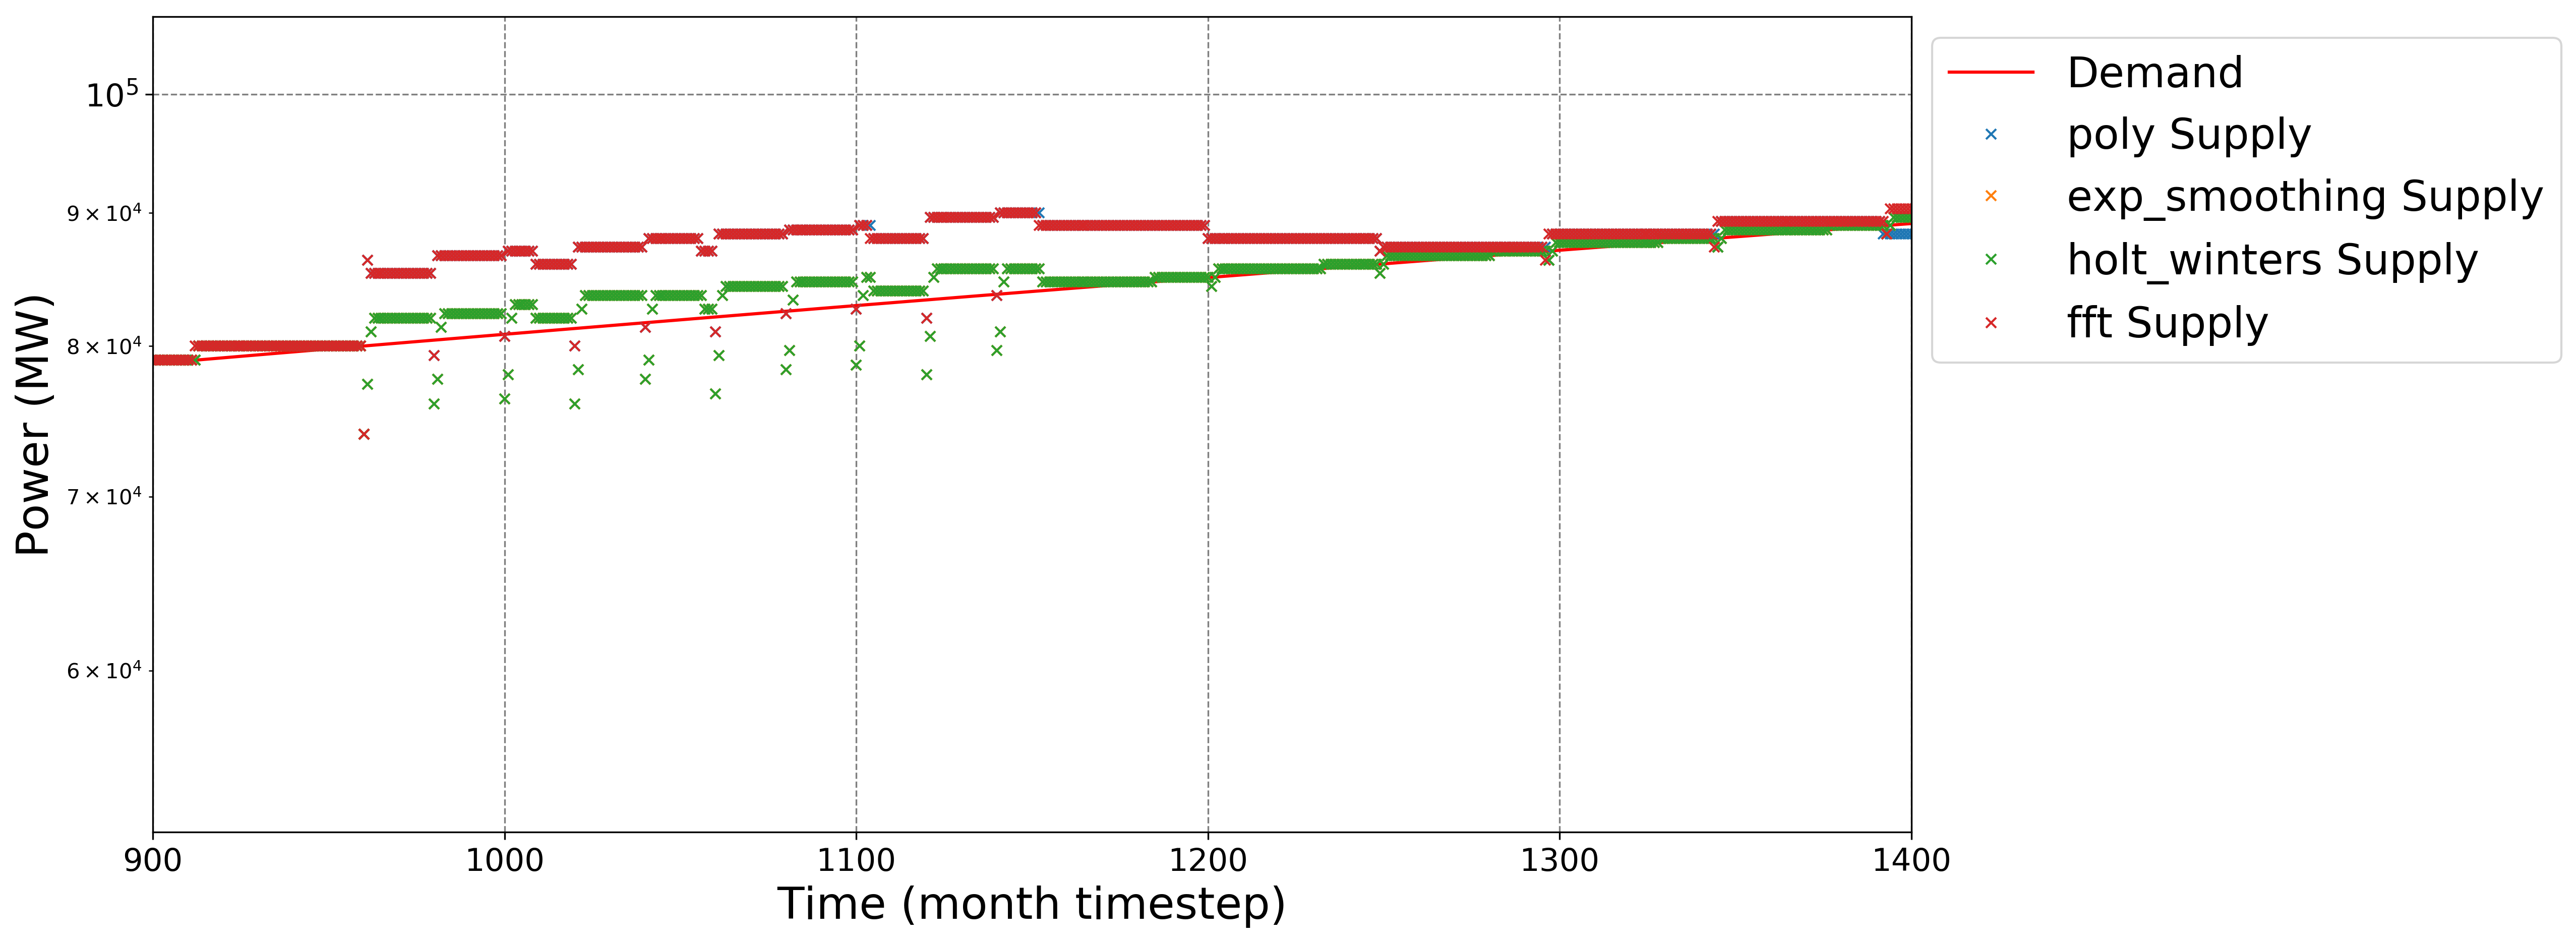
\includegraphics[width=\textwidth]{24-figures/lin-24-power-buffer02.png} 
	\hfill
	\caption{DO algorithms.}
	\label{fig:24-lin-DO}
\end{figure}

\begin{figure}[H]
	\centering
	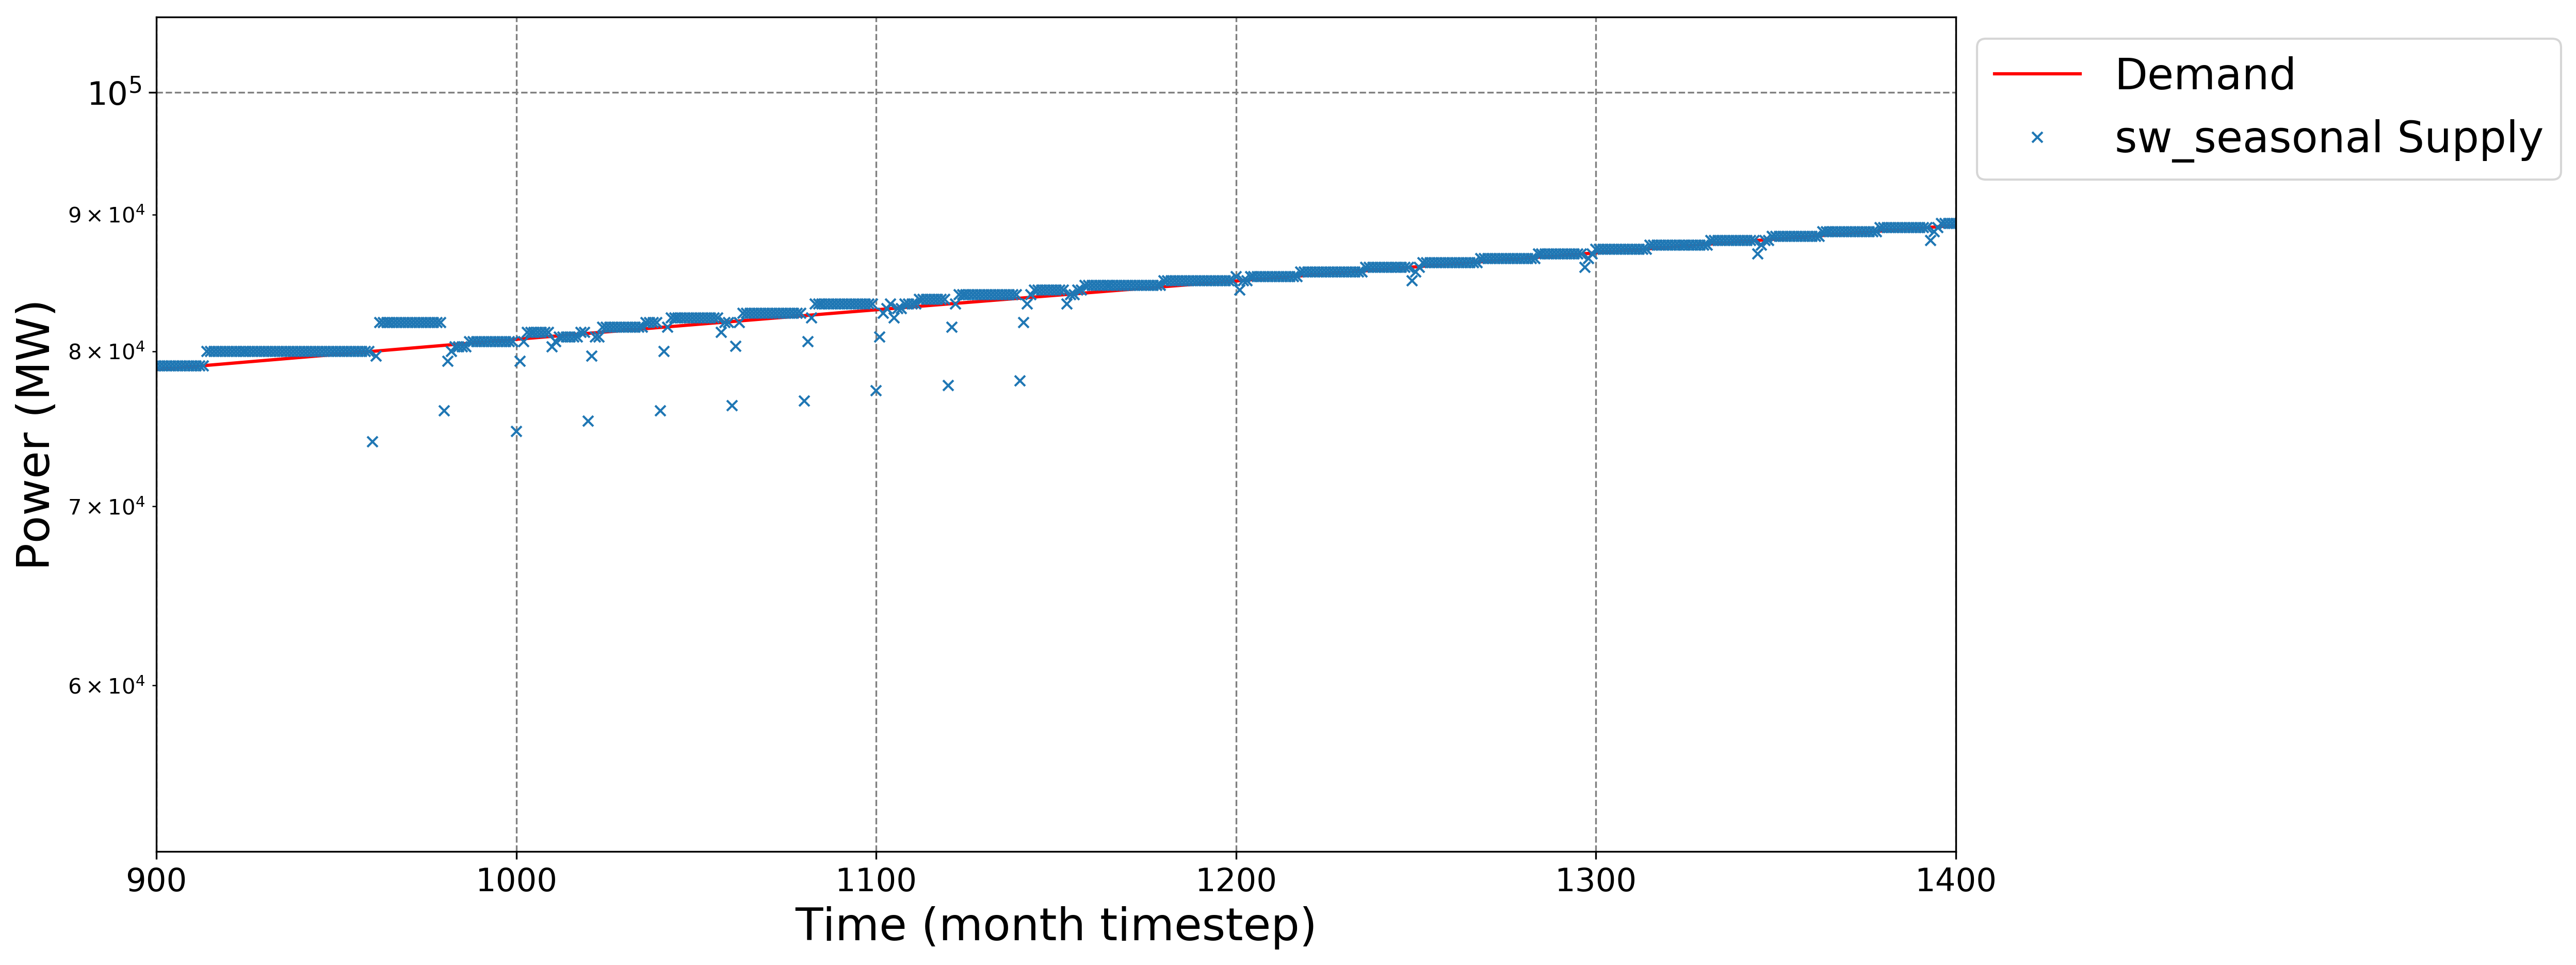
\includegraphics[width=\textwidth]{24-figures/lin-24-power-buffer03.png} 
	\hfill
	\caption{SO algorithms.}
	\label{fig:24-lin-SO}
\end{figure}

\begin{table}[H]
	\centering
	\caption{Undersupply and oversupply of Power for the different algorithms used to calculate EG01-EG24.}
	\label{tab:24-lin-power}
	\begin{tabularx}{\textwidth}{lRRR}
		\hline
		Algorithm & Undersupplied & Cumulative  & Cumulative \\
		& Timesteps     & Undersupply [GW.mo]  & Oversupply [GW.mo] \\ \hline
		MA        & 36 	& 313.7 & 840.9 \\ 
		ARMA      & 36 	& 313.7 & 840.9 \\ 
		ARCH      & 36 	& 316.8 & 859.0 \\ 
		POLY      &  65 & 282.4 & 1974.7 \\ 
		EXP\_SMOOTHING 	& 37 & 373.4 & 828.7 \\ 
		HOLT-WINTERS  	& 37 & 373.4 & 828.7 \\ 
		FFT       & 20	& 315.1	& 2019.1 \\ 
		SW\_SEASONAL    & 107 & 318.8 & 579.09 \\ \hline
	\end{tabularx}
\end{table}

\section{Eg01-Eg29}

Figure \ref{fig:29flow} shows the flow of Eg01-Eg29.

\begin{figure}[H]
	\centering
	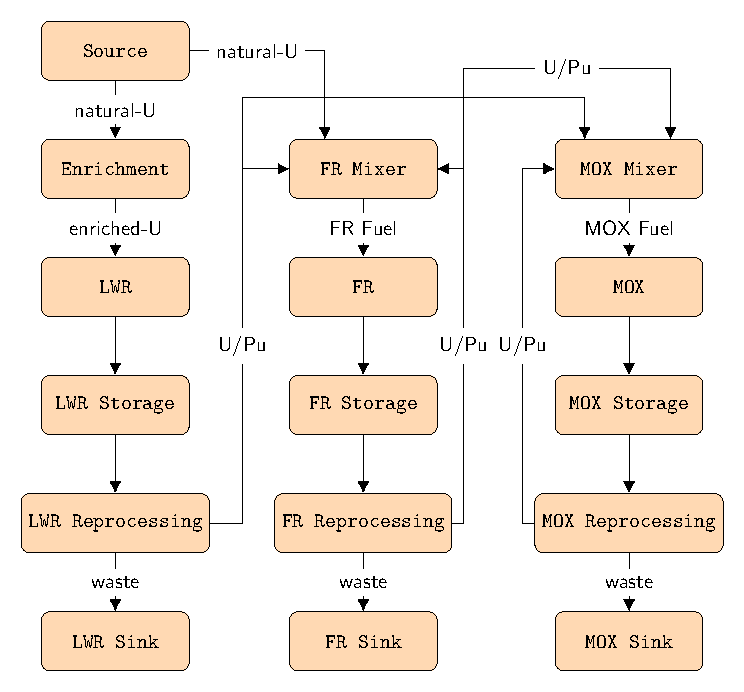
\includegraphics[width=\textwidth]{29-figures/29flow.pdf} 
	\hfill
	\caption{EG01-EG29.}
	\label{fig:29flow}
\end{figure}

\subsection{Power}

This section presents plots of power for all the prediction methods. The power demand is 60000 MW throughout the whole simulation. The input files use the installed capacity feature. Buffer is set to zero, back steps is set to two, and steps takes the default value of one.
Figures \ref{fig:29-NO}, \ref{fig:29-DO}, and \ref{fig:29-SO} display the power supply and demand.
Table \ref{tab:29-power} records the number of steps with under supply, the cumulative under supply, and the cumulative oversupply.

\begin{figure}[H]
	\centering
	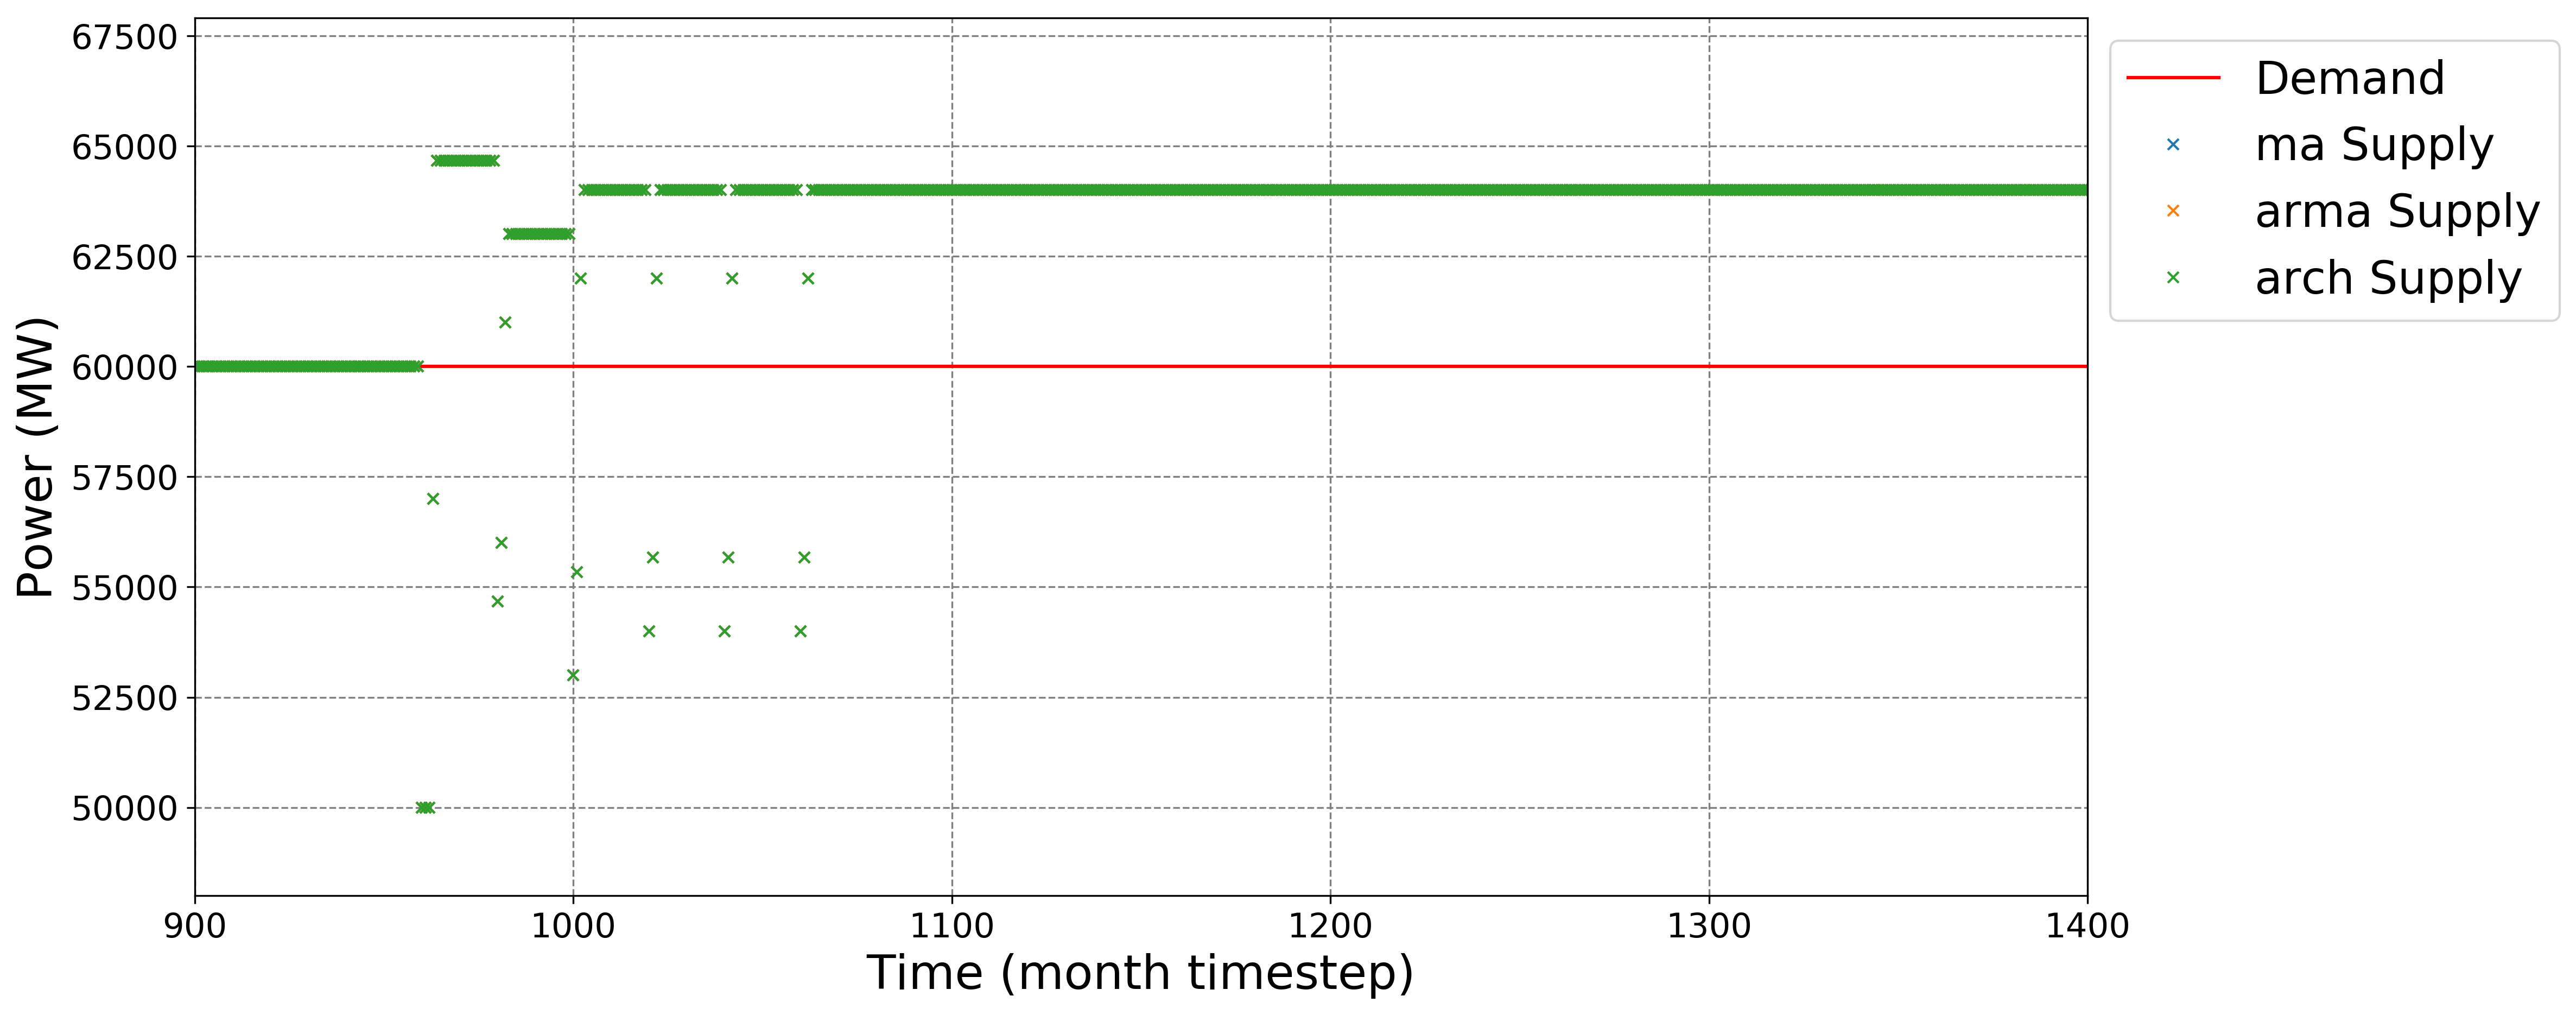
\includegraphics[width=\textwidth]{29-figures/29-power0-buffer01.png} 
	\hfill
	\caption{NO algorithms.}
	\label{fig:29-NO}
\end{figure}

\begin{figure}[H]
	\centering
	\includegraphics[width=\textwidth]{29-figures/29-power0-buffer02.png} 
	\hfill
	\caption{DO algorithms.}
	\label{fig:29-DO}
\end{figure}

\begin{figure}[H]
	\centering
	\includegraphics[width=\textwidth]{29-figures/29-power0-buffer03.png} 
	\hfill
	\caption{SO algorithms.}
	\label{fig:29-SO}
\end{figure}

\begin{table}[H]
	\centering
	\caption{Undersupply and oversupply of Power for the different algorithms used to calculate EG01-EG29.}
	\label{tab:29-power}
	\begin{tabularx}{\textwidth}{lRRR}
		\hline
		Algorithm & Undersupplied & Cumulative  & Cumulative \\
		& Timesteps     & Undersupply [GW.mo]  & Oversupply [GW.mo] \\ \hline
		MA        & 15 	& 145.0 & 1847.0 \\ 
		ARMA      & 15 	& 145.0 & 1847.0 \\ 
		ARCH      & 15 	& 145.0 & 1846.9 \\ 
		POLY      &  4 	& 90.0 & 4720.3 \\ 
		EXP\_SMOOTHING 	& 16 & 205.0 & 1847.0 \\ 
		HOLT-WINTERS  	& 16 & 205.0 & 1847.0 \\ 
		FFT       &  5	& 150.0	& 4898.0 \\ 
		SW\_SEASONAL    & 14 & 139.0 & 798.9 \\ \hline
	\end{tabularx}
\end{table}

\subsection{Buffer}

This section presents a sensitivity analysis for different values of the buffer. Figure \ref{fig:29-buff} shows a comparison of the cumulative under supply for different buffer sizes.

Figures \ref{fig:29-buf-ma} to \ref{fig:29-buf-fft} display a comparison for some of the methods of the power supply for different buffer sizes.

The input files use the installed capacity feature. Buffer takes the values 0, 2000, 4000, 6000, and 8000. Back steps is set to two, and steps takes the default value of one.

\begin{figure}[H]
	\centering
	\includegraphics[width=\textwidth]{29-figures/29-sens-buffer.png} 
	\hfill
	\caption{Sensitivity analysis for different buffer sizes for some prediction algorithms.}
	\label{fig:29-buff}
\end{figure}

\begin{figure}[H]
	\centering
	\includegraphics[width=\textwidth]{29-figures/29-power-buffer-ma.png} 
	\hfill
	\caption{Power supply for different buffer sizes using ma.}
	\label{fig:29-buf-ma}
\end{figure}

\begin{figure}[H]
	\centering
	\includegraphics[width=\textwidth]{29-figures/29-power-buffer-arma.png} 
	\hfill
	\caption{Power supply for different buffer sizes using arma.}
	\label{fig:29-buf-arma}
\end{figure}

\begin{figure}[H]
	\centering
	\includegraphics[width=\textwidth]{29-figures/29-power-buffer-arch.png} 
	\hfill
	\caption{Power supply for different buffer sizes using arch.}
	\label{fig:29-buf-arch}
\end{figure}

\begin{figure}[H]
	\centering
	\includegraphics[width=\textwidth]{29-figures/29-power-buffer-poly.png} 
	\hfill
	\caption{Power supply for different buffer sizes using poly.}
	\label{fig:29-buf-poly}
\end{figure}

\begin{figure}[H]
	\centering
	\includegraphics[width=\textwidth]{29-figures/29-power-buffer-exp_smoothing.png} 
	\hfill
	\caption{Power supply for different buffer sizes using exp\_smoothing.}
	\label{fig:29-buf-exp_smoothing}
\end{figure}

\begin{figure}[H]
	\centering
	\includegraphics[width=\textwidth]{29-figures/29-power-buffer-holt_winters.png} 
	\hfill
	\caption{Power supply for different buffer sizes using holt\_winters.}
	\label{fig:29-buf-hots_winters}
\end{figure}

\begin{figure}[H]
	\centering
	\includegraphics[width=\textwidth]{29-figures/29-power-buffer-fft.png} 
	\hfill
	\caption{Power supply for different buffer sizes using fft.}
	\label{fig:29-buf-fft}
\end{figure}

\subsection{Steps forward}

This section presents a sensitivity analysis for different values of steps.
Figure \ref{fig:29-steps} shows a comparison of the cumulative under supply for different values of steps forward.

Figures \ref{fig:29-ste-ma} to \ref{fig:29-ste-fft} display a comparison for some of the methods of the power supply for different steps.

The input files use the installed capacity feature. Buffer is set to zero, back steps is set to two, and steps takes the values 1, 2, 3, 4, and 5.

\begin{figure}[H]
	\centering
	\includegraphics[width=\textwidth]{29-figures/29-sens-steps.png} 
	\hfill
	\caption{Sensitivity analysis for different number of steps forward for some prediction algorithms.}
	\label{fig:29-steps}
\end{figure}

\begin{figure}[H]
	\centering
	\includegraphics[width=\textwidth]{29-figures/29-power-buffer0-ma-steps.png} 
	\hfill
	\caption{Power supply for different values of steps forward using ma.}
	\label{fig:29-ste-ma}
\end{figure}

\begin{figure}[H]
	\centering
	\includegraphics[width=\textwidth]{29-figures/29-power-buffer0-arma-steps.png} 
	\hfill
	\caption{Power supply for different values of steps forward using arma.}
	\label{fig:29-ste-arma}
\end{figure}

\begin{figure}[H]
	\centering
	\includegraphics[width=\textwidth]{29-figures/29-power-buffer0-arch-steps.png} 
	\hfill
	\caption{Power supply for different values of steps forward using arch.}
	\label{fig:29-ste-arch}
\end{figure}

\begin{figure}[H]
	\centering
	\includegraphics[width=\textwidth]{29-figures/29-power-buffer0-poly-steps.png} 
	\hfill
	\caption{Power supply for different values of steps forward using poly.}
	\label{fig:29-ste-poly}
\end{figure}

\begin{figure}[H]
	\centering
	\includegraphics[width=\textwidth]{29-figures/29-power-buffer0-exp_smoothing-steps.png} 
	\hfill
	\caption{Power supply for different values of steps forward using exp\_smoothing.}
	\label{fig:29-ste-exp_smoothing}
\end{figure}

\begin{figure}[H]
	\centering
	\includegraphics[width=\textwidth]{29-figures/29-power-buffer0-holt_winters-steps.png} 
	\hfill
	\caption{Power supply for different values of steps forward using holt\_winters.}
	\label{fig:29-ste-hots_winters}
\end{figure}

\begin{figure}[H]
	\centering
	\includegraphics[width=\textwidth]{29-figures/29-power-buffer0-fft-steps.png} 
	\hfill
	\caption{Power supply for different values of steps forward using fft.}
	\label{fig:29-ste-fft}
\end{figure}

\subsection{Different commodities}

Table \ref{tab:29-commodities} shows the name of the variables used in the simulations and what they represent in the cycle. Table \ref{tab:29-commod} presents the number of steps of under supply, cumulative under supply, and cumulative oversupply for some of the commodities.

In this simulation, front-end commodities are power, sourceout, enrichmentout, frmixerout, and moxmixerout. All the rest of the commodities are back-end.

\begin{table}[H]
	\centering
	\caption{Commodity names used in the simulation of EG01-EG29.}
	\label{tab:29-commodities}
	\begin{tabularx}{\textwidth}{lLL}
		\hline
		Commodity name  & Figures & Represents \\ \hline
		power           & \ref{fig:29-power} & Power \\
		sourceout       & \ref{fig:29-sourceout} & Natural-U \\
		enrichmentout   & \ref{fig:29-enrichmentout} & Enriched-U \\
		frmixerout      &  \ref{fig:29-frmixerout} & FR fuel \\
    	moxmixerout     &  \ref{fig:29-moxmixerout} & MOX fuel \\
		lwrout          & \ref{fig:29-out1} & Spent fuel of LWRs \\
		frout           & \ref{fig:29-frout} & Spent fuel of FRs \\
		frout           & \ref{fig:29-moxout} & Spent fuel of MOX LWRs \\
		lwrstorageout   & \ref{fig:29-storageout1} & Cooled down spent fuel of LWRs \\
		frstorageout    & \ref{fig:29-frstorageout} & Cooled down spent fuel of FRs \\	
		moxstorageout    & \ref{fig:29-moxstorageout} & Cooled down spent fuel of MOX LWRs \\	
		lwrpu   & \ref{fig:29-pu1} & Pu from spent fuel of LWRs \\
		frpu    & \ref{fig:29-frpu} & Pu from spent fuel of FRs \\
		moxpu    & \ref{fig:29-moxpu} & Pu from spent fuel of MOX LWRs \\
		lwrreprocessingwaste & \ref{fig:29-lwrreprocessingwaste} & Waste from the reprocessing of spent fuel of LWRs \\
		frreprocessingwaste & \ref{fig:29-frreprocessingwaste} & Waste from the reprocessing of spent fuel of FRs \\
		moxreprocessingwaste & \ref{fig:29-moxreprocessingwaste} & Waste from the reprocessing of spent fuel of MOX LWRs \\ \hline
			
	\end{tabularx}
\end{table}

\begin{figure}[H]
	\centering
	\includegraphics[width=\textwidth]{29-figures/0-poly-power.png} 
	\hfill
	\caption{Supply and demand of the commodity power.}
	\label{fig:29-power}
\end{figure}

\begin{figure}[H]
	\centering
	\begin{subfigure}[]{0.45\textwidth}
		\centering
		\includegraphics[width=\linewidth]{29-figures/0-poly-sourceout.png} 
		\caption{Commodity sourceout.}
		\label{fig:29-sourceout}
	\end{subfigure}
	\vspace{1cm}
	\begin{subfigure}[]{0.45\textwidth}
		\centering
		\includegraphics[width=\linewidth]{29-figures/0-poly-enrichmentout.png} 
		\caption{Commodity enrichmentout.}
		\label{fig:29-enrichmentout}
	\end{subfigure}
	\hfill
	\caption{Supply and demand of different commodities for the prediction method poly.}
	\label{fig:29-front}
\end{figure}

\begin{figure}[H]
	\centering
	\begin{subfigure}[]{0.45\textwidth}
		\centering
		\includegraphics[width=\linewidth]{29-figures/0-poly-frmixerout.png} 
		\caption{Commodity frmixerout.}
		\label{fig:29-frmixerout}
	\end{subfigure}
	\vspace{1cm}
	\begin{subfigure}[]{0.45\textwidth}
		\centering
		\includegraphics[width=\linewidth]{29-figures/0-poly-moxmixerout.png} 
		\caption{Commodity moxmixerout.}
		\label{fig:29-moxmixerout}
	\end{subfigure}
	\hfill
	\caption{Supply and demand of different commodities for the prediction method poly.}
	\label{fig:29-mix}
\end{figure}

\begin{figure}[H]
	\centering
	\includegraphics[width=\textwidth]{29-figures/0-poly-lwrout.png} 
	\hfill
	\caption{Supply and demand of the commodity lwrout.}
	\label{fig:29-out1}
\end{figure}

\begin{figure}[H]
	\centering
	\begin{subfigure}[]{0.45\textwidth}
		\centering
		\includegraphics[width=\linewidth]{29-figures/0-poly-frout.png} 
		\caption{Commodity frout.}
		\label{fig:29-frout}
	\end{subfigure}
	\vspace{1cm}
	\begin{subfigure}[]{0.45\textwidth}
		\centering
		\includegraphics[width=\linewidth]{29-figures/0-poly-moxout.png} 
		\caption{Commodity moxout.}
		\label{fig:29-moxout}
	\end{subfigure}
	\hfill
	\caption{Supply and demand of different commodities for the prediction method poly.}
	\label{fig:29-out2}
\end{figure}

\begin{figure}[H]
	\centering
	\includegraphics[width=\textwidth]{29-figures/0-poly-lwrstorageout.png} 
	\hfill
	\caption{Supply and demand of the commodity lwrstorageout.}
	\label{fig:29-storageout1}
\end{figure}

\begin{figure}[H]
	\centering
	\begin{subfigure}[t]{0.45\textwidth}
		\centering
		\includegraphics[width=\linewidth]{29-figures/0-poly-frstorageout.png} 
		\caption{Commodity frstorageout.}
		\label{fig:29-frstorageout}
	\end{subfigure}
	\vspace{1cm}
	\begin{subfigure}[t]{0.45\textwidth}
		\centering
		\includegraphics[width=\linewidth]{29-figures/0-poly-moxstorageout.png} 
		\caption{Commodity moxstorageout.}
		\label{fig:29-moxstorageout}
	\end{subfigure}
	\hfill
	\caption{Supply and demand of different commodities for the prediction method poly.}
	\label{fig:29-storageout2}
\end{figure}

\begin{figure}[H]
	\centering
	\includegraphics[width=\textwidth]{29-figures/0-poly-lwrpu.png} 
	\hfill
	\caption{Supply and demand of the commodity lwrpu.}
	\label{fig:29-pu1}
\end{figure}

\begin{figure}[H]
	\centering
	\begin{subfigure}[t]{0.45\textwidth}
		\centering
		\includegraphics[width=\linewidth]{23-figures/0-poly-frpu.png} 
		\caption{Commodity frpu.}
		\label{fig:29-frpu}
	\end{subfigure}
	\vspace{1cm}
	\begin{subfigure}[t]{0.45\textwidth}
		\centering
		\includegraphics[width=\linewidth]{29-figures/0-poly-moxpu.png} 
		\caption{Commodity moxpu.}
		\label{fig:29-moxpu}
	\end{subfigure}
	\hfill
	\caption{Supply and demand of different commodities for the prediction method poly.}
	\label{fig:29-pu2}
\end{figure}

\begin{figure}[H]
	\centering
	\includegraphics[width=\textwidth]{29-figures/0-poly-lwrreprocessingwaste.png} 
	\hfill
	\caption{Supply and demand of the commodity lwrreprocessingwaste.}
	\label{fig:29-lwrreprocessingwaste}
\end{figure}

\begin{figure}[H]
	\centering
	\begin{subfigure}[t]{0.45\textwidth}
		\centering
		\includegraphics[width=\linewidth]{23-figures/0-poly-frreprocessingwaste.png} 
		\caption{Commodity frreprocessingwaste.}
		\label{fig:29-frreprocessingwaste}
	\end{subfigure}
	\vspace{1cm}
	\begin{subfigure}[t]{0.45\textwidth}
		\centering
		\includegraphics[width=\linewidth]{29-figures/0-poly-moxreprocessingwaste.png} 
		\caption{Commodity moxreprocessingwaste.}
		\label{fig:29-moxreprocessingwaste}
	\end{subfigure}
	\hfill
	\caption{Supply and demand of different commodities for the prediction method poly.}
	\label{fig:29-waste}
\end{figure}

\begin{table}[H]
	\centering
	\caption{Undersupply and oversupply of different commodities using poly to calculate EG01-EG29.}
	\label{tab:29-commod}
	\begin{tabularx}{\textwidth}{lRRR}
		\hline
		Commodity & Undersupplied & Cumulative  & Cumulative \\
		& Timesteps & Undersupply [$10^3$Kg]  & Oversupply [$10^6$Kg] \\ \hline
		sourceout & 1 & 34394.0  & 132319869.5 \\ 
		enrichmentout & 1 & 16126.1 & 102751545581.6 \\

		lwrout & 1 & 1791.8 & - \\
		frout & 1 & 142.2 & - \\
		moxout & 1 & 265.0 & - \\

		frmixerout & 2 & 284.4 & 124827.3 \\
        moxmixerout & 2 & 530.1 & 354541.5 \\

		lwrstorageout & 1 & 1791.8 & - \\
		frstorageout & 1 & 142.2 & - \\
		moxstorageout & 1 & 265.0 & - \\ \hline
	\end{tabularx}
\end{table}

\section{Eg01-Eg30}

Figure \ref{fig:30flow} shows the flow of Eg01-Eg30.

\begin{figure}[H]
	\centering
	\includegraphics[width=\textwidth]{30-figures/30flow.pdf} 
	\hfill
	\caption{EG01-EG30.}
	\label{fig:30flow}
\end{figure}

\subsection{Flat Power Demand}

This section presents plots of power for all the prediction methods. The power demand is 60000 MW throughout the whole simulation. The input files use the installed capacity feature. Buffer is set to zero, back steps is set to two, and steps takes the default value of one.
Figures \ref{fig:30-NO}, \ref{fig:30-DO}, and \ref{fig:30-SO} display the power supply and demand.
Table \ref{tab:30-power} records the number of steps whit under supply, the cumulative under supply, and the cumulative oversupply.

\begin{figure}[H]
	\centering
	\includegraphics[width=\textwidth]{30-figures/30-power-buffer01.png} 
	\hfill
	\caption{NO algorithms.}
	\label{fig:30-NO}
\end{figure}

\begin{figure}[H]
	\centering
	\includegraphics[width=\textwidth]{30-figures/30-power-buffer02.png} 
	\hfill
	\caption{DO algorithms.}
	\label{fig:30-DO}
\end{figure}

\begin{figure}[H]
	\centering
	\includegraphics[width=\textwidth]{30-figures/30-power-buffer03.png} 
	\hfill
	\caption{SO algorithms.}
	\label{fig:30-SO}
\end{figure}

\begin{table}[H]
	\centering
	\caption{Undersupply and oversupply of Power for the different algorithms used to calculate EG01-EG24.}
	\label{tab:30-power}
	\begin{tabularx}{\textwidth}{lRRR}
		\hline
		Algorithm & Undersupplied & Cumulative  & Cumulative \\
		& Timesteps     & Undersupply [GW.mo]  & Oversupply [GW.mo] \\ \hline
		MA        & 15 & 144.0 & 1718.7 \\ 
		ARMA      & 15 & 144.0 & 1718.7 \\ 
		ARCH      & 15 & 144.0 & 1718.7 \\ 
		POLY      & 4  & 90.0 & 5026.5 \\ 
		EXP\_SMOOTHING 	& 16 & 204.0 & 1718.7 \\ 
		HOLT-WINTERS  	& 16 & 204.0 & 1718.7 \\ 
		FFT       & 5 & 150.0 & 5044.5 \\ 
		SW\_SEASONAL    & 14 & 141.0 & 784.0 \\ \hline
	\end{tabularx}
\end{table}

\subsection{Linearly increasing Power Demand}

This section presents plots of power for all the prediction methods. The power demand increases linearly with the expression $60000 MW + 250*t MW/year$. The input files use the installed capacity feature. Buffer is set to zero, back steps is set to two, and steps takes the default value of one.
Figures \ref{fig:30-lin-NO}, \ref{fig:30-lin-DO}, and \ref{fig:30-lin-SO} display the power supply and demand.
Table \ref{tab:30-lin-power} records the number of steps whit under supply, the cumulative under supply, and the cumulative oversupply.

\begin{figure}[H]
	\centering
	\includegraphics[width=\textwidth]{30-figures/lin-30-power-buffer01.png} 
	\hfill
	\caption{NO algorithms.}
	\label{fig:30-lin-NO}
\end{figure}

\begin{figure}[H]
	\centering
	\includegraphics[width=\textwidth]{30-figures/lin-30-power-buffer02.png} 
	\hfill
	\caption{DO algorithms.}
	\label{fig:30-lin-DO}
\end{figure}

\begin{figure}[H]
	\centering
	\includegraphics[width=\textwidth]{30-figures/lin-30-power-buffer03.png} 
	\hfill
	\caption{SO algorithms.}
	\label{fig:30-lin-SO}
\end{figure}

\begin{table}[H]
	\centering
	\caption{Undersupply and oversupply of Power for the different algorithms used to calculate EG01-EG24.}
	\label{tab:30-lin-power}
	\begin{tabularx}{\textwidth}{lRRR}
		\hline
		Algorithm & Undersupplied & Cumulative  & Cumulative \\
		& Timesteps     & Undersupply [GW.mo]  & Oversupply [GW.mo] \\ \hline
		MA        & 24 & 152.3 & 1334.1 \\ 
		ARMA      & 24 & 152.3 & 1334.1 \\ 
		ARCH      & 21 & 152.1 & 1355.9 \\ 
		POLY      &  9 & 92.5 & 3073.1 \\ 
		EXP\_SMOOTHING 	& 25 & 211.6 & 1317.8 \\ 
		HOLT-WINTERS  	& 25 & 211.6 & 1317.8 \\ 
		FFT       & 9 & 152.5 & 3079.4 \\ 
		SW\_SEASONAL  & 51 & 147.3 & 873.4 \\ \hline
	\end{tabularx}
\end{table}

\end{document}